\documentclass[11pt]{article}\usepackage[margin=1in]{geometry}\usepackage{amsmath,amssymb,amsthm,mathtools}\usepackage{graphicx}\graphicspath{{figures/}{../figures/}{figs/}{./}}\usepackage{enumitem}\usepackage{hyperref}\usepackage{cleveref}\usepackage{tikz}\usetikzlibrary{arrows.meta,positioning,calc,shapes.geometric}\usepackage{float}\usepackage{rotating}\usepackage[most]{tcolorbox}\usepackage{kotex}\usepackage{booktabs}\usepackage{longtable}\emergencystretch=1.6em\tolerance=2000 \crefname{assumption}{Assumption}{Assumptions}\Crefname{assumption}{Assumption}{Assumptions}\crefname{definition}{Definition}{Definitions}\Crefname{definition}{Definition}{Definitions}\crefname{proposition}{Proposition}{Propositions}\Crefname{proposition}{Proposition}{Propositions}\crefname{fact}{Fact}{Facts}\Crefname{fact}{Fact}{Facts} \newtheorem{assumption}{Assumption}\newtheorem{definition}{Definition}\newtheorem{lemma}{Lemma}\newtheorem{proposition}{Proposition}\newtheorem{theorem}{Theorem}\newtheorem{corollary}{Corollary}\newtheorem{fact}{Fact}\theoremstyle{remark}\newtheorem{remark}{Remark} \newcommand{\R}{\mathbb{R}}\newcommand{\xb}{\bar x}\newcommand{\Ab}{\bar A}\newcommand{\By}{\bar B_y}\newcommand{\U}{\mathcal U}\newcommand{\Z}{\mathcal Z}
\newcommand{\Cset}{\mathcal C}\newcommand{\Pcl}{\mathcal P}\newcommand{\Kset}{\mathcal K}

\title{적응 제어 철학을 가진 RL policy의 사양 (v3):\\ 에너지 장부로 결합된 학습}
\author{Junhyeok Yoon}
\date{2026년 11월 17일 (개정 17)}

\begin{document}
\maketitle

\begin{abstract}
이 문서는 적응 제어의 철학을 구조에 담은 RL policy의 세 번째 설계(v3)를 정의한다. 앞선 설계(v2)의 실패에서 배운 다섯 가지 교훈 위에서, v3는 actuator 수준의 손(가상 impedance와, 정지 상태에서 측정된 mismatch로 갱신되는 적응 기억), 관절 한계 근처에서만 개입하는 제약층, 실제 actuator 일률을 지불하는 energy tank와 접촉 guard, 그리고 뇌(task policy)로 이루어진다. Plant class에는 관절 torque sensing이 포함된다. Tank는 손의 구조와 무관하게 접촉 port의 passivity를 주고, 남은 예산, 능력 사용, 손이 배운 부하로 이루어진 장부가 손에서 뇌로 가는 정보가 된다. 모든 층은 같은 rollout에서 함께 학습되고 각 층은 자기 역할에 귀속되는 신호를 받으며, 역할이 의도대로 학습되었는지는 별도의 검증 protocol로 확인한다. 이 문서는 대상, 구조, 학습 framework, 요구 사항, 구현·학습·검증 계획을 정하고, 각 항목이 증명되었는지 미해결인지 구분한다.
\end{abstract}

\section{Overview}
\label{sec:overview}

\Cref{fig:arch3}은 v3의 구성 요소, 신호, 에너지 흐름, 학습 경로이다. 실선은 신호, teal 굵은 선은 에너지 흐름, 빨간 점선은 slow weight의 학습이다. 뇌는 목표와 강성을 제안한다. 손은 가상 spring과 damper를 구현하고, 정지 상태마다 감지된 torque로 미지의 중력과 부하를 기억에 배운다. Energy tank는 실제 actuator 일률을 지불하고, 접촉 guard는 감지된 접촉 torque로 목표와 강성의 전진을 막고, 손은 감지된 접촉에서 spring torque를 제한한다. 제약층은 관절 한계 근처에서만 작동한다.

\begin{sidewaysfigure}
\centering
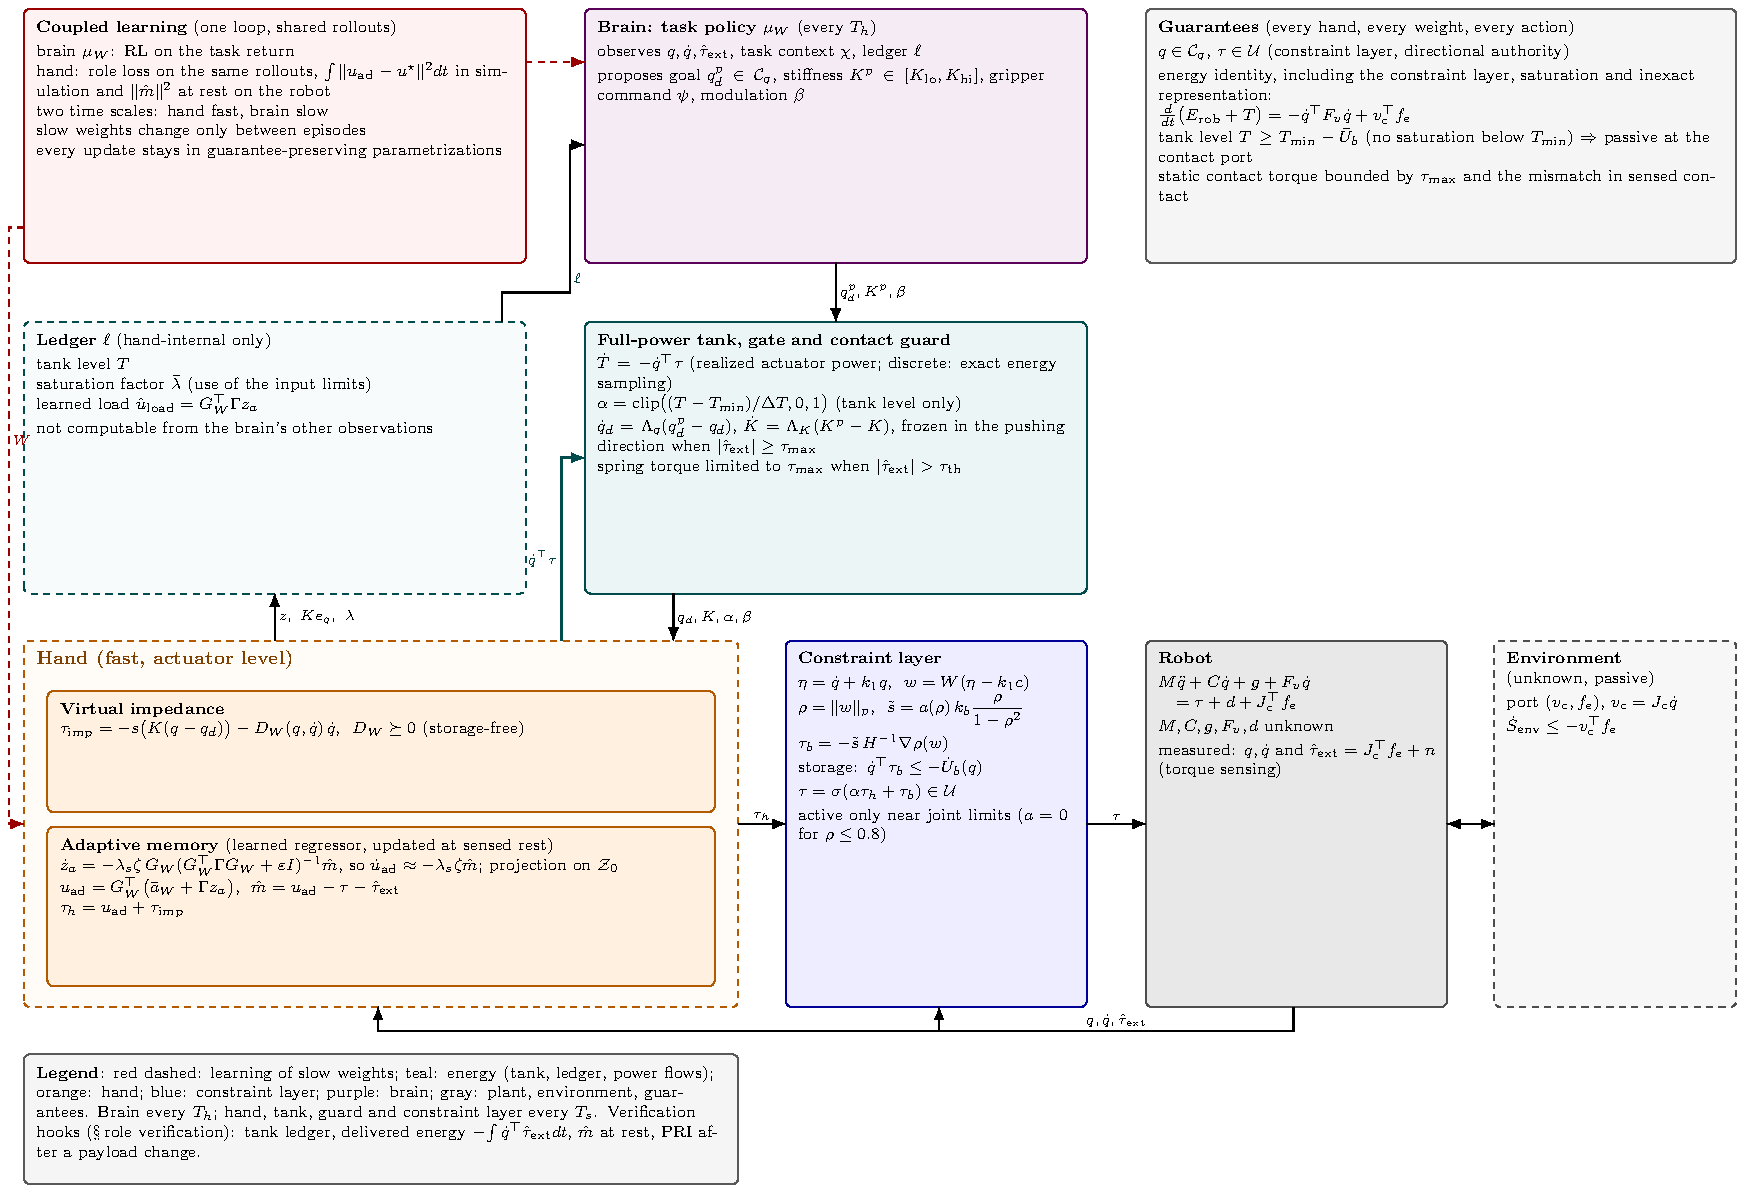
\includegraphics[width=\textheight]{architecture.pdf}
\caption{Architecture v3}
\label{fig:arch3}
\end{sidewaysfigure}

\section{이전 설계에서 배운 것}
\label{sec:lessons}

\textbf{두 설계의 결과.} 첫 설계는 적응 법칙 자체를 학습되는 port-Hamiltonian system으로 두고 궤적 추적에 썼다. 무작위 weight에서도 오차가 유계였고, 7-DOF manipulator에서 학습된 법칙의 추적 오차는 0.140--0.342 deg로 고gain 기준선(0.110--0.293 deg)에 가까웠으며, 기준선이 두 시험 집합에서 25\%와 38\% 발산하는 동안 발산하지 않았다. 둘째 설계(v2)는 task policy가 reference와 허용 오차를 제안하고 적응형 아래층이 양보하며 따르는 계층이었다. 제약 보장은 증명되었고 학습 중 위반도 없었지만, 같은 학습 예산에서 입력을 직접 내는 policy에 funnel filter를 붙인 기존 방식보다 관절 오차가 컸고(0.517--0.597 rad 대 0.289--0.307 rad), 사전 등록한 두 예측이 기각되어 중단되었다. 상세는 v2 사양, 제약 노트, 학습 비교 노트에 있다.

\textbf{교훈.}
\begin{enumerate}[label=(\arabic*)]
\item 안전을 reference 주변의 추종 tube로 얻으면, 경계에서 먼 곳에서도 운동이 느린 reference에 묶인다. 안전은 경계 근처에서만 개입해야 한다.
\item 보장을 "학습이 성능과 무관한 부분만 바꾸게 하는 것"으로 얻으면 학습할 것이 남지 않는다. 학습은 성능을 정하는 자유도(actuator 수준의 행동)에 닿아야 한다.
\item 양보가 자동으로 일어나면 위층의 최적 행동이 아래층의 상태와 무관해져, 보고가 쓰이지 않는다. 교환되는 지표는 받는 쪽의 결정을 바꿔야 한다.
\item 하나의 return으로 모든 parameter를 학습하면 역할이 정해지지 않는다. 역할에 맞는 신호로 학습한 feature가 단일 수리 중 가장 큰 효과를 냈다.
\item 점-대-점 도달 과제는 적응, passivity, 층의 결합 어느 것도 요구하지 않았다. 과제는 주장하는 이점을 실제로 요구해야 한다.
\end{enumerate}

\section{System과 과제}
\label{sec:system}

\begin{definition}[Robot and environment]
\label{def:robot}
\begin{itemize}
\item Robot: joint positions $q\in\R^m$, input torque $\tau\in\R^m$,
\[
M(q)\ddot q+C(q,\dot q)\dot q+g(q)+F_v\dot q=\tau+d+J_c(q)^\top f_e,
\]
with $M=M^\top$, $m_0I\preceq M(q)\preceq m_1I$ for known $0<m_0\le m_1$, $\dot M-2C$ skew-symmetric, $F_v=F_v^\top\succeq0$, and $M$, $C$, $g$, $F_v$ and the constant $d\in\R^m$ unknown; $(q,\dot q)$ is measured.
\item Contact port: $v_c:=J_c(q)\dot q\in\R^{n_c}$ and the force $f_e\in\R^{n_c}$ exerted by the environment on the robot.
\item Torque sensing: the external joint torque $\hat\tau_{\mathrm{ext}}:=J_c(q)^\top f_e+n$ is measured, from joint torque sensors or an end-effector force/torque sensor, with the weight of tool and payload removed by a tare at free-space rest and $\|n\|\le\bar n$.
\item Environment: a system with storage $S_{\mathrm{env}}\ge0$, unknown, that is \textbf{\emph{passive}} with respect to the contact port in the sense $\dot S_{\mathrm{env}}\le-v_c^\top f_e$.
\item Constraints: a box $\mathcal C_q:=\{q:\ |q_i-c_i|\le h_i\}$ of joint positions and the input box $\U:=\{\tau:\ |\tau_i|\le\bar u_i\}$.
\end{itemize}
\end{definition}

\begin{definition}[Task family]
\label{def:tasks}
\begin{itemize}
\item \textbf{Stage A} (one joint, $m=1$, $n_c=1$), used for component tests: a link under gravity with unknown payload starts at rest, reaches a wall at an unknown angle $q_w$ inside $\mathcal C_q$, presses on it with a target contact torque $\tau_c^\star$ and holds it. The wall is a spring-damper with unknown stiffness $k_e$ and damping $b_e$.
\item \textbf{Stage B} (three joints, $m=3$, $n_c=2$): the carry-and-press task of \Cref{def:stageBplant,def:stageBtask}.
\item \textbf{Stage C} (seven joints, $m=7$): defined after Stage B.
\item Reward: task terms only; no constraint, passivity or energy term.
\end{itemize}
\end{definition}

\textbf{직관 (단계의 역할).} Stage A는 부품의 기구를 빠르게 확인하는 시험대로만 쓴다. 한 관절에서는 뇌가 목표를 옮겨 부하를 흡수할 수 있어 적응의 필요를 시험하지 못하기 때문이다(\Cref{sec:m2audit}). 아이디어는 Stage B에서 시험하고, Stage C에서 7-DOF로 옮긴다.

\subsection{Stage B: 물체를 옮겨 누르는 평면 3관절 팔}
\label{sec:stageB}

\textbf{과제 (말로 된 설명).} 아래 각 항목은 \Cref{def:stageBplant}의 (a)--(e)와 \Cref{def:stageBtask}의 (f)--(l) 가운데 같은 표시의 항목과 같은 내용이다.
\begin{enumerate}[label=(\alph*)]
\item 로봇은 수직 평면에서 움직이는 3관절 팔이다. 관절 각도와 속도, 관절 공간의 외력 torque, 손끝 위치를 잰다. 팔의 질량, 관성, 마찰, 외란은 모른다.
\item 물체는 단단한 물체이고 알려진 위치에 잡는 점이 있다. 물체의 질량, 무게중심의 위치(잡는 점에서 8 cm 이내), 놓여 있는 방향은 모른다. 잡은 물체는 손끝에 단단히 붙어 팔의 일부로 함께 움직이고, 놓은 물체는 놓인 자리에 그대로 머문다. 처음 물체가 받침 위에 놓여 있는 것과 같은 추상화이며, 물체가 떨어지거나 다른 것과 부딪히는 일은 모형에 없다.
\item 잡기와 놓기는 뇌가 결정 시각마다 명령한다. 손끝이 잡는 점 가까이에 있고 모든 관절이 거의 멈춰 있을 때 잡기 명령을 내리면 물체가 손끝에 붙고, 그렇지 않으면 아무 일도 일어나지 않는다. 붙는 순간 물체는 제자리에 있고, 정지해 있던 물체와의 비탄성 충돌이어서 팔의 속도가 조금 줄어든다. 물체를 든 채 놓기 명령을 내리면 물체는 그 자리에 놓이고, 같은 조건에서 다시 잡을 수 있다. 로봇은 지금 물체를 들고 있는지와 놓은 물체의 잡는 점이 어디인지 안다.
\item 목표 위치 아래에 block이 있다. Block의 윗면 높이, 단단함, 소산, 마찰은 모른다. 손끝이 윗면을 누르면 위로 미는 힘과 옆으로 끄는 마찰력을 받고, 옆면을 누르면 옆으로 밀려난다. 힘은 닿는 순간 0에서 시작해 연속으로 변한다. 접촉은 손끝에서만 일어난다.
\item 감지된 외력에는 잡은 물체의 무게가 들어가지 않는다고 이상화한다. 잡거나 놓을 때마다 정지 상태에서 다시 하는 tare와 평면 손목 F/T sensor의 하중 식별에 해당하며, 사건 직후부터 첫 정지까지의 구간은 무시한 것이다. 감지에는 제어 한 주기의 지연, 작은 bias, 잡음이 있다.
\item 한 episode는 네 단계로 이어진다: 잡는 점으로 가서 잡기, 목표 위치로 옮겨 유지하기, 목표 위치 아래 block의 윗면을 목표 힘으로 누르기, 물체를 놓고 목표 위치로 물러나 유지하기. 각 단계의 길이는 무작위이다.
\item 뇌는 결정 시각마다 지금의 단계, 물체의 잡는 점의 현재 위치(들고 있으면 손끝), 목표 위치, 목표 힘, 잰 손끝 위치, 물체를 들고 있는지를 과제 정보로 받는다. Block은 목표 위치 바로 아래에 있다. 시간 자체는 받지 않는다.
\item 이 과제를 푸는 제어기는 \Cref{sec:arch}의 구조이고, 뇌는 결정 시각마다 목표 자세, 강성, 잡기 명령을 낸다.
\item 시작 자세는 관절 상자 안쪽에서 무작위이고, 팔은 멈춰 있으며, 물체를 들고 있지 않다. 손끝은 block의 윗면보다 높은 곳에서 시작하고, 잡는 점도 윗면보다 높다. 제어기의 내부 상태는 초기값에서 시작하고 기억은 비어 있다.
\item 전체 episode의 30\%에서는 가장 여유 있는 자세에서도 제약층이 작동하도록 관절 한계에 가까운 목표를 고르고, 나머지에서는 제약층이 작동하지 않는 자세가 있는 목표를 고른다. 이와 독립으로 30\%에서는 쓸 수 있는 에너지를, 정해진 기준 제어기가 같은 episode에서 쓴 에너지의 1.2--2배로 줄인다.
\item 비용은 episode 전체에 매긴다: 잡기 단계의 물체 잡는 점까지의 거리, 유지 단계의 손끝 위치 오차, 누르기 단계의 법선 힘 오차(닿기 전에는 block 윗면까지의 거리), 유지와 누르기 단계에서 물체를 놓쳤을 때의 벌점과 물체까지의 거리, 마지막 단계에서 물체를 놓지 못한 시간, 목표 힘의 두 배를 넘는 접촉 힘.
\item 성능은 각 단계의 마지막 40\%에서 잰 위치 오차와 힘 오차, 잡기 성공, 닿은 직후 0.3초 안의 최대 힘, 제약층과 gate가 작동한 시간의 비율, 최소 tank 수준으로 잰다.
\end{enumerate}

\begin{figure}[H]
\centering
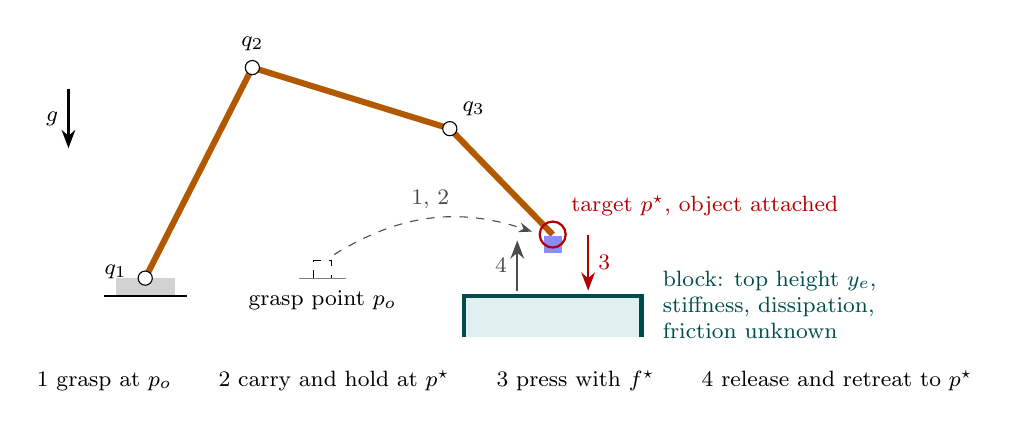
\begin{tikzpicture}[scale=7.5, >=Stealth, font=\footnotesize]
\coordinate (B) at (0,0); \coordinate (J1) at (0.1814,0.3565); \coordinate (J2) at (0.5158,0.2531); \coordinate (P) at (0.6900,0.0738);
\fill[gray!35] (-0.05,-0.03) rectangle (0.05,0); \draw[thick] (-0.07,-0.03) -- (0.07,-0.03);
\fill[teal!12] (0.54,-0.10) rectangle (0.84,-0.03); \draw[line width=1.6pt, teal!60!black] (0.54,-0.10) -- (0.54,-0.03) -- (0.84,-0.03) -- (0.84,-0.10);
\node[teal!60!black, right, align=left] at (0.86,-0.045) {block: top height $y_e$,\\ stiffness, dissipation,\\ friction unknown};
\draw[dashed] (0.285,0.0) rectangle (0.315,0.03); \draw[gray] (0.26,0.0) -- (0.34,0.0);
\node[below] at (0.30,-0.005) {grasp point $p_o$};
\draw[line width=2.2pt, orange!70!black] (B) -- (J1) -- (J2) -- (P);
\foreach \c in {B,J1,J2} \filldraw[fill=white, draw=black] (\c) circle (0.012);
\node[left] at ($(B)+(-0.015,0.01)$) {$q_1$}; \node[above] at ($(J1)+(0,0.012)$) {$q_2$}; \node[above right] at ($(J2)+(0.005,0.005)$) {$q_3$};
\fill[blue!45] ($(P)+(-0.015,-0.032)$) rectangle ($(P)+(0.015,-0.002)$);
\draw[red!70!black, thick] (P) circle (0.022);
\node[red!70!black, above right] at ($(P)+(0.015,0.015)$) {target $p^\star$, object attached};
\draw[->, dashed, gray!60!black] (0.32,0.04) to[bend left=25] node[pos=0.5, above] {1, 2} ($(P)+(-0.035,0.005)$);
\draw[->, thick, red!70!black] ($(P)+(0.06,0.0)$) -- ($(P)+(0.06,-0.095)$) node[pos=0.5, right] {3};
\draw[->, thick, gray!60!black] ($(P)+(-0.06,-0.095)$) -- ($(P)+(-0.06,-0.01)$) node[pos=0.5, left] {4};
\draw[->, thick] (-0.13,0.32) -- (-0.13,0.22) node[pos=0.5, left] {$g$};
\node[anchor=north west] at (-0.2,-0.14) {1 grasp at $p_o$\qquad 2 carry and hold at $p^\star$\qquad 3 press with $f^\star$\qquad 4 release and retreat to $p^\star$};
\end{tikzpicture}
\caption{Stage B task}
\label{fig:stageB}
\end{figure}

\begin{definition}[Stage B plant]
\label{def:stageBplant}
\begin{enumerate}[label=(\alph*)]
\item (Robot) An instance of \Cref{def:robot} with $m=3$: a planar serial arm with three revolute joints in a vertical plane under the gravitational acceleration $(0,-9.81)$ m/s$^2$, with link lengths $L_1,L_2,L_3>0$ and unknown link masses, inertias, $F_v$ and $d$. With $\vartheta_i:=\sum_{j\le i}q_j$, the tip position and its Jacobian are
\[
p(q):=\sum_{i=1}^{3}L_i\begin{bmatrix}\cos\vartheta_i\\ \sin\vartheta_i\end{bmatrix}\in\R^2,\qquad J_p(q):=\frac{\partial p}{\partial q}(q)\in\R^{2\times3}.
\]
The measured signals are $q$, $\dot q$, $\hat\tau_{\mathrm{ext}}\in\R^3$, the tip position $\hat p:=p(q)+n_p\in\R^2$ and the attachment state $\xi$ of (c).
\item (Object) A rigid body whose mass $m_{\mathrm{obj}}>0$ is concentrated at its center of mass $c\in\R^2$, with a unit vector $u\in\R^2$ fixed in the body and a material grasp point at distance $L_{\mathrm{obj}}\in[0,0.08]$ m from $c$; $m_{\mathrm{obj}}$, $L_{\mathrm{obj}}$ and $u(0)$ are unknown. The grasp point is
\[
o:=c+L_{\mathrm{obj}}\,u,\qquad o(0)=p_o\ \text{known}.
\]
While the object is detached ($\xi=0$), $(c,u)$ is constant. While it is attached ($\xi=1$), with the rotation $R(\vartheta_3)$ and $(r_{\mathrm{obj}},u_{\mathrm{rel}})$ fixed at the last grasp by (c),
\[
c=p(q)+R(\vartheta_3)\,r_{\mathrm{obj}},\qquad u=R(\vartheta_3)\,u_{\mathrm{rel}},
\]
and its mass is part of $M(q)$ and $g(q)$. For the task context and the cost, $o:=p(q)$ while attached.
\item (Gripper) The gripper command $\psi(t)\in\{0,1\}$ is piecewise constant and switches only at the decision times $t_k:=kT_h$, $T_h>0$. The grasp condition holds at $t_k$ iff
\[
\psi(t_k)=1,\qquad \|p(q)-o\|\le0.02\ \mathrm m,\qquad \|\dot q\|_\infty\le0.1\ \mathrm{rad/s}.
\]
The attachment state $\xi(t)\in\{0,1\}$, $\xi(0)=0$, changes only at the times $t_k$:
\[
\xi(t_k^+):=\begin{cases}1, & \xi(t_k^-)=0\ \text{and the grasp condition holds at }t_k,\\ 0, & \xi(t_k^-)=1\ \text{and}\ \psi(t_k)=0,\\ \xi(t_k^-), & \text{otherwise};\end{cases}
\]
A grasp keeps the pose of the object and fixes $r_{\mathrm{obj}}:=R(\vartheta_3)^\top\big(c-p(q)\big)$ and $u_{\mathrm{rel}}:=R(\vartheta_3)^\top u$, so that $\|r_{\mathrm{obj}}\|\le L_{\mathrm{obj}}+0.02$ m. With $M_-$ and $M_+$ the inertia matrices without and with the object, a grasp resets the velocity by conservation of the generalized momentum,
\[
\dot q(t_k^+):=M_+(q)^{-1}M_-(q)\,\dot q(t_k^-) ;
\]
a release leaves $\dot q$ unchanged, and the released object rests at its current pose and can be grasped again.
\item (Block) The block $\{(x,y):\ |x-x_e|<w_e,\ y<y_e\}$ has a center $x_e$ given by the task, a half-width $w_e$ and unknown top height $y_e$, stiffness $k_e$, dissipation $\delta_e$ and friction coefficient $\nu_e$. Only the tip makes contact, $J_c:=J_p$. With the depths $d_{\mathrm{top}}:=y_e-p_y$ and $d_{\mathrm{side}}:=w_e-|p_x-x_e|$, the tip is inside iff both are positive; outside, $f_e:=0$ and $f_n:=0$. Inside, on the top face ($d_{\mathrm{top}}\le d_{\mathrm{side}}$),
\[
f_n:=k_e\,d_{\mathrm{top}}\max\{0,\ 1-\delta_e\dot p_y\},\qquad f_e:=\begin{bmatrix}-\nu_ef_n\tanh\big(c_v\dot p_x/(\nu_ef_n)\big)\\ f_n\end{bmatrix},
\]
with $c_v=400$ N\,s/m and $f_e:=0$ when $f_n=0$, and on a side face ($d_{\mathrm{top}}>d_{\mathrm{side}}$), with $\varsigma:=\operatorname{sign}(p_x-x_e)$,
\[
f_s:=k_e\,d_{\mathrm{side}}\max\{0,\ 1-\delta_e\varsigma\dot p_x\},\qquad f_e:=\begin{bmatrix}\varsigma f_s\\ 0\end{bmatrix},\qquad f_n:=0 .
\]
\item (Sensing) $\hat\tau_{\mathrm{ext}}(t)=\big(J_p^\top f_e\big)(t-T_s)+b_\tau+n(t)$ with a constant bias $b_\tau$ and $\|n\|\le\bar n$; the attached object does not enter $\hat\tau_{\mathrm{ext}}$ (idealization).
\end{enumerate}
\end{definition}

\begin{fact}[Stage B plant and the plant class]
\label{fact:stageBclass}
\begin{enumerate}[label=(\alph*)]
\item The block is passive: with $S_{\mathrm{env}}:=\tfrac12k_e\min\{d_{\mathrm{top}},d_{\mathrm{side}}\}^2$ inside and $S_{\mathrm{env}}:=0$ outside, $\dot S_{\mathrm{env}}\le-v_c^\top f_e$.
\item Let $S_{\mathrm{obj}}:=(1-\xi)\,9.81\,m_{\mathrm{obj}}\,c_y$ be the potential energy of a resting object. At a grasp, $E_{\mathrm{rob}}+S_{\mathrm{obj}}$ does not increase. At a release, it decreases by the kinetic energy $\tfrac12m_{\mathrm{obj}}\|\dot c\|^2$ of the object.
\end{enumerate}
\end{fact}

\begin{proof}
(a) 윗면에서 깊이 $d=d_{\mathrm{top}}$, $\dot d=-\dot p_y$이고 마찰의 일률은 0 이하이다.
\[
\dot S_{\mathrm{env}}=k_ed\,\dot d,\qquad -v_c^\top f_e=\dot d\,f_n+\nu_ef_n\,\dot p_x\tanh\big(c_v\dot p_x/(\nu_ef_n)\big)\ \ge\ \dot d\,f_n .
\]
$1+\delta_e\dot d\ge0$이면 $\dot d\,f_n=k_ed\,\dot d+k_ed\,\delta_e\dot d^2\ge k_ed\,\dot d$이고, 그렇지 않으면 $f_n=0$, $\dot d<0$이어서 $0\ge k_ed\,\dot d$이다. 옆면도 같다. $S_{\mathrm{env}}$는 면 사이와 block의 경계에서 연속이다.

(b) 잡는 순간 $c$는 연속이고, $J_{\mathrm{obj}}:=\partial c/\partial q$(붙은 상태)에 대해 $M_+=M_-+m_{\mathrm{obj}}J_{\mathrm{obj}}^\top J_{\mathrm{obj}}\succeq M_-$이므로 $M_-^{1/2}M_+^{-1}M_-^{1/2}\preceq I$이다.
\[
\dot q(t_k^+)^\top M_+\dot q(t_k^+)=\dot q(t_k^-)^\top M_-M_+^{-1}M_-\dot q(t_k^-)\ \le\ \dot q(t_k^-)^\top M_-\dot q(t_k^-) .
\]
위치 에너지 $9.81\,m_{\mathrm{obj}}c_y$는 $S_{\mathrm{obj}}$에서 $E_{\mathrm{rob}}$으로 그대로 옮겨진다. 놓는 순간 $\dot q$와 $c$는 연속이고, $E_{\mathrm{rob}}$에서 물체의 운동 에너지 $\tfrac12m_{\mathrm{obj}}\|J_{\mathrm{obj}}\dot q\|^2$와 위치 에너지가 빠지며 위치 에너지만 $S_{\mathrm{obj}}$로 옮겨진다.
\end{proof}

\begin{definition}[Stage B task]
\label{def:stageBtask}
An episode of Stage B on the plant of \Cref{def:stageBplant} is specified as follows.
\begin{enumerate}[label=(\alph*), start=6]
\item (Phases) Durations $\Theta_1,\dots,\Theta_4>0$ define $\mathcal I_j:=\big[\sum_{i<j}\Theta_i,\ \sum_{i\le j}\Theta_i\big)$, $j=1,\dots,4$: pick ($\mathcal I_1$), carry and hold ($\mathcal I_2$), press ($\mathcal I_3$), release and retreat ($\mathcal I_4$). The episode ends at $\sum_{j}\Theta_j$.
\item (Task context) At each $t_k$ the controller receives
\[
\chi_k:=\big(\iota_k,\ o(t_k),\ p^\star,\ f^\star_{\mathrm{light}},\ f^\star_{\mathrm{heavy}},\ \hat p(t_k),\ \xi(t_k)\big)\in\{0,1\}^4\times\R^2\times\R^2\times\R_{>0}^2\times\R^2\times\{0,1\},
\]
where $\iota_k$ is the one-hot vector of the index $j$ with $t_k\in\mathcal I_j$, $o(t_k)$ is the grasp point of \Cref{def:stageBplant}(b), $p^\star\in\R^2$ is the target, and $f^\star_{\mathrm{light}}$, $f^\star_{\mathrm{heavy}}$ are the normal-force targets of the two payload classes. The target normal force is $f^\star:=f^\star_{\mathrm{heavy}}$ if $m_{\mathrm{obj}}>m_{\mathrm{th}}:=0.85$ kg and $f^\star:=f^\star_{\mathrm{light}}$ otherwise; $f^\star$ and $m_{\mathrm{obj}}$ are not part of $\chi_k$. The block center is $x_e:=p^\star_x$ with $y_e<p^\star_y$. No time input is given.
\item (Controller interface) The controller is the composed system of \Cref{sec:arch}; at each $t_k$ its brain issues $(q_d^p,K^p,\psi(t_k))$, with the modulation $\beta$ omitted.
\item (Initial state) $q(0)$ is uniform on $\{q:\ |q_i-c_i|\le0.6\,h_i,\ p_y(q)\ge y_e+0.03\ \mathrm m\}$, $\dot q(0)=0$, $\xi(0)=0$, and every controller state starts at its initial value with an empty adaptive memory.
\item (Hard episodes) With the gauge margin of a point,
\[
\operatorname{marg}(p):=1-\min_{q:\ p(q)=p}\big\|H^{-1}(q-c)\big\|_p ,
\]
the target satisfies $\operatorname{marg}(p^\star)\in[0.08,\,0.20)$ with probability $0.3$ and $\operatorname{marg}(p^\star)\ge0.25$ otherwise. In every episode $\operatorname{marg}(p_o)\ge0.25$, $\operatorname{marg}\big((p^\star_x,y_e)\big)\ge0.08$ and $p_{o,y}\ge y_e+0.03$ m. Independently, with probability $0.3$, the energy budget of the episode is $E_0:=\Delta T+\rho\,E_{\mathrm{task}}$ with $\rho$ uniform on $[0.6,1]$, where $E_{\mathrm{task}}:=\max_t\int_0^t\dot q^\top\tau\,ds$ along the run of the reference brain (\Cref{def:refbrain}) with the hand of \Cref{sec:arch} on the same episode with $E_0=E_{\mathrm{nom}}$; otherwise $E_0:=E_{\mathrm{nom}}$.
\item (Cost) The reward is $r_k:=-\int_{t_k}^{t_{k+1}}\Omega(t)\,dt$ with lengths in m and the cost rate
\[
\Omega:=\Omega_{\mathrm{task}}+5\max\{0,\ f_n-2f^\star\}/f^\star,
\]
\[
\Omega_{\mathrm{task}}:=\begin{cases}
\|p-o\|/0.1, & t\in\mathcal I_1,\\
\rho_j(o,\xi f_n)+(1-\xi)\big(1+\|p-o\|/0.1\big), & t\in\mathcal I_j,\ j\in\{2,3\},\\
\|p-p^\star\|/0.1+\xi, & t\in\mathcal I_4,
\end{cases}
\]
with the progress costs of the object at its grasp point $o$ under a top-face force $f\ge0$,
\[
\rho_2(o,f):=\|o-p^\star\|/0.1,\qquad \rho_3(o,f):=\Pi(o,f)+|o_x-p^\star_x|/0.1,
\]
\[
\Pi(o,f):=\begin{cases}\min\big\{\big((f-f^\star)/f^\star\big)^2,\ 1\big\}, & f>0,\\ 1+\|o-p_c\|/0.1, & f=0,\end{cases}\qquad p_c:=(p^\star_x,\,y_e)\in\R^2 .
\]
\item (Metrics) On the last 40\% of each phase, the position error $\|p-p^\star\|$ on $\mathcal I_2$ and $\mathcal I_4$ and the normal-force error $|f_n-f^\star|$ on $\mathcal I_3$; the grasp success $\xi=1$ at the end of $\mathcal I_1$; the class decision, correct if the mean of $f_n$ over the last 40\% of $\mathcal I_3$ is closer to $f^\star$ than to the other target; the peak of $f_n$ within 0.3 s after each contact onset; the fractions of time with constraint activity ($a>0$) and gate activity ($\alpha<1$); and $\min_tT(t)$.
\end{enumerate}
The distributions of the unknown quantities and the constants are in \Cref{tab:stageB}.
\end{definition}

\textbf{결정 (2026년 11월 14일).} 놓은 물체를 다시 잡을 수 있다. 그래서 물체를 자세 $(c,u)$를 가진 강체로 두고, 잡고 놓는 순간 물체가 움직이지 않게 했다. 이렇게 해야 사건에서 에너지가 생기지 않는다(\Cref{fact:stageBclass}(b)).

표의 $U[a,b]$는 균등 분포이다. Plant와 과제의 값은 설계 점검과 환경 검증으로 정했다(\Cref{sec:envcheck}). 제어기 상수는 L0에서 고정했다(\Cref{sec:l0}). $E_{\mathrm{nom}}$과 예산의 범위는 L1에서 정한다.

\begin{table}[H]
\centering\footnotesize
\caption{Stage B parameters}
\label{tab:stageB}
\begin{tabular}{p{3.9cm}p{6.2cm}p{4.6cm}}
\toprule
양 & 학습 분포 & 시험(분포 밖) \\
\midrule
링크 길이 $L_i$ [m] & $(0.40,0.35,0.25)$ & 각각 $\times[0.85,0.95]\cup[1.05,1.15]$ \\
링크 질량 [kg] & $(3.0,2.0,1.0)\times U[0.9,1.1]$ & 각각 $\times[0.7,0.9]\cup[1.1,1.3]$ \\
링크 관성 [kg\,m$^2$] & 질량$\times L_i^2/12$, 회전자 0.02 & 같음 \\
점성 마찰 $F_v$ [N\,m\,s/rad] & 대각, 성분별 $U[0.05,0.3]$ & 같음 \\
외란 $d$ [N\,m] & 성분별 $U[-0.5,0.5]$ & 같음 \\
물체 질량 $m_{\mathrm{obj}}$ [kg] & $[0.2,0.65]\cup[1.05,1.5]$에서 균등 & $U[1.5,2.5]$ \\
무게중심과 잡는 점의 거리 $L_{\mathrm{obj}}$ [m], 처음 방향 $u(0)$ & $U[0,0.08]$, 단위원 위에서 균등 & 같음 \\
$p_o$, $p^\star$ [m] & $[0.35,0.75]\times[-0.15,0.35]$에서 균등, (j)의 조건, $|p_{o,x}-p^\star_x|\ge0.2$ & 같음 \\
Block 윗면 높이 $y_e$ [m] & $p^\star_y-U[0.05,0.15]$ & 같음 \\
Block 강성 $k_e$ [N/m] & $\log$ 균등 $[2\cdot10^3,\,2\cdot10^4]$ & $2\cdot10^5$까지 \\
Block 소산 $\delta_e$ [s/m], 마찰 $\nu_e$ & $U[0.5,5]$, $U[0.2,0.8]$ & 같음 \\
등급별 목표 힘 $(f^\star_{\mathrm{light}},f^\star_{\mathrm{heavy}})$ [N] & $\{(f_1,f_2)\in[3,15]^2:\ |f_1-f_2|\ge4\}$에서 균등, 등급의 문턱 $m_{\mathrm{th}}=0.85$ kg & 같음 \\
예산 episode의 $\rho$ & $U[0.6,1]$ & 같음 \\
단계 길이 $\Theta_1,\dots,\Theta_4$ [s] & $U[1.5,2.5]$, $U[2,3]$, $U[2,3]$, $U[1.5,2.5]$ & 같음 \\
감지 잡음 & $n$ 성분별 표준편차 0.05 N\,m($\pm3$ 표준편차에서 절단), bias $b_\tau$ 성분별 $U[-0.05,0.05]$ N\,m, $n_p$ 0.002 m, $q$ 양자화 $10^{-4}$ rad, $\dot q$ 표준편차 0.01 rad/s & 같음 \\
plant 상수 & $\bar u=(120,60,25)$ N\,m, $c=(0.9,-1.3,-0.5)$ rad, $h=(0.9,1.1,1.2)$ rad, $w_e=0.15$ m, $E_{\mathrm{nom}}=60$ J & -- \\
제어기: 주기와 감지 & $T_h=50$ ms, $T_s=2$ ms, $\tau_{\mathrm{th}}=0.5$ N\,m, $\tau_{\max}=25$ N\,m & -- \\
제어기: 손 & {\raggedright $v_r=0.3$ rad/s, $t_r=0.1$ s, $\lambda_s=5$ s$^{-1}$, $\Gamma=I$, $\varepsilon=10^{-3}\operatorname{tr}(G_W^\top\Gamma G_W)/3$, $|z_i|\le50$, $\Lambda_q=20$ s$^{-1}$, $\Lambda_K=10$ s$^{-1}$, $k\in[(50,25,10),(400,200,80)]$ N\,m/rad, $K_n=(200,100,40)$ N\,m/rad, $D_W=\operatorname{diag}(30,12,2)$ N\,m\,s/rad\par} & -- \\
제어기: tank와 제약층 & $T_{\min}=1$ J, $\Delta T=1$ J, $k_1=2$, $k_b=2$, $p=8$, $\rho_{\mathrm{on}}=0.8$, $\rho_{\mathrm{full}}=0.9$ & -- \\
\bottomrule
\end{tabular}
\end{table}

\textbf{해석 (왜 이 과제인가).} 첫째, 한 과제에 두 종류의 일이 섞여 있고 나눌 수 있다. 어디로 가서 얼마나 세게 누를지는 과제마다 바뀌고 느리게 정해도 되는 의도이고, 모르는 무게 때문에 생기는 처짐은 목표와 무관하게 몸과 짐이 정하는 실행의 문제이다. 둘째, 적응이 필요하다. 물체 무게가 관절에 주는 torque는 자세마다 크기와 방향이 달라서, 뇌가 목표를 옮겨 맞추면 자세가 바뀔 때마다 다시 맞춰야 한다. 한 번의 정지 보정을 모든 자세로 옮기는 것은 학습된 regressor $G_W$의 몫이다. 셋째, 보장 장치가 실제로 작동한다. 단단한 block에서는 guard가, 한계 근처의 목표에서는 제약층이, 줄인 예산에서는 tank와 gate가 작동한다. 넷째, 누르는 힘의 목표가 물체 질량의 등급으로 정해지므로 뇌는 손이 배운 부하를 장부에서 읽어야 한다. 손이 보정을 마치면 처짐이 사라지고 감지된 외력에는 물체의 무게가 들어가지 않으므로, 뇌의 순간 관측에서 등급을 알 길은 장부뿐이다. 중복 자유도로 자세를 바꿔 예산을 아끼는 이득은 pilot에서 보이지 않았다(\Cref{sec:l1pilot}). 다섯째, 잡기와 놓기의 시각을 알기 때문에 그 직후의 뇌 반응으로 역할이 지켜졌는지 잴 수 있다. 감지의 이상화 (e)는, 평면 손목 F/T sensor에서 서로 다른 두 자세의 정지 측정이 물체의 질량과 무게중심의 위치를 정하므로, 잡을 때마다 그 측정을 한다고 가정한 것이다. 3차원에서는 더 많은 측정이 필요하므로 Stage C에서 다시 다룬다.


\begin{proposition}[Progress structure of the cost]
\label{prop:costprog}
Let $t\in\mathcal I_j$ with $j\in\{2,3\}$.
\begin{enumerate}[label=(\alph*)]
\item Let $\Omega^1_{\mathrm{task}}$ be the rate with the object held ($\xi=1$, $o=p$) and $\Omega^0_{\mathrm{task}}$ the rate with the object released at the same configuration ($\xi=0$, $o=p$), under the same tip force $f_n(t)$. If $j=2$ or $f_n(t)=0$, then $\Omega^0_{\mathrm{task}}-\Omega^1_{\mathrm{task}}=1$. If $j=3$ and $f_n(t)>0$, then $\Omega^0_{\mathrm{task}}-\Omega^1_{\mathrm{task}}\ge1$.
\item For $j=3$, $\xi=1$ and $f_n(t)=0$, the map $p\mapsto\Omega_{\mathrm{task}}=1+\|p-p_c\|/0.1+|p_x-p^\star_x|/0.1$ strictly decreases along the segment from every $p\ne p_c$ to $p_c$, and $p_c$ is its unique minimizer over $\R^2$.
\item For $j=3$, $\xi=1$ and a fixed $p$, the force part of the rate $g(f):=\Pi(p,f)+5\max\{0,f-2f^\star\}/f^\star$ is nonincreasing on $(0,f^\star]$ and nondecreasing on $[f^\star,\infty)$, and $f^\star$ is its unique minimizer over $f>0$, with $g(f^\star)=0$.
\end{enumerate}
\end{proposition}

\begin{proof}
(a) $o=p$를 정의에 넣는다. 놓은 상태에서는 $\xi f_n=0$이다.
\[
\Omega^1_{\mathrm{task}}=\rho_j(p,f_n),\qquad \Omega^0_{\mathrm{task}}=\rho_j(p,0)+1+\|p-p\|/0.1=\rho_j(p,0)+1
\]
$j=2$이면 $\rho_2$가 $f$에 의존하지 않고, $f_n=0$이면 두 $\rho_j$의 인자가 같으므로 차이는 1이다. $j=3$, $f_n>0$이면 다음과 같다.
\[
\Omega^0_{\mathrm{task}}-\Omega^1_{\mathrm{task}}=\Big(2+\frac{\|p-p_c\|}{0.1}+\frac{|p_x-p^\star_x|}{0.1}\Big)-\Big(\min\Big\{\Big(\frac{f_n-f^\star}{f^\star}\Big)^2,1\Big\}+\frac{|p_x-p^\star_x|}{0.1}\Big)\ge2-1=1
\]
(b) 선분 $p(s):=p+s(p_c-p)$, $s\in[0,1]$를 잡는다. $p_{c,x}=p^\star_x$이다.
\[
\|p(s)-p_c\|=(1-s)\,\|p-p_c\|
\]
\[
|p_x(s)-p^\star_x|=(1-s)\,|p_x-p^\star_x|
\]
\[
\Longrightarrow\quad \Omega_{\mathrm{task}}\big(p(s)\big)=1+(1-s)\big(\|p-p_c\|+|p_x-p^\star_x|\big)/0.1
\]
$p\ne p_c$이면 괄호 안이 양수이므로 $s$에 대해 strictly 감소한다. 또 $\Omega_{\mathrm{task}}\ge1$이고 등호는 $\|p-p_c\|=0$일 때만 성립한다.

(c) 구간을 나눈다.
\[
g(f)=\begin{cases}\big((f^\star-f)/f^\star\big)^2, & 0<f\le f^\star,\\ \big((f-f^\star)/f^\star\big)^2, & f^\star\le f\le 2f^\star,\\ 1+5\,(f-2f^\star)/f^\star, & f\ge 2f^\star.\end{cases}
\]
첫 구간에서 감소, 둘째 구간에서 0에서 1로 증가, 셋째 구간에서 1에서 증가하고, $f=2f^\star$에서 연속이다. $g(f^\star)=0$이고, $f\ne f^\star$이면 첫 두 구간에서 $g>0$, 셋째 구간에서 $g\ge1$이다.
\end{proof}

\textbf{해석 (학습 신호로서의 비용).} (a)에 의해 물체를 놓아도 물체의 진척 비용은 그대로 남고 1 이상이 더해지므로, 누르는 힘이 얼마이든 놓는 것이 비용을 낮추는 상태가 없다. (b)에 의해 접촉 전의 누르기 항은 어디서나 윗면 중심을 가리키므로, 기울기가 0인 영역이 없다. (c)에 의해 힘의 비용은 $f^\star$에서만 0이고 양쪽으로 멀어질수록 줄지 않는다. 상한 1 때문에 $2f^\star$ 위의 기울기는 과힘 항 $5\max\{0,f-2f^\star\}/f^\star$이 준다. 들고 있으면 $o=p$이므로 의도한 경로(잡고, $p^\star$로 옮기고, 바로 아래로 내려가 누르는 경로)의 비용은 개정 13과 같고, 힘이 $2f^\star$를 넘지 않으면 개정 14와도 같다. 개정 13은 (a)와 (b)를 어겼고, L2의 첫 시도에서 뇌가 그 결함을 그대로 학습했다(\Cref{sec:l2a1}). 개정 14는 힘이 있을 때 (a)를 어겼다(\Cref{fact:release14}). 세 성질은 환경 검증의 V17과 V18로 수치 확인한다(\Cref{sec:envcheck}).

\subsection{Stage B 환경: 설계 점검과 검증}
\label{sec:envcheck}

\textbf{직관 (환경이 틀리면 그 위의 결과가 모두 무의미하다).} 제어기를 올리기 전에 두 가지를 확인했다. 첫째, plant의 상수가 보장의 조건을 만족하는가. 둘째, 구현이 \Cref{def:stageBplant,def:stageBtask}와 같은가. 둘째는 서로 독립인 두 기준, 즉 SymPy로 유도한 Lagrange 방정식과 물리 engine MuJoCo에 대조했다. 합격 기준은 실행 전에 파일로 고정했다. 처음 두 번의 실행에서 결함 다섯 가지가 드러났고, 고칠 때마다 전체를 다시 돌려 세 번째 실행에서 모든 항목이 통과했다. 그 뒤 다시 잡기를 허용하도록 물체 모형을 바꾸고, 그에 맞게 시험을 고치거나 더해(V8, V10, V11, V16) 전체를 다시 돌렸으며, 새 시험의 결함 하나를 고쳐 한 번 더 돌렸다. 개정 14에서 비용의 정의를 바꾸면서 V11을 새 정의에 맞추고 비용의 성질을 재는 V17을 더해 여섯 번째로 돌렸다. 개정 15에서 누르기 항에 상한을 두면서 V11을 다시 맞추고 윗면 force가 있을 때의 성질을 재는 V18을 더해 일곱 번째로 돌렸다. 아래 값은 그 일곱 번째 실행의 것이다(\Cref{fig:envcheck}, \Cref{tab:envcheck}).

\begin{figure}[H]
\centering
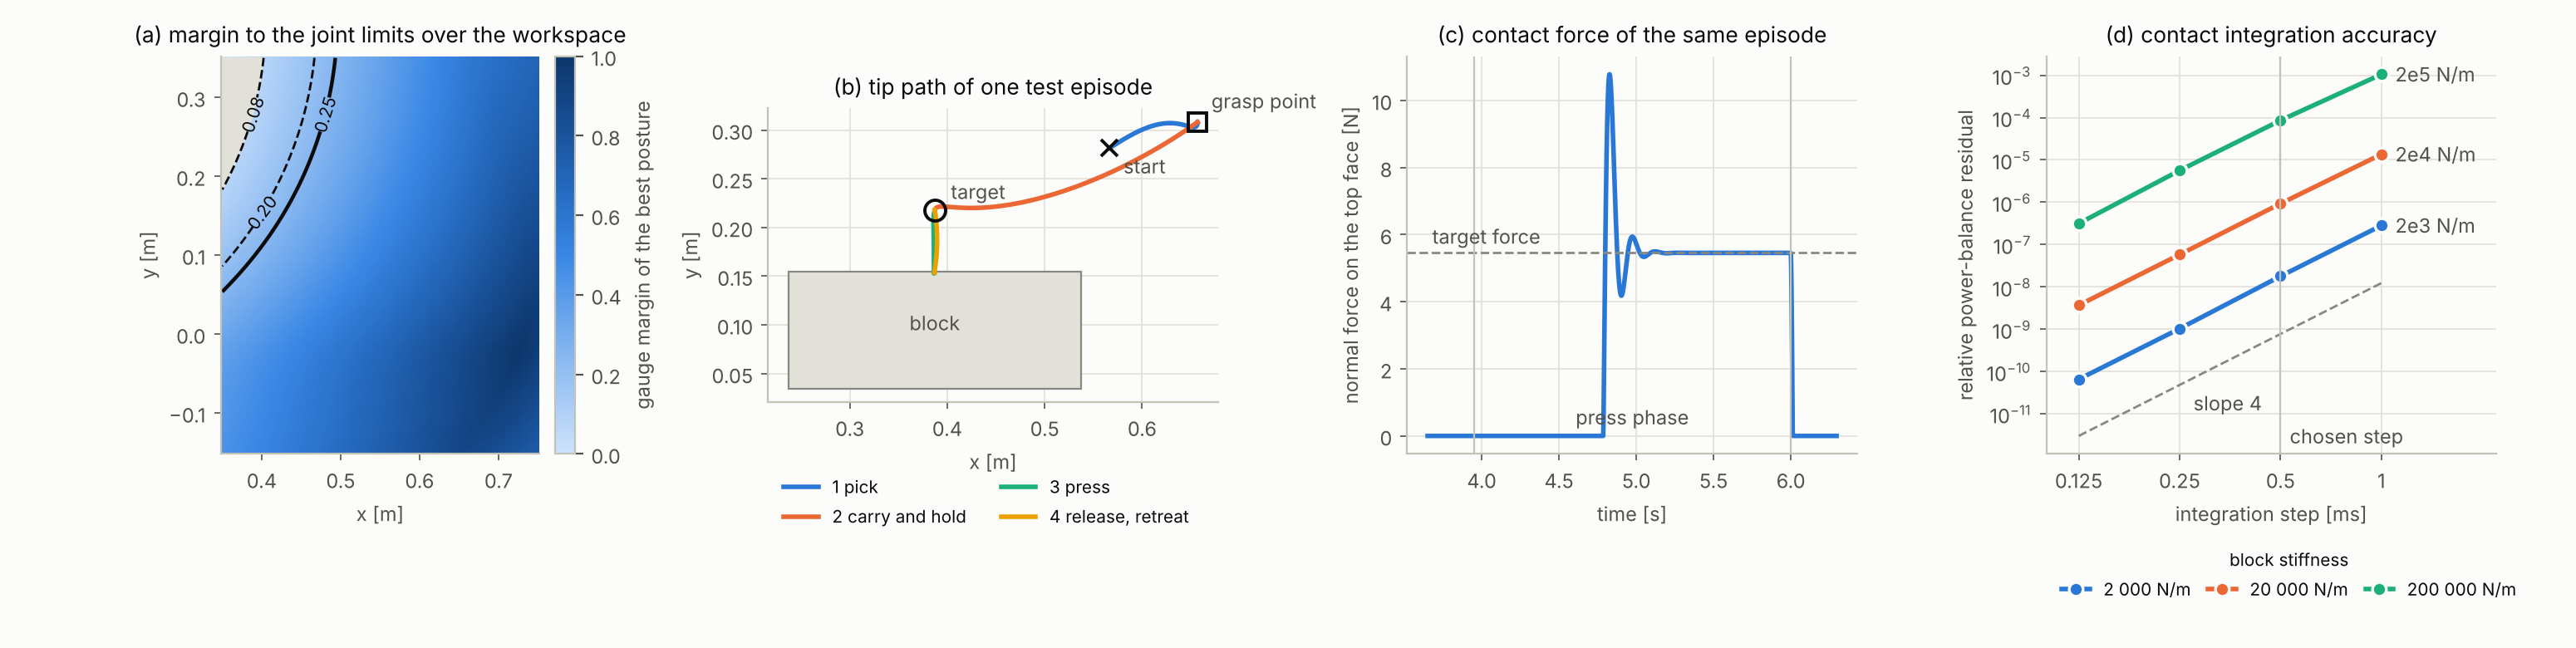
\includegraphics[width=\textwidth]{stageb_env.png}
\caption{Stage B environment checks}
\label{fig:envcheck}
\end{figure}

\textbf{설계 점검 (상수가 보장의 조건을 만족하는가).} \Cref{thm:r1}의 (B3)를 표본으로 확인했다. 표본은 집합 $\{\rho(w)=1,\ \rho(w_q)\le1\}$에서 경우마다 40{,}000개를 뽑았고, 붙은 물체의 offset은 $\|r_{\mathrm{obj}}\|\le0.10$ m에서, 접촉력은 마찰 원뿔($f_n\le60$ N, $\nu_e\le0.8$) 안에서 가장 불리한 값을 넣었다. 아래 값은 $k_1=2$에서 (B3)의 좌변에 음의 부호를 붙인 것의 최솟값이며, 양수이면 조건이 성립한다.
\[
\begin{array}{lcccc}
\bar u\ [\mathrm{N\,m}] & \text{in distribution} & \text{with contact} & \text{out of distribution} & \text{with contact}\\
(120,60,25) & 27.86 & 27.46 & 18.03 & 7.40\\
(80,40,15) & 10.97 & -70.39 & -4.68 & -95.57
\end{array}\quad\mathrm{rad/s^2}
\]
개정 9의 후보 $(80,40,15)$ N\,m는 접촉력이 걸리면 조건을 깨뜨렸다. 손목의 한계 15 N\,m가 60 N의 접촉력에 포화되기 때문이다. 그래서 $\bar u=(120,60,25)$ N\,m로 정했다. 이 확인은 표본에 대한 것이며 증명이 아니다. 관절 상자 $c=(0.9,-1.3,-0.5)$, $h=(0.9,1.1,1.2)$ rad에서 작업 영역의 85.7\%는 여유 0.25 이상의 자세가 있고, 7.3\%는 관절 한계에 가까운 띠 $[0.08,0.20)$에 있으며, 3.2\%는 닿지 않는다(\Cref{fig:envcheck}(a)). 가장 무거운 물체를 든 중력 torque는 입력 한계의 (0.37, 0.32, 0.28)배 이하(분포 안)와 (0.50, 0.51, 0.46)배 이하(분포 밖)이다.

\begin{table}[H]
\centering\footnotesize
\caption{Verification of the Stage B environment}
\label{tab:envcheck}
\begin{tabular}{p{0.6cm}p{5.8cm}p{4.9cm}p{3.5cm}}
\toprule
 & 확인한 것 & 측정값 & 기준(이하) \\
\midrule
V1 & 손끝 위치와 Jacobian (SymPy, MuJoCo 대조) & $3.2\cdot10^{-16}$, $2.9\cdot10^{-16}$ & $10^{-12}$, $10^{-9}$ \\
V2 & 관성 행렬 (SymPy, MuJoCo), 대칭 & $4.0\cdot10^{-16}$, $7.7\cdot10^{-13}$, $4.4\cdot10^{-16}$ & $10^{-12}$, $10^{-10}$, $10^{-12}$ \\
V3 & 관절 가속도 (SymPy, MuJoCo, 손끝 힘 포함) & $4.8\cdot10^{-15}$, $4.5\cdot10^{-11}$, $5.0\cdot10^{-11}$ & $10^{-10}$, $10^{-9}$, $10^{-9}$ \\
V4 & 중력 torque (SymPy, MuJoCo), 정지 유지의 가속도 & $7.9\cdot10^{-16}$, $1.8\cdot10^{-15}$, $5.2\cdot10^{-14}$ & $10^{-12}$, $10^{-10}$, $10^{-9}$ \\
V5 & 자유 운동의 에너지 drift(0.5 ms), 적분 차수 & $3.4\cdot10^{-8}$; 3.97, 3.98 & $10^{-7}$; $[3.5,4.5]$ \\
V6 & 접촉 없는 일률 균형의 잔차 & $1.4\cdot10^{-8}$ & $10^{-6}$ \\
V7 & 접촉: 구성한 힘 9개, 점별 passivity, 일률 균형($2\cdot10^4$ N/m, 0.5 ms) & $2.8\cdot10^{-13}$, $0$, $9.3\cdot10^{-7}$ & $10^{-9}$, $10^{-9}$, $10^{-4}$ \\
V8 & 잡기: 논리 11가지와 잡기--놓기--다시 잡기, 운동량 보존, 정지 잡기의 에너지와 무게중심 연속, 사건에서 $E_{\mathrm{rob}}+S_{\mathrm{obj}}$의 증가(무작위 2{,}000개) & 모두 일치, $1.6\cdot10^{-9}$, $6.7\cdot10^{-16}$, $0$, $0$ & 일치, $10^{-7}$, $10^{-9}$, $10^{-12}$, $10^{-9}$ \\
V9 & 감지: 한 주기 지연, 잡음 표준편차의 비, 양자화 오차 [rad] & $7.1\cdot10^{-15}$, 1.008--1.011, $5.0\cdot10^{-5}$ & $10^{-12}$, $1\pm0.02$, $0.5\cdot10^{-4}$ \\
V10 & 표본 추출: 3{,}000 episode에서 위반 수; 어려운 episode와 예산 episode의 비율; 분포 안 payload에서 무거운 등급의 비율 & 0; 0.298, 0.296; 0.510 & 0; $0.3\pm0.025$; $0.5\pm0.030$ \\
V11 & 비용: 구성한 상태 12개와 독립 계산의 차이 & $1.1\cdot10^{-16}$ & $10^{-9}$ \\
V12 & 묶음 실행과 단일 실행의 차이, 같은 seed의 재실행 & $7.1\cdot10^{-15}$, $0$ & $10^{-9}$, 0 \\
V13 & 단계 경계, 잡기 상태가 결정 시각에만 바뀌는지 & 일치 & 일치 \\
V14 & 전 구간(시험용 제어기, 64 episode): 에너지 감사의 잔차, 잡기 성공 & $3.3\cdot10^{-8}$, 64/64 & $10^{-4}$, 90\% \\
V15 & MuJoCo의 RK4와 1 s 궤적 차이 [rad] & $1.7\cdot10^{-8}$ & $10^{-6}$ \\
V16 & 다시 잡기(64 episode): 두 번 잡고 두 번 놓은 비율, 사건에서 $E_{\mathrm{rob}}+S_{\mathrm{obj}}$의 증가, 무게중심 연속, 에너지 감사의 잔차 & 100\%, $8.7\cdot10^{-16}$, $1.2\cdot10^{-16}$, $6.8\cdot10^{-8}$ & 90\%, $10^{-9}$, $10^{-12}$, $10^{-4}$ \\
V17 & 비용의 성질(무작위 자세 200{,}000개): 윗면 force가 없을 때 같은 자세에서 놓은 상태와 든 상태의 비용률 차이의 1로부터의 최대 편차; block 옆면을 따라 든 상태의 phase-3 비용률이 깊이에 대해 갖는 기울기 [1/m] & $5.3\cdot10^{-15}$; 6.37 & $10^{-9}$; $\ge1$ (이상) \\
V18 & 윗면 force가 있을 때의 비용의 성질(윗면 중심, 깊이 200개, 힘 $0.05f^\star$--$20f^\star$): 같은 자세에서 놓은 상태와 든 상태의 비용률 차이의 최솟값; 든 상태의 비용률이 가장 작은 곳의 $f/f^\star$ & 1.021; 0.985 & $\ge1$ (이상); 가장 가까운 깊이 \\
\bottomrule
\end{tabular}
\end{table}

오차는 최대 절대 차이를 (1 + 기준값의 최대 절댓값)으로 나눈 값이다. V1--V4는 상태 6{,}000개와 parameter 240벌(절반은 분포 밖의 몸, 절반은 물체를 든 상태)에서 쟀다. V16의 시험용 제어기는 목표 위치에서 물체를 놓고, 손끝 위치가 같은 다른 자세로 옮긴 뒤(마지막 링크 각도 변화의 중앙값 0.4 rad) 다시 잡는다.

\textbf{실행에서 드러난 결함과 수정.}
\begin{itemize}
\item Block 옆면의 감쇠 부호가 반대였다(코드의 오류). V7의 구성한 힘과 점별 passivity 확인이 잡았다.
\item Spring과 damper의 접촉 법칙은 닿는 순간 힘이 불연속이어서, 강성 $2\cdot10^4$ N/m에서 일률 균형의 잔차가 $8.5\cdot10^{-3}$이었다. 닿는 순간 힘이 0에서 시작하는 Hunt--Crossley 형태로 바꿨다. 그 뒤에도 잔차 $2.1\cdot10^{-3}$이 남았고, 원인은 다음 항목이었다.
\item 마찰의 정규화 $\tanh(\dot p_x/v_t)$는 속도 0에서의 기울기가 법선력에 비례해, 100 N이 넘는 충돌에서 적분의 안정 영역을 벗어났다. 기울기가 법선력과 무관하게 $c_v=400$ N\,s/m인 형태로 바꿨다. 그 뒤 잔차는 적분 간격의 4제곱으로 줄어든다(\Cref{fig:envcheck}(d)).
\item 시험용 제어기가 잡는 점으로 가는 길에 손끝이 block의 옆면을 지나갔다(최대 522 N). 잡는 점과 시작 위치를 block 윗면보다 0.03 m 이상 높게 뽑도록 했다.
\item 설계 점검 module을 불러오면 float64가 전역으로 켜지는 부작용이 있었다. NumPy만 쓰는 module로 분리했다.
\item 새 시험 V16의 에너지 감사가, 손끝이 잡는 점에서 1.31 cm 떨어진 자리에서 시작해 첫 결정 시각에 잡기가 일어난 episode(64개 중 1개)에서 사건 뒤의 에너지를 기준으로 삼았다(시험 코드의 오류, 잔차 0.058). 사건 전의 에너지를 기준으로 고쳤다.
\end{itemize}

\textbf{적분 간격의 선택.} Plant는 제어 주기 2 ms 안에서 4차 Runge--Kutta로 네 번 적분한다(0.5 ms). 이때 일률 균형의 잔차는 작동 영역(항상 누르는 접촉)에서 강성 $2\cdot10^5$ N/m까지 $1.7\cdot10^{-6}$ 이하이고, 떨어졌다가 다시 부딪히는 가혹한 영역에서 $2\cdot10^4$ N/m일 때 $9.3\cdot10^{-7}$, $2\cdot10^5$ N/m일 때 $8.6\cdot10^{-5}$이다. 그래서 학습 범위보다 단단한 block의 시험에서는 여덟 번 적분한다(같은 조건에서 $5.6\cdot10^{-6}$). 처리량은 float64에서 초당 제어 step 약 35{,}000개이고, float32로 돌린 궤적은 float64와 관절 각 $1.3\cdot10^{-1}$ rad, 법선력 2.4608 N(제곱 평균 제곱근) 이내로 일치했다.

\textbf{남은 한계.}
\begin{itemize}
\item (B3)의 확인은 표본에 대한 것이다.
\item 접촉은 penalty 모형이고 손끝에서만 일어난다. 링크와 block의 충돌, 물체의 충돌과 낙하는 없고, 놓은 물체는 놓인 자리에 머문다.
\item 잡는 순간 gauge는 최대 0.145만큼 뛸 수 있다(허용되는 잡기 상태 5{,}000개, 분포 밖의 몸 포함). \Cref{thm:r1}의 (B4)는 잡기 직전의 gauge가 0.855보다 작으면 성립한다.
\item 예산 episode의 예산 $E_0=\Delta T+\rho E_{\mathrm{task}}$에서 환경은 $\rho$를 뽑고, $E_{\mathrm{task}}$는 L1의 기준 뇌가 같은 episode에서 낸 값으로 환경 밖에서 정해 $E_0$을 episode의 parameter로 넘긴다.
\item 시험용 제어기는 중력 torque를 아는 PD와 힘 제어이며 v3의 구조가 아니다. \Cref{fig:envcheck}(c)의 닿는 순간 힘의 overshoot는 그 제어기의 것이다.
\end{itemize}

\section{준비: passivity와 port-Hamiltonian system}
\label{sec:prelim}

\textbf{직관 (에너지 장부).} Passivity는 system 안에 에너지원이 없다는 성질을 입출력으로 표현한 것이다. 저장된 에너지는 입출력 port로 들어온 일률만큼만 늘 수 있고, 나머지는 소산된다. 이 성질은 연결에 대해 닫혀 있어서, passive한 두 system을 음의 feedback으로 연결하면 두 storage의 합이 늘지 않는다. 고전 적응 제어의 안정성 증명은 이 연결의 한 예이다. 손의 적응 기억은 그 연결에서 적응 쪽 block을 학습되는 port-Hamiltonian system으로 바꾼 것이고(\Cref{lem:handbalance}), energy tank는 실제로 가한 일률을 지불해 그 연결의 passivity를 손의 구조와 무관하게 만든다(\Cref{lem:tank}).

\begin{definition}[Passivity]
\label{def:passive}
Consider a system with state $x\in\R^{n}$, input $u\in\R^{m}$ and output $y\in\R^{m}$,
\[
\dot x=f(x,u,t),\qquad y=h(x,u,t).
\]
\begin{itemize}
\item A \textbf{\emph{storage}} is a $C^1$ function $S:\R^n\to\R_{\ge0}$.
\item The system is \textbf{\emph{passive}} with storage $S$ if, along every solution and for every input,
\[
\dot S\le u^\top y .
\]
\item It is \textbf{\emph{lossless}} if equality holds, and \textbf{\emph{output strictly passive}} if $\exists\,\varepsilon>0$ with $\dot S\le u^\top y-\varepsilon\|y\|^2$.
\end{itemize}
\end{definition}

\begin{lemma}[Negative feedback interconnection]
\label{lem:interconnect}
Let $\Sigma_1$, $\Sigma_2$ be passive with storages $S_1$, $S_2$, inputs $u_1,u_2\in\R^m$ and outputs $y_1,y_2\in\R^m$, connected by $u_1=-y_2$ and $u_2=y_1$. Then $S_1+S_2$ is nonincreasing along every solution of the interconnection.
\end{lemma}

\begin{proof}
두 부등식을 더한다.
\[
\dot S_1+\dot S_2\le u_1^\top y_1+u_2^\top y_2 .
\]
연결식을 넣는다.
\[
u_1^\top y_1+u_2^\top y_2=-y_2^\top y_1+y_1^\top y_2=0 .
\]
\end{proof}

\begin{definition}[Port-Hamiltonian system]
\label{def:ph}
A \textbf{\emph{port-Hamiltonian system}} with state $z\in\R^{n}$ and port $(u,y)\in\R^m\times\R^m$ is
\[
\dot z=\big(\mathcal J(z,t)-\mathcal R(z,t)\big)\nabla H(z)+\mathcal G(z,t)\,u,\qquad y=\mathcal G(z,t)^\top\nabla H(z),
\]
where
\begin{itemize}
\item the \textbf{\emph{Hamiltonian}} $H:\R^n\to\R$ is $C^1$ and bounded from below;
\item the \textbf{\emph{interconnection}} $\mathcal J(z,t)\in\R^{n\times n}$ satisfies $\mathcal J=-\mathcal J^\top$;
\item the \textbf{\emph{dissipation}} $\mathcal R(z,t)\in\R^{n\times n}$ satisfies $\mathcal R=\mathcal R^\top\succeq0$;
\item the \textbf{\emph{port matrix}} is $\mathcal G(z,t)\in\R^{n\times m}$.
\end{itemize}
\end{definition}

\begin{lemma}[Port-Hamiltonian systems are passive]
\label{lem:phpassive}
For every $\mathcal J$, $\mathcal R$, $\mathcal G$ satisfying the conditions of \Cref{def:ph}, including time-varying ones,
\[
\dot H=-\nabla H^\top\mathcal R\,\nabla H+u^\top y\le u^\top y ,
\]
so the system is passive with storage $H-\inf H$.
\end{lemma}

\begin{proof}
해를 $z(t)$로 두고, 각 시각의 gradient를 벡터 하나로 부른다.
\[
v(t):=\nabla H\big(z(t)\big)\in\R^n .
\]
$H\in C^1$이고 $z(t)$가 미분 가능한 시각에서 연쇄 법칙이 성립한다.
\[
\frac{d}{dt}H\big(z(t)\big)=v^\top\dot z .
\]
$\dot z$에 \Cref{def:ph}의 우변을 넣는다. 우변이 $\nabla H$로 만들어져 있으므로 결과는 $v$만의 식이다.
\[
\dot H=v^\top\mathcal J\,v-v^\top\mathcal R\,v+v^\top\mathcal G\,u .
\]
세 항을 각각 정리한다. 각 단계는 $v$가 어떤 벡터이든 성립하므로 $H$의 구체적인 형태를 쓰지 않는다. 첫째 항은 scalar가 자기 transpose와 같다는 것과 $\mathcal J^\top=-\mathcal J$에서 0이다.
\[
v^\top\mathcal J\,v=\big(v^\top\mathcal J\,v\big)^\top=v^\top\mathcal J^\top v=-v^\top\mathcal J\,v\ \Longrightarrow\ v^\top\mathcal J\,v=0 .
\]
둘째 항은 $\mathcal R$의 정의에서 0 이상이다.
\[
\mathcal R\succeq0\ \Longrightarrow\ v^\top\mathcal R\,v\ge0 .
\]
셋째 항은 출력의 정의이다.
\[
v^\top\mathcal G\,u=\big(\mathcal G^\top v\big)^\top u=y^\top u .
\]
\end{proof}

\begin{remark}[Why no formula for $H$ is needed]
\label{rem:noformula}
일반적인 ODE $\dot z=f(z)$에서는 $\dot H=\nabla H^\top f$가 $H$와 $f$ 모두에 의존한다. Port-Hamiltonian system에서는 vector field 자체를 $\nabla H$로 만들기 때문에, $\dot H$가 $\nabla H$의 2차식과 port 항으로 바뀌고 그 부호는 $\mathcal J$와 $\mathcal R$의 구조만으로 정해진다. 기하적으로 $\mathcal J\nabla H$는 $\nabla H$와 직교하므로 $H$의 등위면을 따라 움직이고, $-\mathcal R\nabla H$는 $H$가 줄어드는 방향이다.
\[
\nabla H^\top\big(\mathcal J\nabla H\big)=0,\qquad \nabla H^\top\big(-\mathcal R\nabla H\big)\le0 .
\]
2차 Hamiltonian $H(z)=\tfrac12z^\top Qz$($Q\succ0$)에서는 $\nabla H=Qz$이고, 같은 계산이 다음과 같다.
\[
\dot z=(\mathcal J-\mathcal R)Qz+\mathcal Gu,\qquad \dot H=z^\top Q\dot z=-(Qz)^\top\mathcal R\,(Qz)+(\mathcal G^\top Qz)^\top u .
\]
계산에 쓰인 $H$의 성질은 $C^1$뿐이다. Bounded below는 $H-\inf H\ge0$을 storage로 쓰기 위해서만 필요하고, 해의 존재는 $\nabla H$가 locally Lipschitz일 때 보장된다.
\end{remark}

\textbf{직관 (이름과 세 구조).} 이름의 Hamiltonian은 해석역학에서 운동이 에너지 함수의 gradient와 skew 구조로 생성된다는 것($\dot z=\mathcal J\nabla H$이면 $H$가 보존된다)에서, port는 곱이 일률이 되는 입출력 쌍에서 왔다(Maschke와 van der Schaft, 1992). $\mathcal J$는 상태 사이에서 에너지를 옮기기만 하고, $\mathcal R$은 없애기만 하며, $\mathcal G$는 port를 통한 출입만 담당한다. 세 역할이 분리되어 있으므로 $H$, $\mathcal J$, $\mathcal R$, $\mathcal G$를 어떤 network로 두어도 \Cref{lem:phpassive}가 성립한다.

\begin{remark}[Two instances]
\label{rem:phex}
적분기는 $H(z)=\tfrac12\|z\|^2$, $\mathcal J=\mathcal R=0$, $\mathcal G=I$인 경우이다.
\[
\dot z=u,\qquad y=z,\qquad \dot H=u^\top y .
\]
상태가 $z\in\R^2$이고 $H(z)=\tfrac12\|z\|^2$일 때, 다음 구조는 감쇠 $\rho\ge0$를 가진 각진동수 $\omega$의 진동자를 준다.
\[
\mathcal J=\begin{pmatrix}0&\omega\\-\omega&0\end{pmatrix},\qquad \mathcal R=\begin{pmatrix}0&0\\0&\rho\end{pmatrix}\quad\Longrightarrow\quad \dot z_1=\omega z_2+(\mathcal Gu)_1,\quad \dot z_2=-\omega z_1-\rho z_2+(\mathcal Gu)_2 .
\]
\end{remark}

\subsection{Energy tank}
\label{sec:tankdef}

\textbf{직관 (지불 장치).} 강성을 바꾸거나 목표를 옮기는 요구는 가상 spring에 에너지를 주입하고, 그만큼 controller가 passivity를 잃을 수 있다. Energy tank는 controller가 소산한 에너지를 저장했다가 그런 요구를 지불하는 데 쓰는 가상 저장소이다. 요구를 tank가 지불할 수 있을 때만 실행하면, tank를 포함한 전체가 passive하게 남는다.

\begin{definition}[Energy tank]
\label{def:tank}
An \textbf{\emph{energy tank}} has state $x_T\in\R_{>0}$, energy $T:=\tfrac12x_T^2$, constants $0<T_{\min}<T_{\max}$, and dynamics
\[
\dot x_T=\frac{1}{x_T}\big(\phi\,P_{\mathrm{diss}}-P_{\mathrm{dem}}\big),\qquad \phi:=\begin{cases}1,&T<T_{\max},\\0,&T\ge T_{\max},\end{cases}
\]
driven by a supplied power $P_{\mathrm{diss}}\ge0$ and a demanded power $P_{\mathrm{dem}}\in\R$, so that $\dot T=\phi\,P_{\mathrm{diss}}-P_{\mathrm{dem}}$.
\end{definition}

\begin{lemma}[Tank-augmented passivity]
\label{lem:tank}
Let a system with storage $E\ge0$ and port $(v,f)\in\R^{n}\times\R^{n}$ satisfy
\[
\dot E\le-P_{\mathrm{diss}}+P_{\mathrm{dem}}+v^\top f
\]
with $P_{\mathrm{diss}}\ge0$. Then, with the tank of \Cref{def:tank} driven by the same $P_{\mathrm{diss}}$ and $P_{\mathrm{dem}}$,
\[
\frac{d}{dt}\big(E+T\big)\le-(1-\phi)\,P_{\mathrm{diss}}+v^\top f\le v^\top f .
\]
\end{lemma}

\begin{proof}
두 변화율을 더한다.
\[
\dot E+\dot T\le-P_{\mathrm{diss}}+P_{\mathrm{dem}}+v^\top f+\phi\,P_{\mathrm{diss}}-P_{\mathrm{dem}} .
\]
$0\le\phi\le1$이고 $P_{\mathrm{diss}}\ge0$이다.
\end{proof}

\section{구조}
\label{sec:arch}

\textbf{직관 (네 부분).} 손은 뇌가 정한 목표와 강성을 가진 가상 spring과 damper를 구현하고, 정지 상태마다 감지된 torque로 미지의 중력과 외란을 적응 기억에 배운다. Energy tank는 손과 제약층이 실제로 가한 torque의 일률을 지불하므로 접촉 port의 passivity는 손의 구조와 무관하게 성립하고, 접촉 guard는 감지된 접촉 torque로 목표와 강성의 전진을 멈추고, 손은 감지된 접촉에서 spring torque를 제한한다. 제약층은 관절 한계 근처에서만 복원 torque를 더한다. 뇌는 목표, 강성, 잡기를 고르고, 손만 아는 상태(남은 예산, 능력 사용, 배운 부하)를 장부로 본다.

\subsection{손: 가상 impedance와 적응 기억}

\begin{definition}[Hand]
\label{def:hand}
Given the realized goal $q_d\in\mathcal C_q$ and stiffness $K=\operatorname{diag}(k)$, $k\in[k_{\mathrm{lo}},k_{\mathrm{hi}}]^m$, with $e_q:=q-q_d\in\R^m$, the \textbf{\emph{hand}} outputs
\[
\tau_h:=u_{\mathrm{ad}}-s\big(K\,e_q\big)-D_W(q,\dot q)\,\dot q\in\R^m,
\]
where
\begin{itemize}
\item the spring torque is limited in sensed contact: $s(v):=v$ if $\|\hat\tau_{\mathrm{ext}}\|\le\tau_{\mathrm{th}}$ and $s(v):=v/\max\{1,\|v\|/\tau_{\max}\}$ otherwise, with a contact threshold $\tau_{\mathrm{th}}>\bar n$ and a limit $\tau_{\max}>\tau_{\mathrm{th}}$;
\item the damping $D_W(q,\dot q)\in\R^{m\times m}$, $D_W=D_W^\top\succeq0$, is a network (storage-free), selected by the modulation $\beta$ of the brain;
\item the \textbf{\emph{adaptive memory}} has fast weights $z_a\in\R^{n_a}$, a feature network $G_W(q)\in\R^{n_a\times m}$, a prior $\bar a_W\in\R^{n_a}$ and a gain $\Gamma=\Gamma^\top\succ0$, with output and update
\[
u_{\mathrm{ad}}:=G_W(q)^\top\big(\bar a_W+\Gamma z_a\big),\qquad \dot z_a=-\lambda_s\,\zeta\,G_W(q)\big(G_W(q)^\top\Gamma\,G_W(q)+\varepsilon I\big)^{-1}\hat m,
\]
followed by a projection onto a compact set $\mathcal Z_0\subset\R^{n_a}$, with $\lambda_s>0$ and a regularization $\varepsilon>0$;
\item the \textbf{\emph{measured mismatch}} is $\hat m:=u_{\mathrm{ad}}-\tau-\hat\tau_{\mathrm{ext}}\in\R^m$ with the applied input torque $\tau$;
\item the \textbf{\emph{rest indicator}} is $\zeta(t):=1$ if $\|\dot q(s)\|_\infty\le v_r$ $\forall s\in[t-t_r,t]$, and $\zeta(t):=0$ otherwise, with $v_r>0$ and $t_r>0$.
\end{itemize}
With $u^\star:=g-d$, the representation is \textbf{\emph{exact}} if $\exists\,c^\star\in\R^{n_a}$ with $u^\star(q)=G_W(q)^\top c^\star$ on $\mathcal C_q$.
\end{definition}

\begin{fact}[Measured mismatch]
\label{fact:mhat}
Along every solution,
\[
\hat m=\big(u_{\mathrm{ad}}-u^\star\big)-M(q)\ddot q-C(q,\dot q)\dot q-F_v\dot q-n .
\]
In particular, $\dot q=0$ and $\ddot q=0$ $\Rightarrow$ $\hat m=u_{\mathrm{ad}}-u^\star-n$. If $\tau=\tau_h$ (gate open, constraint layer and saturation inactive), then $\hat m=s(Ke_q)+D_W\dot q-\hat\tau_{\mathrm{ext}}$; in free space this is $Ke_q+D_W\dot q-n$.
\end{fact}

\begin{proof}
운동 방정식(\Cref{def:robot})에서 가한 torque를 푼다.
\[
\tau=M\ddot q+C\dot q+g+F_v\dot q-d-J_c^\top f_e .
\]
$\hat\tau_{\mathrm{ext}}=J_c^\top f_e+n$을 $\hat m$의 정의에 넣으면 접촉 항이 상쇄된다. 둘째 식은 $\tau_h$의 정의를 $\hat m$에 넣은 것이다.
\end{proof}

\textbf{해석 (정지 상태에서만 배우는 이유).} 운동 중에는 $\hat m$에 관성, Coriolis, 마찰 torque가 섞이므로(\Cref{fact:mhat}), 기억은 rest indicator가 켜진 동안만 갱신된다. 갱신은 정규화되어 있어서, 자세가 고정되고 $z_a$가 $\mathcal Z_0$ 안에 있으면 $\dot u_{\mathrm{ad}}=-\lambda_s\zeta\,G_W^\top\Gamma G_W(G_W^\top\Gamma G_W+\varepsilon I)^{-1}\hat m$이고, $G_W$의 rank가 $m$이면 $\varepsilon\to0$에서 $-\lambda_s\zeta\hat m$이다. 그래서 정지 상태의 보정 속도와 안정성은 학습된 feature와 무관하고, $G_W$는 한 자세의 보정이 다른 자세로 옮겨 가는 방식만 정한다. 정규화하지 않은 gradient 법칙은 $G_W^\top G_W$가 관절 사이를 결합해 L0에서 진동했다(\Cref{sec:l0}). Projection이 $z_a$를 유계로 둔다. 자유 공간에서는 둘째 식에 의해 impedance 오차 $Ke_q$에 대한 적분 동작과 같다. $v_r=0.3$ rad/s는 엄밀한 정지가 아니라 느린 운동이며, 이때 점성 마찰 항은 성분별 0.09 N\,m 이하이다. 속도로 구동되던 개정 7까지의 port-Hamiltonian 기억은 M2 점검에서 치우침의 경로로 확인되어 대체되었다(\Cref{sec:m2audit,app:oldmem}).

\subsection{Full-power tank과 접촉 guard}
\label{sec:tank3}

\begin{definition}[Full-power tank]
\label{def:fulltank}
The tank pays the realized actuator power and gates the hand torque by its level:
\[
\dot T=-\dot q^\top\tau,\qquad \tau=\sigma\big(\alpha\,\tau_h+\tau_b\big),\qquad \alpha:=\min\big\{1,\max\{0,(T-T_{\min})/\Delta T\}\big\},
\]
with the initial level $T(0):=T_{\min}+E_0$ for the energy budget $E_0>0$ of the episode.
\end{definition}

\begin{theorem}[Passivity for every hand]
\label{thm:fulltank}
Let $V_g(q)$ be the potential of gravity ($\nabla V_g=g$) and $E_{\mathrm{rob}}:=\tfrac12\dot q^\top M\dot q+V_g(q)-d^\top q$. For every hand torque $\tau_h$, every weight and every proposal:
\begin{enumerate}[label=(\alph*)]
\item (Energy identity) on every interval without events,
\[
\frac{d}{dt}\big(E_{\mathrm{rob}}+T\big)=-\dot q^\top F_v\dot q+v_c^\top f_e ;
\]
\item (Tank level) if the saturation is inactive whenever $T<T_{\min}$, then
\[
T(t)\ \ge\ T_{\min}-\sup_{s\le t}U_b\big(q(s)\big)\qquad\forall t\ge0 ;
\]
\item (Passivity) under (b) and with a constant $\bar U_b\ge\sup_tU_b(q(t))$, the function $S:=E_{\mathrm{rob}}-\inf E_{\mathrm{rob}}+T-T_{\min}+\bar U_b\ge0$ satisfies $\dot S\le v_c^\top f_e$ on every interval without events.
\end{enumerate}
No exact representation is assumed, and the active constraint layer is included. Under the conditions of \Cref{thm:r1}, $\bar U_b:=\Psi\big(\max\{\rho(w_q(0)),\rho(w(0)),\bar\rho\}\big)<\infty$.
\end{theorem}

\begin{proof}
(a) 운동 방정식에서 다음을 얻고 $\dot T=-\dot q^\top\tau$를 더한다.
\[
\frac{d}{dt}E_{\mathrm{rob}}=\dot q^\top\big(\tau-F_v\dot q+J_c^\top f_e\big) .
\]
(b) $T(t)<T_{\min}$인 $t$에 대해 $t_1:=\sup\{s\le t:\ T(s)\ge T_{\min}\}$로 두면 $T(t_1)=T_{\min}$이다. $(t_1,t]$에서 $T<T_{\min}$이므로 $\alpha=0$이고, saturation이 없으므로 $\tau=\tau_b$이다. \Cref{lem:barrier}를 쓴다.
\[
\dot T=-\dot q^\top\tau_b\ \ge\ \frac{d}{dt}U_b(q)
\]
\[
\Longrightarrow\quad T(t)\ge T_{\min}+U_b\big(q(t)\big)-U_b\big(q(t_1)\big)\ge T_{\min}-U_b\big(q(t_1)\big) .
\]
(c) (a)와 (b)에서 바로 나온다.
\end{proof}

\textbf{해석 (gate가 걸리는 곳과 걸리지 않는 곳).} Gate는 손에만 걸리고 제약층에는 걸리지 않는다. 제약층을 gate로 막으면 관절 제약의 보장(\Cref{thm:r1})이 깨지기 때문이다. Gate는 tank 수준에만 의존하므로 tank가 비면 손의 감쇠 $-D_W\dot q$도 함께 꺼지고, 남는 감쇠는 점성 마찰과 제약층뿐이다. 손의 일률이 음이면 통과시키던 예외 규칙은 이산 시간에서 tank를 $T_{\min}$ 아래로 새게 해 L0에서 없앴다(\Cref{sec:l0}). 그 대신 제약층이 tank에서 꺼낼 수 있는 에너지는 저장 함수 $U_b$로 제한되고, 그 상한 $\bar U_b$가 passivity의 저장 함수에 상수로 더해진다. $T<T_{\min}$인 동안 saturation이 작동하는 경우는 다루지 못했다. 그때 하한은 $U_b(q(\cdot))$의 감소량의 합으로 바뀌며, 이것이 유계인지는 미해결이다 (R7). 잡기와 놓기의 순간에 $E_{\mathrm{rob}}$이 어떻게 뛰는지는 \Cref{fact:stageBclass}에 있다.

\textbf{해석 (무엇이 단순해지나).} \Cref{thm:fulltank}의 항등식은 손의 내부 구조와 무관하다. 그래서 부정확한 표현 (R11)이 같은 계산에 포함되고, 기억은 passivity를 깨지 않고 측정된 mismatch로 갱신될 수 있다. 대가는 tank가 중력에 대한 일까지 지불하므로 예산에 위치 에너지의 변화가 들어간다는 것이다.

\begin{definition}[Contact guard]
\label{def:guard}
The realized goal and stiffness move toward the proposal, $\dot q_d=\Lambda_q(q_d^p-q_d)$ and $\dot K=\Lambda_K(K^p-K)$ with diagonal $\Lambda_q,\Lambda_K\succ0$, except that, while $\|\hat\tau_{\mathrm{ext}}\|\ge\tau_{\max}$, $\dot q_d:=0$ and $\dot K:=0$ whenever the proposed update increases the spring torque, i.e. $(Ke_q)^\top\big(\dot K e_q-K\dot q_d\big)>0$.
\end{definition}

\begin{proposition}[Static contact torque bound]
\label{prop:static}
Let the projection keep $\|u_{\mathrm{ad}}\|\le\bar u_{\mathrm{ad}}$ and let $\|u^\star\|\le\bar u^\star$ on $\mathcal C_q$. At every rest state with $q,q_d\in\mathcal C_q$, $\alpha=1$ and the constraint layer and the saturation inactive:
\begin{enumerate}[label=(\alph*)]
\item $\big\|J_c^\top f_e\big\|\le k_{\mathrm{hi}}\,\operatorname{diam}(\mathcal C_q)+\bar u_{\mathrm{ad}}+\bar u^\star$;
\item if $\|\hat\tau_{\mathrm{ext}}\|>\tau_{\mathrm{th}}$, then $\big\|J_c^\top f_e\big\|\le\tau_{\max}+\|u_{\mathrm{ad}}-u^\star\|$.
\end{enumerate}
\end{proposition}

\begin{proof}
정지 상태의 운동 방정식에서 접촉 torque를 푼다.
\[
J_c^\top f_e=s\big(Ke_q\big)-u_{\mathrm{ad}}+u^\star
\]
(a) $\|s(v)\|\le\|v\|\le k_{\mathrm{hi}}\|q-q_d\|$와 삼각 부등식. (b) 감지된 접촉에서 $\|s(v)\|\le\tau_{\max}$와 삼각 부등식.
\end{proof}

\textbf{해석 (두 장치의 분업).} Tank는 에너지를, guard는 힘을 맡는다. 단단한 벽에서는 큰 힘이 작은 에너지로 만들어지므로 tank만으로는 힘을 막지 못하고(\Cref{sec:r8r9}의 수치 확인 2), guard는 감지된 torque로 목표와 강성의 전진을 멈추며, 손은 감지된 접촉에서 spring torque를 $\tau_{\max}$로 제한한다. 그래서 정지 상태의 접촉 torque는 그 한도와 남은 mismatch로 제한되고(\Cref{prop:static}(b)), 측정된 mismatch로 하는 calibration이 그 나머지를 줄인다. 충돌 순간의 최대 힘은 이 정리가 다루지 않으며 \Cref{sec:contactcons}에서 다룬다.

\subsection{제약층}

\begin{definition}[Constraint layer]
\label{def:cons3}
Let $\mathcal C_q:=\{q\in\R^m:\ |q_i-c_i|\le h_i,\ i=1,\dots,m\}$ with $h_i>0$, and let $k_1>0$, $k_b>0$, an even $p\ge2$ and $0<\rho_{\mathrm{on}}<\rho_{\mathrm{full}}<1$.
\begin{itemize}
\item Filtered velocity and normalized coordinate: $\eta:=\dot q+k_1q\in\R^m$, $w:=W(\eta-k_1c)$ with $W:=\operatorname{diag}\big((k_1h_i)^{-1}\big)$.
\item Gauge: $\rho(w):=\|w\|_p=\big(\sum_i|w_i|^p\big)^{1/p}$ and, with $H:=\operatorname{diag}(h_i)$, the unit normal $\hat g:=H^{-1}\nabla\rho(w)/\|H^{-1}\nabla\rho(w)\|$.
\item Barrier potential: $\Phi(w):=\Psi(\rho(w))$ with $\Psi(r):=\int_0^r\tilde s(\varrho)\,d\varrho$ and $\tilde s(\varrho):=a(\varrho)\,k_b\,\varrho/(1-\varrho^2)$, where $a$ is continuous and nondecreasing, $a=0$ on $[0,\rho_{\mathrm{on}}]$, $a=1$ on $[\rho_{\mathrm{full}},1)$, and $k_b>0$ is an energy.
\item Constraint torque: $\tau_b:=-H^{-1}\nabla\Phi(w)=-\tilde s(\rho(w))\,H^{-1}\nabla\rho(w)$, which has the direction $-\hat g$.
\item Applied torque: $\tau:=\sigma(\alpha\tau_h+\tau_b)$ with the direction-preserving saturation $\sigma(v):=v/\max\{1,\max_i|v_i|/\bar u_i\}$; its limit direction is $\sigma_\infty(v):=v/\max_i(|v_i|/\bar u_i)$.
\end{itemize}
\end{definition}

\begin{theorem}[Joint box constraint]
\label{thm:r1}
Let $w_q:=H^{-1}(q-c)$ and $\phi:=M^{-1}\big(-C\dot q-g-F_v\dot q+d+J_c^\top f_e\big)+k_1\dot q$, and assume:
\begin{itemize}
\item[\textbf{(B1)}] $\|\alpha\tau_h\|\le\bar\tau_h$ whenever $\rho(w)<1$ and $\rho(w_q)<1$;
\item[\textbf{(B2)}] $\|J_c^\top f_e\|\le\bar f$;
\item[\textbf{(B3)}] $\exists\,\delta>0$: for all $(q,\eta)$ with $\rho(w)=1$ and $\rho(w_q)\le1$, $\dot q=\eta-k_1q$, every plant of the class and every $\|J_c^\top f_e\|\le\bar f$,
\[
\hat g^\top M^{-1}\sigma_\infty(-\hat g)+\hat g^\top\phi\le-\delta ;
\]
\item[\textbf{(B4)}] at every event time $t_k$ at which $\dot q$ jumps, $\rho(w(t_k^+))<1$.
\end{itemize}
Then for every hand and brain weight, every proposal and every initial state with $\rho(w(0))<1$ and $\rho(w_q(0))<1$:
\begin{enumerate}[label=(\alph*)]
\item $\rho(w(t))<1$ $\forall t\ge0$;
\item $\rho(w_q(t))<1$ $\forall t\ge0$, in particular $q(t)\in\mathcal C_q$.
\end{enumerate}
Scope: global in the weights and proposals, conditional on (B1)--(B4).
\end{theorem}

\begin{proof}
\textbf{Step 1 (gauge rate).}
\[
\dot\rho=\|k_1^{-1}H^{-1}\nabla\rho\|\,\hat g^\top\dot\eta,\qquad \dot\eta=M^{-1}\tau+\phi .
\]
\textbf{Step 2 (saturation limit).} $v:=\alpha\tau_h-s\hat g$, $s:=\tilde s(\rho)\|H^{-1}\nabla\rho(w)\|$, $\mu:=\max_i|\hat g_i|/\bar u_i\ge1/(\sqrt m\,\max_i\bar u_i)$. $\nabla\rho(w)^\top w=\rho$와 $\|w\|\le\sqrt m\,\rho$에서 $\|\nabla\rho\|\ge1/\sqrt m$이므로 다음이 성립한다.
\[
s\ \ge\ \frac{\tilde s(\rho)}{\sqrt m\,\max_ih_i}\ \xrightarrow{\ \rho\to1\ }\ \infty .
\]
$s\mu>1+\bar\tau_h/\min_i\bar u_i$이면 $\max_i|v_i|/\bar u_i=s\mu+\varepsilon$, $|\varepsilon|\le\bar\tau_h/\min_i\bar u_i$.
\[
\sigma(v)-\sigma_\infty(-\hat g)=\frac{\varepsilon\hat g/\mu+\alpha\tau_h}{s\mu+\varepsilon}
\]
\[
\Longrightarrow\quad \big\|\sigma(v)-\sigma_\infty(-\hat g)\big\|\le\frac{\bar\tau_h/(\mu\min_i\bar u_i)+\bar\tau_h}{s\mu-\bar\tau_h/\min_i\bar u_i}\ \xrightarrow{\ s\to\infty\ }\ 0 .
\]
\textbf{Step 3 (position part).} $w-w_q=(k_1H)^{-1}\dot q$이므로 $w_q$는 $w$의 1차 filter이다.
\[
\dot w_q=k_1(w-w_q)\quad\Longrightarrow\quad w_q(t)=e^{-k_1t}w_q(0)+\int_0^tk_1e^{-k_1(t-s)}w(s)\,ds .
\]
우변은 가중치의 합이 1인 볼록 결합이고 $\rho$는 볼록하다.
\[
\rho\big(w_q(t)\big)\le\max\Big\{\rho\big(w_q(0)\big),\ \sup_{s\le t}\rho\big(w(s)\big)\Big\} .
\]
\textbf{Step 4 (near the boundary).} (B3)의 좌변은 compact 집합 $\{\rho(w)=1,\ \rho(w_q)\le1\}$ 위에서 연속이므로 $\exists\,\bar\rho<1$: $\rho(w)\in[\bar\rho,1)$, $\rho(w_q)\le1$에서 그 값이 $-\delta/2$ 이하이다. $\bar\rho$를 더 키워 Step 2의 오차가 $\delta/(4\sup\|M^{-1}\|)$ 이하가 되게 한다.
\[
\rho(w)\in[\bar\rho,1),\ \rho(w_q)\le1\ \Longrightarrow\ \hat g^\top\dot\eta\le-\tfrac{\delta}{4}\ \Longrightarrow\ \dot\rho<0 .
\]
\textbf{Step 5 (invariance).} 사건이 없는 구간에서 $\rho(w)$가 처음 1에 닿는 시각 $t^\star$가 있다고 하자. $[0,t^\star)$에서 $\rho(w)<1$이므로 Step 3에서 $\rho(w_q)<1$이고, Step 4에서 $(t^\star-\epsilon,t^\star)$ 동안 $\dot\rho<0$이다. 이는 $\rho(w(t^\star))=1$과 모순이다.
\[
\rho\big(w(t)\big)\le\max\{\rho(w(0)),\bar\rho\}<1,\qquad \rho\big(w_q(t)\big)\le\max\{\rho(w_q(0)),\rho(w(0)),\bar\rho\}<1 .
\]
사건 시각에는 $q$와 $w_q$가 연속이고 $w$만 뛴다. (B4)에 의해 같은 논증이 $t_k^+$에서 다시 시작된다. $\|w_q\|_\infty\le\rho(w_q)<1$이므로 $q\in\mathcal C_q$이다.
\end{proof}

\textbf{해석 (왜 gauge 형태인가).} 제약 torque의 방향 $-\hat g$를 gauge의 법선과 같게 두면 복원 항이 관성의 이차 형식이 된다.
\[
\hat g^\top M^{-1}\sigma_\infty(-\hat g)=-\frac{\hat g^\top M^{-1}\hat g}{\mu}<0
\]
이 부호는 관성의 결합과 무관하게 성립하고, 방향을 보존하는 saturation이 그 방향을 유지한다. 크기를 볼록한 barrier potential의 gradient로 두면 제약층이 저장 함수를 가진다(\Cref{lem:barrier}). 대가는 보수성이다. Gauge 집합은 상자의 안쪽 근사이므로, 정지 상태에서 여러 관절이 동시에 한계 가까이 가는 모서리 영역이 제외된다($p=8$이면 두 관절이 동시에 반폭의 $2^{-1/8}\approx0.917$배를 넘는 점). $p$를 키우면 제외 영역이 줄고 barrier의 gradient가 가팔라진다. 성분별 barrier는 모서리에서 여러 성분이 동시에 커질 때 비대각 관성 결합이 복원을 약화시킬 수 있어 이런 형태의 증명이 서지 않는다. (B3)의 class 수준 충분조건은 다음이다.
\[
\frac{\min_i\bar u_i}{\bar m}>\sup\|\phi\|,\qquad M\preceq\bar m I
\]

\begin{lemma}[Storage of the constraint layer]
\label{lem:barrier}
Let $U_b(q):=\Phi\big(H^{-1}(q-c)\big)\ge0$. Along every solution,
\[
\dot q^\top\tau_b\le-\frac{d}{dt}U_b(q) .
\]
\end{lemma}

\begin{proof}
$\dot q=k_1H(w-w_q)$와 $\dot w_q=k_1(w-w_q)$를 쓴다.
\[
\dot q^\top\tau_b=-k_1(w-w_q)^\top\nabla\Phi(w),\qquad \dot U_b=k_1(w-w_q)^\top\nabla\Phi(w_q) .
\]
$\Psi$는 볼록하고 감소하지 않으며 $\rho$는 볼록하므로 $\Phi$는 볼록하고, 볼록 함수의 gradient는 단조이다.
\[
\big(\nabla\Phi(w)-\nabla\Phi(w_q)\big)^\top(w-w_q)\ge0\quad\Longrightarrow\quad \dot q^\top\tau_b+\dot U_b\le0 .
\]
\end{proof}

\textbf{해석 (제약층은 에너지를 만들지 않는다).} 제약층은 관절 한계 쪽으로 밀려 들어갈 때 흡수한 것보다 많은 에너지를 돌려주지 않는다. 표본 1{,}754{,}996개에서 $\dot q^\top\tau_b+\dot U_b$의 최댓값은 0이었다. 개정 9까지의 형태(같은 방향, 크기 $\tilde s$)는 $U_b$의 어떤 배수로도 이 부등식을 만족하지 못했다(같은 표본에서 최댓값 0.140).

\textbf{수치 확인 (개정 9까지의 형태).} 두 관절 arm(입력 한계 (60, 25) Nm, payload 0--2 kg)에서 손의 torque가 가장 가까운 모서리 쪽으로 입력 한계의 0.3배와 0.6배로 밀도록 두고 초기 상태 100개씩 시험했다. (B3)의 표본 여유는 20{,}000개 표본에서 최소 11.5030였고, 관절 위반은 0이었다(최대 $\rho$ 0.9440, 성분별 barrier의 최대 $\|w\|_\infty$ 0.9392). (B3)가 깨지는 두 경우, 강하게 결합된 관성(최소 여유 -6.1243, 양수 비율 0.9745)과 약한 입력 한계 (15, 6) Nm(최소 여유 -12.4058, 양수 비율 0.8276)에서는 두 형태 모두 위반했다. 성분별 형태만 위반하는 경우는 찾지 못했으며, gauge 형태는 증명이 있는 형태라서 택한다.

\textbf{이전 결과와의 관계.} 원 모양 허용 영역에 대해서는 제약 노트의 Theorem 2가 같은 방향 authority의 논리로 제약을 보장한다. 학습 비교에서 성분별 형태의 filter는 학습 episode 30{,}240개와 시험 전체에서 위반이 없었다. 작동 중인 제약층과 saturation이 가한 torque의 일률은 tank가 지불하므로 에너지 항등식에 포함되고(\Cref{thm:fulltank}), 제약층이 tank에서 꺼낼 수 있는 양은 \Cref{lem:barrier}가 제한한다. 이전 회계 방식의 debt 분석은 부록에 있다.

\subsection{접촉을 허용하는 제약}
\label{sec:contactcons}

\textbf{직관 (닿아도 되는 경계).} 관절의 기계적 한계는 넘으면 안 되는 경계이다. Torque가 유한하면 멈추는 데 거리가 필요하므로, 이런 경계를 지키는 장치는 경계 가까이에서 접근 속도를 제한할 수밖에 없다. 책상이나 물체의 표면은 다르다. 닿는 것은 허용되고, 지켜야 하는 것은 표면이나 관절이 견디는 힘의 한도이다. 이때 요구 조건은 위치가 아니라 접촉력에 대한 것이므로, 표면의 위치를 몰라도 뜻이 있고 표면 가까이에서의 운동을 따로 제한하지 않는다. 닿은 채로 표면을 더듬거나 누르는 행동이 그대로 허용된다. 협동 로봇의 표준 ISO/TS 15066 (2016)도 거리를 유지하는 운전 방식(speed and separation monitoring)과 접촉을 허용하고 힘을 제한하는 방식(power and force limiting)을 구분한다.

\textbf{직관 (무엇이 무엇에서 나오는가).} \Cref{fig:forcechain}은 이 절의 결과가 서로 기대는 관계이다. 주황색 상자는 닫힌 loop가 만족해야 하는 조건, 녹색 상자는 그 조건에서 증명된 결과, 회색 상자는 \Cref{thm:r1}이다. (F1)과 (F2)는 접촉점의 법선 방향 운동을 scalar 부등식으로 줄이고, 그 부등식과 접촉 시작 속도 (F0)가 침투 깊이를 제한하며, 깊이의 상한이 힘의 상한이 된다. \Cref{thm:r1}은 접촉력의 한도를 가정하고 상태가 gauge 집합에 머문다는 결론을 내는데, 그 결론이 (F0)과 (F2)의 상수를 준다. 두 결과는 서로를 가정하므로 시간에 대한 연속 논증으로 함께 닫는다.

\begin{figure}[H]
\centering
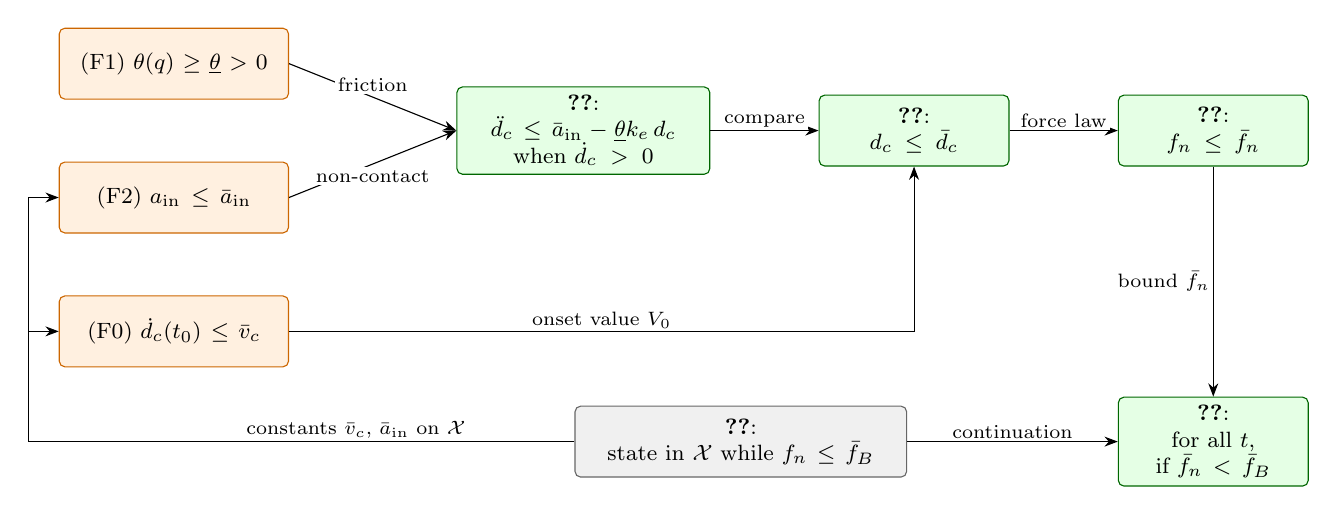
\begin{tikzpicture}[font=\footnotesize, >=Stealth,
  hyp/.style={draw=orange!80!black, fill=orange!12, rounded corners=2pt, align=center, inner sep=3pt, text width=27mm, minimum height=9mm},
  res/.style={draw=green!40!black, fill=green!10, rounded corners=2pt, align=center, inner sep=3pt, text width=22mm, minimum height=9mm},
  ext/.style={draw=black!60, fill=black!6, rounded corners=2pt, align=center, inner sep=3pt, text width=40mm, minimum height=9mm},
  lab/.style={font=\scriptsize, fill=white, inner sep=1pt}]
\node[hyp] (f1) at (0,1.7) {(F1) $\theta(q)\ge\underline\theta>0$};
\node[hyp] (f2) at (0,0) {(F2) $a_{\mathrm{in}}\le\bar a_{\mathrm{in}}$};
\node[hyp] (f0) at (0,-1.7) {(F0) $\dot d_c(t_0)\le\bar v_c$};
\node[res, text width=30mm] (nd) at (5.2,0.85) {\Cref{fact:normal}:\\ $\ddot d_c\le\bar a_{\mathrm{in}}-\underline\theta k_e\,d_c$\\ when $\dot d_c>0$};
\node[res] (lem) at (9.4,0.85) {\Cref{lem:scalar}:\\ $d_c\le\bar d_c$};
\node[res] (thm) at (13.2,0.85) {\Cref{thm:force}:\\ $f_n\le\bar f_n$};
\node[ext] (jb) at (7.2,-3.1) {\Cref{thm:r1}:\\ state in $\mathcal X$ while $f_n\le\bar f_B$};
\node[res] (cl) at (13.2,-3.1) {\Cref{thm:closure}:\\ for all $t$,\\ if $\bar f_n<\bar f_B$};
\draw[->] (f1.east) -- node[lab, above, pos=0.5, yshift=1pt] {friction} (nd.west);
\draw[->] (f2.east) -- node[lab, below, pos=0.5, yshift=-1pt] {non-contact} (nd.west);
\draw[->] (nd) -- node[lab, above] {compare} (lem);
\draw[->] (f0.east) -| node[lab, pos=0.25, above] {onset value $V_0$} (lem.south);
\draw[->] (lem) -- node[lab, above] {force law} (thm);
\draw[->] (thm) -- node[lab, left] {bound $\bar f_n$} (cl);
\draw[->] (jb) -- node[lab, above] {continuation} (cl);
\draw[->] (jb.west) -| node[lab, pos=0.2, above] {constants $\bar v_c$, $\bar a_{\mathrm{in}}$ on $\mathcal X$} (-1.85,-1.7) -- (f0.west);
\draw[->] (-1.85,-1.7) |- (f2.west);
\end{tikzpicture}
\caption{Dependency chain of the contact force bound}
\label{fig:forcechain}
\end{figure}

\begin{definition}[Compliant surface]
\label{def:surface}
In the setting of \Cref{def:robot}, let $x_c(q)\in\R^{n_c}$ be the contact point, $J_c=\partial x_c/\partial q$. A \textbf{\emph{compliant surface}} is given by a point $x_s\in\R^{n_c}$, a unit normal $n\in\R^{n_c}$ and constants $k_e>0$, $\delta_e\ge0$, $\nu_e\ge0$.
\begin{itemize}
\item Depth: $d_c:=-n^\top(x_c-x_s)\in\R$, so that $\dot d_c=-n^\top v_c$; $d_c^+:=\max\{d_c,0\}$ and $\dot d_c^+:=\max\{\dot d_c,0\}$.
\item Force: $f_e=f_n\,n+f_t$ with $n^\top f_t=0$,
\[
f_n:=k_e\,d_c^+\,\max\{0,\ 1+\delta_e\,\dot d_c\},\qquad \|f_t\|\le\nu_ef_n .
\]
\item Class: $\mathcal S(\bar k_e,\bar\delta_e,\bar\nu_e)$ is the set of compliant surfaces with $k_e\le\bar k_e$, $\delta_e\le\bar\delta_e$, $\nu_e\le\bar\nu_e$; $x_s$, $k_e$, $\delta_e$, $\nu_e$ are unknown to the controller.
\item A \textbf{\emph{contact interval}} is an interval $[t_0,t_1]$ without events on which $d_c(t)\ge0$.
\end{itemize}
\end{definition}

\Cref{def:stageBplant}의 block 윗면은 $n=(0,1)$, $d_c=d_{\mathrm{top}}$인 compliant surface이다.

\begin{definition}[Two kinds of constraints]
\label{def:kinds}
Two kinds of requirements on a solution of \Cref{def:robot} are distinguished.
\begin{itemize}
\item A \textbf{\emph{keep-out constraint}} for a set $\mathcal K_o$ of states requires $(q,\dot q)(t)\notin\mathcal K_o$ $\ \forall t\ge0$.
\item A \textbf{\emph{contact-permitting constraint}} with the force limit $\bar f_c>0$ on a compliant surface requires
\[
\|f_e(t)\|\le\bar f_c\qquad\forall t\ge0 ,
\]
and places no requirement on $d_c$ or $v_c$.
\end{itemize}
\end{definition}

관절 상자 $q\in\mathcal C_q$는 keep-out constraint이고 \Cref{thm:r1}이 다룬다. 이 절은 contact-permitting constraint를 다룬다.

\begin{definition}[Quantities of the normal dynamics]
\label{def:normal}
For a compliant surface of $\mathcal S(\bar k_e,\bar\delta_e,\bar\nu_e)$:
\begin{itemize}
\item $\Upsilon(q):=J_c(q)M(q)^{-1}J_c(q)^\top\in\R^{n_c\times n_c}$, the inverse of the operational-space inertia where $J_c$ has full row rank;
\item $\theta(q):=n^\top\Upsilon(q)\,n-\bar\nu_e\,\|(I-nn^\top)\Upsilon(q)\,n\|\in\R$;
\item $a_{\mathrm{in}}(q,\dot q,\tau):=-n^\top\big(J_cM^{-1}(\tau-C\dot q-g-F_v\dot q+d)+\dot J_c\dot q\big)\in\R$, the inward acceleration of the contact point without the contact force.
\end{itemize}
\end{definition}

\begin{fact}[Normal dynamics]
\label{fact:normal}
On a contact interval, for almost every $t$,
\[
\ddot d_c=a_{\mathrm{in}}-n^\top\Upsilon f_e\ \le\ a_{\mathrm{in}}-\theta(q)\,f_n .
\]
\end{fact}

\begin{proof}
\[
\ddot d_c=-n^\top\big(J_c\ddot q+\dot J_c\dot q\big),\qquad \ddot q=M^{-1}\big(\tau-C\dot q-g-F_v\dot q+d+J_c^\top f_e\big)
\]
\[
\Longrightarrow\quad \ddot d_c=a_{\mathrm{in}}-f_n\,n^\top\Upsilon n-n^\top\Upsilon f_t .
\]
$n^\top f_t=0$이므로 $n^\top\Upsilon f_t=\big((I-nn^\top)\Upsilon n\big)^\top f_t$이다.
\[
-n^\top\Upsilon f_t\le\|(I-nn^\top)\Upsilon n\|\,\|f_t\|\le\bar\nu_e\,\|(I-nn^\top)\Upsilon n\|\,f_n .
\]
\end{proof}

\begin{lemma}[Scalar comparison]
\label{lem:scalar}
Let $\varkappa>0$, $b\in\R$, and let $y:[t_0,t_1]\to[0,\infty)$ be $C^1$ with $\dot y$ absolutely continuous and
\[
\ddot y(t)\le b-\varkappa\,y(t)\qquad\text{for almost every $t$ with }\dot y(t)>0 .
\]
With $\dot y^+:=\max\{\dot y,0\}$, $V_y:=\tfrac12(\dot y^+)^2+\tfrac12\varkappa\,y^2-b\,y$ and $V_0:=\max\{V_y(t_0),0\}$, for all $t\in[t_0,t_1]$:
\begin{enumerate}[label=(\alph*)]
\item $V_y(t)\le V_0$;
\item $y(t)\le\dfrac{b+\sqrt{b^2+2\varkappa V_0}}{\varkappa}$.
\end{enumerate}
\end{lemma}

\begin{proof}
\textbf{Step 1 (rate of $V_y$).} $V_y$는 절대 연속이고, 거의 모든 $t$에서 다음이 성립한다.
\[
\dot V_y=\begin{cases}\dot y\,\big(\ddot y+\varkappa\,y-b\big)\le0, & \dot y>0,\\[2pt] \big(\varkappa\,y-b\big)\dot y, & \dot y\le0.\end{cases}
\]
\textbf{Step 2 (the second case where $V_y>0$).} $\dot y\le0$이고 $V_y>0$이면 $V_y=y\,(\tfrac12\varkappa\,y-b)>0$이다.
\[
y>0,\quad \tfrac12\varkappa\,y>b\quad\Longrightarrow\quad \varkappa\,y-b>0\quad\Longrightarrow\quad \dot V_y\le0 .
\]
\textbf{Step 3 (a).} $V_y(t_2)>V_0$인 $t_2$가 있다고 하고 $s:=\sup\{t\le t_2:\ V_y(t)\le V_0\}$로 둔다. $V_y(s)=V_0$이고 $(s,t_2]$에서 $V_y>V_0\ge0$이므로, Step 1과 Step 2에 의해 그 구간에서 거의 어디서나 $\dot V_y\le0$이다.
\[
V_y(t_2)=V_y(s)+\int_s^{t_2}\dot V_y\,dt\le V_0 .
\]
이는 $V_y(t_2)>V_0$과 모순이다.

\textbf{Step 4 (b).}
\[
\tfrac12\varkappa\,y^2-b\,y\le V_y\le V_0\quad\Longrightarrow\quad y\le\frac{b+\sqrt{b^2+2\varkappa V_0}}{\varkappa} .
\]
\end{proof}

\begin{theorem}[Contact force bound]
\label{thm:force}
Consider a solution of \Cref{def:robot} on a contact interval $[t_0,t_1]$ with a compliant surface of $\mathcal S(\bar k_e,\bar\delta_e,\bar\nu_e)$, and let $\underline\theta>0$ and $\bar a_{\mathrm{in}}\in\R$ satisfy
\begin{itemize}
\item[\textbf{(F1)}] $\theta(q(t))\ge\underline\theta$ $\ \forall t\in[t_0,t_1]$;
\item[\textbf{(F2)}] $a_{\mathrm{in}}(t)\le\bar a_{\mathrm{in}}$ for almost every $t\in[t_0,t_1]$ with $\dot d_c(t)>0$.
\end{itemize}
Let $\varkappa:=\underline\theta\,k_e$, $V_0:=\max\{\tfrac12\dot d_c^+(t_0)^2+\tfrac12\varkappa\,d_c(t_0)^2-\bar a_{\mathrm{in}}\,d_c(t_0),\,0\}$ and $F_{\mathrm{in}}:=\bar a_{\mathrm{in}}/\underline\theta$. Then for all $t\in[t_0,t_1]$:
\begin{enumerate}[label=(\alph*)]
\item $d_c(t)\le\bar d_c:=\dfrac{\bar a_{\mathrm{in}}+\sqrt{\bar a_{\mathrm{in}}^2+2\varkappa V_0}}{\varkappa}$;
\item $f_n(t)\le k_e\,\bar d_c\,\big(1+\delta_e\,\dot d_c^+(t)\big)$, where $k_e\,\bar d_c=F_{\mathrm{in}}+\sqrt{F_{\mathrm{in}}^2+2k_eV_0/\underline\theta}$;
\item if $d_c(t_0)=0$ and $\|v_c\|\le\bar v_c$ on $[t_0,t_1]$, then
\[
f_n(t)\le(1+\delta_e\,\bar v_c)\Big(F_{\mathrm{in}}+\sqrt{F_{\mathrm{in}}^2+k_e\,\bar v_c^2/\underline\theta}\Big),\qquad \|f_e(t)\|\le\sqrt{1+\nu_e^2}\,f_n(t) .
\]
\end{enumerate}
Scope: one solution and one contact interval; no assumption on the brain, the hand or the weights beyond (F1) and (F2); regional in the configuration through (F1).
\end{theorem}

\begin{proof}
$\dot d_c>0$인 시각에는 $f_n=k_e\,d_c\,(1+\delta_e\dot d_c)\ge k_e\,d_c$이다. \Cref{fact:normal}, (F1), (F2)를 쓴다.
\[
\ddot d_c\le a_{\mathrm{in}}-\theta(q)\,f_n\le\bar a_{\mathrm{in}}-\underline\theta\,k_e\,d_c\qquad\text{for almost every $t$ with }\dot d_c(t)>0 .
\]
\Cref{lem:scalar}를 $y=d_c$, $b=\bar a_{\mathrm{in}}$, $\varkappa=\underline\theta k_e$로 쓰면 (a)이다. (b)는 힘의 정의와 (a)이다.
\[
f_n=k_e\,d_c\,\max\{0,1+\delta_e\dot d_c\}\le k_e\,\bar d_c\,(1+\delta_e\,\dot d_c^+) .
\]
(c)에서는 $d_c(t_0)=0$이고 $\dot d_c^+\le\|v_c\|\le\bar v_c$이다.
\[
V_0=\tfrac12\dot d_c^+(t_0)^2\le\tfrac12\bar v_c^2\quad\Longrightarrow\quad k_e\,\bar d_c\le F_{\mathrm{in}}+\sqrt{F_{\mathrm{in}}^2+k_e\,\bar v_c^2/\underline\theta} .
\]
\[
\|f_e\|^2=f_n^2+\|f_t\|^2\le(1+\nu_e^2)\,f_n^2 .
\]
\end{proof}

\textbf{해석 (상한의 두 항과 조건의 뜻).} $F_{\mathrm{in}}$은 접촉 중 안쪽으로 미는 구동이 정적으로 낼 수 있는 힘이고, $\sqrt{k_e\bar v_c^2/\underline\theta}$는 충돌의 몫이다. $1/\underline\theta$는 접촉점이 법선 방향으로 보이는 가장 큰 유효 질량에 해당한다. 마찰이 없으면 $\theta=n^\top\Upsilon n$이고, Cauchy--Schwarz 부등식에서 충돌의 몫은 접촉 시작 순간의 운동 에너지로 제한된다.
\[
\frac{\dot d_c^2}{n^\top\Upsilon n}=\frac{(n^\top J_c\dot q)^2}{n^\top J_cM^{-1}J_c^\top n}\le\dot q^\top M\dot q .
\]
자유도가 하나이고 구동이 일정하며 $\delta_e=0$이면 깊이는 (a)의 상한 $\bar d_c$에 도달한다. 상한에 들어가는 양은 $\bar v_c$, $\bar a_{\mathrm{in}}$, $\underline\theta$, $k_e$, $\delta_e$뿐이고, 표면의 위치 $x_s$와 표면까지의 거리는 들어가지 않는다. 그래서 이 보장은 표면 가까이에서 운동을 따로 제한하지 않으며, 그 대가는 $\bar v_c$가 모든 곳에서 같은 한도라는 것이다. (F1)이 깨지는 자세에서는 마찰력이 관성의 결합을 거쳐 접촉점을 안쪽으로 가속하는 몫이 법선 힘이 밀어내는 몫보다 클 수 있다. 강체 접촉에서 Painlev\'e paradox로 알려진 영역이며(Champneys와 V\'arkonyi, 2016), 이 정리는 그 영역을 다루지 않는다.

\begin{corollary}[Speed limit and delayed relief]
\label{cor:reaction}
In the setting of \Cref{thm:force} with $d_c(t_0)=0$, let $\bar v\ge0$, $t_d\ge0$ and $a_r\ge0$ satisfy (F1) and
\begin{itemize}
\item[\textbf{(F0)}] $\dot d_c(t)\le\bar v$ $\ \forall t\in[t_0,t_1]$;
\item[\textbf{(F2$'$)}] $a_{\mathrm{in}}(t)\le-a_r$ for almost every $t\in[t_0+t_d,t_1]$ with $\dot d_c(t)>0$.
\end{itemize}
With $\varkappa:=\underline\theta\,k_e$ and $V_d:=\tfrac12\bar v^2+\tfrac12\varkappa\,(\bar vt_d)^2+a_r\,\bar vt_d$, for all $t\in[t_0,t_1]$:
\begin{enumerate}[label=(\alph*)]
\item $d_c(t)\le\bar d_r:=\dfrac{-a_r+\sqrt{a_r^2+2\varkappa V_d}}{\varkappa}$;
\item $f_n(t)\le k_e\,\bar d_r\,(1+\delta_e\,\bar v)$.
\end{enumerate}
\end{corollary}

\begin{proof}
\textbf{Step 1 (before the relief).} $t\le t_0+t_d$이면 (F0)에서 다음이 성립한다.
\[
d_c(t)=\int_{t_0}^t\dot d_c\,ds\le\bar v\,t_d .
\]
\textbf{Step 2 (after the relief).} \Cref{thm:force}의 증명과 같이 \Cref{fact:normal}, (F1), (F2$'$)에서 $[t_0+t_d,t_1]$의 $\dot d_c>0$인 거의 모든 시각에 $\ddot d_c\le-a_r-\varkappa\,d_c$이므로, \Cref{lem:scalar}를 $b=-a_r$로 쓴다. 이때 $V_y=\tfrac12(\dot d_c^+)^2+\tfrac12\varkappa\,d_c^2+a_rd_c$는 $d_c\ge0$과 $\dot d_c^+$에 대해 증가하므로 Step 1과 (F0)에서 $V_y(t_0+t_d)\le V_d$이다.
\[
\tfrac12\varkappa\,d_c^2+a_r\,d_c\le V_d\quad\Longrightarrow\quad d_c\le\bar d_r .
\]
\textbf{Step 3 (both parts).} $x=\bar vt_d$는 $\tfrac12\varkappa x^2+a_rx\le V_d$를 만족하므로 $\bar vt_d\le\bar d_r$이고, (a)가 전체 구간에서 성립한다. (b)는 \Cref{thm:force}(b)의 논증과 (F0)이다.
\end{proof}

\textbf{해석 (구동의 상한을 누가 정하는가).} \Cref{thm:force}의 $\bar a_{\mathrm{in}}$을 구조가 정해 주지 않으면 입력 상자 전체가 그 값이 되고, $F_{\mathrm{in}}$은 actuator가 낼 수 있는 가장 큰 힘이 된다. 접촉을 감지한 뒤 학습되지 않는 요소가 밀어내는 방향의 torque를 더하면, 감지 지연 $t_d$ 뒤부터 구동의 부호가 바뀐다((F2$'$)). 지연 동안의 침투는 속도 한도 (F0)이 제한한다. 충돌을 감지하고 반응하는 구성은 로봇 충돌 처리의 표준이다(Haddadin 등, 2017). \Cref{def:guard}의 guard는 목표와 강성의 전진을 멈출 뿐 밀어내지 않으므로 (F2$'$)를 주지 않는다.

\begin{proposition}[Energy form for every friction coefficient]
\label{prop:energyforce}
Consider the tank of \Cref{def:fulltank}, $E_{\mathrm{rob}}$ of \Cref{thm:fulltank} and a compliant surface with any $\nu_e\ge0$ whose friction is dissipative, $v_c^\top f_t\le0$. On every interval $[t_0,t]$ without events,
\[
\tfrac12k_e\,d_c^+(t)^2\ \le\ \Delta_E(t_0,t):=\tfrac12k_e\,d_c^+(t_0)^2+\big(E_{\mathrm{rob}}(t_0)-E_{\mathrm{rob}}(t)\big)+\big(T(t_0)-T(t)\big),
\]
\[
f_n(t)\ \le\ \big(1+\delta_e\,\dot d_c^+(t)\big)\sqrt{2k_e\,\Delta_E(t_0,t)} .
\]
\end{proposition}

\begin{proof}
$S_e:=\tfrac12k_e(d_c^+)^2$로 둔다. $1+\delta_e\dot d_c\ge0$이면 $f_n\dot d_c=k_ed_c^+\dot d_c+k_ed_c^+\delta_e\dot d_c^2\ge k_ed_c^+\dot d_c$이고, 그렇지 않으면 $f_n=0$, $\dot d_c<0$이다.
\[
\dot S_e=k_e\,d_c^+\dot d_c\le f_n\,\dot d_c,\qquad v_c^\top f_e=-f_n\,\dot d_c+v_c^\top f_t\le-\dot S_e .
\]
\Cref{thm:fulltank}(a)와 $F_v\succeq0$을 쓰고 적분한다.
\[
\frac{d}{dt}\big(E_{\mathrm{rob}}+T+S_e\big)\le-\dot q^\top F_v\dot q\le0 .
\]
힘은 정의에서 $f_n\le k_e\,d_c^+\,(1+\delta_e\dot d_c^+)=(1+\delta_e\dot d_c^+)\sqrt{2k_eS_e}$이다.
\end{proof}

\textbf{해석 (마찰과 무관한 형태와 그 한계).} 이 부등식은 (F1)을 쓰지 않는다. 표면에 쌓이는 에너지는 로봇의 역학적 에너지가 줄어든 양과 tank가 지불한 양의 합을 넘지 못한다. $\theta(q)\le0$인 자세에서 마찰이 침투를 키우더라도 그 에너지의 출처는 이 둘뿐이다. \Cref{thm:force}와의 차이는 둘이다. 충돌의 몫에 법선 방향 유효 질량의 운동 에너지가 아니라 팔 전체의 운동 에너지가 들어가고, 우변이 접촉 시작부터의 누적량이어서 오래 누르거나 미끄러지는 접촉에서는 class 수준의 상수가 되지 않는다. Class 수준의 상한으로 쓰려면 접촉 중 tank가 지불하는 양과 위치 에너지가 줄어드는 양을 구조가 제한해야 하며, 그 요소는 정해지지 않았다.

\begin{theorem}[Closure of the joint box and the force bound]
\label{thm:closure}
With the gauge and the coordinates of \Cref{def:cons3} and \Cref{thm:r1}, let
\[
\mathcal X:=\{(q,\dot q):\ \rho(w)<1,\ \rho(w_q)<1\},
\]
\[
\mathcal F(\bar f_B):=\{f_n\,n+f_t:\ 0\le f_n\le\bar f_B,\ n^\top f_t=0,\ \|f_t\|\le\bar\nu_ef_n\},
\]
and assume, for every hand and brain weight, every proposal, every plant of the class and every solution with $(q,\dot q)(0)\in\mathcal X$ and every $t_1>0$:
\begin{itemize}
\item[\textbf{(J)}] $f_e(s)\in\mathcal F(\bar f_B)$ $\ \forall s\in[0,t_1)$ $\ \Longrightarrow\ $ $(q,\dot q)(t)\in\mathcal X$ $\ \forall t\in[0,t_1)$.
\end{itemize}
Let $\mathcal Q_c$ contain every configuration at which the contact point touches a surface of $\mathcal S(\bar k_e,\bar\delta_e,\bar\nu_e)$, let $\mathcal X_c:=\{(q,\dot q)\in\overline{\mathcal X}:\ q\in\mathcal Q_c\}$, and define, with suprema and infimum also over the plants of the class,
\[
\bar v_c:=\sup_{\mathcal X_c}\|J_c\dot q\|,\qquad \bar a_{\mathrm{in}}:=\max\Big\{0,\ \sup_{\mathcal X_c,\ \tau\in\U}a_{\mathrm{in}}\Big\},\qquad \underline\theta:=\inf_{\mathcal Q_c}\theta(q),
\]
\[
\bar f_n:=(1+\bar\delta_e\,\bar v_c)\Big(\frac{\bar a_{\mathrm{in}}}{\underline\theta}+\sqrt{\frac{\bar a_{\mathrm{in}}^2}{\underline\theta^2}+\frac{\bar k_e\,\bar v_c^2}{\underline\theta}}\Big) .
\]
If $\underline\theta>0$ and $\bar f_n<\bar f_B$, then for every hand and brain weight, every proposal, every plant of the class, every surface of $\mathcal S(\bar k_e,\bar\delta_e,\bar\nu_e)$ and every solution with $(q,\dot q)(0)\in\mathcal X$, $d_c(0)\le0$ and events only at times with $d_c<0$:
\begin{enumerate}[label=(\alph*)]
\item $f_n(t)\le\bar f_n$ $\ \forall t\ge0$;
\item $(q,\dot q)(t)\in\mathcal X$ $\ \forall t\ge0$, in particular $q(t)\in\mathcal C_q$.
\end{enumerate}
Scope: global in the weights and proposals; conditional on (J), $\underline\theta>0$ and $\bar f_n<\bar f_B$; one flat surface.
\end{theorem}

\begin{proof}
\textbf{Step 1 (first violation time).} $f_n$은 시간에 대해 연속이고 $f_n(0)=0$이다.
\[
t_f:=\sup\{t_1\ge0:\ f_n(t)\le\bar f_B\ \ \forall t\in[0,t_1]\}>0 .
\]
$t_f<\infty$라고 가정한다. $[0,t_f)$에서 $f_e\in\mathcal F(\bar f_B)$이므로 (J)와 연속성에서 다음이 성립한다.
\[
(q,\dot q)(t)\in\overline{\mathcal X}\qquad\forall t\in[0,t_f] .
\]
\textbf{Step 2 (force on $[0,t_f]$).} $d_c(t)>0$인 $t\le t_f$에 대해 $t_0:=\sup\{s\le t:\ d_c(s)\le0\}$로 두면 $[t_0,t]$는 $d_c(t_0)=0$인 contact interval이다. 그 위에서 $(q,\dot q)\in\mathcal X_c$이고 $\tau\in\U$이므로 (F1), (F2)가 $\underline\theta$, $\bar a_{\mathrm{in}}$으로 성립하고 $\|v_c\|\le\bar v_c$이다. \Cref{thm:force}(c)를 쓴다.
\[
f_n(t)\le(1+\delta_e\,\bar v_c)\Big(\frac{\bar a_{\mathrm{in}}}{\underline\theta}+\sqrt{\frac{\bar a_{\mathrm{in}}^2}{\underline\theta^2}+\frac{k_e\,\bar v_c^2}{\underline\theta}}\Big)\le\bar f_n<\bar f_B\qquad\forall t\in[0,t_f] .
\]
\textbf{Step 3 (contradiction).} $f_n$의 연속성에서 $\exists\,\epsilon>0$: $[t_f,t_f+\epsilon]$에서 $f_n\le\bar f_B$이다. 이는 $t_f$의 정의와 모순이므로 $t_f=\infty$이다. Step 2가 모든 $t$에서 성립하여 (a)이고, (J)에서 (b)이다.
\end{proof}

\textbf{해석 (서로를 가정하는 두 결과).} \Cref{thm:r1}은 접촉력이 유계라는 조건 (B2)를 가정으로 두었고, 그 한도를 구조가 보장한다는 결과는 없었다. \Cref{thm:force}는 반대로 상태가 유계인 집합에 머문다는 것을 필요로 한다. 순환을 끊는 것은 미리 정한 상수이다. 집합 $\mathcal X$와 입력 상자에서 계산한 상수로 $\bar f_n$을 정해 두고, 그 값이 $\bar f_B$보다 작으면 힘이 $\bar f_B$에 처음 닿는 시각이 존재할 수 없다. 조건 (J)는 \Cref{thm:r1}에서 (B2)와 (B3)의 힘의 범위를 $\mathcal F(\bar f_B)$로 둔 것이다. \Cref{thm:r1}의 증명은 힘의 범위가 compact라는 것과 gauge가 처음 1에 닿는 시각 이전의 힘만 쓰므로, (B1), $\mathcal F(\bar f_B)$ 위의 (B3), (B4)에서 (J)가 나온다. $\bar f_n<\bar f_B$가 성립하면 (B2)는 가정이 아니라 결론이 된다. 속도 한도와 지연된 반응이 구조에 있으면 Step 2의 상한을 \Cref{cor:reaction}의 값으로 바꾸어 같은 논증을 쓴다. Stage B의 상수와 이 조건의 성립 여부는 \Cref{sec:contactnum}에 있다.

\subsection{뇌와 에너지 장부}

\begin{definition}[Brain]
\label{def:brain}
The \textbf{\emph{brain}} is a network $\mu_W:o_k\mapsto a_k$ evaluated every $T_h$, with observation $o_k:=(q,\dot q,\hat\tau_{\mathrm{ext}},\chi,\ell_k)$, which contains neither the realized goal $q_d$ nor the realized stiffness $K$, and action
\[
a_k:=(q_d^p,\ K^p,\ \psi_k,\ \beta)\in\mathcal C_q\times[k_{\mathrm{lo}},k_{\mathrm{hi}}]^m\times\Psi\times\mathcal B,
\]
where $\chi$ is the task context, $\ell_k$ the ledger of \Cref{def:ledger}, $\psi_k$ the gripper command of \Cref{def:stageBplant} with $\Psi:=\{0,1\}$ for a plant with a gripper and $\Psi:=\{0\}$ otherwise, and $\mathcal B$ a compact set.
\end{definition}

\textbf{결정 (개정 16, 2026년 11월 15일).} Stage B의 뇌는 goal을 task 공간의 변위로 낸다. Network의 출력 $u$에서
\[
q_d^p:=\Pi_{\mathcal C_q}\big(q+J_{\mathrm{nom}}(q)^{+}\Delta p+n\,v_N(q)\big),\qquad \Delta p=0.3\tanh(u_{1:2})\ \mathrm{m},\qquad n=0.3\tanh(u_3)\ \mathrm{rad}
\]
이다. $J_{\mathrm{nom}}$은 공칭 길이의 Jacobian(class 수준의 기구학), $J_{\mathrm{nom}}^{+}$은 감쇠한 pseudo-inverse, $v_N$은 그 kernel의 단위 방향, $q$는 측정 자세이다. $q_d^p\in\mathcal C_q$이므로 정의와 그 위의 보장은 바뀌지 않는다. 같은 조건의 결정 실험에서 옮기기의 오차가 관절 공간의 절대 자세의 절반 이하였다(\Cref{sec:l2pt}).

\begin{definition}[Ledger]
\label{def:ledger}
On each decision interval $[t_k,t_{k+1})$ the \textbf{\emph{ledger}} is
\[
\ell_k:=\big(T(t_k),\ \bar\lambda_k,\ \hat u_{\mathrm{load}}(t_k)\big)\in\R\times(0,1]\times\R^m,
\]
with the tank level $T$, the interval mean $\bar\lambda_k$ of the saturation factor $\lambda:=1/\max\{1,\max_i|v_i|/\bar u_i\}$ of $v:=\alpha\tau_h+\tau_b$, and the \textbf{\emph{learned load}}
\[
\hat u_{\mathrm{load}}:=u_{\mathrm{ad}}-G_W(q)^\top\bar a_W=G_W(q)^\top\Gamma z_a ,
\]
the part of the compensation the memory has learned in the current episode. Each entry depends on the applied torque or on the hand's internal state.
\end{definition}

\textbf{해석 (지표의 의미).} $T$는 남은 에너지 예산, $\bar\lambda$는 손이 입력 한계에 얼마나 가까이 쓰이고 있는지, $\hat u_{\mathrm{load}}$는 손이 이번 episode에 들고 있다고 판단한 부하이다. 손이 부하를 보정하고 나면 spring의 처짐이 0으로 돌아가 부하의 흔적이 뇌의 관측에서 사라지므로, 뇌가 부하를 아는 길은 이 항목뿐이다. 뇌는 이 값을 의도 수준의 결정에 쓰고, 보상 자체는 손이 맡는다. Stage B에서는 누르기의 목표 힘을 물체 질량의 등급으로 고르는 데 쓴다(\Cref{def:stageBtask}(g)). 뇌가 이 값으로 목표를 옮겨 손의 몫을 가로채는지는 PRI로 잰다(\Cref{def:rvp}).

\textbf{결정 (2026년 11월 14일, 무엇을 장부에서 뺐나).} 장부에는 뇌가 다른 관측에서 계산할 수 없는 항목만 둔다. 그래서 다음을 뺐다. 제약 활동 $a$는 $q$와 $\dot q$의 함수이다. Spring 힘 $Ke_q$와 측정된 mismatch $\hat m$은 개정 12까지 뇌가 관측한 $q_d$와 $K$로 계산할 수 있어서 뺐다. 개정 13부터 뇌는 $q_d$와 $K$를 보지 않지만 둘을 다시 넣지 않는다. $Ke_q$는 실현 목표를 드러내고, $\hat m$도 gate가 열려 있고 제약층과 saturation이 작동하지 않으면 $s(Ke_q)+D_W\dot q-\hat\tau_{\mathrm{ext}}$이어서(\Cref{fact:mhat}) 마찬가지이며, 실현 목표를 아는 뇌는 적분 동작으로 손의 몫을 대신할 수 있기 때문이다(\Cref{fact:noint}). 정지 표시 $\zeta$는 측정된 속도의 이력이다. 주입 에너지와 gate 인자는 손의 torque에 달려 있지만 $T$에 의해 거의 정해지므로 단순화를 위해 뺐다. 감지된 접촉 torque $\hat\tau_{\mathrm{ext}}$는 장부가 아니라 뇌의 직접 관측이다. 개정 10까지의 장부는 부록이 아닌 이 문단에만 기록한다: $(T,E^{\mathrm{inj}},Ke_q,\hat\tau_{\mathrm{ext}},\hat m,\bar\zeta,\bar\alpha,\bar\lambda,\bar a)$.

\section{학습 framework}
\label{sec:learning}

\textbf{직관 (하나의 loop에서 서로를 보며 배운다).} 층을 따로 학습하면 각 층이 상대가 실제로 무엇을 요구하고 무엇을 할 수 있는지 모르게 되고, 하나의 return으로 모든 parameter를 학습하면 역할이 정해지지 않는다. 그래서 모든 층을 같은 rollout에서 함께 갱신하되, 각 층에는 자기 역할에 귀속되는 신호를 주고, 서로의 상태는 에너지 장부로 보게 한다.

\begin{definition}[Coupled learning]
\label{def:coupled}
The slow weights $W=(W_\mu,W_h)$ consist of the brain $W_\mu$ and the hand $W_h$, with the hand's damping network $D_W$ and memory parameters $(G_W,\bar a_W,\Gamma)$; the tank, gate, guard and constraint-layer constants are fixed. They are trained as follows.
\begin{itemize}
\item[\textbf{(L1)}] (Shared rollouts) Every update uses the same rollouts of the composed loop of \Cref{fig:arch3}; exploration perturbs the brain's action $a_k$ only.
\item[\textbf{(L2)}] (Role objectives) The brain maximizes
\[
J_\mu(W):=\mathbb E\Big[\sum_k\gamma^kr_k\Big],
\]
and the hand minimizes, with $u^\star$ available in simulation only,
\[
L_h(W):=\mathbb E\Big[\sum_k\int_{t_k}^{t_{k+1}}w(t)\,\|u_{\mathrm{ad}}-u^\star\|^2\,dt\Big]-c_r\,J_\mu(W),
\]
with the weight $w(t):=1-e^{-\lambda_s r(t)}\in[0,1]$, the rest time $r(t):=\int_{t_c(t)}^{t}\zeta(s)\,ds$ since the last change of the attached load, $t_c(t):=\sup\{s\le t:\ \xi(s^-)\ne\xi(s^+)\}$, and $r(t):=\infty$ if no change occurs before $t$.
\item[\textbf{(L3)}] (Observation coupling) The brain observes the ledger $\ell_k$; the brain's goal, stiffness and modulation enter the hand.
\item[\textbf{(L4)}] (Two time scales) The hand is updated with step sizes $\alpha_h$ and the brain with $\alpha_\mu$, $\ \alpha_\mu/\alpha_h\to0$.
\item[\textbf{(L5)}] (Guarantee-preserving parametrizations) Every slow weight ranges over a class for which \Cref{thm:fulltank} and the constraint guarantee hold for every value; slow weights change only between episodes.
\item[\textbf{(L6)}] (Deployable observations) Every entry of $o_k$ is computable from measured and internal signals; privileged quantities ($u^\star$, plant parameters, $f_e$) appear only in training losses.
\end{itemize}
\end{definition}

\textbf{해석 (결합이 일어나는 곳).} 결합은 세 곳에서 일어난다. 첫째, 손의 loss는 현재 뇌가 실제로 내는 요구의 분포 위에서 계산되므로, 손은 일반적인 reference가 아니라 이 뇌의 요구에 맞는 적응 방식을 배운다. 둘째, 뇌는 장부(tank 수준 $T$, saturation 비율 $\bar\lambda$, 손이 학습한 부하 $\hat u_{\mathrm{load}}$, \Cref{def:ledger})를 관측하므로, 예산이 부족할 때 천천히 다가가고 강성을 낮추는 행동과, 손이 추정한 부하로 질량 등급을 정하는 행동을 배울 수 있다. 셋째, tank가 두 층을 동역학으로 묶는다. 뇌가 많이 요구하면 예산이 줄어 실행이 늦어지고, 그 결과가 return으로 돌아온다. 최적의 접근 속도와 강성이 예산과 mismatch에 따라 달라지므로, 이 지표들은 v2의 보고와 달리 뇌의 결정을 바꾼다.

\textbf{해석 (역할의 귀속).} 기억과 feature는 mismatch로, 뇌는 task return으로 배우고, 둘은 같은 rollout과 상호 관측으로 서로의 상태를 안다. 단일 return에서 생기는 역할 혼동과 분리 학습에서 생기는 상호 무지를 함께 피하려는 설계이다. 두 시간 척도는 뇌가 자기 요구 분포에 거의 맞춰진 손을 보며 배우게 한다. 수렴 분석에는 두 시간 척도 확률 근사 이론을 도구로 쓸 수 있다.

\begin{lemma}[Rest-time floor of the mismatch]
\label{lem:restfloor}
Under \Cref{def:hand}, assume on an interval $[t_c,t]$ that $q$ and $u^\star$ are constant, $\zeta\equiv1$, $n=0$, $z_a\in\operatorname{int}\mathcal Z_0$ and $\operatorname{rank}G_W(q)=m$. Then
\[
\|u_{\mathrm{ad}}(t)-u^\star\|\ \ge\ e^{-\lambda_s(t-t_c)}\,\|u_{\mathrm{ad}}(t_c)-u^\star\|,
\]
with equality in the limit $\varepsilon\to0$.
\end{lemma}

\begin{proof}
$e:=u_{\mathrm{ad}}-u^\star$, $B:=G_W^\top\Gamma G_W\succ0$로 둔다. 정지와 $n=0$이면 \Cref{fact:mhat}에서
\[
\hat m=e .
\]
$A:=B(B+\varepsilon I)^{-1}$로 두고 갱신 법칙을 $u_{\mathrm{ad}}$에 넣는다.
\[
\dot e=G_W^\top\Gamma\,\dot z_a=-\lambda_s\,A\,e
\]
$A$는 대칭이고 고유값은 $\sigma_i/(\sigma_i+\varepsilon)\in(0,1)$이다($\sigma_i$는 $B$의 고유값).
\[
e(t)=e^{-\lambda_s(t-t_c)A}\,e(t_c)
\]
\[
\Longrightarrow\quad \|e(t)\|\ge e^{-\lambda_s(t-t_c)\lambda_{\max}(A)}\,\|e(t_c)\|\ge e^{-\lambda_s(t-t_c)}\,\|e(t_c)\|
\]
$\varepsilon\to0$이면 $A\to I$이므로 등호가 된다.
\end{proof}

\textbf{해석 (손이 책임지는 몫).} 짐이 바뀐 순간의 mismatch 가운데 정지 시간 $r$ 뒤에도 남는 몫은, feature와 prior가 무엇이든 적어도 $e^{-\lambda_s r}$이다(\Cref{lem:restfloor}). 그래서 가중치 $w=1-e^{-\lambda_s r}$은 기억이 그때까지 지울 수 있었던 몫만큼만 오차를 손에 묻는다. 뇌가 정지할 시간을 주지 않아 생긴 오차는, 보정되지 않은 짐으로 팔이 처지는 형태로 뇌의 task return에 남는다. 보정이 끝난 뒤의 오차, 즉 한 자세의 보정이 다른 자세로 옮겨 가는 정도는 손의 몫으로 남는다. 가중치가 없으면 손은 피할 수 없는 오차를 줄이려고 뇌의 현재 행동이 드는 평균 짐을 prior에 넣는다. 이는 물리 대신 과제 통계를 배우는 것이고, L2의 시험 실행에서 그대로 나타났다(\Cref{sec:l2a1}). Lemma는 자세가 고정된 정지를 가정한다. 느린 운동이 섞인 실제 정지에서 $w$는 이 lemma에서 고른 설계이다.

\textbf{학습 절차.}
\begin{enumerate}
\item Task와 plant parameter를 뽑고, 현재 $W$와 $a_k$의 탐색으로 합성된 loop를 rollout한다. $(o_k,a_k,r_k,\ell_k)$와 시뮬레이션의 $u^\star$를 기록한다.
\item 손의 step: 기록된 rollout 위에서 손의 동역학을 통과하는 gradient(또는 $L_h$의 critic)로 $W_h$를 $-\alpha_h\nabla L_h$만큼 갱신한다. Slow weight는 episode 경계에서만 바꾼다.
\item 뇌의 step: RL 방법으로 $J_\mu$에 대해 $W_\mu$를 갱신한다($\alpha_\mu\ll\alpha_h$).
\item 반복한다. (L5)에 의해 모든 반복에서 보장이 유지된다.
\end{enumerate}

\section{R8과 R9: 회계 방식을 바꾼 근거}
\label{sec:r8r9}

\textbf{직관 (무엇이 드러났나).} 정상 상태 정확도(R8)를 설계하려고 수치로 확인하는 과정에서, 손의 기억을 $\dot q$로만 구동하면 미지의 중력을 배우지 못한다는 것이 드러났다. 또 힘 sensor 없이는 정지 상태에서 mismatch와 접촉 힘이 구별되지 않는다. 이 절은 그 근거와 수치 확인을 담으며, 그 결과로 승인된 재설계가 \Cref{sec:arch}에 반영되었다.

\begin{proposition}[Velocity-driven adaptation has no memory]
\label{prop:memoryless}
Let $m=1$, $n_f=0$ and $\dot z_a=-G_W(q)\,\dot q$ with $G_W$ continuous. Then, with $\Phi(q):=\int_{q(0)}^{q}G_W(s)\,ds\in\R^{n_a}$,
\[
z_a(t)=z_a(0)-\Phi\big(q(t)\big)\qquad\forall t .
\]
Hence $\hat c$ and $u_{\mathrm{ad}}$ are functions of $q(t)$ alone, and a mismatch at a configuration $\bar q$ is the same whenever $q=\bar q$. For $m\ge2$ the same holds whenever each row of $G_W$ is a gradient field.
\end{proposition}

\begin{proof}
연쇄 법칙으로 우변을 미분한다.
\[
\frac{d}{dt}\Big(z_a(0)-\Phi\big(q(t)\big)\Big)=-G_W\big(q(t)\big)\,\dot q(t)=\dot z_a(t) .
\]
두 식은 $t=0$에서 같다.
\end{proof}

\begin{proposition}[Rest indistinguishability without force sensing]
\label{prop:indist}
At every rest state ($\dot q=\ddot q=0$) under \Cref{def:hand},
\[
Ke_q=\big(u_{\mathrm{ad}}-u^\star\big)+J_c^\top f_e .
\]
Hence, from $(q,\dot q)$ alone, a mismatch $\mu\in\R^m$ without contact and an exact representation with a contact torque $J_c^\top f_e=\mu$ give the same measurement at rest.
\end{proposition}

\begin{proof}
정지 상태에서 운동 방정식은 다음과 같다.
\[
0=\tau_h-g+d+J_c^\top f_e=u_{\mathrm{ad}}-Ke_q-u^\star+J_c^\top f_e .
\]
\end{proof}

\textbf{수치 확인 1 (tank가 최악의 경우를 지불하는 calibration).} 정지 중 $Ke_q$로 기억을 구동하고, 그 일률의 최악값 $\varepsilon\|Ke_q\|(\|u_{\mathrm{ad}}\|+\bar u^\star)$을 tank가 지불하게 했다($\bar u^\star=18$). 지불이 tank를 즉시 $T_{\min}$(최솟값 0.500)까지 비웠고, 누르기 직전의 mismatch는 4.800--10.218 Nm로 calibration이 없을 때(5.563--10.224 Nm)와 거의 같았다. 벽에 닿은 경우는 0/16였다. Class 상한으로 지불하는 방식은 너무 보수적이다.

\textbf{수치 확인 2 (full-power tank와 뇌가 켜는 오차 구동 기억).} 뇌가 벽 앞의 자유 공간에서 정지한 1.5초 동안 기억을 $\dot q+\lambda_se_q$($\lambda_s=10$)로 구동하게 하고, 그 뒤 목표를 벽 뒤에 두어 눌렀다. 항등식 오차는 최대 $6.5\times10^{-11}$였다. 누르기 직전의 mismatch는 0.579--0.865 Nm로, calibration이 없을 때(5.902--11.454 Nm)의 약 10분의 1이었다. 벽에 닿은 경우는 calibration이 있을 때 3/4, 없을 때 0/4였고, 닿은 경우의 목표 접촉 torque(3 Nm) 오차는 1.091--1.150 Nm였다. 접촉 중에도 오차 구동 기억을 켜 두면 접촉 torque가 12.314--12.449 Nm로 목표의 4배를 넘었는데(3개 경우), tank는 최소 4.777로 고갈되지 않았다. 단단한 벽에서 큰 힘은 작은 에너지로 만들어지므로, 에너지 장부는 힘을 제한하지 못한다.

\textbf{수치 확인 3 (감지 기반 동결).} 수치 확인 2의 잘못된 사용(접촉 중 calibration 요청)에서, 감지된 접촉 torque가 0.5 Nm를 넘는 동안 calibration을 0으로 만들었다(감지 잡음 표준편차 0.05 Nm). 정상 상태 접촉 torque가 0.605--4.150 Nm로 줄었다(동결이 없을 때 12.314--12.449 Nm). 충돌 순간의 최대 접촉 torque는 최대 11.04 Nm로, 올바른 사용에서도 최대 7.02 Nm였다. 충돌 순간의 힘은 접근 속도와 감쇠가 정하므로 새 요구 사항 (R17)로 둔다.

\textbf{반영된 재설계.} (a) Passivity는 full-power tank로 얻는다(\Cref{sec:tank3}). (b) 기억은 정지 상태에서 측정된 mismatch로 갱신된다(\Cref{def:hand}; M1과 M2 점검의 결과로 개정). (c) 접촉 힘은 guard와 정적 상한으로 다룬다(\Cref{def:guard,prop:static}). (d) (R9)의 진행 보장은 task energy, 즉 과제를 passive하게 끝내는 데 필요한 최소 tank 에너지(Zanella 등)로 표현하며, 예산에는 중력에 대한 일이 포함된다. 이전 회계 방식(요구의 gating과 debt)의 정의와 결과는 부록에 남긴다.

\section{역할 학습과 검증}
\label{sec:roles}

\textbf{직관 (구조가 복잡할수록 역할을 따로 확인해야 한다).} M2에서 뇌와 손은 spring 한도와 치우친 기억으로 과제를 푸는 해법을 배웠고, 그동안 보장은 한 번도 깨지지 않았다(\Cref{sec:m2audit}). 보장은 역할의 올바름을 대신하지 못하므로, 역할이 의도대로 학습되게 하는 장치와 그것을 측정하는 평가가 따로 필요하다.

\textbf{학습 쪽 장치.}
\begin{itemize}
\item[\textbf{(T1)}] 역할별 목적: 기억은 mismatch, 뇌는 task return(\Cref{def:coupled}의 (L2)).
\item[\textbf{(T2)}] 학습 중에만 쓰는 특권 신호: $u^\star$, 접촉 여부, payload. 역할 학습의 목표로만 쓰고 관측에는 넣지 않는다.
\item[\textbf{(T3)}] Gradient 경로 분리: 손의 손실은 뇌를 갱신하지 않고, 뇌의 return은 손에 작은 가중치 $c_r$로만 들어간다.
\item[\textbf{(T4)}] 정보 구조: 뇌는 특권 정보(실제 payload, $u^\star$, plant parameter)를 보지 못하고, 부하에 관해서는 손의 추정치 $\hat u_{\mathrm{load}}$만 본다. 뇌가 그 값으로 목표를 옮겨 손의 몫을 가로채는지는 PRI로 잰다.
\item[\textbf{(T5)}] 단계적 과제: 접촉 없는 과제에서 시작해 접촉 과제로 넘어가되, 모든 단계에서 같은 rollout으로 함께 학습한다.
\item[\textbf{(T6)}] 학습 중 역할 감시: 아래 (V3)의 지표를 학습 중에 추적하고, 역할이 흐트러지면 경보를 낸다.
\end{itemize}

\begin{definition}[Role verification protocol]
\label{def:rvp}
Every evaluation of a trained system reports, in simulation:
\begin{itemize}
\item[\textbf{(V1)}] (Certificate audit) the residual of \Cref{thm:fulltank} per episode, constraint violations, $\min T$ and tank depletion events;
\item[\textbf{(V2)}] (Counterfactual ablation) for each module $\mathsf m$ in \{memory, ledger observation, intent channel\}, $\ \Delta_{\mathsf m}J:=J(\text{full})-J(\text{full retrained without }\mathsf m)$, and the same difference with $\mathsf m$ neutralized at test time (frozen memory, the ledger held at its training mean, or a constant intent);
\item[\textbf{(V3)}] (Role fidelity)
\begin{itemize}
\item mismatch fidelity $\ \bar e_{\mathrm{mis}}:=$ mean of $\|u_{\mathrm{ad}}-u^\star\|$ over free-space rest segments;
\item payload response index $\ \mathrm{PRI}:=\|\Delta q_d^p\|\big/\|K^{-1}\Delta u^\star\|$ after a payload change during a hold, with $\Delta q_d^p$ the change of the brain's goal and $\Delta u^\star$ the change of the required compensation; $\mathrm{PRI}\approx0$ when the memory absorbs the change and $\mathrm{PRI}\approx1$ when the brain does;
\item out-of-distribution retention: the ratio of task errors under payloads and contact stiffnesses outside the training range to those inside, with slow weights frozen;
\item ledger reliance: the fraction of observation perturbations $\delta T<0$ for which the brain lowers the requested stiffness or the goal step;
\end{itemize}
\item[\textbf{(V4)}] (Stress) contact stiffness beyond the training range, a payload change within an episode, a sweep of the budget $T(0)$, and link masses and lengths changed beyond the training range with slow weights frozen;
\item[\textbf{(V5)}] (Learning diagnostics) the role losses and the (V3) metrics along training.
\end{itemize}
Acceptance thresholds for (V1)--(V3) are fixed in the pre-registration of \Cref{sec:eval}.
\end{definition}

\textbf{해석 (무엇을 잡아내나).} (V1)은 구현이 보장을 실제로 지키는지, (V2)는 각 모듈이 성능에 기여하는지, (V3)는 그 기여가 의도한 역할을 통해서인지를 본다. 예를 들어 잡기 직후의 PRI가 1에 가까우면 뇌가 목표를 옮겨 부하를 보상하고 있다는 뜻이고, 분포 밖 무게에서 오차가 크게 늘면 그 분업이 학습 분포에만 맞춰졌다는 뜻이다.

\section{구현, 학습, 검증 계획}
\label{sec:plan}

\textbf{직관 (구조적 특징이 검증을 가능하게 한다).} Torque sensing과 full-power tank는 보장을 주는 동시에, 그 보장과 역할을 로봇 위에서 측정할 수 있게 만든다. Tank의 장부는 측정된 $\dot q$와 가한 $\tau$만으로 정확히 계산되고, 감지된 접촉 torque로 환경에 넘긴 에너지와 정지 상태의 mismatch를 직접 잴 수 있다. 계획은 이 측정 가능성을 구현, 학습, 검증의 각 단계에 넣는다.

\subsection{구현}

\begin{itemize}
\item \textbf{시간 구조.} 뇌는 $T_h=50$ ms마다, 손, tank, guard, 제약층은 $T_s=2$ ms마다 계산하고(최종 평가는 1 ms에서도 반복), torque는 그 사이에 일정하게 유지한다. Plant는 $T_s$ 안에서 4차 Runge--Kutta로 네 번 적분한다(\Cref{sec:envcheck}).
\item \textbf{이산 tank.} Torque가 한 주기 동안 일정하면 그 주기에 tank에서 빠지는 에너지는 정확히 다음과 같다(Zanella 등의 energy sampling).
\[
T_{k+1}=T_k-\tau_k^\top\big(q_{k+1}-q_k\big)
\]
Gate는 $T_k$로 $\alpha_k$를 정하므로 한 주기 지연이 있고, 그 주기 안의 초과는 $\|\tau_k\|\,\|q_{k+1}-q_k\|$ 이하이다. $T_{\min}$은 이 초과보다 크게 둔다.
\item \textbf{Sensor 모형.} $q$와 $\dot q$에 양자화와 잡음을, $\hat\tau_{\mathrm{ext}}$에 잡음, 느린 bias, 한 주기 지연을 넣는다. Bias는 자유 공간 정지 상태의 tare로 제거한다.
\item \textbf{과제.} Stage A(한 관절이 벽을 누르는 과제)는 부품 시험에만 쓰고, 아이디어는 Stage B(\Cref{sec:stageB})에서 시험한다.
\item \textbf{설계 상수.} 중력 부하의 최댓값은 입력 한계의 0.7배 이하(authority 여유), $\tau_{\mathrm{th}}\ge5\bar n$, 에너지 예산은 \Cref{def:stageBtask}를 따르고, projection 집합은 class 상한에서 정한다. 이 값들은 사전 등록에서 고정한다.
\item \textbf{코드 구성.} Plant와 sensor, 손(impedance, 기억, projection), tank와 gate, guard, 제약층, 뇌, 장부, 과제와 보상(특권 신호 포함), 학습 loop, 검증을 각각의 모듈로 나누고, 모든 수치는 기록 파일 하나에서 인용한다.
\end{itemize}

\subsection{학습}
\label{sec:learnplan}

\begin{table}[H]
\centering\footnotesize
\caption{What is learned, by which signal}
\label{tab:learnplan}
\begin{tabular}{p{4.0cm}p{5.2cm}p{5.0cm}}
\toprule
대상 & 신호 & 방법 \\
\midrule
뇌 $\mu_W$ (목표, 강성, 잡기 명령) & task return & PPO, 병렬 rollout \\
기억의 feature와 기하 ($G_W$, $\bar a_W$, $\Gamma$) & 시뮬레이션: $\|u_{\mathrm{ad}}-u^\star\|^2$; 로봇: 정지 중 $\|\hat m\|^2$ & 같은 rollout의 짧은 구간을 통과하는 gradient \\
감쇠 $D_W$ & 접촉 후 진동 에너지 & 같음 \\
Tank, gate, guard, 제약층의 상수 & 학습하지 않음 & 설계 상수 \\
\bottomrule
\end{tabular}
\end{table}

\begin{itemize}
\item \textbf{단계.} Stage A는 부품 시험, Stage B는 아래 (M3)의 세 관문, Stage C는 7-DOF(아래)이다. 학습하는 모든 단계에서 모든 모듈을 같은 rollout으로 함께 갱신하고, 기억은 매 episode 0에서 시작한다.
\item \textbf{최소 구성.} Stage B는 뇌의 행동 $(q_d^p,K^p,\psi)$, 고정 감쇠, 정지 상태에서 갱신되는 기억(학습되는 $G_W$, $\bar a_W$), tank, guard, 제약층으로 시작한다. $\beta$와 반사 torque는 사전 등록한 시험이 필요를 보일 때만 더한다.
\item \textbf{역할 학습은 미루지 않는다.} (T1)--(T6)의 역할 손실과 정보 구조는 Stage B의 첫 반복부터 적용하고, (V3)의 역할 지표는 모든 평가에서 계산한다. 최소 구성이 역할 기준을 통과하기 전에는 부품을 더하지 않는다.
\item \textbf{표현력 시험.} Stage B에서 제약 없는 torque 정책을 기준으로 두 가지를 잰다: 뇌와 손을 합친 정책이 그 기준의 행동을 모방할 때의 최소 오차, 그리고 같은 예산에서의 성능 차이. 차이가 사전 등록한 문턱을 넘으면 tank 안의 반사 torque를 검토한다(full-power tank 아래에서 passivity는 유지되며, 역할 누수를 (V3)로 확인한다).
\item \textbf{두 시간 척도.} 손은 매 반복 갱신하고, 뇌의 step 크기는 손의 0.1배에서 시작한다.
\item \textbf{탐색.} 뇌의 연속 행동에 더하는 탐색 잡음은 결정 10번(0.5 s) 동안 유지한다. 그래야 탐색 중에도 팔이 정지해, 잡기의 속도 조건과 정지 중의 기억 갱신이 작동한다. PPO의 log-probability는 유지된 표본을 결정마다의 Gaussian으로 계산하므로, policy gradient의 추정은 근사이다.
\item \textbf{역할 보호.} \Cref{sec:roles}의 (T1)--(T6)를 따른다. 특히 뇌의 관측에서 payload를 빼고, 손의 손실은 뇌를 갱신하지 않는다.
\item \textbf{학습 중 감시.} 일정 반복마다 (V3)의 지표를 계산해 기록하고, PRI가 커지거나 mismatch 충실도가 나빠지면 그 반복을 표시한다.
\item \textbf{규모.} 사용자 지시에 따라 별도 지시가 없으면 seed 하나로 학습한다(seed 반복 없음). 비교 대상은 같은 환경 step 예산을 쓴다.
\item \textbf{Stage C (7-DOF).} C0 표본으로 (B3)를 인증하고 입력 한계에 맞는 $\mathcal C_q$와 속도 영역을 정한다(손목 관절의 작은 입력 한계가 제약). C1 미지 payload를 가진 도달과 calibration, C2 말단의 벽 누르기, C3 손잡이를 잡고 돌리는 과제.
\end{itemize}

\subsection{검증}

\begin{itemize}
\item \textbf{시뮬레이션 합격 기준.} \Cref{def:rvp}의 (V1)--(V5)를 모든 학습된 system에 적용한다. 제안하는 기본 기준은 다음과 같고 사전 등록에서 고정한다: 관절과 입력 위반 0, \Cref{thm:fulltank}의 상대 잔차 $10^{-6}$ 이하; ablation 효과가 모든 seed에서 예측한 방향; 정지 calibration 뒤 mismatch가 처음의 10\% 이하; 잡기와 놓기 직후의 PRI와 분포 밖 유지율의 문턱; 장부 의존 방향 0.9 이상; 누르기 단계의 힘 오차가 목표의 10\% 이하.
\item \textbf{로봇에서 측정 가능한 감사.} (H1) tank 장부를 측정된 $q$와 가한 $\tau$로 다시 계산해 일치를 확인한다. (H2) 환경에 넘긴 에너지가 예산을 넘지 않는지 확인한다.
\[
-\int_0^t\dot q^\top\hat\tau_{\mathrm{ext}}\,ds\ \le\ E_0+\bar U_b+E_{\mathrm{rob}}(0)-\inf_{\mathcal C_q\times\R^m}E_{\mathrm{rob}}+\bar E_{\mathrm{obj}}
\]
여기서 $\bar E_{\mathrm{obj}}:=9.81\,m_{\mathrm{obj}}\big(c_y(0)-\min c_y\big)$는 물체를 옮겨 꺼낼 수 있는 위치 에너지의 상한이다. 잡기와 놓기에서 $E_{\mathrm{rob}}+S_{\mathrm{obj}}$가 늘지 않으므로(\Cref{fact:stageBclass}) 사건의 횟수와 무관하게 성립하고, 우변은 class 상한으로 위에서 누를 수 있다. (H3) 정지 상태의 $\|\hat m\|$로 mismatch 충실도를, (H4) 알려진 무게를 잡고 놓을 때의 PRI로 역할 분리를, (H5) guard 작동 횟수와 최대 접촉 torque를 잰다.
\item \textbf{사전 등록과 판정.} \Cref{sec:eval}의 예측 (P1)--(P5)와 주장 (C1)--(C3), 그리고 위의 기준을 첫 학습 전에 기록한다. 기각된 주장은 버린다.
\end{itemize}

\textbf{단계와 결정 시점.}
\begin{enumerate}[label=(M\arabic*)]
\item 학습 없는 기구 검증: 정해진 뇌로 Stage A의 손, tank, guard를 시험한다(identity, calibration, guard, 충돌 힘 대 접근 속도). 통과해야 학습으로 간다.
\item Stage A 결합 학습과 ablation: (P1)--(P5)와 역할 기준.
\item Stage B(\Cref{def:stageBtask}): 세 관문을 차례로 통과한다. L0 부품 시험(학습 없음: 에너지 항등식, 결합 관성에서의 (R1), guard, gate, 정지 calibration과 자세 사이의 일반화), L1 과제 타당성(정해진 뇌: 상한, 적응과 장부 정보의 필요성, 보장 장치의 작동 비율), L2 결합 학습과 역할 시험(분포 밖 무게와 강성, 잡기와 놓기 직후의 PRI, 다른 몸). 각 관문의 기준은 사전 등록하고, 미달이면 다음 관문으로 가지 않는다.
\item Stage C (7-DOF).
\item 로봇 준비: sampled-data, 지연, sensor bias, 시뮬레이션과 실제의 차이에 대한 민감도.
\item 로봇 실험(장비가 있을 때): (H1)--(H5).
\end{enumerate}

\subsection{M1: 학습 없는 기구 검증의 결과}
\label{sec:m1}

\textbf{직관 (무엇을 확인했나).} M1은 학습 없이 정해진 뇌로 Stage A의 손, tank, guard, 제약층을 시험한다. 사전 등록한 시험 중 guard와 gate가 실패했고, 원인을 가르는 실험과 수정 후보를 다시 사전 등록해 시험한 뒤, 고친 구성이 모든 시험을 통과했다(\Cref{fig:m1}).

\begin{figure}[H]
\centering
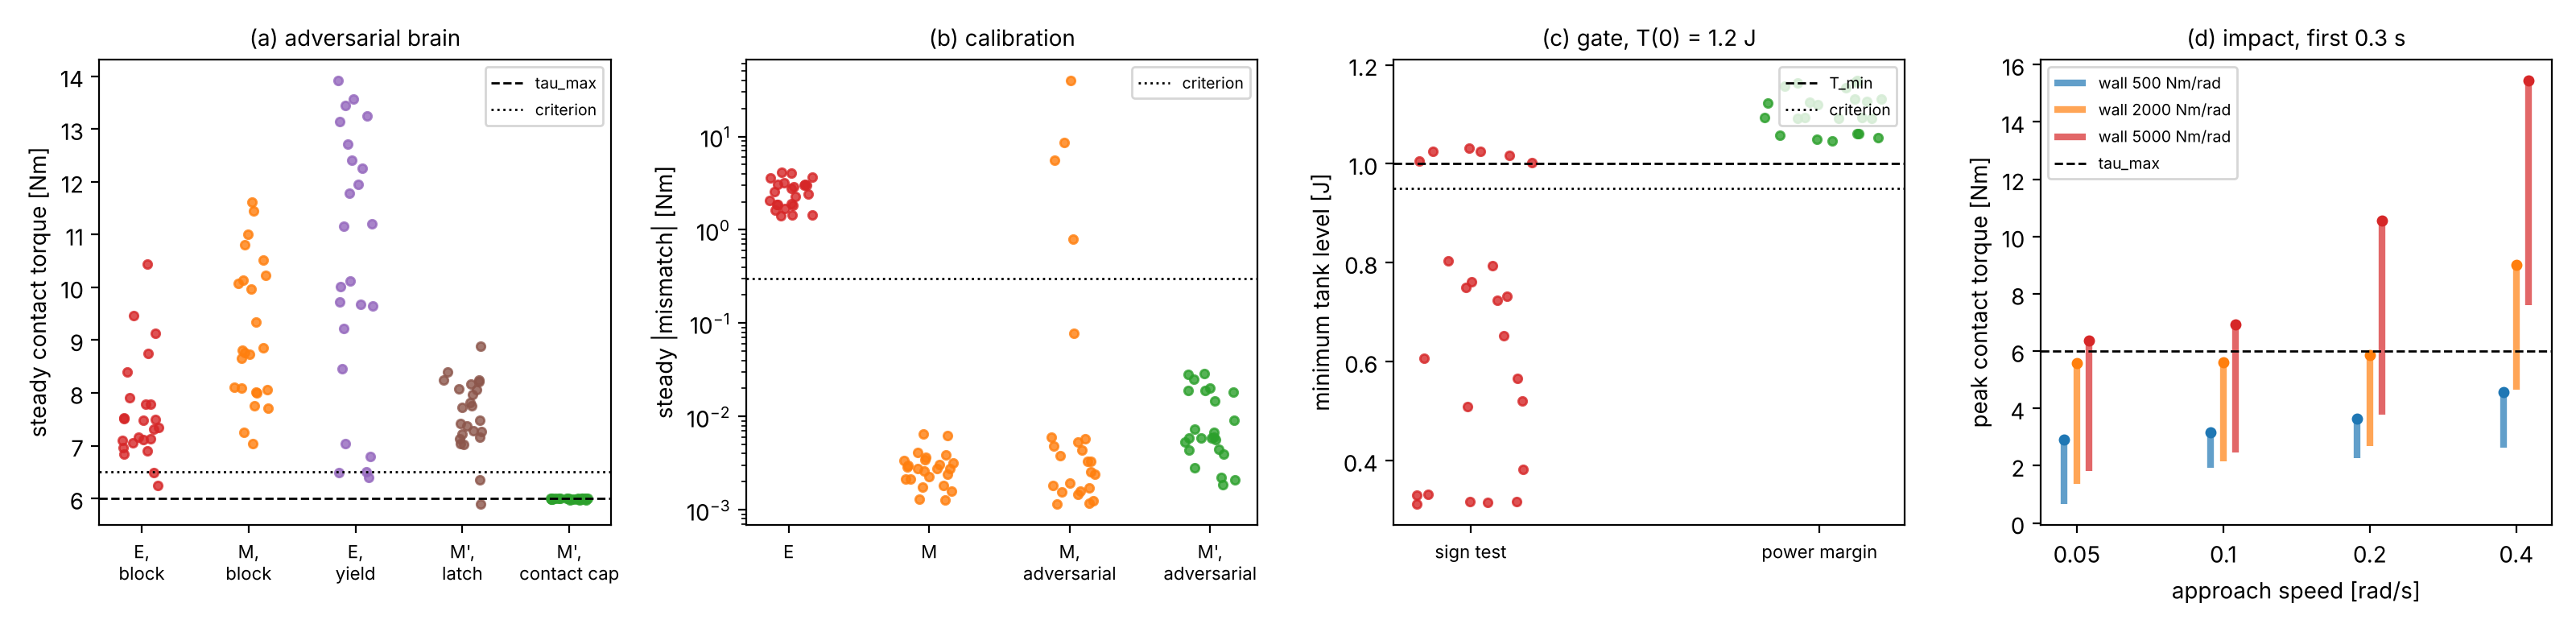
\includegraphics[width=\textwidth]{m1_results.png}
\caption{M1 results}
\label{fig:m1}
\end{figure}

\begin{itemize}
\item \textbf{M1 (사전 등록 해시 2cd695a1).} 예측 P1은 기각되었다. 적대적 뇌에서 정상 상태 접촉 torque(문턱 6.5 Nm)가 명세의 calibration(E)에서 6.238--10.448 Nm, 감지 신호 calibration(M)에서 7.040--11.620 Nm였고, 작은 예산에서 최소 tank 수준(문턱 0.95 J)이 0.3125 J였다. 예측 P2는 성립했다. 정상 상태 mismatch가 M에서 0.0013--0.0064 Nm, E에서 1.416--4.117 Nm였다. 에너지 항등식(최대 상대 잔차 5.57e-08), 전달 에너지, 관절 상자, calibration, 접촉 정확도 시험은 통과했다.
\item \textbf{원인 (M1b def20757, M1c aa45e205).} Gate: 작은 예산에서 $T_{\min}$ 아래로 내려간 tank 감소 8.4084 J 전부가 $\alpha=1$인 step, 즉 표본 시점의 부호 판정이 주입을 놓친 step에서 나왔다. M의 windup: 적대적 뇌에서 mismatch가 최대 39.864 Nm까지 커졌고, 그런 run은 모두 접촉 중 saturation을 겪었다. 정지 상태에서 $Ke_q-\hat\tau_{\mathrm{ext}}$가 mismatch와 같다는 관계는 가한 torque가 손의 torque와 같을 때만 성립한다. Guard: 한 step의 spring 증가가 크다는 예측은 기각되었고(최대 0.349 Nm), 벽의 감쇠를 임계값으로 높이면 초과가 대부분 사라졌다(최대 6.909 Nm, 24개 중 3개가 6.5 Nm 초과). 접촉 진동의 골에서 guard가 풀리며 목표가 조금씩 전진하는 것이 주된 원인이다. 양보 guard와 latch guard는 실패했다.
\item \textbf{수정된 구성 (M1d b492b6ae, 모든 시험 통과).} 세 가지를 바꾼다. 감지 신호 calibration은 가한 torque로 계산한다.
\[
\dot z_a=-G_W\Big(\dot q+\kappa\lambda_sK^{-1}\big(u_{\mathrm{ad}}-\tau-\hat\tau_{\mathrm{ext}}\big)\Big)
\]
감지된 접촉 중에는 spring torque를 $\tau_{\max}$로 제한한다.
\[
\|\hat\tau_{\mathrm{ext}}\|>\tau_{\mathrm{th}}\ \Longrightarrow\ \|Ke_q\|\le\tau_{\max}
\]
Gate는 일률 여유 $p_m=0.5$ W를 두고 주입을 판정한다.
\[
\dot q^\top\tau_h>-p_m\ \Longrightarrow\ \alpha=\operatorname{clip}\big((T-T_{\min})/\Delta T,0,1\big)
\]
결과는 에너지 항등식 잔차 1.46e-09, 관절 위반 0, calibration 비율 0.0124, 접촉 torque 오차 0.0206 Nm, 정상 상태 mismatch 0.0090 Nm 이하, 적대적 뇌의 정상 상태 접촉 torque 5.971--6.002 Nm, 작은 예산의 최소 tank 수준 1.0467 J였다.
\item \textbf{남은 관찰.} (a) 1 ms sampling의 관절 상자 stress 시험에서 gauge가 최대 1.0896까지 1을 넘었으나 관절 위반은 없었다. \Cref{thm:r1}은 연속 시간 결과이며 sampled-data 보장 (R10)은 미해결이다. (b) 작은 예산(1.2 J)에서는 24개 중 0개가 벽에 닿았다 (R9). (c) 첫 접촉 후 0.3 s의 최대 접촉 torque는 접근 속도와 벽 강성에 따라 커졌다. 0.05 rad/s에서 0.666--6.376 Nm, 0.4 rad/s와 5{,}000 Nm/rad에서 7.612--15.450 Nm였다 (R17).
\end{itemize}

\textbf{반영.} 위의 세 수정은 승인되어 \Cref{def:hand}(측정된 mismatch에 의한 calibration, 감지된 접촉에서의 spring torque 제한)와 \Cref{def:fulltank}(일률 여유 $p_m$)에 반영되었다. 일률 여유는 이후 L0에서 없앴다(\Cref{sec:l0}).




\subsection{M2: Stage A 결합 학습의 결과}
\label{sec:m2}

\textbf{직관 (무엇을 확인했나).} M2는 뇌와 손을 같은 rollout에서 함께 학습시키고, 부품을 하나씩 뺀 비교와 역할 지표로 각 부분이 의도한 역할을 맡는지 확인한다. 과제는 학습되었고 보장은 모두 유지되었다. 그러나 역할 학습은 일부 seed에서 실패했고, 그 원인은 spring torque를 접촉 한도에 두고 기억을 약 3 Nm 치우친 상태로 두는 해법이었다(\Cref{sec:m2audit}).

\begin{figure}[H]
\centering
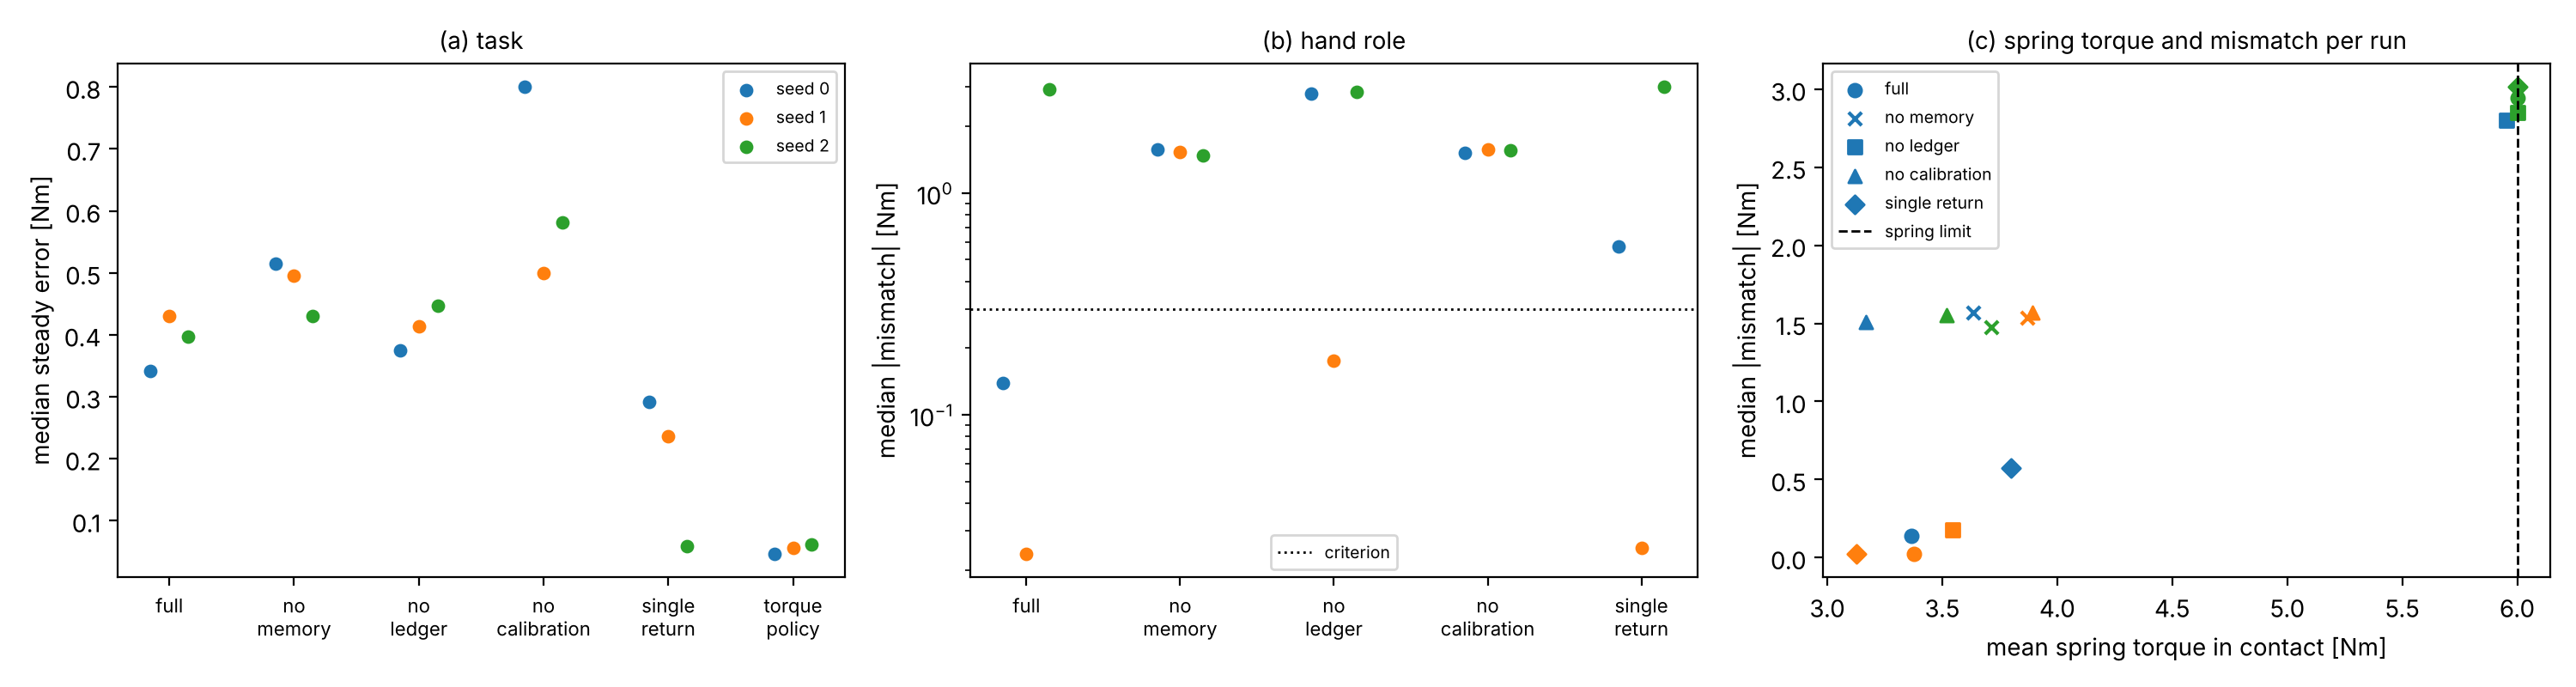
\includegraphics[width=\textwidth]{m2_results.png}
\caption{M2 results}
\label{fig:m2}
\end{figure}

\begin{table}[H]
\centering\footnotesize
\caption{M2 evaluation per arm (seeds 0, 1, 2)}
\label{tab:m2}
\begin{tabular}{lllll}
\toprule
비교 대상 & 정상 상태 오차 [Nm] & mismatch [Nm] & RSI & 장부 의존 [Nm] \\
\midrule
full & 0.342, 0.431, 0.397 & 0.139, 0.024, 2.943 & 0.045, 0.068, -- & 2.658, -0.035, 2.024 \\
no memory & 0.514, 0.496, 0.430 & 1.567, 1.534, 1.475 & 0.940, 0.974, 0.976 & 2.486, 2.504, 1.865 \\
no ledger & 0.375, 0.413, 0.446 & 2.802, 0.176, 2.852 & 0.147, 0.020, -- & 0.000, 0.000, 0.000 \\
no calibration & 0.801, 0.500, 0.581 & 1.510, 1.568, 1.554 & 0.914, 0.982, 0.974 & 0.983, 1.573, 1.577 \\
single return & 0.292, 0.236, 0.059 & 0.573, 0.025, 3.017 & 0.040, 0.072, -- & 1.473, 2.764, 2.941 \\
torque policy & 0.046, 0.055, 0.061 & -- & -- & -- \\
\bottomrule
\end{tabular}
\end{table}

\begin{itemize}
\item \textbf{사전 등록 (해시 2cfbe45e).} 학습 성공 확인(M0)과 보장(V1: 관절 위반 0, 최소 tank 수준 양수)은 성립했다. P2(calibration 통로), P3(손 내부 장부, 3개 중 2개), P4(역할 손실)는 성립했다. P1은 기각되었다. 기억이 없는 비교보다 오차는 모든 seed에서 작았지만, seed 2의 mismatch가 2.943 Nm였다. P5는 기각되었다(seed 2의 spring torque가 모든 과제에서 같아 RSI가 정의되지 않음). P6은 기각되었다(seed 1의 장부 의존 -0.035 Nm). 표현력: torque 정책의 오차(0.046, 0.055, 0.061 Nm)가 모든 seed에서 v3(0.342, 0.431, 0.397 Nm)보다 0.1 Nm 넘게 작았다.
\item \textbf{사후 진단 (주장 아님).} 역할 손실을 받는 세 비교 대상의 9개 run 중 4개에서 spring torque가 접촉 한도 6 Nm에 붙어 있고 mismatch가 약 3 Nm였다. 접촉 torque가 한도에서 mismatch를 뺀 값, 약 3 Nm로 맞춰진 것이다. 같은 seed를 다시 학습하면 기록된 평가가 그대로 재현되었다. 평가 때 calibration을 정지 상태로만 제한해도 seed 2의 mismatch는 2.392 Nm로 남았고 오차는 0.397에서 1.336 Nm로 커졌다. 치우침이 만들어지는 경로는 \Cref{sec:m2audit}에서 가른다.
\item \textbf{사전 등록한 결정.} 역할 학습이 이루어지지 않았으므로(P1, P5) Stage B 전에 학습 장치를 고친다. 손 내부 정보를 뇌가 쓴다는 주장은 지지되지 않는다(P6). 표현력 차이로 tank 안의 학습된 반사 torque를 검토한다. 단, torque 정책은 2 ms마다, 뇌는 50 ms마다 결정하므로 결정 주기의 차이가 이 비교에 섞여 있다.
\end{itemize}


\subsection{M2 점검: 과제와 검증이 아이디어를 시험하는가}
\label{sec:m2audit}

\textbf{직관 (점검의 결론).} M2는 학습 중에도 기구가 작동하고 보장이 유지됨을 보였지만, 아이디어의 주장, 즉 손의 적응이 실행을 맡고 뇌는 의도만 정하며 두 층이 정보를 주고받는다는 주장을 시험하지는 못했다. 과제가 그 장점을 요구하지 않았고, 보장 장치가 거의 작동하지 않았으며, 평가 지표가 역할을 지킨 해법과 역할이 샌 해법을 구별하지 못했다. 학습 분포 밖의 payload에서는 두 해법이 뚜렷이 갈렸다. 아래 수치는 학습된 seed 1(역할 유지)과 seed 2(역할 누수)의 매개변수로 같은 평가 과제 64개를 다시 돌려 얻었고, 기록된 평가와 일치함을 확인했다. \Cref{tab:m2dims}는 M2의 모든 차원과 상수이다.

\begin{table}[H]
\centering\footnotesize
\caption{Stage A dimensions in M2}
\label{tab:m2dims}
\begin{tabular}{p{3.3cm}p{2.3cm}p{9.2cm}}
\toprule
구성 요소 & 차원 ($m=1$; 일반 $m$) & 내용 \\
\midrule
Plant 상태 & $2$; $2m$ & $q,\dot q$; 한 관절, 링크 1.5 kg(0.2 m), 관성 0.05 kg\,m$^2$, payload는 0.4 m, 입력 한계 20 Nm, 관절 상자 $[-0.4,1.0]$ rad \\
Episode마다 모르는 값 & $7$ & payload $[0,2]$ kg, 벽 강성 $[500,5000]$ Nm/rad(log 균등), 벽 감쇠 $[1,5]$, 점성 마찰 $[0.05,0.3]$, 외란 $[-0.5,0.5]$ Nm, 벽 위치 $[0.5,0.6]$ rad, 남은 bias $[-0.05,0.05]$ Nm; 매 step 잡음 표준편차 0.05 Nm \\
측정 & $3$; $3m$ & $q,\dot q,\hat\tau_{\mathrm{ext}}$(한 주기 지연) \\
뇌 관측 & $11$; $6m+5$ & $t/3$, $q$, $\dot q$, $q_d$, $k/100$, $\hat\tau_{\mathrm{ext}}/3$; 장부 $T/T_0$, $\hat m/3$, $\kappa$, $\alpha$, $a$ \\
뇌 행동(50 ms마다) & $3$; $2m+1$ & $q_d^p\in[-0.4,1.0]$, $k^p\in[10,200]$, $\kappa_p\in[0,1]$(sigmoid) \\
뇌 network & $1{,}539$ & MLP 11--32--32--3, tanh, 내부 기억 없음 \\
손 feature network $G_W$ & $168$ & 1--16--8, tanh, 상수 1개 추가: $G_W(q)\in\R^{9}$(일반: $\R^{n_a\times m}$) \\
손 prior $\bar a_W$ & $9$; $n_a$ & 학습 \\
Fast weight $z_a$ & $9$; $n_a$ & episode마다 0에서 시작, $|z_i|\le10$ projection, $H_W=\|z_a\|^2$ \\
손 상수 & -- & 감쇠 3, $\lambda_s=50$, 목표와 강성의 filter 20과 10 s$^{-1}$, $\tau_{\mathrm{th}}=0.5$, $\tau_{\max}=6$ Nm \\
Tank, gate & 상태 1 & $T(0)=20$, $T_{\min}=1$, $\Delta T=1$ J, $p_m=0.5$ W \\
제약층 & 상태 없음 & $k_1=2$, $k_b=20$, $\rho_{\mathrm{on}}=0.8$, $\rho_{\mathrm{full}}=0.9$ \\
뇌 $\rightarrow$ 손 & $3$; $2m+1$ & filter를 거친 $q_d$, $k$, 그리고 $\kappa$ \\
손 $\rightarrow$ 뇌 & $5$; $m+4$ & $T$, $\hat m$, $\kappa$, $\alpha$, $a$ \\
Torque 정책 & $1{,}249$ & MLP 4--32--32--1, 입력 $(t/3,q,\dot q,\hat\tau_{\mathrm{ext}}/3)$, 2 ms마다 $20\tanh(\cdot)$ \\
학습 & -- & ES, 16 antithetic 쌍 $\times$ 8 과제, 300 반복(run당 3 s episode 76{,}800개), 섭동 0.05와 0.03, Adam 0.02와 0.03 \\
시뮬레이션 & -- & control 2 ms, plant RK4 4 substep, episode 3 s, 비용 구간 $[1,3)$ s, 평가 구간 $[2,3)$ s \\
특권 신호(학습 전용) & -- & 손 손실의 $u^\star(q)$, RSI의 payload \\
\bottomrule
\end{tabular}
\end{table}

\begin{itemize}
\item \textbf{적응이 요구되지 않는다.} 정지 접촉에서 접촉 torque는 기억의 mismatch $m:=u_{\mathrm{ad}}-u^\star$와 spring이 미는 torque $p:=-s(Ke_q)$의 합이다.
\[
|\tau_c|=m+p,\qquad |p|\le\tau_{\max}=6\ \mathrm{Nm}
\]
\[
\Longrightarrow\quad |\tau_c|=3\ \mathrm{Nm}\ \text{is attainable at rest}\iff m\in[-3,9]\ \mathrm{Nm}.
\]
온라인 적응 없이 학습된 prior만 쓴 mismatch는 평가 과제 64개 모두에서 이 구간 안에 있었다(seed 1: $-1.546$--$5.098$, seed 2: $-2.768$--$3.845$ Nm). 감지된 접촉 torque로 목표를 적분하는 뇌는 기억 없이도 목표 힘에 도달할 수 있다.
\item \textbf{의도가 고정되어 있다.} 목표 힘은 모든 episode에서 3 Nm이고 task context가 없어, 뇌는 명령의 사상이 아니라 행동 하나를 배운다. 뇌는 시간 $t$를 입력으로 받고 초기 상태가 고정되어 시간표로 풀 수 있다. 시간 입력을 1.5 s로 고정하면 seed 2의 오차는 0.397에서 0.862 Nm로 커졌고, seed 1은 0.431에서 0.392 Nm였다.
\item \textbf{보장 장치가 거의 작동하지 않았다.} Gate 인자는 항상 1이었고, tank는 20 J 중 17.23 J 이상 남았으며, 제약층은 빠른 접근 순간에만 표본의 1.9\%(seed 1)와 0.6\%(seed 2)에서 작동했다. 관절 한계 근처나 예산이 빠듯한 과제가 없어서, 위반 0은 학습과 보장의 상호작용에 대한 증거가 되지 못한다.
\item \textbf{장부가 정보를 거의 담지 않는다.} $\alpha$는 상수, $T/T_0$는 0.86--1.01, 제약 활동은 거의 0이고, $\kappa$는 뇌 자신의 이전 출력이다. 정보가 있는 항목은 $\hat m$뿐이며, 이는 정지 상태에서만 mismatch와 같다.
\item \textbf{핵심 동작이 비용 구간 밖에서 일어난다.} 비용은 $[1,3)$ s에만 매기는데, 첫 접촉 시각의 중앙값은 0.485 s(seed 1)와 0.774 s(seed 2)였다. 접근과 calibration이 비용 없는 구간에서 끝나고, 자유 공간의 위치 정확도는 평가되지 않는다.
\item \textbf{역할 누수의 경로(\Cref{sec:m2}의 진단을 고침).} Seed 2에서 접촉 중 spring torque는 시간의 95.8\%에서 한도 6 Nm에 있었고, 접촉 중 calibration 강도의 평균은 0.0017이었다. 치우침은 접촉 전에 이미 있었다(1 s에서 mismatch 3.087 Nm). 평가 때 두 경로를 끄고 정상 상태의 부호 있는 mismatch를 쟀다.
\[
\begin{array}{lcc}
 & \text{calibration as trained} & \text{calibration at rest only}\\
\text{velocity term on} & -2.943 & -2.392\\
\text{velocity term off} & -1.347 & -0.055
\end{array}\quad\mathrm{Nm}
\]
속도로 구동되는 기억 항과 운동 중의 calibration(정지 상태가 아니면 $\hat m$에 관성 torque가 섞임)이 함께 치우침을 만들었고, 둘을 끄면 calibration은 참값으로 수렴한다. 앞서의 진단(정지 상태에서 calibration을 꺼서 유지)은 불완전했다.
\item \textbf{지표가 역할을 가르지 못한다.} RSI는 spring이 한도에 붙으면 정의되지 않는다. 장부를 0으로 바꾸는 의존도는 입력 분포의 이동을 잰다. 모든 비교 대상이 덜 수렴한 한 시점에서 비교되었다(학습된 v3 0.342--0.431 Nm, M1의 정해진 뇌 0.0206 Nm). Seed는 3개이고, torque 정책과의 비교에는 결정 주기 차이(2 ms 대 50 ms)가 섞여 있다.
\item \textbf{분포 밖 시험이 역할을 가른다.} 학습에 없던 payload 2--4 kg에서 seed 1은 오차 0.381 Nm, mismatch 0.041 Nm를 유지했고, seed 2는 오차 1.963 Nm, mismatch 5.760 Nm로 무너졌다. 학습 분포 안에서는 두 seed의 오차가 0.431과 0.397 Nm로 구별되지 않았다. Annaswamy 등(IEEE TAC 2023)도 적응의 가치를 학습에 없던 불확실성에서 평가했다: 같은 분포 이동으로 학습된 meta-learning 정책은 그 이동에서는 AC--RL보다 나았지만, 학습에 없던 비대칭 propeller 효율 손실에서는 크게 뒤졌다.
\item \textbf{계획과 다르게 실행된 것.} \Cref{sec:plan} 대비: 뇌와 손 모두 evolution strategies(계획: 뇌 PPO, 손은 짧은 구간의 gradient), seed 3개(계획 5개), 뇌와 손의 step 비 0.67(계획 0.1), control 2 ms(계획 1 ms), 학습 범위 밖 시험 없음(계획: 강성 10배까지), 장부 9개 항목 중 5개의 순간값(계획: 구간 평균), task context 없음과 시간 입력 추가, $q$의 잡음과 양자화 없음, 단계 A1만 실행.
\end{itemize}

\textbf{결정 (2026년 11월 13일).} 아래 (a)와 (b)를 승인했다. (b)는 \Cref{def:hand,def:brain,def:ledger,def:rvp}에 반영했다. (a)의 과제는 평면 3관절 팔의 Stage B로 정의했다(\Cref{sec:stageB}).
\begin{enumerate}[label=(\alph*)]
\item 과제 A$'$: episode마다 목표 위치 $q^\star$와 목표 힘 $f^\star$를 task context로 주고, 도달, 유지, 누르기를 한 episode에 담는다. 임의 시각에 payload가 바뀌고(잡기와 놓기), 비용은 episode 전체에 매긴다(유지 중 위치 오차, 누르기 중 힘 오차, 충돌, 에너지). 초기 상태는 무작위이고 시간 입력은 없다. 일부 episode는 목표가 관절 한계 근처이거나 tank 예산이 task energy의 1.2--2배이다.
\item 접점: 뇌의 연속 calibration 강도를 없애고, 손이 감지된 정지 상태에서 스스로 calibration한다. 속도로 구동되는 기억 항을 없앤다(full-power tank와 projection 아래에서 보장은 이 항을 쓰지 않는다).
\item 검증: 역할의 1차 시험은 분포 밖 payload와 강성, episode 중 payload 변화의 회복 시간과 최대 편차, 한 자세에서의 calibration이 다른 자세로 일반화되는 정도, 다른 몸으로 옮긴 뇌의 성능이다. 비교 대상은 같은 결정 주기의 torque 정책과 기억 없는 impedance 정책, 참고용 2 ms torque 정책, recurrent(meta-learning) torque 정책이다. 학습 곡선, seed 5개 이상과 신뢰 구간, 보장 장치의 작동 통계, 정해진 뇌의 상한을 함께 보고한다.
\item 학습: 계획대로 뇌는 PPO, 손은 시뮬레이션을 미분한 짧은 구간의 gradient로 갱신한다.
\end{enumerate}


\subsection{L0: 제어기 부품 시험의 결과}
\label{sec:l0}

\textbf{직관 (무엇을 확인했나).} L0은 학습 없이 정해진 시험용 뇌로 Stage B에서 v3 제어기의 부품을 시험한다. 시험용 뇌는 공칭 기구학과 과제 정보를 쓰지만 $u^\star$는 쓰지 않는다. 사전 등록한 시험에서 두 가지 설계 결함과 두 가지 시험 결함이 드러났고, 고친 구성을 다시 사전 등록해 시험한 결과 모든 관문 기준이 통과했다(\Cref{fig:l0}).

\begin{figure}[H]
\centering
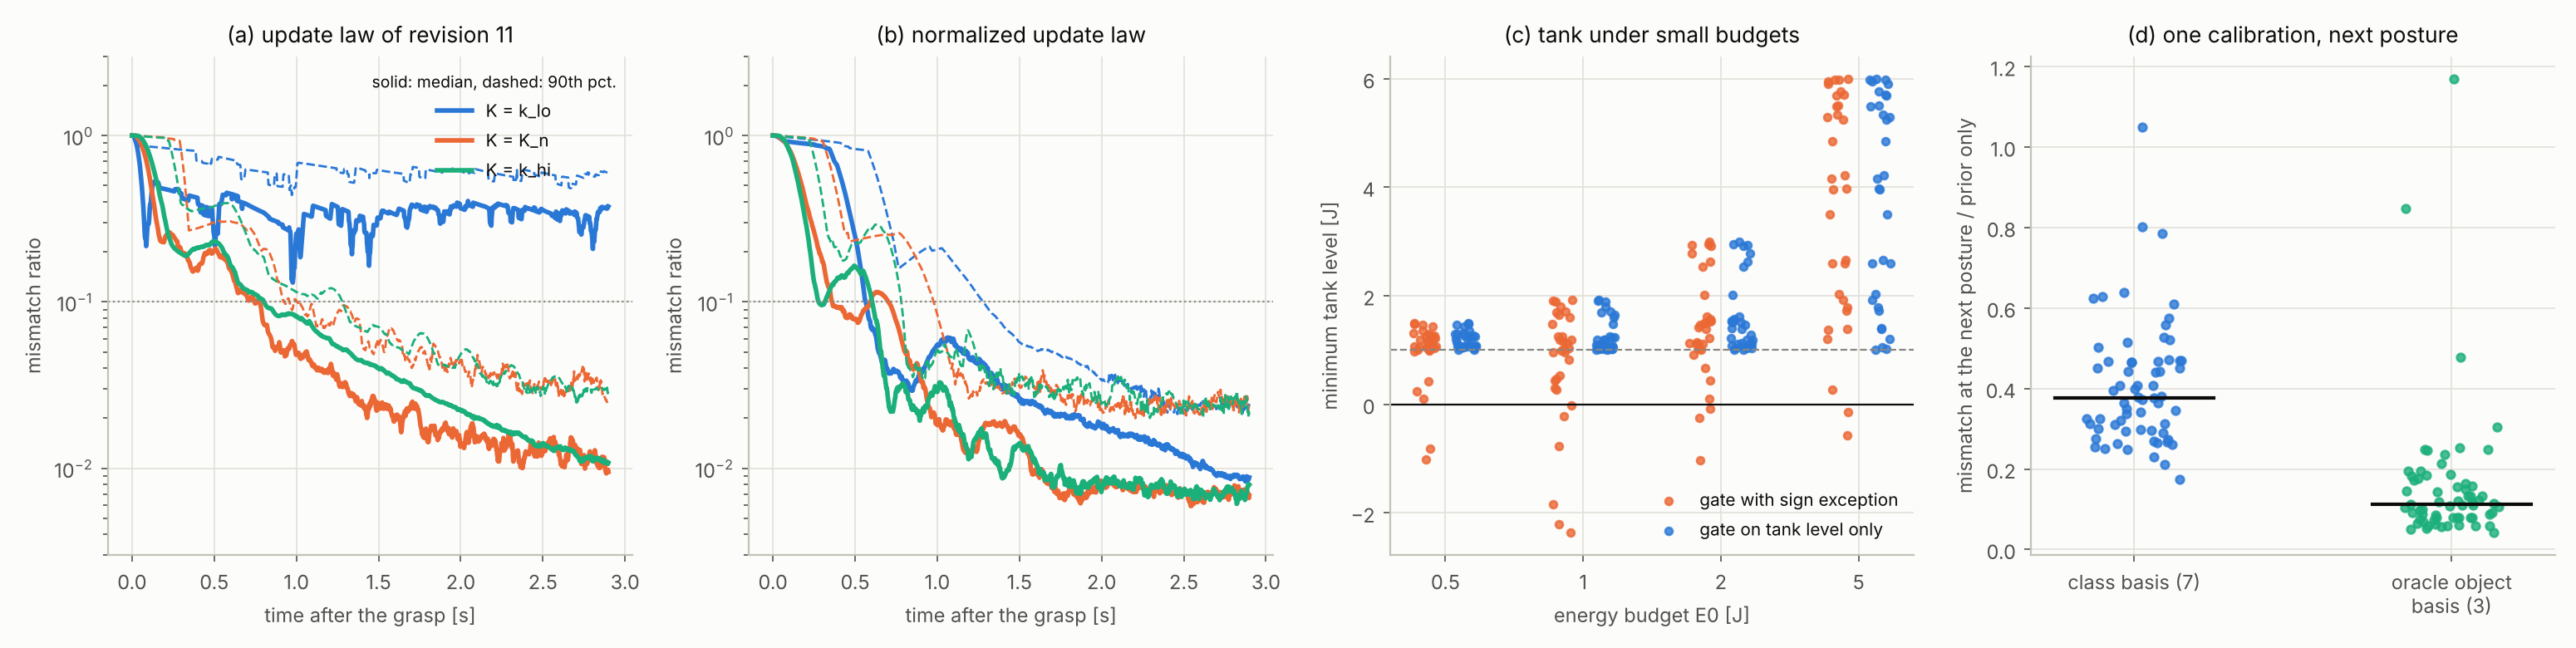
\includegraphics[width=\textwidth]{l0_results.png}
\caption{L0 results}
\label{fig:l0}
\end{figure}

\begin{itemize}
\item \textbf{공학 pilot (주장 아님).} 개정 11의 기억 갱신 법칙 $\dot z_a=-\lambda_s\zeta G_WK^{-1}\hat m$은 정지 판정 없이 돌리면 무거운 물체를 잡은 뒤 주기 약 0.5 s로 진동했다. 이 법칙에서 보정 torque의 변화율은 $-\lambda_sG_W^\top G_W\hat m$인데, class 기저의 $G_W^\top G_W$가 관절 사이를 강하게 결합한다. 그래서 강성이 큰 관절 1의 오차가 관성이 작은 관절 2와 3의 보정을 몰아간다.
\item \textbf{L0 (사전 등록 해시 b3f16fc8).} 관절 상자(모든 $k_b$에서 위반 0), guard, calibration, 정규화 법칙의 기준은 통과했다. $k_b$는 규칙에 따라 2로 정했다. 한계 근처 목표에서 정지 손끝 오차의 중앙값은 $k_b=0.25,0.5,1,2$에 대해 0.001, 0.002, 0.004, 0.006 m였고, 90번째 백분위수는 0.039 m($k_b=2$)였다. 정지 오차는 기억이 barrier를 상쇄하지 않아 생기는 $K^{-1}\tau_b$이다. 실패는 셋이었다. (i) 측정된 관절 각으로 갱신한 tank와 참값의 차이가 최대 0.142 J로 기준 0.1 J을 넘었다. (ii) 작은 예산에서 tank가 0 아래로 내려갔다(보수적으로 계산한 최솟값 -2.359 J). (iii) "개정 11의 법칙이 $K_n$에서 실패한다"는 예측이 기각되었다. 그 법칙은 $K_n$에서 통과하고 $k_{\mathrm{lo}}$에서 실패했다. 일반화 시험은 측정 시점의 결함 때문에 무효였다.
\item \textbf{진단.} (i)은 양자화 효과이다. 부분합으로 정리하면 오차는 $(Q/2)\big(\mathrm{TV}(\tau)+\|\tau_{\mathrm{end}}\|_1+\|\bar u\|_1\big)$ 이하이고, 실제 오차는 이 상한의 0.089배 이하였다. 0.1 J은 유도 없이 정한 값이었다. (ii)는 gate의 예외 규칙, 즉 주기 시작의 일률이 $-p_m$ 이하이면 손을 통과시키는 규칙 때문이다. 떨어지기 시작한 작은 속도에서도 손이 켜지고, 일정한 torque가 주기 안에서 하는 일 $\tfrac12T_s^2\tau^\top M^{-1}\tau\ge0$이 쌓인다.
\item \textbf{L0b (사전 등록 해시 384c4231, 모든 관문 기준 통과).} Gate를 tank 수준에만 의존하게 바꿨다.
\[
\alpha:=\operatorname{clip}\big((T-T_{\min})/\Delta T,\,0,\,1\big)
\]
그러자 작은 예산 128개 run의 최소 tank 수준이 1.0002 J 이상이었다. Tank 오차는 양자화 상한의 0.089배 이하였다. 관절 위반은 0이었고, guard 시험의 정상 상태 접촉 torque는 최대 24.77 N\,m로 상한보다 1.30 N\,m 이상 아래였다. 잡은 뒤 1 s의 mismatch 비율은 중앙값 0.018, 90번째 백분위수 0.069였다. 접촉 시작에 기억을 비운 뒤 1 s에는 중앙값 0.019, 90번째 백분위수 0.044였다(62개 episode). 정규화 법칙의 1 s 비율 중앙값은 $k_{\mathrm{lo}}$, $K_n$, $k_{\mathrm{hi}}$에서 0.051, 0.018, 0.024였고 성장은 최대 0.011였다. 개정 11의 법칙은 각각 0.183, 0.043, 0.082였고, $k_{\mathrm{lo}}$에서 성장 0.64, 최대 속도 1.20 rad/s로 수렴하지 않았다.
\item \textbf{자세 사이의 일반화.} 한 자세에서 1.5 s 보정한 뒤 다음 자세에 처음 정지했을 때의 mismatch를 prior만 쓴 값과 비교했다. 비율의 중앙값은 class 기저(7개)에서 0.377(90번째 백분위수 0.599), 기구학을 쓰는 oracle 물체 기저(3개)에서 0.111(0.247)였다. 예측대로이다. Class 기저는 정확하지만 한 자세의 측정 세 개로 계수 일곱 개를 정하지 못하고, oracle 기저의 나머지는 몸의 편차와 외란에서 온다. 그래서 학습된 regressor $G_W$가 정할 것은 한 번의 보정이 다른 자세로 옮겨 가는 정도이며, 그 기준선은 0.377, oracle 수준은 0.111이다(L2의 역할 시험).
\item \textbf{Sampled-data.} 관절 상자의 stress 시험에서 위치의 gauge는 최대 0.825였지만, 필터링한 속도 $\eta$의 gauge는 최대 2.46까지 1을 넘었다. \Cref{thm:r1}의 불변 집합은 2 ms sampling에서 유지되지 않으며, 관절 위치는 포화된 brake로 지켜졌다 (R10).
\end{itemize}

\textbf{결정 (2026년 11월 14일).} 아래 (a)--(c)를 승인했고 \Cref{def:hand,def:fulltank}와 \Cref{tab:stageB}에 반영했다.
\begin{enumerate}[label=(\alph*)]
\item 기억 갱신을 정규화한다. 그러면 정지 상태의 보정 속도와 안정성이 학습된 feature와 무관해지고, $G_W$는 보정이 다른 자세로 옮겨 가는 방식만 정한다.
\[
\dot z_a=-\lambda_s\,\zeta\,G_W\big(G_W^\top G_W+\varepsilon I\big)^{-1}\hat m\quad\Longrightarrow\quad \dot u_{\mathrm{ad}}=-\lambda_s\hat m\ \ (\varepsilon\to0)
\]
$\lambda_s=5$ s$^{-1}$, $v_r=0.3$ rad/s, $t_r=0.1$ s로 둔다.
\item Gate를 tank 수준에만 의존하게 하고 $p_m$을 없앤다. \Cref{thm:fulltank}(b)의 증명은 그대로 성립하고, 이산 시간의 누수가 사라진다. 대가는 tank가 비면 손의 감쇠도 꺼진다는 것이다.
\item L0의 제어기 상수를 고정한다: $k\in[(50,25,10),(400,200,80)]$, $K_n=(200,100,40)$ N\,m/rad, $D=\operatorname{diag}(30,12,2)$ N\,m\,s/rad, $\tau_{\max}=25$ N\,m, $k_b=2$, $|z_i|\le50$.
\end{enumerate}

\subsection{L1 사전 실험: 과제 타당성의 발견과 제안}
\label{sec:l1pilot}

\textbf{직관 (무엇을 확인했나).} L1은 학습 없이 정해진 뇌로 세 가지를 확인한다. 이 구조로 과제를 풀 수 있는가(상한), 손의 적응과 장부의 정보가 실제로 필요한가, 보장 장치가 실제로 작동하는가. 사전 등록 전에 공학 pilot을 돌렸다(seed 3000--3999, 조건마다 64개 episode, 주장에 쓰지 않음, 기록은 \texttt{records/l1\_pilot.json}). Pilot은 과제와 정보 구조의 결함 세 가지를 드러냈다(\Cref{fig:l1pilot}). 사전 등록한 L1은 아래 제안이 결정된 뒤에 돌린다.

\begin{figure}[H]
\centering
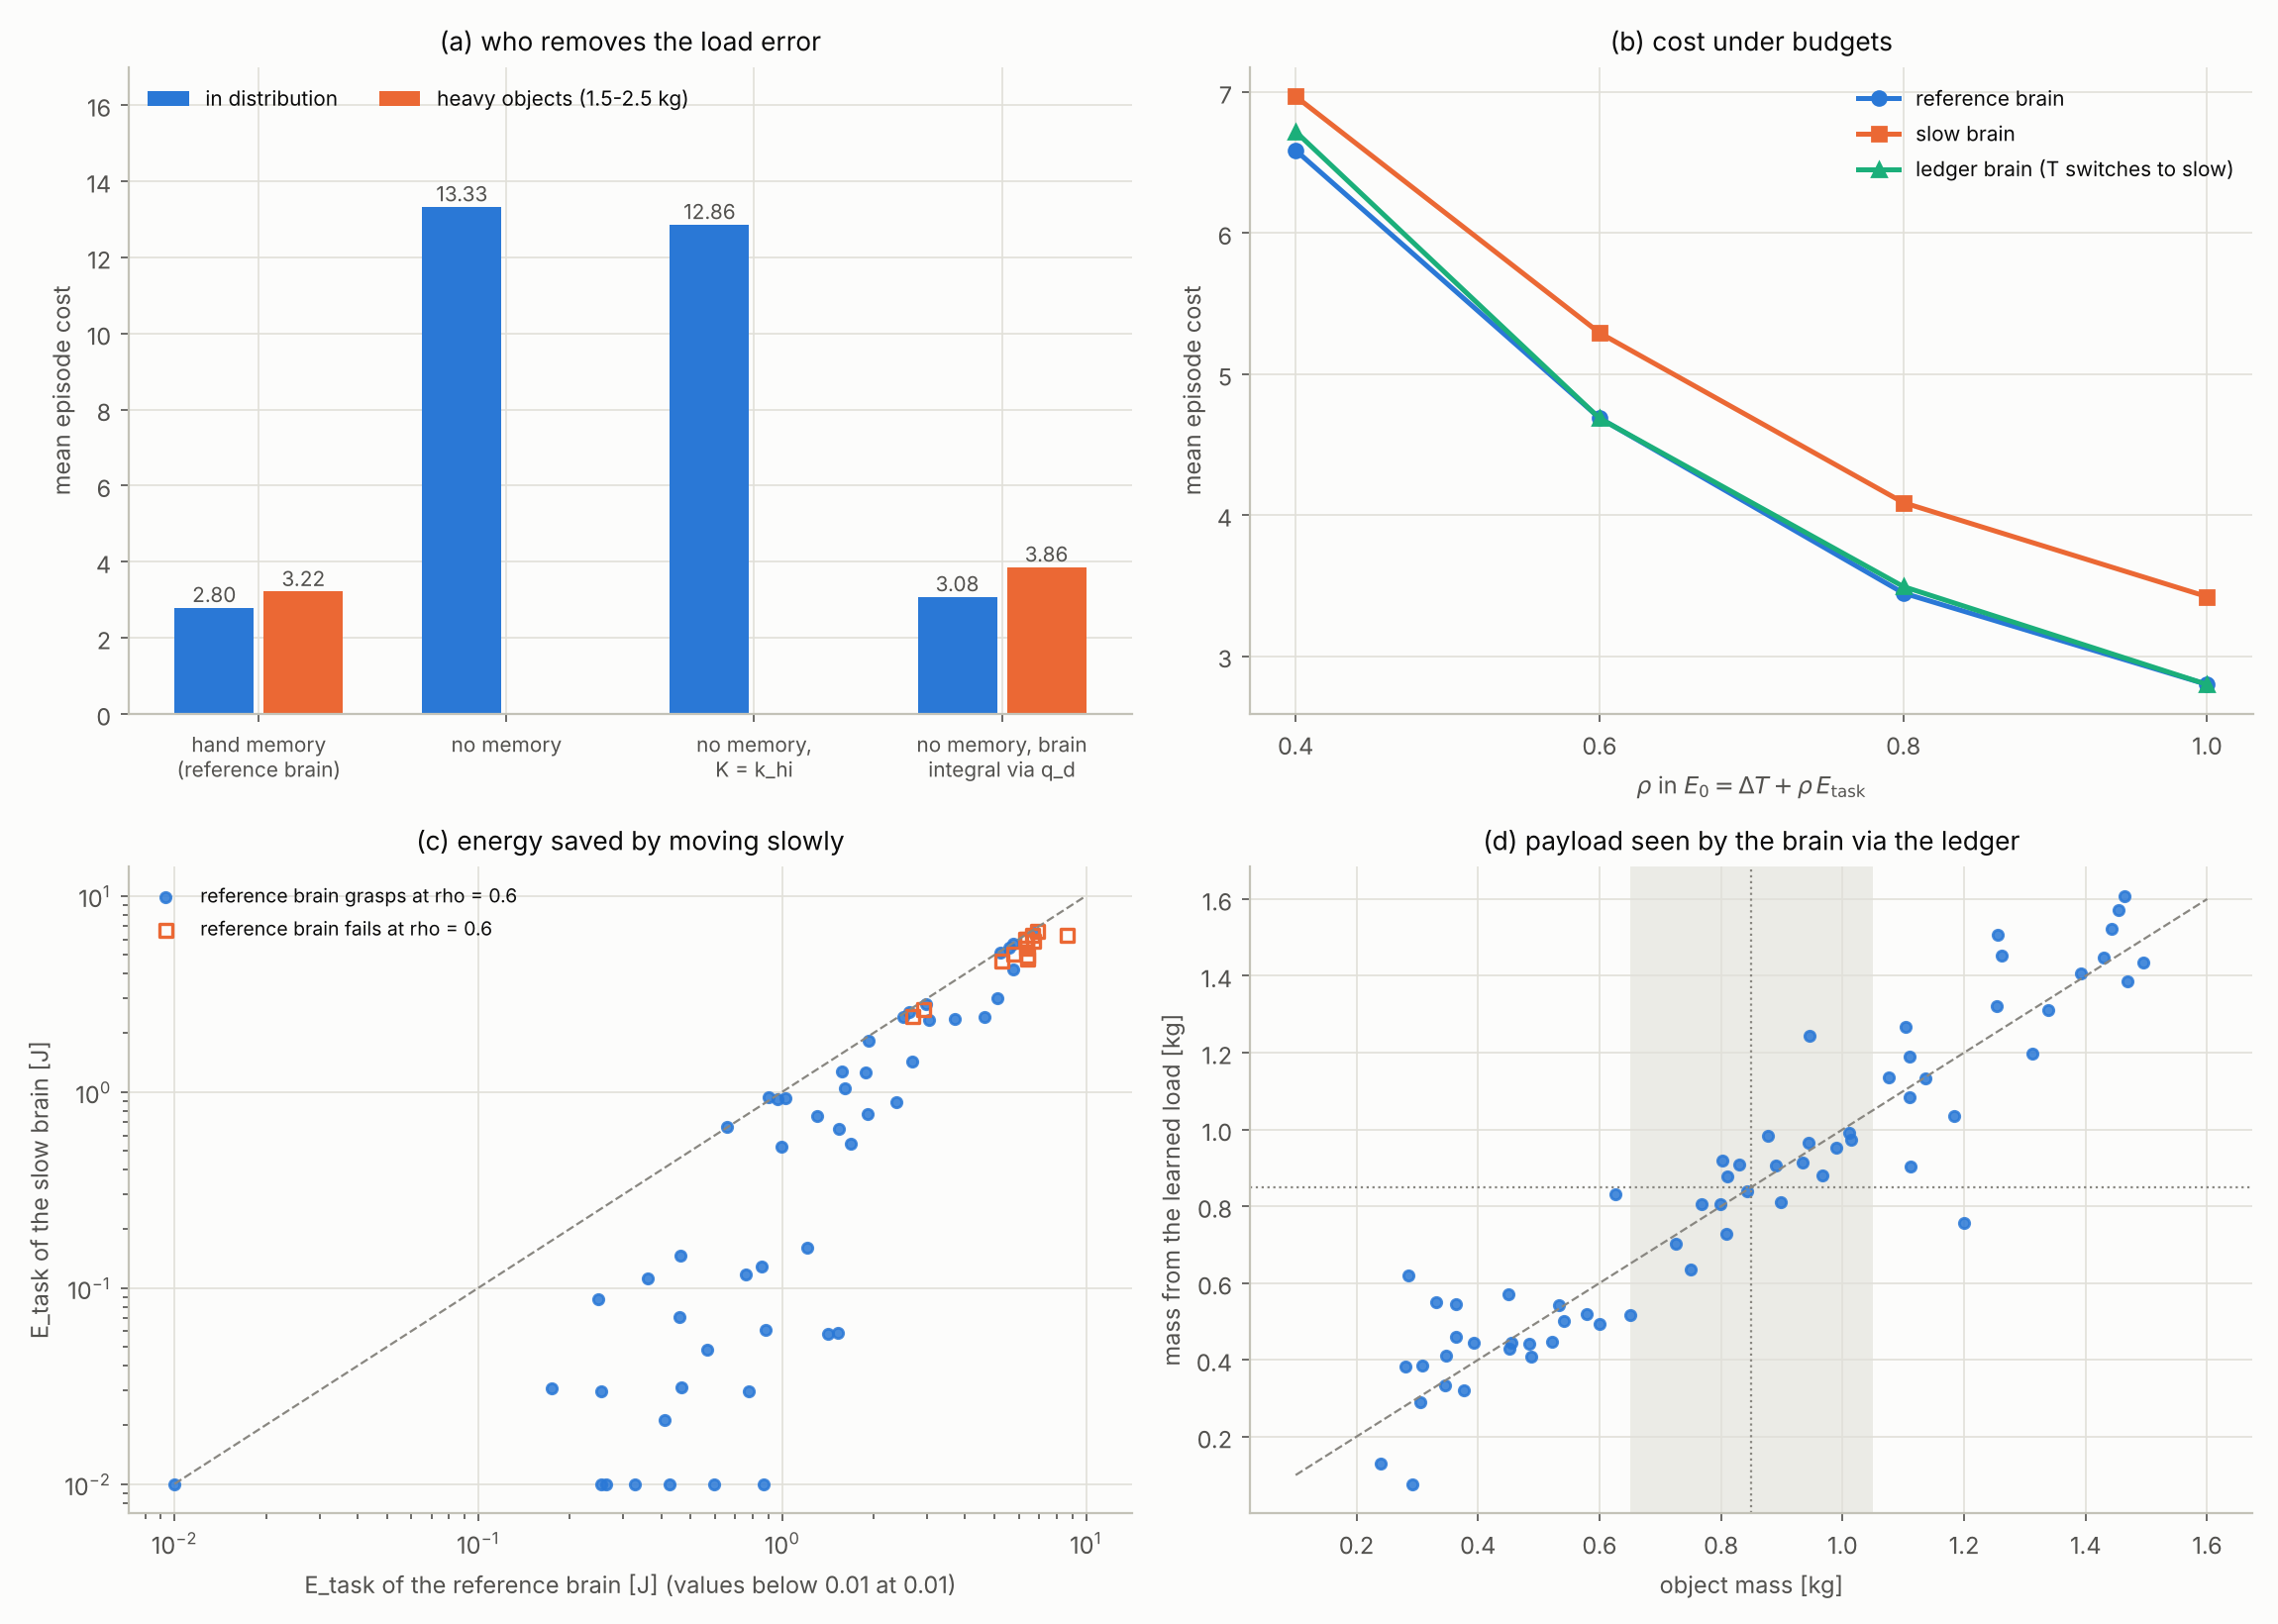
\includegraphics[width=\textwidth]{l1_pilot.png}
\caption{L1 pilot}
\label{fig:l1pilot}
\end{figure}

\begin{itemize}
\item \textbf{시험용 뇌.} 모두 내부 상태가 없는 함수이고 \Cref{def:brain}의 관측만 쓴다. 공칭 기구학의 자세는 과제 정보의 함수이므로 episode마다 미리 계산한다. 기준 뇌는 잡는 점과 목표에서 gauge 여유가 가장 큰 자세로 가고, 잡자마자 목표로 옮기며, 누르기에서는 접촉이 감지될 때까지 내려간 뒤 측정한 자세에서 $K^{-1}J^\top(0,-f^\star)$만큼 떨어진 곳에 목표를 둔다. 중력과 부하의 보상은 손에 맡긴다.
\item \textbf{상한.} 기준 뇌와 v3 손은 모든 episode에서 잡았다. 유지 단계의 위치 오차는 중앙값 0.0003 m, 90번째 백분위수 0.0086 m(한계 근처 목표에서 제약층이 남기는 정지 오차 $K^{-1}\tau_b$), 힘 오차는 중앙값 2.7\%, 90번째 백분위수 9.1\%, 평균 비용은 2.80이었다. 제약층은 hard episode에서 시간의 76.7\%, 나머지에서 8.1\% 작동했고, saturation은 시간의 1.06\%, guard는 64개 가운데 한 episode에서 그 시간의 0.22\% 작동했으며, 관절 위반은 0이었다.
\item \textbf{적응은 필요하지만 뇌가 가로챌 수 있다.} 기억을 끄면 평균 비용이 13.33(힘 오차 중앙값 90.7\%)이고, 강성을 $k_{\mathrm{hi}}$로 올려도 12.86이다. 그런데 기억을 끄고 관측된 실현 목표 $q_d$를 적분기로 쓰는 뇌, 즉 $q_d^p=q_d+g_p(q_t-q)$이고 목표에서 멀면 $q_t$로 바로 가는 뇌는 평균 비용 3.08, 유지 오차의 90번째 백분위수 0.0010 m, 힘 오차 중앙값 4.0\%로 v3 손에 가깝고, 1.5--2.5 kg의 무거운 물체에서도 3.86(v3 3.22)이었다. 뇌가 $q_d$를 보면 정상 상태 보정이라는 손의 몫을 적분 동작으로 대신할 수 있다(역할 누수). $q_d$와 $K$를 쓰지 않는 기준 뇌의 평균 비용은 2.80으로 $q_d$를 쓰는 기준 뇌(2.93)와 비슷하다.
\item \textbf{지금의 예산은 아무것도 시험하지 않는다.} 기준 뇌의 $E_{\mathrm{task}}$는 10번째, 50번째, 90번째 백분위수가 0.34, 1.65, 6.39 J로 gate 폭 $\Delta T=1$ J와 같은 크기이다. 지금의 정의 $E_0=\rho E_{\mathrm{task}}$, $\rho\in[1.2,2]$에서는 $E_{\mathrm{task}}$가 작은 episode에서만 $\Delta T$ 때문에 gate가 걸리고($\rho=1.2$와 2에서 시간 비율 6.7\%와 2.2\%), 평균 비용은 2.82와 2.79로 제한이 없을 때(2.80)와 같다. $E_0=\Delta T+\rho E_{\mathrm{task}}$로 두면 $\rho=1$에서 기준 뇌는 제한을 받지 않고(2.80), $\rho=0.8,0.6,0.4$에서 평균 비용 3.45, 4.69, 6.59, 잡기 91, 78, 69\%, gate 작동 시간 16, 30, 37\%이다.
\item \textbf{장부는 지금 뇌의 결정에 쓰이지 않는다.} Tank 수준이 $T_{\min}+1$ J 아래이면 느리게 움직이는 장부 뇌의 평균 비용은 $\rho=0.8,0.6,0.4$에서 3.49, 4.69, 6.72로 기준 뇌와 같거나 나빴다. 예산 실패는 에너지를 많이 쓰는 episode에 몰려 있다($\rho=0.6$에서 잡지 못한 14개의 $E_{\mathrm{task}}$ 중앙값 6.38 J). 그 에너지는 들어 올리는 데 들고, 천천히 움직여도 중앙값이 5.61 J로만 줄어 14개 가운데 예산 안에 드는 것이 없었다. 여유 자유도로 위치 에너지가 낮은 자세를 쓰면 hard가 아닌 episode의 목표 자세에서 중앙값 1.30 J, 잡는 자세에서 1.53 J를 아끼지만, 단순한 경로로는 옮기는 중에 block 옆면에 걸렸다(평균 비용 7.56). 학습된 부하 $\hat u_{\mathrm{load}}$에서 읽은 물체 질량의 오차는 90번째 백분위수 0.208 kg이지만, 과제에 이 값이 필요한 결정이 없다. 손에서 뇌로 가는 정보는 이 과제에서 쓰이지 않는다.
\item \textbf{분포 밖의 몸.} 링크 길이가 다르면 공칭 기구학의 기준 뇌는 14\%만 잡았다. 손끝 위치의 비례 보정 $q_t+k_cJ^+(p_t-\hat p)$, $k_c=2$로는 73\%(유지 오차 중앙값 0.026 m)였고, 공칭 자세를 향한 적분은 도움이 되지 않았다(12\%). 기구학의 오차는 손이 아니라 뇌가 맡을 몫이다.
\end{itemize}

\begin{fact}[Zero steady-state error needs a hand state]
\label{fact:noint}
Let the memory be off ($u_{\mathrm{ad}}$ equal to its prior), let the measurements be noise-free ($n=0$, exact $q$, $\dot q$ and $\hat p$), and let the brain be a $C^1$ map $\mu$ of $o_k=(q,\dot q,\hat\tau_{\mathrm{ext}},\chi,\ell_k)$, i.e. without $q_d$ and $K$. Fix a posture $q_t$ and a context $\chi$. If a rest equilibrium with $q=q_t$, no contact, open gate and inactive constraint layer and saturation exists for the load torque $u^\star(q_t)$, then
\[
u^\star(q_t)\in\Big\{u_{\mathrm{ad}}(q_t)+K^p(T)\big(q_d^p(T)-q_t\big):\ T\in\R\Big\},
\]
where $q_d^p(T)$ and $K^p(T)$ are the components of $\mu\big(q_t,0,b_\tau,\chi,(T,1,0)\big)$. For $m\ge2$ this set has Lebesgue measure zero in $\R^m$. If $q_d$ is observed, every load admits a rest equilibrium with $q=q_t$ for a suitable $\mu$.
\end{fact}

\begin{proof}
정지 평형에서 $\dot q=0$, $\ddot q=0$, $f_e=0$이고 gate가 열려 있으며 제약층과 saturation이 작동하지 않으므로 $\tau=\tau_h$이고, 운동 방정식에서 $\tau=u^\star$이다.
\[
u_{\mathrm{ad}}(q_t)-K\,(q_t-q_d)=u^\star(q_t)
\]
평형에서는 filter도 멈추므로 $q_d=q_d^p$, $K=K^p$이다(접촉이 없으므로 guard는 작동하지 않는다). 기억이 꺼져 있으므로 $\hat u_{\mathrm{load}}=0$, saturation이 없으므로 $\bar\lambda=1$, 감지된 외력은 $\hat\tau_{\mathrm{ext}}=b_\tau$이다. 따라서 뇌의 관측에서 평형마다 달라질 수 있는 것은 $T$뿐이다.
\[
u^\star(q_t)=u_{\mathrm{ad}}(q_t)+K^p(T)\big(q_d^p(T)-q_t\big)=:c(T)
\]
$c$는 $\R$에서 $\R^m$으로 가는 $C^1$ 사상이므로 국소 Lipschitz이고, 국소 Lipschitz 사상에 의한 $\R$의 상은 $m\ge2$에서 측도 0이다. $q_d$를 관측하면 평형 조건이 $q_d=q_d^p(q_d,\dots)$의 고정점이 된다. 예를 들어 $q_d^p=q_d+g_p(q_t-q)$이면 모든 $u^\star$에 대해 $q=q_t$, $q_d=q_t+K^{-1}\big(u^\star-u_{\mathrm{ad}}\big)(q_t)$가 평형이다.
\end{proof}

\textbf{해석 (무엇이 부족한가).} 지금의 과제에서는 (i) 뇌가 실현 목표를 통해 손의 몫을 대신할 수 있고, (ii) 예산이 기준 뇌를 제한하지 않으며, (iii) 손에서 뇌로 가는 정보가 필요한 결정이 없다. 셋 모두 이 framework의 주장인 역할 분리와 양방향 정보 교환을 시험하지 못하게 만든다.

\textbf{결정 (2026년 11월 14일).} 아래 (a)--(c)를 승인했다. (a)에서 분포 밖의 몸은 기존처럼 질량과 링크 길이를 함께 바꾼다. 질량만 바꾸면 손의 몫을 따로 볼 수 있지만, pilot을 본 뒤 시험 분포를 좁히는 것은 결과에 맞춘 기준 변경이므로 원인은 분석에서 나눈다((P1)).
\begin{enumerate}[label=(\alph*)]
\item 뇌의 관측에서 $q_d$와 $K$를 뺀다: $o_k:=(q,\dot q,\hat\tau_{\mathrm{ext}},\chi,\ell_k)$. 그러면 \Cref{fact:noint}에 의해 정상 상태 보정은 구성에 의해 손의 몫이 되고, 기준 뇌의 성능은 유지된다. 대가는 뇌가 기구학의 오차도 비례 보정으로만 줄일 수 있다는 것이다. 분포 밖의 몸 시험에서는 질량만 바꾸고 링크 길이는 공칭으로 두거나, 길이에 대한 오차 허용치를 사전 등록에서 정한다.
\item 예산 episode의 예산을 $E_0:=\Delta T+\rho\,E_{\mathrm{task}}$, $\rho\sim U[0.6,1]$로 바꾼다. 목적은 장부의 가치를 보이는 것이 아니라 학습과 평가에서 gate가 실제로 작동하게 하는 것이다.
\item 손에서 뇌로 가는 정보가 필요한 결정을 과제에 넣는다. 최소안은 누르기의 목표 힘을 물체 질량의 등급으로 정하는 것이다. 과제 정보에 $f^\star_{\mathrm{light}}$와 $f^\star_{\mathrm{heavy}}$를 주고, $m_{\mathrm{obj}}>0.85$ kg이면 $f^\star_{\mathrm{heavy}}$가 목표이며, 물체 질량은 $[0.2,0.65]\cup[1.05,1.5]$ kg에서 균등하게 뽑는다. 환경은 그대로이고 과제 정보와 비용만 바뀐다. 장부가 없는 뇌는 누르기 단계의 순간 관측으로 등급을 알 수 없다. 감지된 외력에 물체의 무게가 들어가지 않고, 잡은 직후의 처짐은 손이 보정하면 사라지기 때문이다. (P3)은 장부의 유무에 따른 등급의 정확도와 비용의 비교로 바뀐다. Pilot에서 $\hat u_{\mathrm{load}}$로 읽은 등급이 틀린 경우는 띠 $[0.65,1.05]$ kg 밖의 44개 가운데 1개였다. 대안은 놓는 위치를 등급으로 정하는 것(block이 둘 필요하고 환경 검증을 다시 해야 함)과 장부의 가치를 주장에서 빼는 것이다.
\end{enumerate}
\Cref{def:brain,def:ledger,def:stageBtask}와 \Cref{tab:stageB}에 반영했고(개정 13), 환경은 다시 검증했다(\Cref{sec:envcheck}). L1의 사전 등록과 결과는 \Cref{sec:l1}에 있다.

\subsection{L1: 정해진 뇌로 본 과제 타당성}
\label{sec:l1}

\textbf{직관 (무엇을 시험하나).} 개정 13의 과제에서 학습 없이 정해진 뇌로 네 가지를 확인한다. (a) 이 구조로 과제를 풀 수 있다(상한). (b) 손의 기억이 필요하다. (c) 질량 등급의 결정에 장부가 필요하다. (d) 보장 장치가 실제로 작동한다. 분포 밖의 조건은 기준 없이 보고하고, L2의 (P1)에서 쓸 배수를 정한다. 사전 등록은 \texttt{records/preregistration\_l1.md}(hash 5abe91f5)이다. 기준 뇌의 비례 보정 $k_c=1$은 수정된 과제의 pilot(seed 3000--3163, 주장에 쓰지 않음)에서 분포 안 평균 비용이 가장 낮은 값으로 정했다($k_c=0,1,2$에서 2.491, 2.489, 2.784).

\begin{definition}[Reference brain]
\label{def:refbrain}
The reference brain is the static map of $o_k$ given by the following rules, with the nominal kinematics and its Jacobian $J$ at the measured posture.
\begin{enumerate}[label=(\roman*)]
\item (Postures) $q_o$ and $q_s$ are the inverse-kinematics solutions of $p_o$ and $p^\star$ of least gauge, computed from $\chi$ before the episode.
\item (Position goals) $q_d^p=q_t+k_cJ^+\operatorname{sat}_{0.05}(p_t-\hat p)$ with $k_c=1$, where $(q_t,p_t)=(q_o,o)$ while $\xi=0$ in $\mathcal I_1$--$\mathcal I_3$, $(q_t,p_t)=(q_s,p^\star)$ while $\xi=1$ in $\mathcal I_1\cup\mathcal I_2$ and throughout $\mathcal I_4$, and $\operatorname{sat}_r$ clips the norm at $r$ m.
\item (Press) In $\mathcal I_3$ with $\xi=1$: before contact is sensed ($\|\hat\tau_{\mathrm{ext}}\|\le\tau_{\mathrm{th}}$), $q_d^p=q+J^+\big(k_x(p^\star_x-\hat p_x),\,-0.15\,v\big)$ with $v=0.3$ m/s while $\hat p_y>p^\star_y-0.045$ m and $v=0.15$ m/s below; afterwards $q_d^p=q+J^+\big(k_x(p^\star_x-\hat p_x),\,0\big)-K_n^{-1}J^\top(0,\hat f)$, with $k_x=0.5$.
\item (Force class) $\hat f:=f^\star_{\mathrm{heavy}}$ if $e_2^\top(JJ^\top)^{-1}J\,\hat u_{\mathrm{load}}>9.81\,m_{\mathrm{th}}$, and $\hat f:=f^\star_{\mathrm{light}}$ otherwise.
\item (Other outputs) $K^p=K_n$; $\psi=1$ in $\mathcal I_1$--$\mathcal I_3$ and $\psi=0$ in $\mathcal I_4$; goals are clipped to $\mathcal C_q$.
\end{enumerate}
\end{definition}

\textbf{사전 등록한 시험.}
\begin{itemize}
\item \textbf{Episode 집합.} 분포 안 256개(seed 4000, $E_0=E_{\mathrm{nom}}$), 같은 episode를 모두 예산 episode로 둔 것(같은 잡음 열쇠, $E_{\mathrm{task}}$는 분포 안 실행에서), 무거운 물체(1.5--2.5 kg), 분포 밖의 몸(\Cref{tab:stageB}), 질량만 분포 밖, 길이만 분포 밖, 단단한 block 각 128개.
\item \textbf{비교.} 장부를 쓰지 않는 뇌는 목표 힘으로 상수 $(1/a+1/b)/(1/a^2+1/b^2)$, $a=f^\star_{\mathrm{light}}$, $b=f^\star_{\mathrm{heavy}}$를 쓴다. 두 등급이 같은 확률일 때 상대 오차 제곱의 기댓값을 최소로 하는 값이다. 손은 v3, 기억을 끈 손, 기억을 끄고 $K=k_{\mathrm{hi}}$로 둔 손이다.
\item \textbf{기준.} (a1) 잡기 $\ge0.95$, (a2) 등급 정확도 $\ge0.95$, (a3) 상대 힘 오차의 중앙값 $\le0.05$, 90번째 백분위수 $\le0.20$, (a4) 유지 오차의 중앙값 $\le0.005$ m, 90번째 백분위수 $\le0.02$ m, (a5) 모든 실행에서 관절 위반과 유한하지 않은 상태 0. (b1) 기억을 끈 두 손의 평균 비용이 v3의 2배 이상, (b2) 그 상대 힘 오차의 중앙값 $\ge0.25$. (c1) 장부를 쓰지 않는 뇌의 상대 힘 오차 중앙값이 기준 뇌의 3배 이상, (c2) 둘 다 잡은 episode의 80\% 이상에서 기준 뇌의 누르기 단계 비용이 더 낮음, (c3) 장부를 쓰지 않는 뇌의 등급 정확도 $\le0.65$. (d1) hard episode에서 제약층 작동 시간 비율의 평균 $\ge0.30$, (d2) 예산 episode에서 gate 작동 시간 비율의 평균 $\ge0.05$이고 절반 이상의 episode에서 gate가 작동, (d4) 예산 episode에서 $\min_t\big(T-T_{\min}+\max_{s\le t}U_b(q(s))\big)\ge-0.01$ J(\Cref{thm:fulltank}(b), $T_{\min}$ 아래의 saturation이 없는 episode).
\item \textbf{판정 규칙.} 모두 통과하면 L1의 값을 기준으로 L2를 사전 등록한다. (a1)--(a4), (b), (c), (d1), (d2) 중 하나라도 실패하면 원인을 진단해 변경을 제안하고 승인을 받는다. (a5)나 (d4)가 실패하면 구현이나 이론의 오류이므로 먼저 고친다.
\end{itemize}

\textbf{결과 (사전 등록한 기준 모두 통과).} 기록은 \texttt{records/l1\_results.json}과 \texttt{records/l1\_summary.json}이다(\Cref{tab:l1}, \Cref{fig:l1}). 아래 값은 개정 15의 비용(\Cref{def:stageBtask})으로 다시 돌린 것이다. 판정은 모두 같고, 바뀐 값은 평균 비용뿐이다(기준 뇌 2.396에서 2.290, 기억을 끈 두 손 20.775와 20.636에서 11.456과 11.176). 기억을 끈 손은 힘 오차가 커서 누르기 항의 상한에 많이 걸렸다. 개정 13과 14의 기록은 \texttt{records/l1\_results\_rev13.json}, \texttt{records/l1\_summary\_rev13.json}, \texttt{records/l1\_results\_rev14.json}, \texttt{records/l1\_summary\_rev14.json}에 남겼다.

\begin{table}[H]
\centering
\small
\caption{L1 verdicts}
\label{tab:l1}
\begin{tabular}{p{1.0cm}p{7.6cm}p{3.6cm}p{1.2cm}}
\toprule
항목 & 내용 & 값 & 판정 \\
\midrule
a1 & 잡기 성공 ($\ge0.95$) & 1.000 & 통과 \\
a2 & 등급 정확도 ($\ge0.95$) & 0.988 & 통과 \\
a3 & 상대 힘 오차 중앙값, 90번째 백분위수 ($\le0.05$, $\le0.20$) & 0.032, 0.117 & 통과 \\
a4 & 유지 오차 중앙값, 90번째 백분위수 ($\le0.005$, $\le0.02$ m) & 0.0014, 0.0068 m & 통과 \\
a5 & 모든 실행의 관절 위반, 유한하지 않은 상태 (0) & 0, 0 & 통과 \\
b1 & 기억을 끈 손, 끄고 $k_{\mathrm{hi}}$의 평균 비용 (v3 2.29의 2배 이상) & 11.46, 11.18 & 통과 \\
b2 & 그 상대 힘 오차 중앙값 ($\ge0.25$) & 0.628, 0.578 & 통과 \\
c1 & 장부 없는 뇌와 기준 뇌의 힘 오차 비 ($\ge3$) & 8.73 (0.279/0.032) & 통과 \\
c2 & 기준 뇌의 누르기 비용이 더 낮은 episode 비율 ($\ge0.80$) & 0.848 & 통과 \\
c3 & 장부 없는 뇌의 등급 정확도 ($\le0.65$) & 0.469 & 통과 \\
d1 & hard episode에서 제약층 작동 시간 비율 ($\ge0.30$) & 0.736 & 통과 \\
d2 & 예산 episode의 gate 작동 시간 비율 ($\ge0.05$), 작동한 episode 비율 ($\ge0.5$) & 0.140, 1.000 & 통과 \\
d4 & 예산 episode의 tank 하한 여유 ($\ge-0.01$ J) & $2.1\cdot10^{-5}$ J & 통과 \\
\bottomrule
\end{tabular}
\end{table}

\begin{figure}[H]
\centering
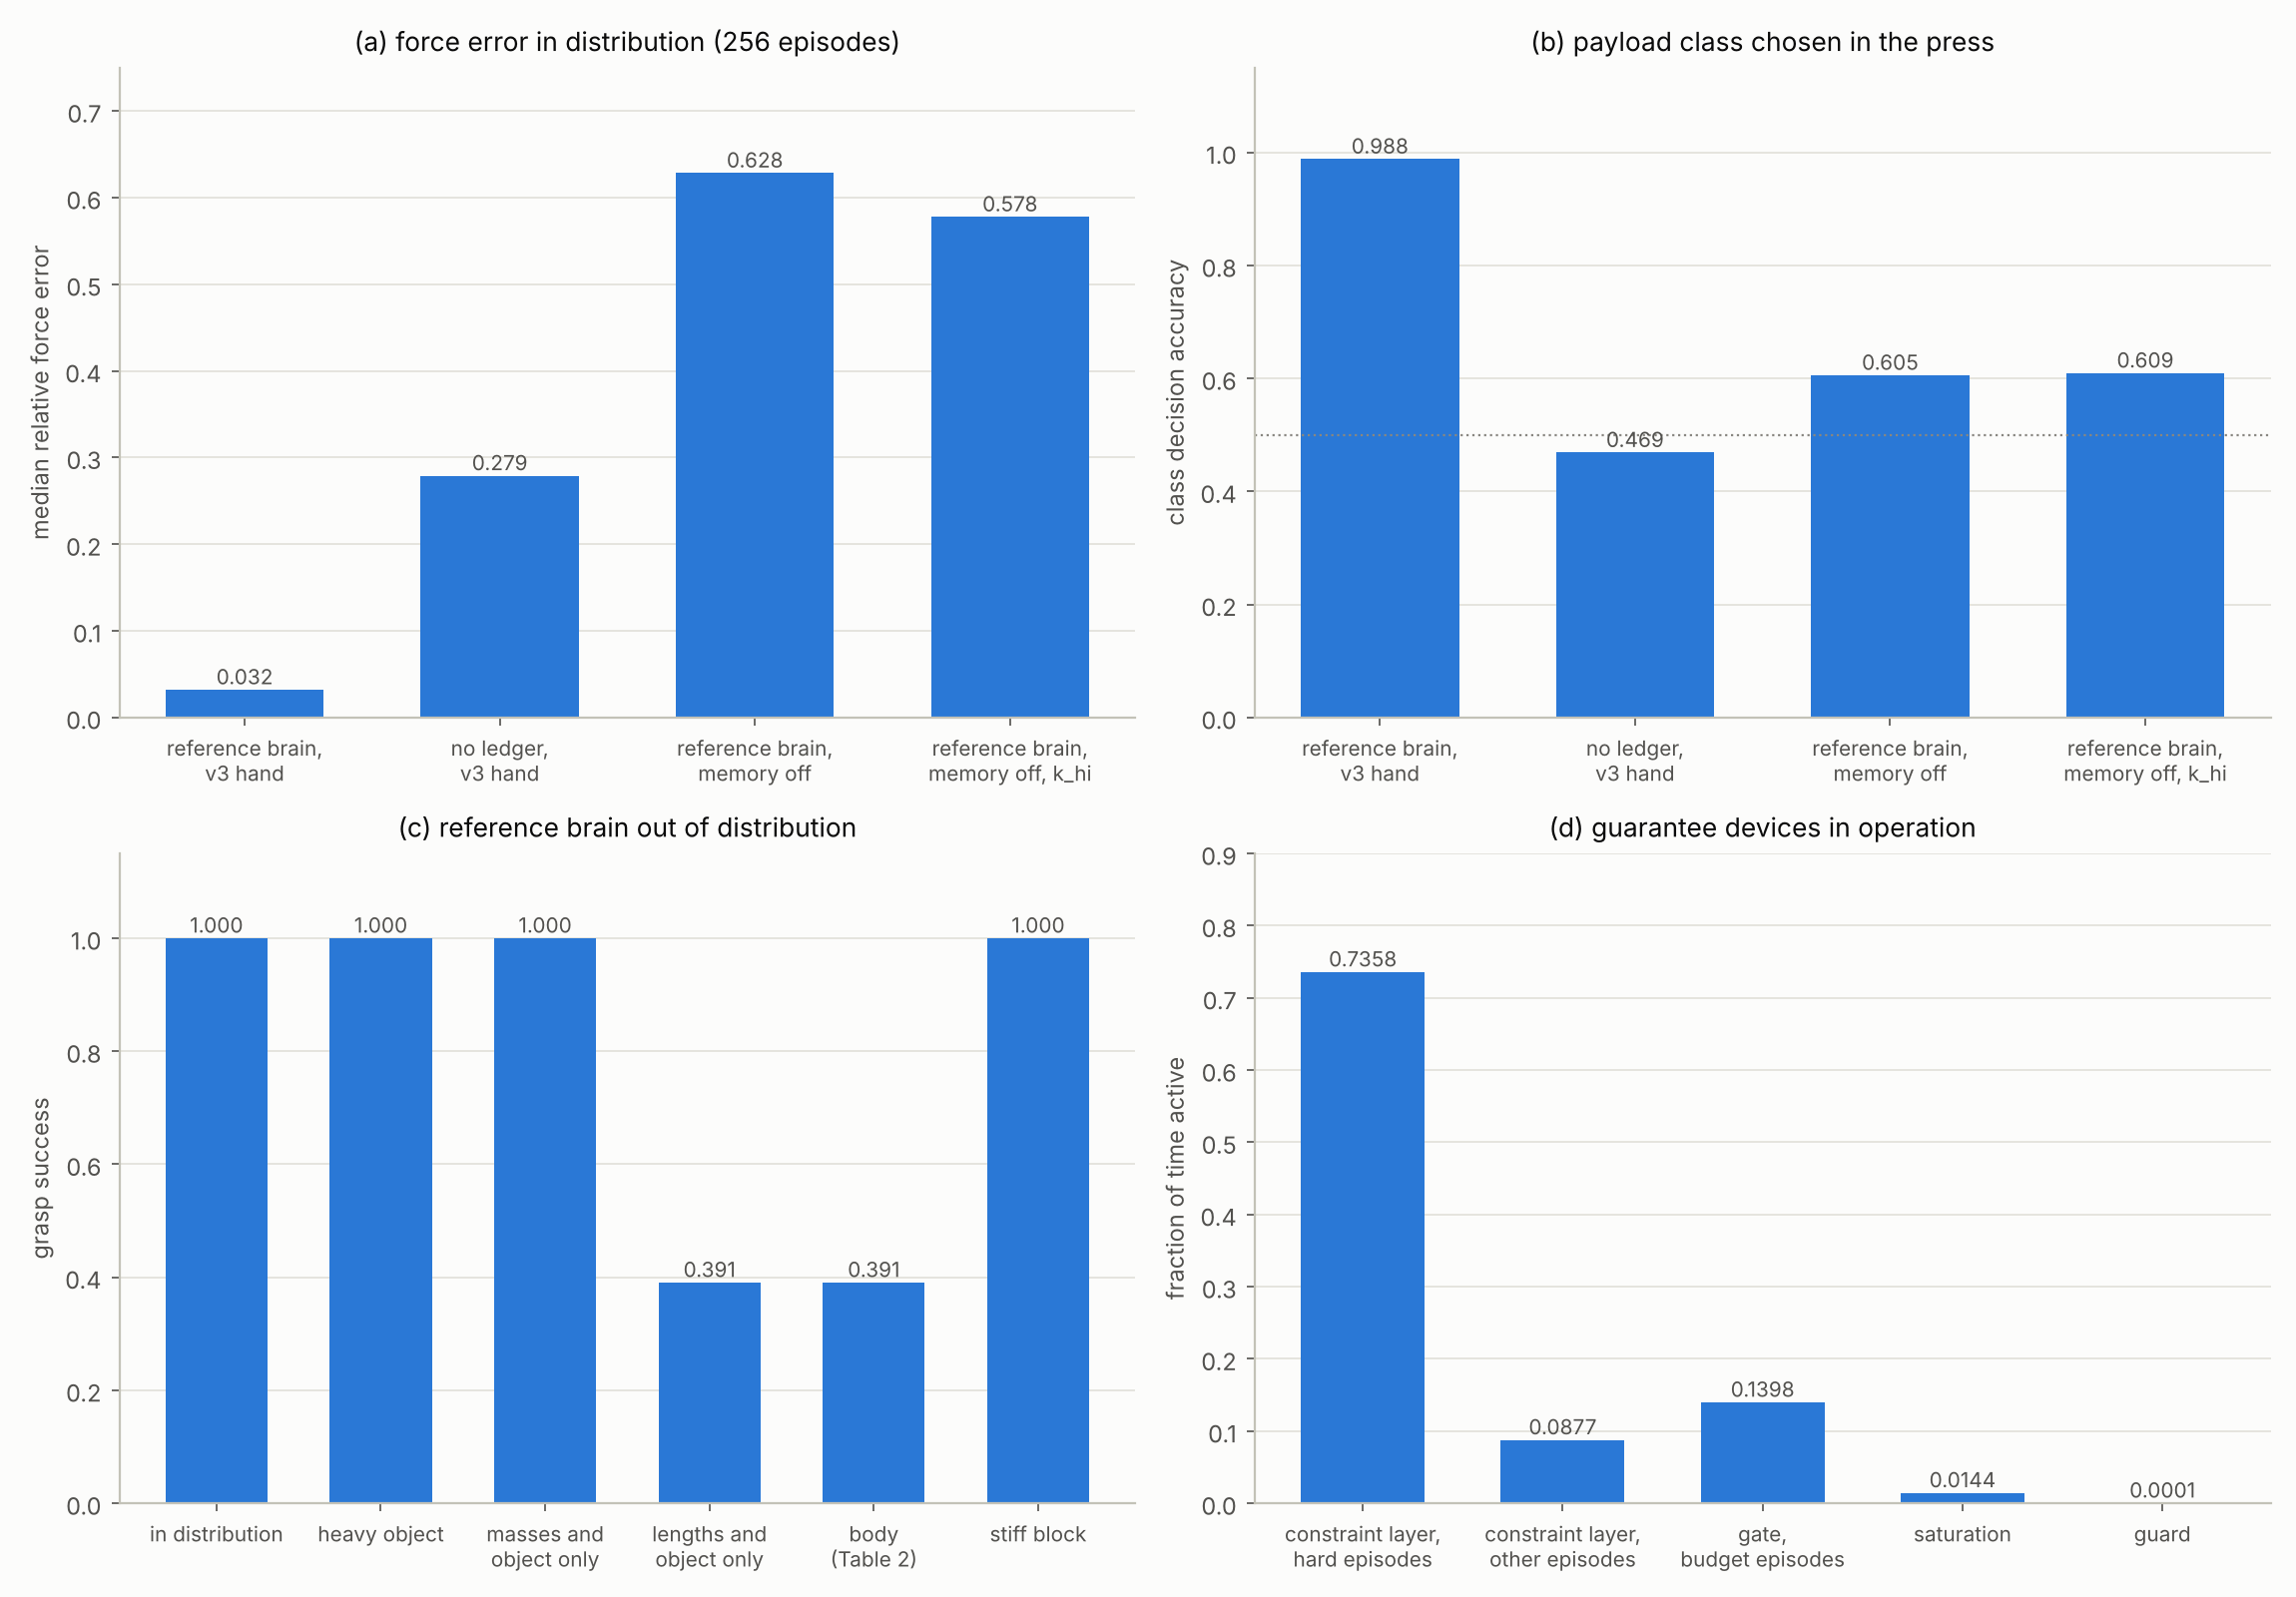
\includegraphics[width=\textwidth]{l1_results.png}
\caption{L1 results}
\label{fig:l1}
\end{figure}

\begin{itemize}
\item \textbf{역할.} 기억을 끄면 강성을 올려도 힘 오차가 0.58 이상으로 남는다. 손의 기억은 강성으로 대신할 수 없고, 뇌는 $q_d$를 보지 않으므로 적분으로 대신할 수도 없다(\Cref{fact:noint}). 등급은 장부가 있을 때 256개 가운데 3개만 틀렸고(질량 1.067--1.103 kg, 무거운 등급의 아래쪽 끝), 장부가 없으면 우연 수준이다. (c2)에서 기준 뇌가 진 39개 가운데 37개는 맞는 목표가 둘 중 작은 힘인 episode였고, 누르기 비용의 차이는 중앙값 0.029로 작았다.
\item \textbf{보장 장치.} 예산 episode의 tank 하한 여유의 최솟값은 $2.1\cdot10^{-5}$ J이고 $T_{\min}$ 아래의 saturation은 없었다. 예산은 평균 비용을 2.29에서 4.02로 올리고 잡기를 0.957로 낮췄다(개정 13의 비용으로는 2.88; 개정 14부터는 잡지 못한 동안에도 물체의 진척 비용을 매긴다). Guard는 분포 안 256개 가운데 21개 episode에서 그 시간의 최대 0.33\% 작동했고, saturation은 시간의 1.44\%였다.
\item \textbf{분포 밖.} 무거운 물체와 질량만 바꾼 몸에서는 잡기 1.000, 평균 비용 2.95와 3.02, 힘 오차 중앙값 0.050으로 손이 몫을 해냈다. 길이만 바꾼 몸과 \Cref{tab:stageB}의 몸은 잡기가 둘 다 0.391이었다. 실패는 링크 길이, 즉 뇌가 맡는 기구학에서 온다. 단단한 block에서는 첫 접촉의 최대 힘이 중앙값 47.9 N(분포 안 15.9 N)으로 커졌다.
\end{itemize}

\textbf{해석 (L2로 가져갈 것).} 개정 14의 과제와 정보 구조에서 (i) 과제를 풀 수 있고, (ii) 손의 기억이 필요하며, (iii) 질량 등급의 결정에 장부가 필요하고, (iv) 제약층과 gate가 실제로 작동하며 tank의 하한이 지켜진다. 위의 값은 L2에서 학습된 뇌를 잴 기준(상한)과 (P1)의 배수를 정하는 데 쓴다. 링크 길이가 바뀐 몸은 기준 뇌로도 잡기가 0.391이므로, (P1)의 몸 부분은 질량과 길이의 하위 조건으로 나눠 판정한다.

\subsection{L2 첫 시도: 결합 학습과 진단}
\label{sec:l2a1}

\textbf{직관 (무엇을 시험했나).} \Cref{def:coupled}를 개정 13의 Stage B에서 seed 하나로 처음 돌렸다. 뇌는 PPO로 task return을, 손은 role loss를 배우고, tank, gate, guard, 제약층은 고정이다. 과제의 성공보다 각 구성요소가 의도한 역할대로 배우는지를 구성요소별로 확인하는 것이 목적이었다. 사전 등록, 실행 중의 수정, 진단, 시험 실행은 \texttt{records/l2\_attempt1\_plan.md}에 기록마다 hash와 함께 있다.

\textbf{구성.} 뇌는 tanh MLP(31--128--128--13)이고, \Cref{def:brain}의 관측에서 다음 넷을 낸다: goal의 평균 $q_d^p=c+h\odot\tanh(u_{1:3})$, 강성의 평균 $k_{\mathrm{lo}}\odot(k_{\mathrm{hi}}/k_{\mathrm{lo}})^{\sigma(u_{4:6})}$(성분별 거듭제곱, $\sigma$는 logistic 함수), 상태에 따른 표준편차(goal은 $[0.005,0.3]$, 강성은 $[0.05,0.5]$), gripper의 logit. Critic(37--128--128--1)은 privileged 입력 여섯 개(단계의 남은 시간, 짐의 질량, 활성 목표 힘, block 깊이, 등급, 예산 여부)를 학습에서만 받는다. PPO는 결정마다 $\gamma=0.99$, $\lambda=0.95$, clip 0.2, 5 epoch, minibatch 4096, 학습률 $3\cdot10^{-4}$, entropy 계수 $10^{-3}$이고, 반복마다 episode 6{,}144개의 pool에서 128개를 뽑는다. 손의 $G_W$는 $(\sin q,\cos q)$의 tanh MLP(6--64--64--21, 성분은 $[-1,1]$)이고 $n_a=7$, $\bar a_W=50\tanh(\cdot)$이다. Role loss는 기록한 rollout 위에서 plant 궤적을 고정하고 \Cref{def:hand}의 기억 법칙을 그대로 다시 돌려 계산한다. Adam(학습률 $10^{-3}$)으로 반복마다 episode 32개씩 16 step을 뇌의 step보다 먼저 한다((L4), $c_r=0$). 10 반복마다 결정적 정책을 episode 64개에서 평가한다.

\textbf{실행 중의 수정 (기록한 뒤 적용).}
\begin{enumerate}[label=(\arabic*)]
\item Goal을 측정 자세에 대한 상대값에서 $\mathcal C_q$의 절대값으로 바꿨다. 상대값에서는 행동 0이 처짐을 따라가 팔이 거의 정지하지 않았고 기억이 보정되지 않았다.
\item Prior의 크기 조정, 손의 step 16, 탐색 잡음의 유지(\Cref{sec:learnplan}).
\item 상태에 따른 표준편차와 상대 위치 입력 $o-\hat p$, $p^\star-\hat p$를 더했다. 기존 입력의 함수이므로 정보 구조는 같다. 반복 70에서 함수를 보존하는 확장으로 이어 학습했다.
\end{enumerate}

\begin{figure}[H]
\centering
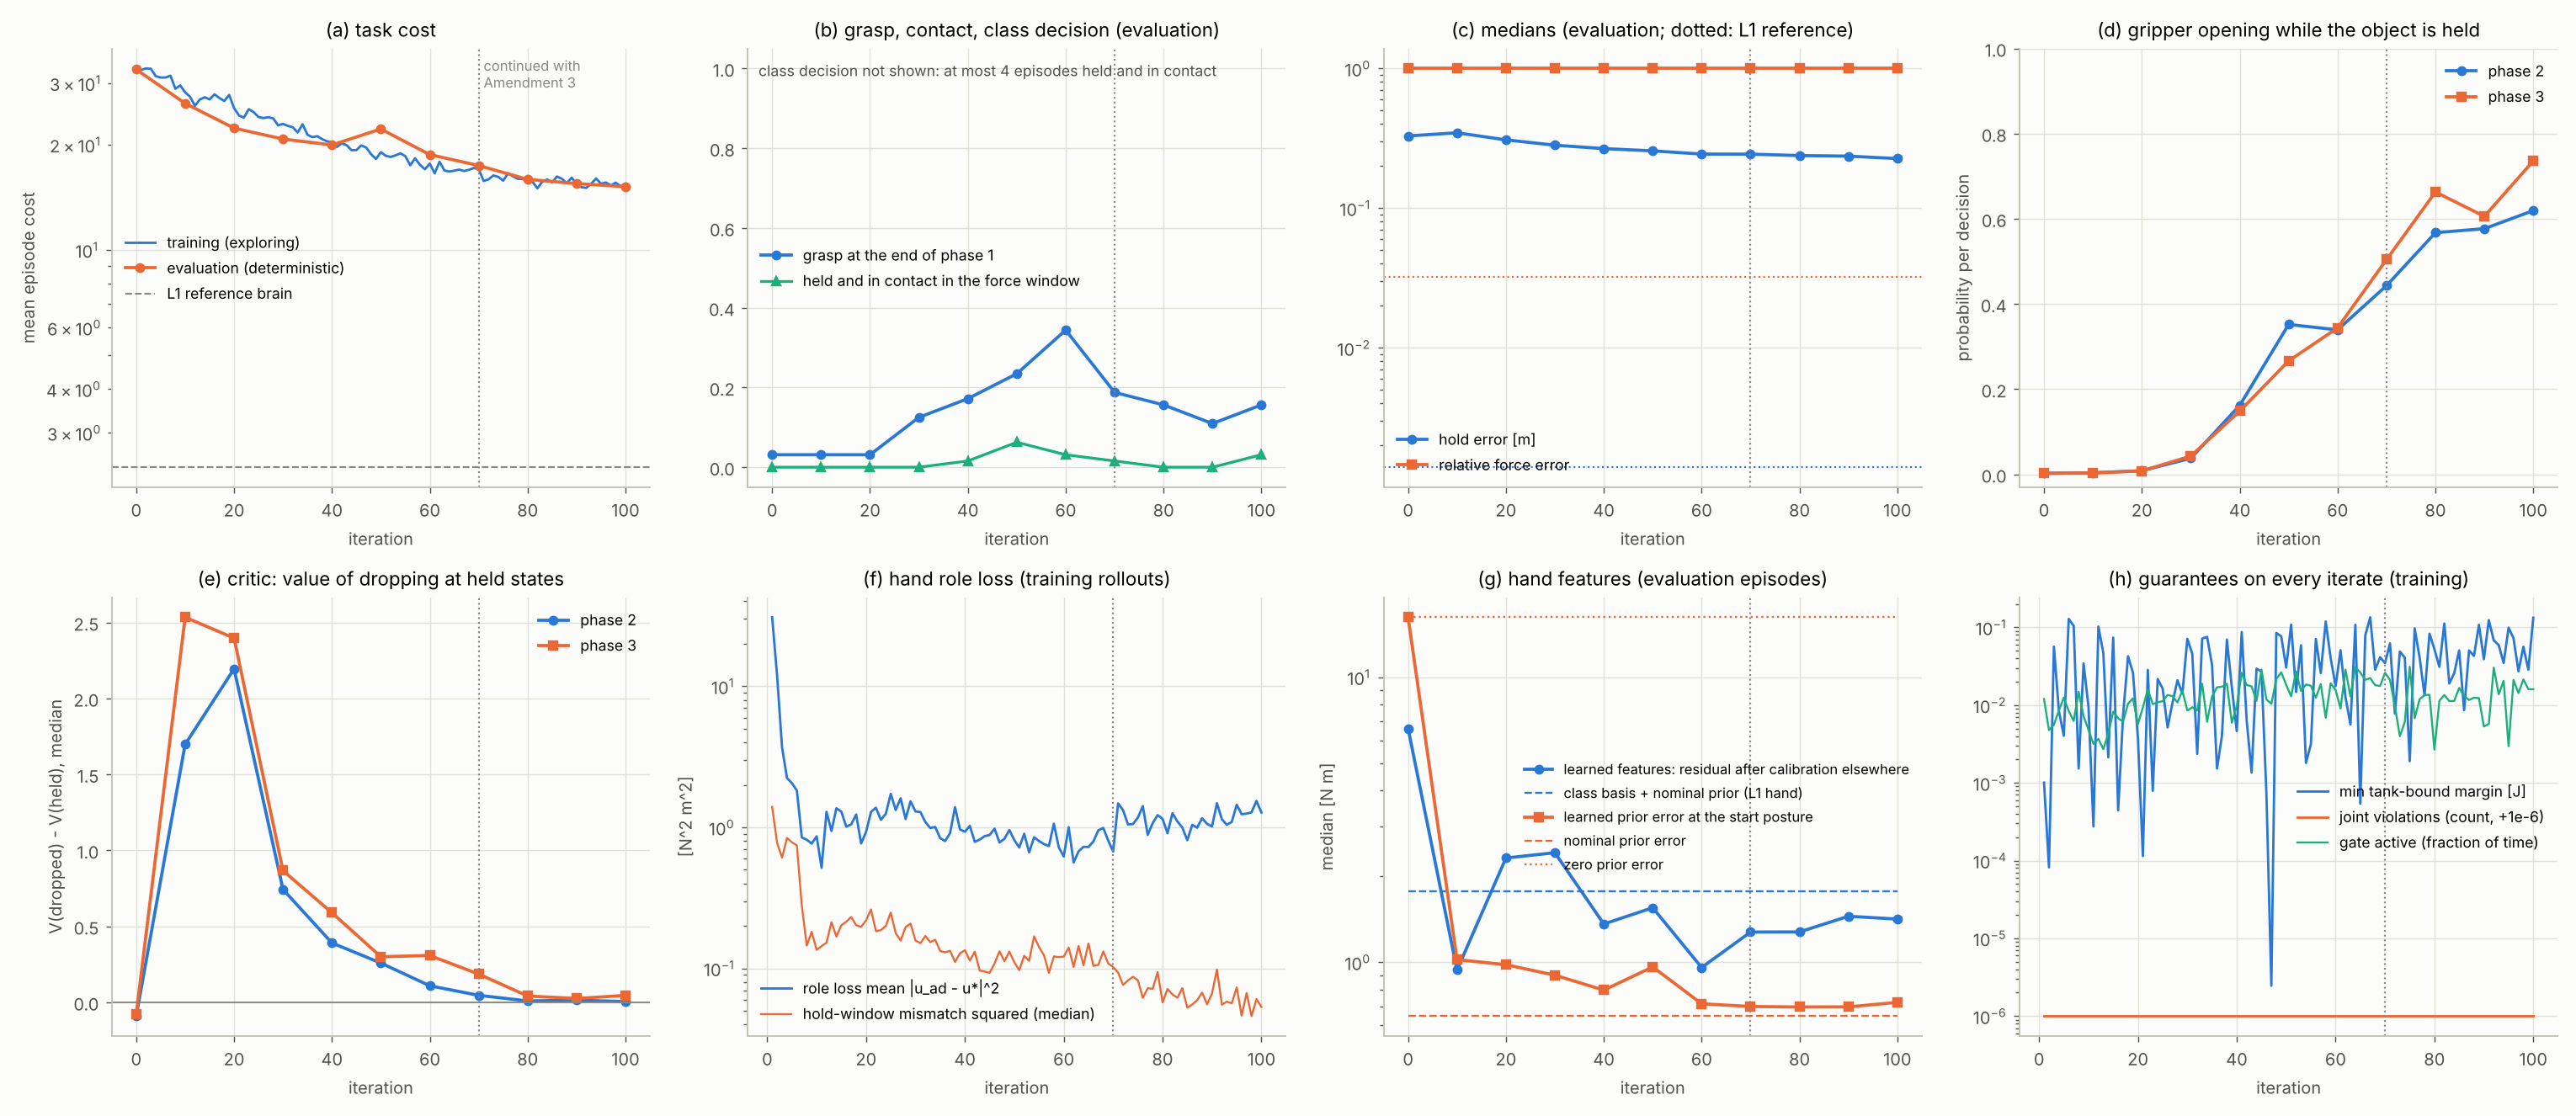
\includegraphics[width=\textwidth]{l2_attempt1.png}
\caption{L2 attempt 1: learning curves and diagnostics}
\label{fig:l2a1}
\end{figure}

\textbf{결과 (반복 0--100, \Cref{fig:l2a1}).}
\begin{itemize}
\item \textbf{보장.} 100번의 반복 모두에서 관절 위반 0, 유한하지 않은 상태 0이고, tank 하한 여유의 최솟값은 $2.5\cdot10^{-6}$ J였다.
\item \textbf{손.} 시작 자세에서 prior의 오차는 영 prior의 16.22 N\,m에서 반복 100에 0.72 N\,m가 되었다(공칭 모형 0.65 N\,m). 한 자세에서 보정한 뒤 다른 자세에 남는 오차는 1.42 N\,m로, class 기저와 공칭 prior(L1의 손)의 1.77 N\,m보다 작다. 반복 80의 학습된 손으로 L1의 기준 뇌를 돌리면 등급 결정 0.984, 상대 힘 오차 0.0313, 유지 오차 0.00157 m, 평균 비용 2.558이고, L1의 손으로는 1.000, 0.0311, 0.00161 m, 2.570이다. 학습된 손은 보상과 장부의 정보원 역할을 모두 했다.
\item \textbf{Critic.} 반복 80에서 단계별 explained variance는 0.965, 0.956, 0.954, 0.972였다.
\item \textbf{뇌.} 반복 80에서 잡는 점까지의 최근접 거리의 중앙값은 0.017 m이고 평가 episode의 58\%가 2 cm 안에 들었다. 그러나 평가의 잡기는 최대 0.344(반복 60)였고, 누르기는 한 번도 없었다(상대 힘 오차 1.000).
\end{itemize}

\textbf{진단 (놓는 것이 이득인 비용).} 학습 rollout에서 뇌는 물체를 잡은 뒤 놓았다. 잡은 상태에서 gripper를 여는 확률은 반복 100에 결정마다 0.619(단계 2)와 0.736(단계 3)이었다. 원인은 개정 13의 비용이다. 개정 13은 놓은 물체의 진척 비용이 없고, 접촉 전의 누르기 항이 $\Pi(p,0)=1+\max\{0,p_y-y_e\}/0.1$이었다.

\begin{fact}[Release incentive under revision 13]
\label{fact:release13}
Under the cost of revision 13, let $t\in\mathcal I_j$ with $f_n(t)=0$, and let $\Omega^1_{\mathrm{task}}$ and $\Omega^0_{\mathrm{task}}$ be the rates with the object held and released at the same configuration ($o=p$).
\begin{enumerate}[label=(\alph*)]
\item $j=2$ $\Rightarrow$ $\Omega^0_{\mathrm{task}}-\Omega^1_{\mathrm{task}}=1-\|p-p^\star\|/0.1$, which is negative whenever $\|p-p^\star\|>0.1$ m, in particular at the grasp point, where $\|p_o-p^\star\|\ge|p_{o,x}-p^\star_x|\ge0.2$ m.
\item $j=3$ $\Rightarrow$ $\Omega^0_{\mathrm{task}}-\Omega^1_{\mathrm{task}}=-\max\{0,p_y-y_e\}/0.1-|p_x-p^\star_x|/0.1\le0$.
\item $j=3$ and $\xi=1$ $\Rightarrow$ on $\{p\in\R^2:\ p_y\le y_e\}$, $\Omega_{\mathrm{task}}=1+|p_x-p^\star_x|/0.1$, independent of $p_y$.
\end{enumerate}
\end{fact}

\begin{proof}
개정 13의 비용에 $o=p$를 넣는다. 단계 2:
\[
\Omega^1_{\mathrm{task}}=\|p-p^\star\|/0.1
\]
\[
\Omega^0_{\mathrm{task}}=1+\|p-p\|/0.1=1
\]
단계 3:
\[
\Omega^1_{\mathrm{task}}=1+\max\{0,p_y-y_e\}/0.1+|p_x-p^\star_x|/0.1
\]
\[
\Omega^0_{\mathrm{task}}=1
\]
(c)는 $p_y\le y_e$에서 $\max\{0,p_y-y_e\}=0$인 것이다.
\end{proof}

\textbf{뇌가 이 결함을 배운 순서.} 학습 rollout의 잡은 결정마다, 같은 자세에서 놓은 상태의 비용률 1보다 든 상태의 비용률이 컸다(반복 70--100에서 비율 1.00, 중앙값은 단계 2에서 2.26--2.71, 단계 3에서 3.98--4.20). Critic이 먼저 배웠다. 잡은 결정에서 $\xi$만 0으로 바꾼 입력의 value와 원래 value의 차이는 중앙값이 반복 0에 $-0.091$(단계 2)과 $-0.078$(단계 3)이었고, 반복 10에 $+1.698$과 $+2.534$로 모든 결정에서 양수가 되었다. Actor가 뒤따라, gripper를 여는 확률이 반복 10에 0.004와 0.003, 40에 0.162와 0.149, 100에 0.619와 0.736이 되었다(\Cref{fig:l2a1}(d), (e); \texttt{records/l2\_release\_mechanism.json}). 무작위 자세 200{,}000개에서 개정 13은 단계 2의 98.2\%, 단계 3의 100\%의 상태에서 놓는 쪽이 쌌고(차이의 최솟값 $-8.17$과 $-14.05$), block 옆면을 따라 든 상태의 단계 3 비용률이 깊이에 대해 평평했다(기울기 0.01/m, \texttt{records/cost\_audit.json}).

\begin{figure}[H]
\centering
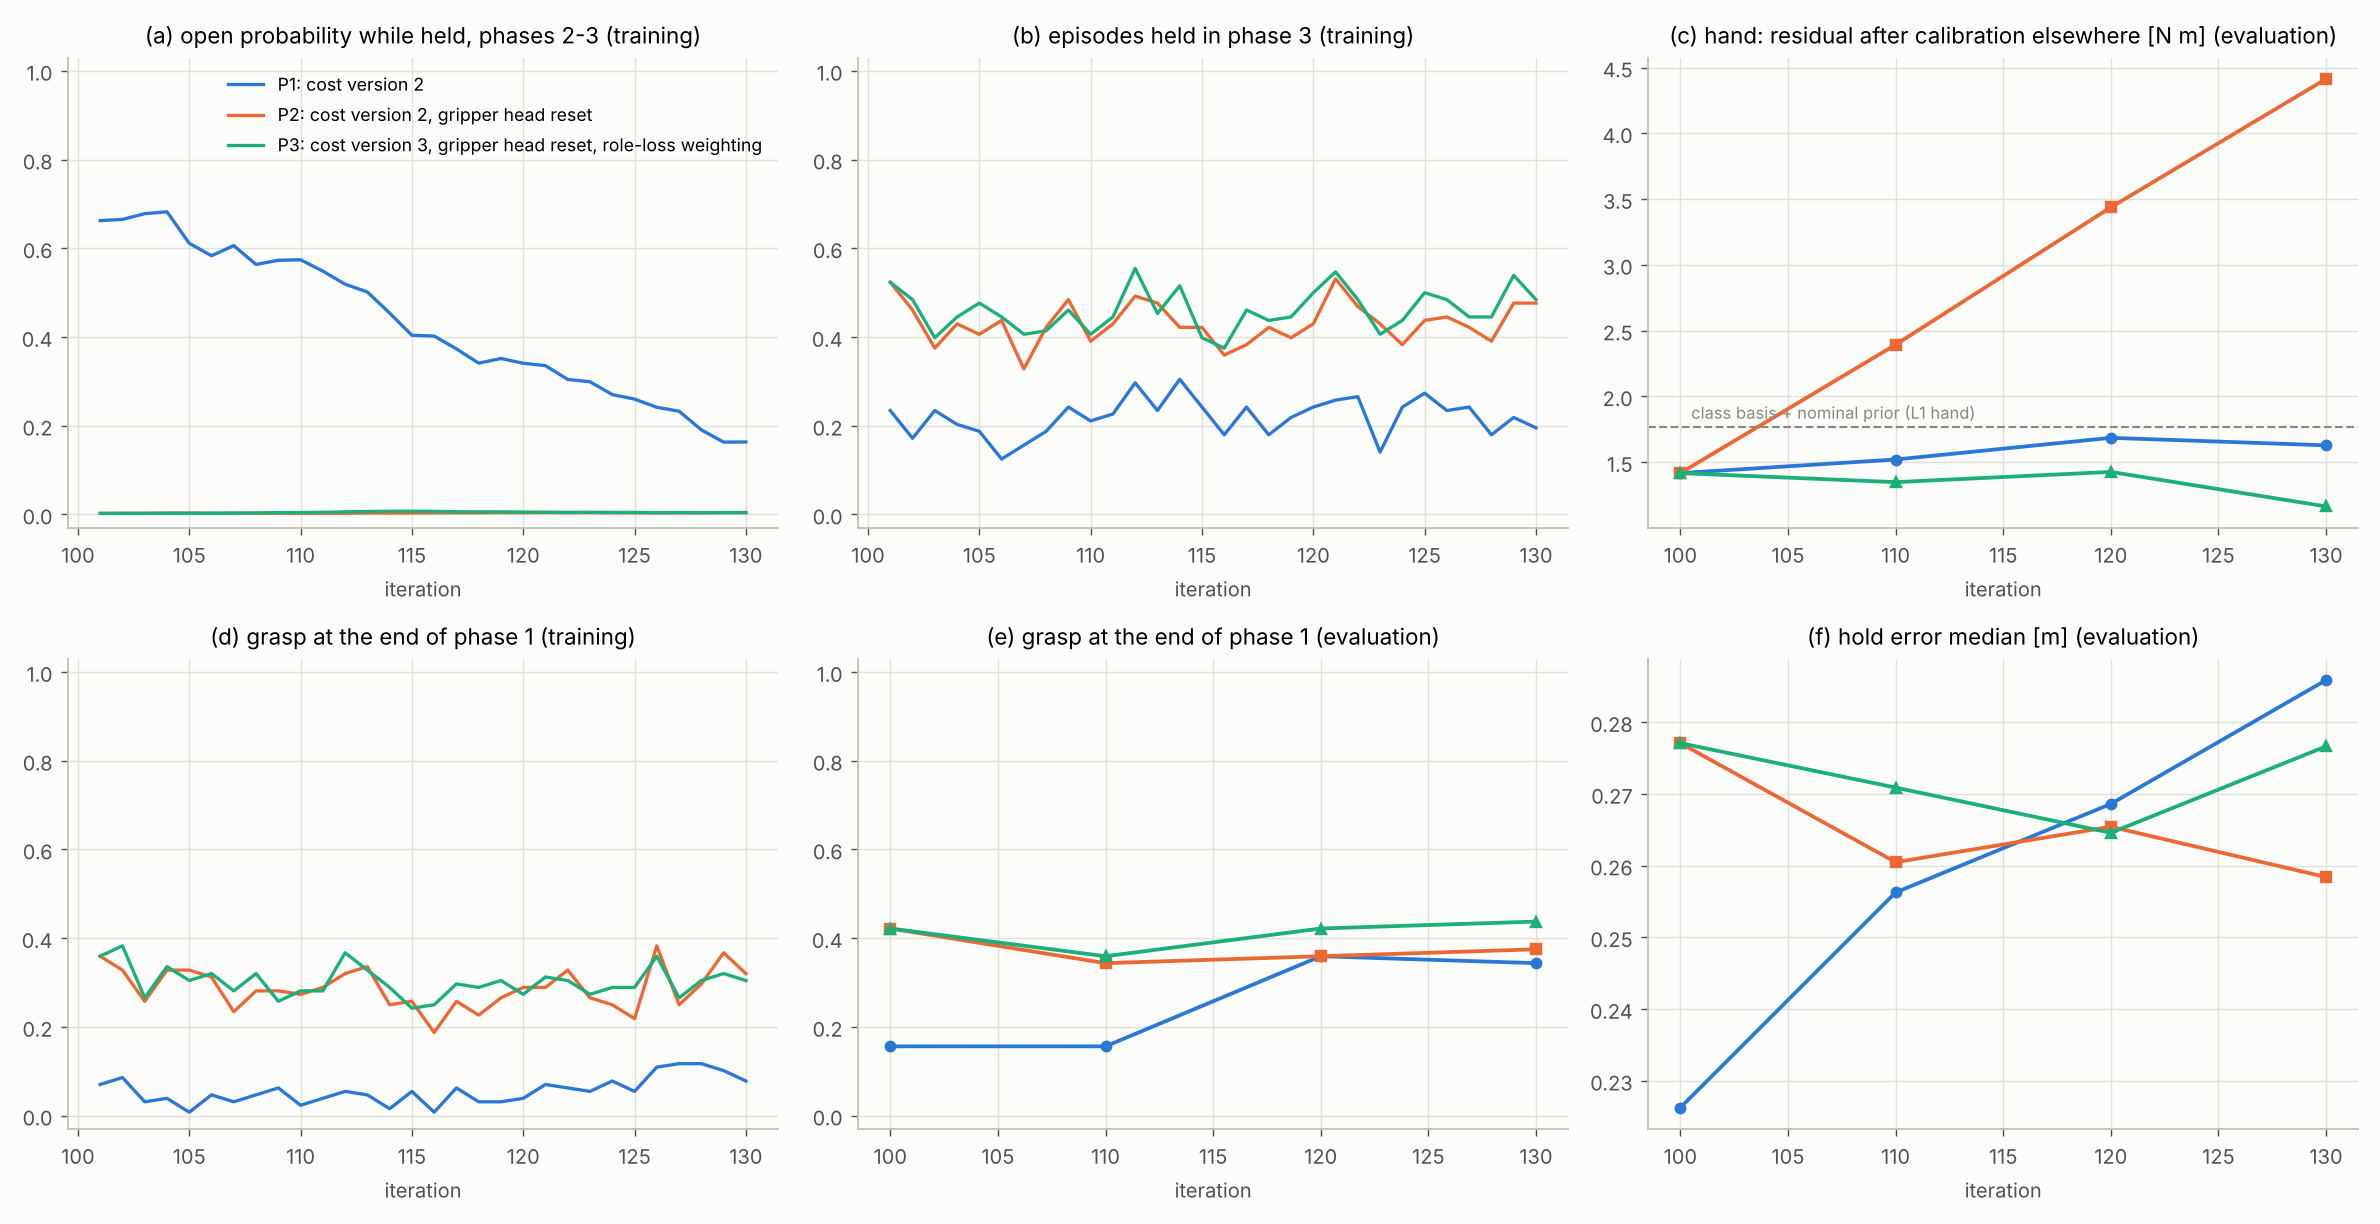
\includegraphics[width=\textwidth]{l2_pilots.png}
\caption{Pilots from iteration 100}
\label{fig:l2pilots}
\end{figure}

\textbf{시험 실행 (반복 100에서 같은 seed로 30 반복씩, \Cref{fig:l2pilots}).}
\begin{itemize}
\item \textbf{P1: \Cref{prop:costprog}(a)를 만드는 비용.} 잡은 상태에서 gripper를 여는 확률이 0.662에서 0.163으로 떨어졌다. 느린 이유는, 놓아도 손끝이 물체 위치에 있어 곧 다시 잡히므로 놓는 대가가 작기 때문이다.
\item \textbf{P2: P1에 gripper head의 초기화를 더함.} 여는 확률은 0.002--0.004, 단계 3까지 든 학습 episode는 0.33--0.53이었다. 새로 두 결함이 드러났다. 첫째, 단계 3에서 든 상태의 시간 가운데 91.5\%가 block 옆면 접촉이었고 윗면 접촉은 0\%였다(윗면 아래 깊이의 중앙값 0.205 m). \Cref{fact:release13}(c)의 평평한 영역이다. 둘째, 손이 나빠졌다. 다른 자세로 옮긴 오차가 4.41 N\,m로 커졌고, 학습된 손으로 돌린 기준 뇌의 등급 결정이 0.719로 떨어졌다. 짐이 바뀐 뒤 기억이 0.1 s 정지하기 전의 구간은 시간의 14.2\%였지만 role loss의 74.2\%를 차지했다(평균 제곱 오차 24.1 대 1.39, \texttt{records/l2\_hand\_share.json}).
\item \textbf{P3: 개정 14의 비용과 가중치에 gripper head의 초기화를 더함.} 다른 자세로 옮긴 오차는 1.16 N\,m, 기준 뇌의 등급 결정은 0.891로, 사전 등록한 0.9에 못 미쳤다. 가중치 없이 잰 오차에서 보정된 구간의 평균 제곱 오차는 0.989로 P2(1.386)보다 작고, 보정 전 구간은 36.6으로 P2(24.1)보다 컸다. 손이 피할 수 없는 오차를 prior로 덮지 않게 된 것이다. 옆면 접촉은 0.834로 기준(0.2 미만)에 못 미쳤다. 단계 2의 끝에서 goal의 손끝이 $p^\star$에서 0.387 m 떨어져 있어 옮기기를 아직 배우지 못했고, 그래서 단계 3이 block 중심에서 먼 곳에서 시작했다(\texttt{records/l2\_carry\_check.json}).
\end{itemize}

\textbf{결정 (개정 14, 2026년 11월 15일 사용자 승인).}
\begin{enumerate}[label=(\arabic*)]
\item \Cref{def:stageBtask}의 비용을 진척 구조로 다시 정의했다(\Cref{prop:costprog}). 의도한 경로의 비용은 같고 L1의 판정도 같다(\Cref{sec:l1}). V17이 두 성질을 수치로 확인한다(\Cref{sec:envcheck}).
\item (L2)의 role loss에 가중치 $w$를 넣었다(\Cref{def:coupled}, \Cref{lem:restfloor}).
\item 두 번째 시도는 초기화에서 시작한다. Gripper head의 초기화와 개정 13에서 학습한 run에서 이어 학습하기는 방법으로 쓰지 않고, P2와 P3는 진단의 근거로만 남긴다.
\item 두 번째 시도는 반복 300의 예산, 기준, 중단 규칙을 사전 등록했다(\texttt{records/l2\_attempt2\_plan.md}).
\end{enumerate}

\textbf{해석.} 첫 시도에서 손의 역할 학습과, 손이 낸 장부로 뇌가 등급을 정하는 정보 경로는 의도대로 작동했다. 보장은 190번의 반복(첫 시도 100, 시험 실행 90) 모두에서 지켜졌다. 뇌의 실패는 구조가 아니라 비용의 결함에서 왔다. 손의 role loss의 귀속 결함은 뇌가 물체를 들기 시작한 뒤에야 드러났고, 각 parameter가 제 역할대로 배우게 하는 학습 체계라는 이 연구의 중심 문제에 속한다.

\subsection{L2 두 번째 시도: 개정 14의 결합 학습}
\label{sec:l2a2}

\textbf{구성.} \Cref{sec:l2a1}의 구성(수정 1--3 포함)에 개정 14의 비용과 role loss의 가중치를 쓰고, 모든 가중치를 초기화에서 시작한다. 예산은 300 반복, 기준은 (G) 모든 반복에서 (C1), (H1) 다른 자세로 옮긴 오차의 중앙값이 class 기저의 1.768 N\,m보다 작음, (H2) 학습된 손으로 돌린 기준 뇌의 등급 결정 0.95 이상이다. 뇌의 지표는 기술만 한다. 중단 규칙은 반복 300에서 평가 episode 가운데 물체를 든 채 힘 구간에서 윗면을 누른 것이 25\% 미만이면 멈추고 분해하는 것이다(\texttt{records/l2\_attempt2\_plan.md}).

\textbf{수정 1 (반복 60, 다시 시작하기 전에 기록).} 사전 등록한 goal 탐색 표준편차의 초깃값 0.04는 첫 시도가 reaching을 배운 뒤 이어 학습할 때의 값이었고, 첫 시도가 초기화에서 reaching을 배울 때의 값은 0.1이었다. 0.04로 돌린 run은 반복 50에서 단계 1 끝의 goal 손끝이 영 행동 자세의 손끝에서 0.106 m, 잡는 점에서 0.219 m 떨어져 있었고, 평가의 잡기는 0.016이었다(첫 시도는 반복 30에 0.197 m, 0.073 m, 0.125). 초깃값을 0.1로 고치고 같은 seed로 다시 시작했다. 다른 가중치의 초기화와 episode 열, 잡음 열이 같으므로, 반복 50의 두 run의 비교가 원인의 판정이다(\texttt{records/l2\_goal\_check.json}).

\textbf{원인 분해 (결정 실험 E1--E5, 각 40 반복, 같은 seed).} 수정 1의 판정에서 다시 시작한 run도 반복 50에 goal 손끝이 잡는 점에서 0.233 m 떨어져 있어(0.04로는 0.219 m), 탐색의 크기는 원인이 아니었다. 남은 차이를 하나씩 바꾼 실험의 결과는 \Cref{tab:l2diag}와 같다. A1은 첫 시도의 초기 network를 함수를 보존해 확장한 것이고, A2는 두 번째 시도의 초기 network이다(\texttt{records/l2\_attempt2\_plan.md}의 수정 2--4, \texttt{records/l2\_goal\_check.json}).

\begin{table}[H]
\centering\footnotesize
\caption{Decisive experiments on the learning of reaching}
\label{tab:l2diag}
\begin{tabular}{p{3.2cm}p{2.0cm}p{1.4cm}p{3.6cm}p{1.3cm}p{1.3cm}}
\toprule
run & 초기 network & 비용 & 그 밖의 차이 & 반복 30 & 반복 40 \\
\midrule
첫 시도 & A1 & 개정 13 & 첫 시도의 code & 0.073 m & 0.062 m \\
E4 & A1 & 개정 13 & -- & 0.101 m & 0.089 m \\
E3 & A1 & 개정 14 & -- & 0.195 m & 0.171 m \\
E5 & A1 & 개정 14 & return 규모의 정규화 & 0.167 m & 0.134 m \\
E2 & A2 & 개정 13 & -- & 0.172 m & 0.167 m \\
E1 & A2 & 개정 14 & 상대 위치 입력의 가중치 0 & 0.176 m & 0.170 m \\
\bottomrule
\end{tabular}
\end{table}

표의 값은 단계 1의 끝에서 goal 손끝과 잡는 점 사이 거리의 중앙값이다. E4는 첫 시도의 반복 0 평가를 정확히 재현했다(평균 비용 32.822).
\begin{itemize}
\item \textbf{비용.} 같은 초기 network에서 개정 14는 reaching의 학습을 늦췄다(E3 대 E4). 반복 30에 단계 1 결정의 critic explained variance는 0.63으로 개정 13의 0.95보다 낮았다(\texttt{records/l2\_adv\_check.json}). 같은 rollout을 두 비용으로 채점하면 평균 비용은 50.41 대 27.72, 표준편차는 11.15 대 9.83이다. 첫 결정에서 critic의 잔차(표준편차 4.47) 가운데 뒤 단계의 길이가 7\%, 잡기 결과가 5\%, episode의 기하와 잡기 결과가 합쳐 11\%를 설명했다(\texttt{records/l2\_value\_check.json}). Global-norm clipping이 actor의 step을 줄이는 비율은 두 비용에서 비슷했다(0.115와 0.104). Return 규모의 정규화(E5)는 거리를 줄였지만 E4에 미치지 못해 채택하지 않았다. 개정 14가 reaching의 학습을 늦추는 경로는 미해결이다.
\item \textbf{초기 network.} 개정 13에서 A1이 A2보다 빨랐다(E4 대 E2). 상대 위치 입력의 가중치를 0으로 둔 A2(E1)는 나아지지 않았다.
\item \textbf{범위.} 모든 비교는 seed 하나에서 나왔다. 사용자의 지시에 따라 seed 반복은 하지 않았다.
\end{itemize}
\textbf{이어 학습 (수정 5).} 두 번째 시도는 사전 등록한 구성에 수정 1을 더해, 다시 시작한 run(\texttt{data/runs/20261115010124/l2\_attempt2b})의 반복 50 checkpoint에서 optimizer 상태와 episode 추출 상태를 새로 두고 300까지 이어 돌렸다(\texttt{data/runs/20261115010124/l2\_attempt2}).

\begin{figure}[H]
\centering
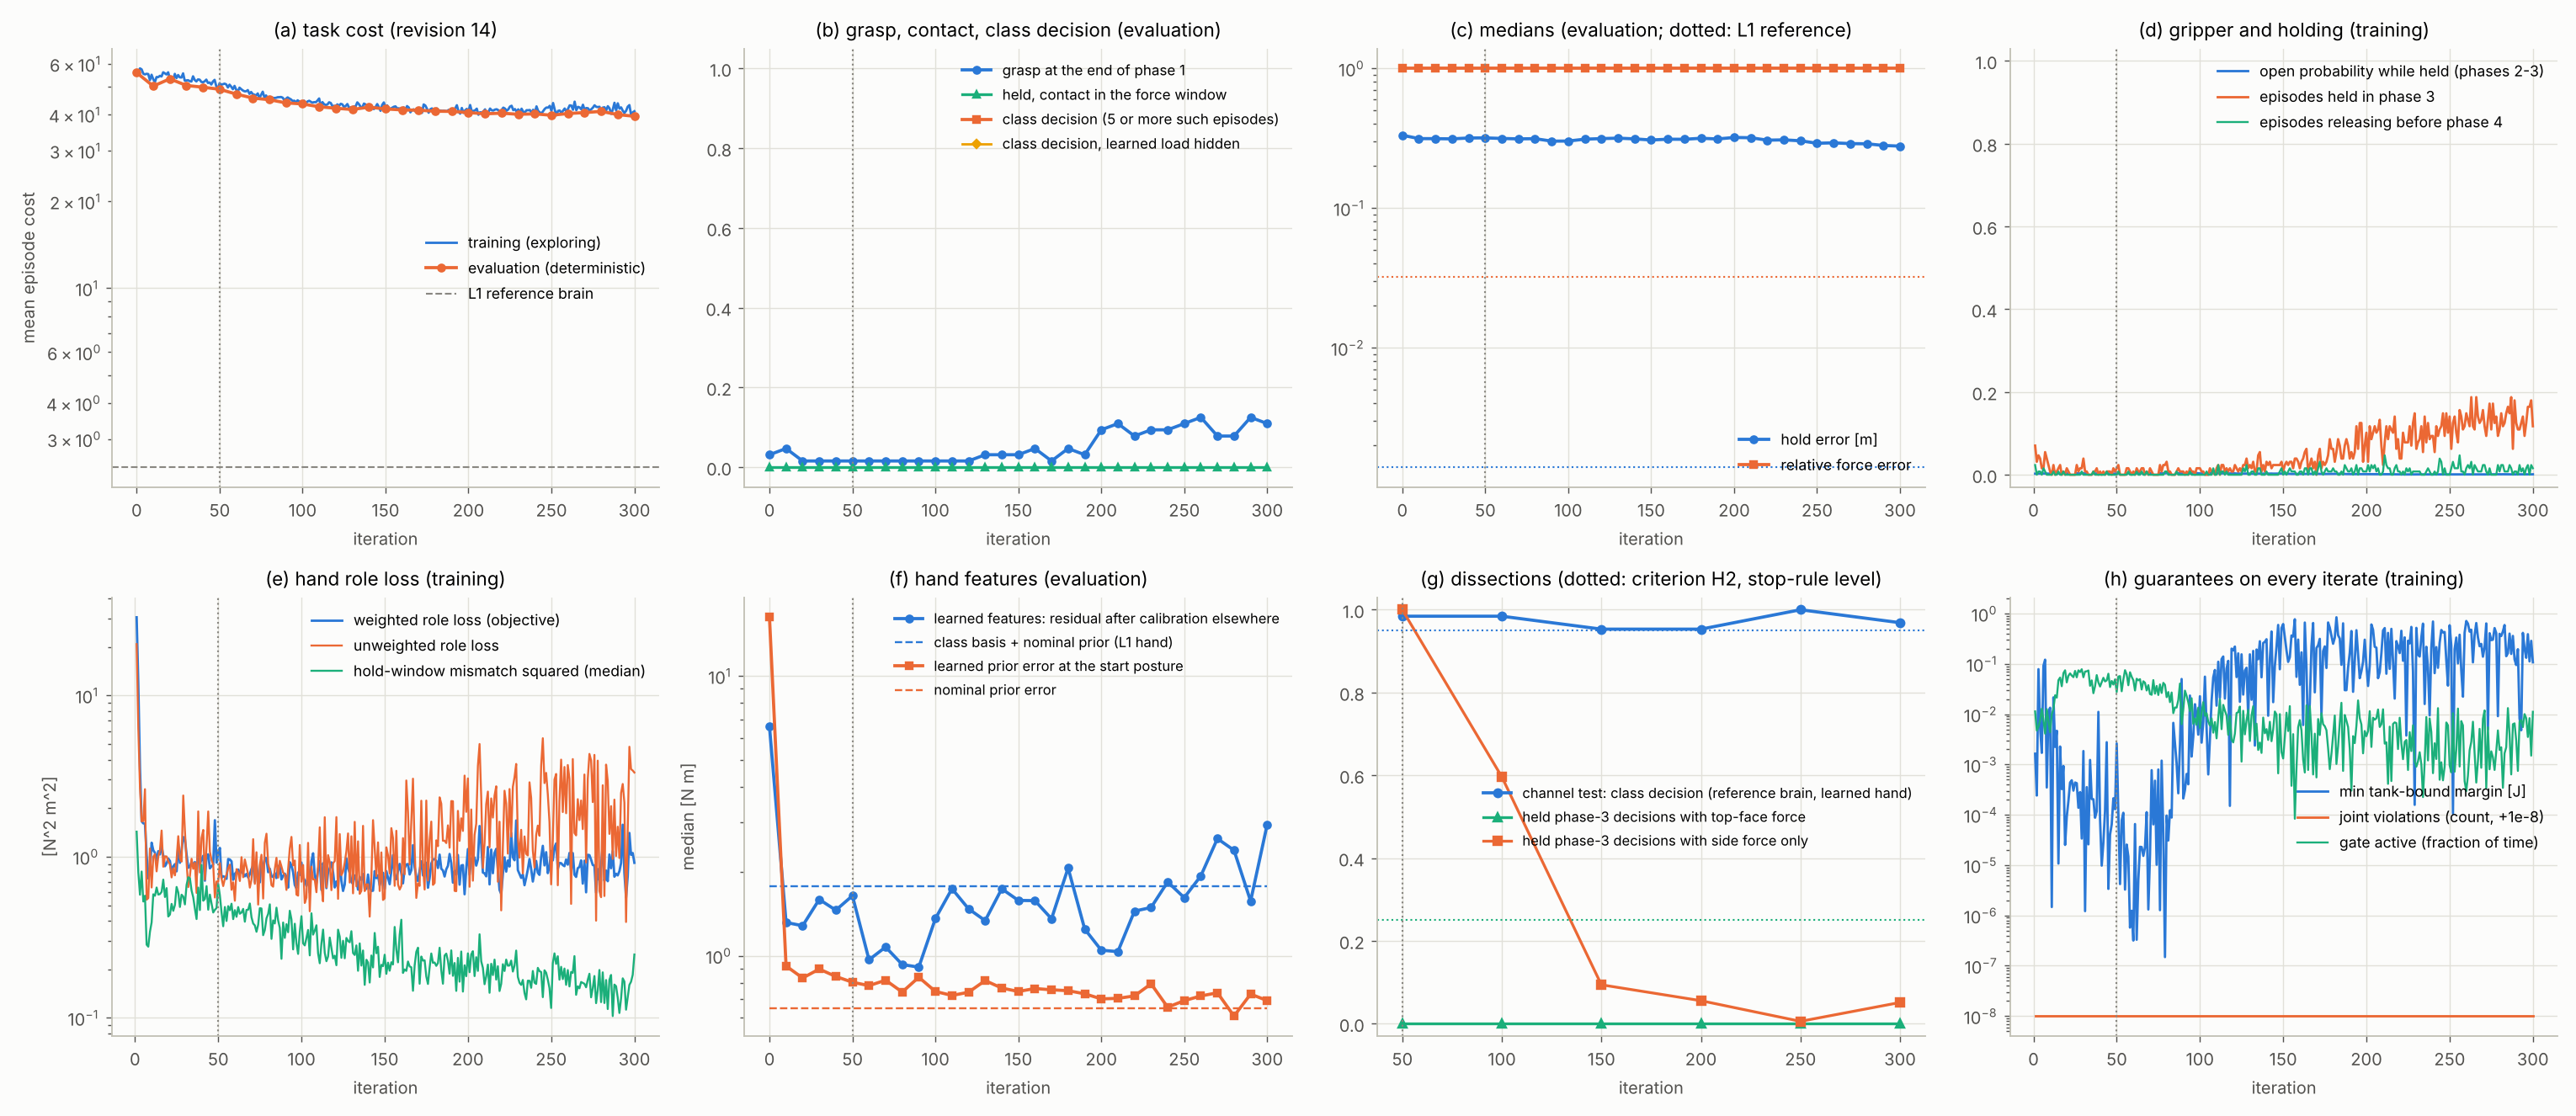
\includegraphics[width=\textwidth]{l2_attempt2.png}
\caption{L2 attempt 2: learning curves and diagnostics}
\label{fig:l2a2}
\end{figure}

\textbf{결과 (반복 300, \Cref{fig:l2a2}).}
\begin{itemize}
\item \textbf{(G) 충족.} 반복 1--50(\texttt{l2\_attempt2b})과 51--300의 300번 모두에서 관절 위반 0, 유한하지 않은 상태 0이고, tank 하한 여유의 최솟값은 $1.5\cdot10^{-7}$ J였다.
\item \textbf{(H2) 충족, (H1) 미충족.} 학습된 손으로 돌린 기준 뇌의 등급 결정은 0.969였다. 다른 자세로 옮긴 오차의 중앙값은 2.947 N\,m로 기준 1.768 N\,m를 넘었다. 반복 60--300의 평가 25번 가운데 6번이 기준을 넘었고(범위 0.910--2.947 N\,m), 마지막 다섯 번 가운데 넷이 넘었다.
\item \textbf{뇌 (기술).} 평가에서 잡기는 0.109, 잡는 점까지 최근접 거리의 중앙값은 0.033 m, 2 cm 안에 든 episode는 29.7\%였다. 단계 2를 든 채 마친 7개 episode에서 단계 2 끝의 goal 손끝은 $p^\star$에서 0.263 m 떨어져 있었다. 단계 3에서 든 10개 episode의 손끝은 윗면보다 0.106 m 아래, $p_c$에서 옆으로 0.186 m에 있었고 윗면 접촉은 없었다. 학습 rollout에서 단계 2와 3의 든 상태로 gripper를 여는 확률은 결정마다 0.0007과 0.0012였고(첫 시도의 반복 100에 0.619와 0.736), 단계 4 전에 놓은 episode는 3.1\%였다.
\item \textbf{Critic.} 단계별 explained variance는 0.936, 0.916, 0.948, 0.649였다.
\item \textbf{중단 규칙.} 물체를 든 채 힘 구간에서 윗면을 누른 평가 episode가 0\%로 25\%에 못 미쳐, 사전 등록대로 run을 멈추고 분해했다.
\end{itemize}

\begin{figure}[H]
\centering
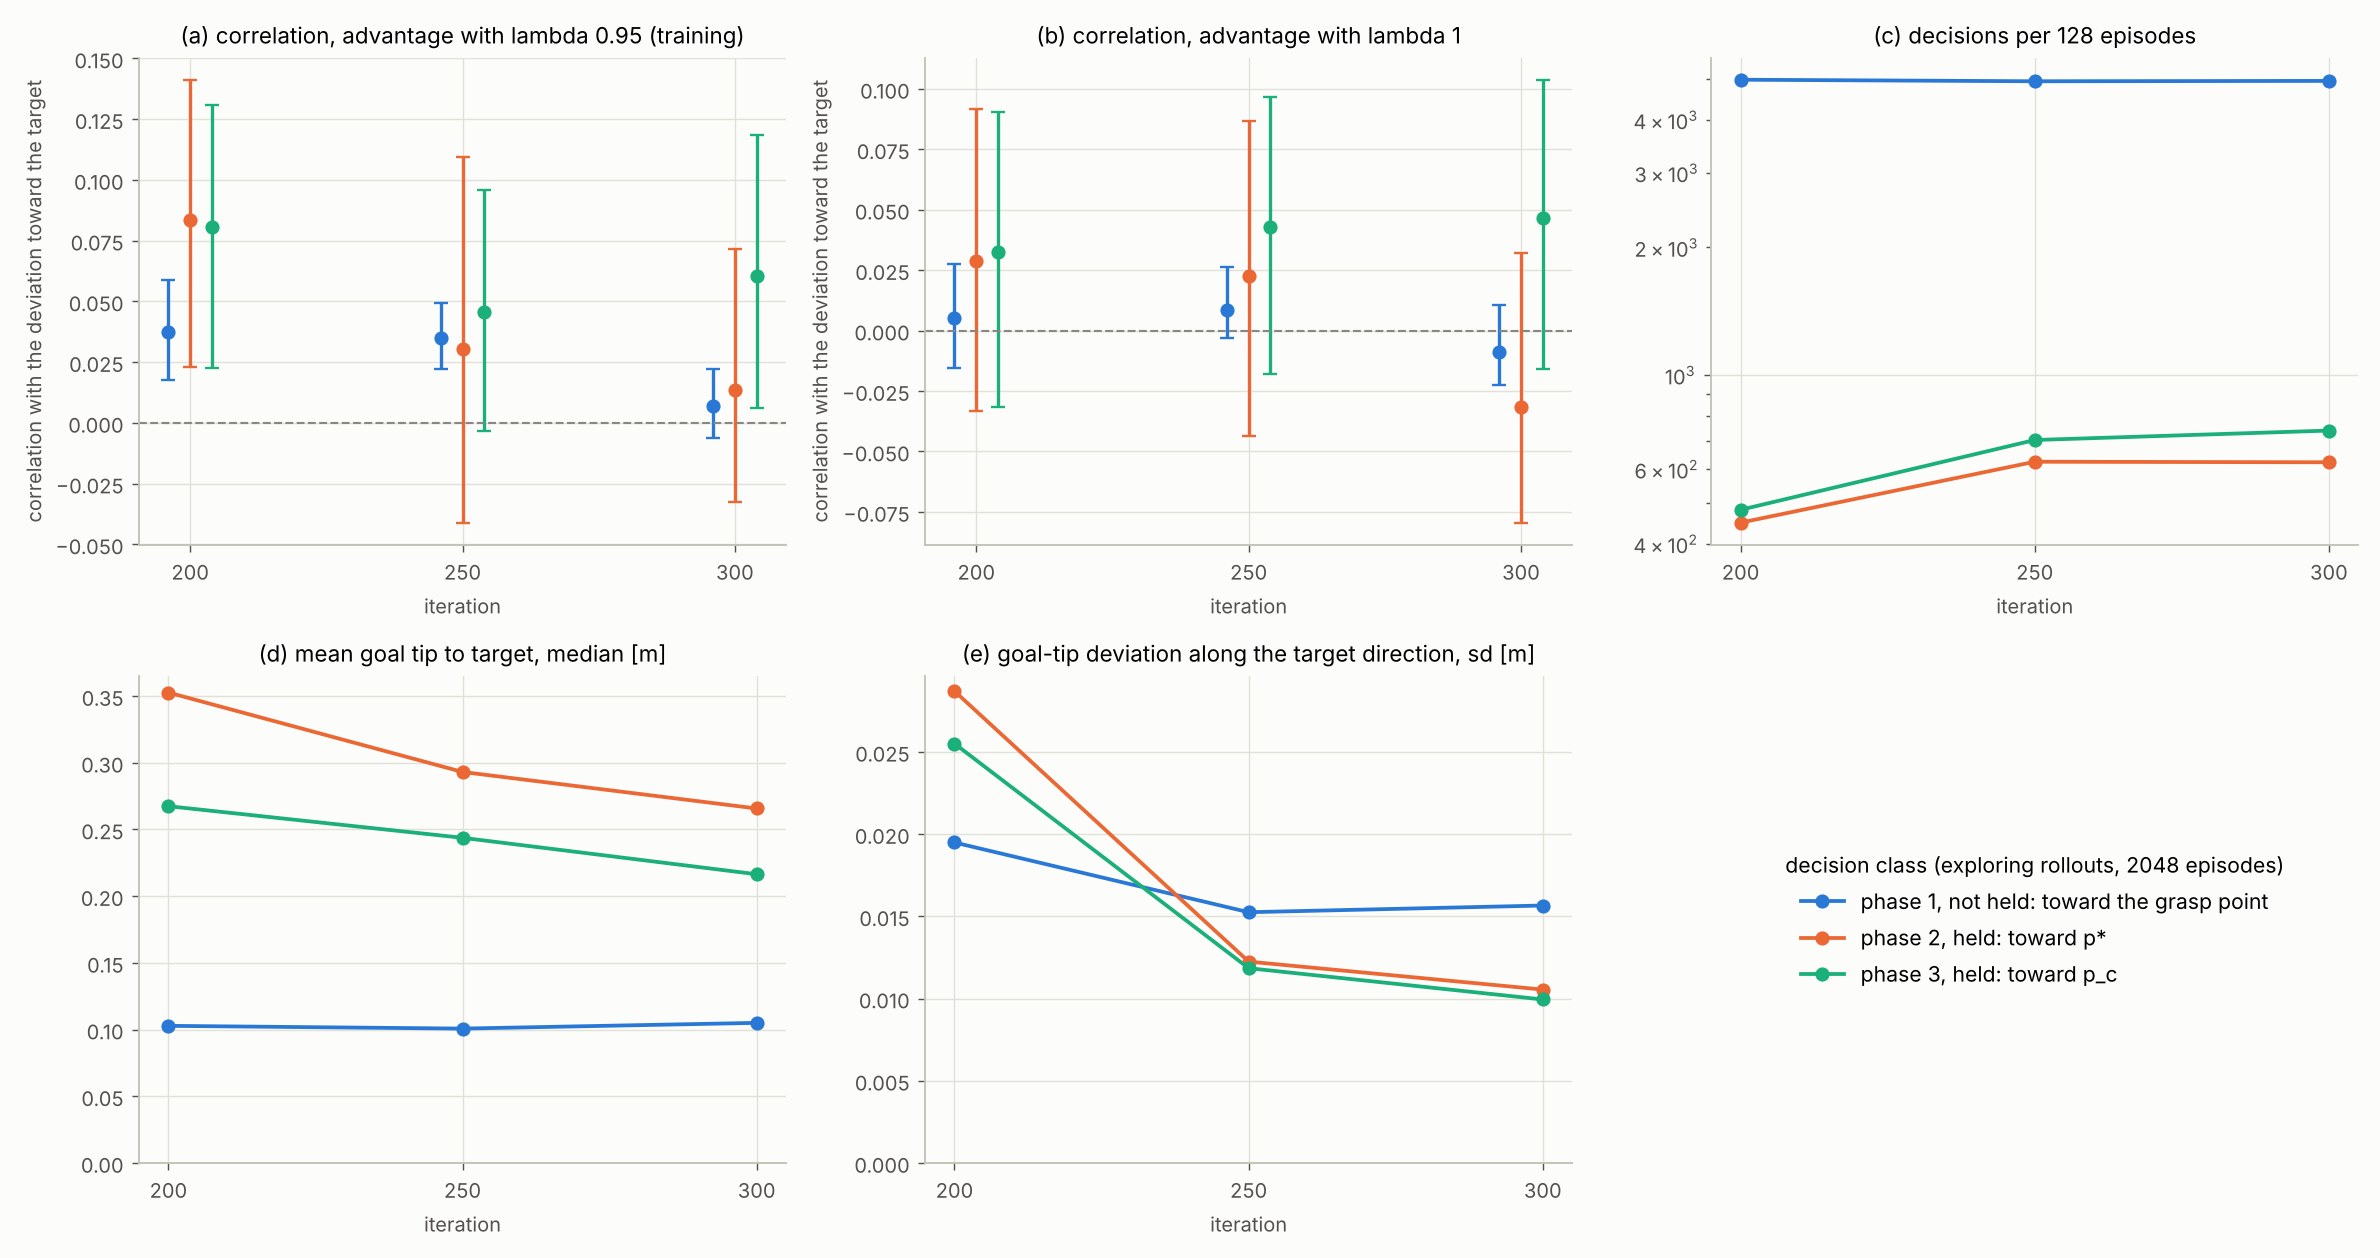
\includegraphics[width=\textwidth]{l2_signal.png}
\caption{Learning signal of the brain by phase}
\label{fig:l2signal}
\end{figure}

\textbf{분해 1: 뒤 단계의 학습 신호 (수정 6과 그 정정, \Cref{fig:l2signal}).} 질문은 단계 2와 3을 배우지 못한 이유가 학습 신호의 방향은 맞지만 든 상태가 잡기 뒤에만 생겨 드물기 때문인지, 신호의 방향이 틀렸기 때문인지이다. 탐색 rollout(pool의 episode 2{,}048개)의 결정을 세 부류로 나눈다: 단계 1에서 물체가 없는 결정(목표는 잡는 점), 단계 2에서 든 결정(목표 $p^\star$), 단계 3에서 든 결정(목표 $p_c$). 표본 행동과 평균 행동의 goal 손끝 차이를 $\delta$, 평균 goal 손끝에서 목표로 가는 단위 벡터를 $e$라 하고, $\delta^\top e$와 GAE advantage $\hat A$의 상관계수를 episode 단위 bootstrap의 95\% 구간과 함께 잰다. 첫 epoch에서 PPO가 평균을 움직이는 방향은 $\mathbb E[\hat A\,\Sigma^{-1}(u-\mu)]$이므로, 상관이 양수이면 표본이 평균 goal을 목표 쪽으로 민다.
\begin{itemize}
\item \textbf{반복 200.} 상관($\lambda=0.95$)은 단계 1, 2, 3에서 0.038 [0.018, 0.059], 0.084 [0.023, 0.141], 0.081 [0.022, 0.131]이었고, 128 episode당 결정 수는 4{,}971, 448, 481이었다. 처음 등록한 episode 256개로는 든 episode가 16개와 17개뿐이어서, 0을 포함하는 구간을 ``틀림''으로 읽는 규칙이 드문 신호를 틀렸다고 판정하게 되어 있었다. 그래서 반복 250과 300을 계산하기 전에 episode를 2{,}048개로 늘리고, 0을 포함하는 구간을 ``미결''로 읽도록 고쳤다.
\item \textbf{반복 300 (판정).} 단계 3은 0.061 [0.006, 0.118]로 맞았고, 단계 2는 0.013 [$-$0.033, 0.071]로 미결이었다. 기준으로 삼은 단계 1도 0.007 [$-$0.006, 0.022]로 떨어졌다. $\lambda=1$의 구간은 세 부류 모두 0을 포함했다. 등록한 판정은 ``맞지만 드물다''가 아니므로, 이 근거로는 조치를 제안하지 않는다.
\item \textbf{기술 (반복 250 뒤에 본 것, 등록 밖).} 든 상태에서 목표 방향 편차의 표준편차는 0.029 m와 0.025 m(반복 200, 단계 2와 3)에서 0.011 m와 0.010 m(300)로 줄었다. 행동의 표준편차 $\sigma_u$의 중앙값은 0.055와 0.058에서 0.038과 0.036으로, goal의 tanh 기울기 $1-\tanh^2\mu$의 중앙값은 0.963과 0.975에서 0.780과 0.879로 줄었다. 정책이 탐색을 줄였고, 단계 2에서는 goal이 관절 범위의 끝 쪽으로 옮겨 tanh의 기울기도 작아졌다.
그동안 평균 goal 손끝은 목표에 다가갔다($p^\star$까지 0.353, 0.293, 0.266 m, $p_c$까지 0.267, 0.244, 0.216 m; 반복 200, 250, 300).
\end{itemize}

\textbf{분해 2: 손의 오차 (수정 7).}
\begin{itemize}
\item \textbf{(a) Optimizer 잡음이 아니다.} 반복 210--300의 checkpoint 열 개의 오차는 1.034--2.947 N\,m(25 백분위 1.507 N\,m)였고, 그 weight를 평균한 손은 1.874 N\,m였다.
\item \textbf{(b) 학습 data 밖의 외삽이다.} 반복 300의 탐색 rollout에서 물체를 든 채 손끝이 $p^\star$에서 0.05 m 안에 있는 결정은 128 episode당 0.06개였다(시작 잡는 점 근처는 114.5개). 오차를 재는 두 자세 가운데 $p^\star$의 자세에서 짐을 든 상태가 role loss에 거의 들어오지 않는다.
\item \textbf{기능은 남았다.} 기준 뇌를 학습된 손으로 돌리면 등급 결정 0.969, 상대 힘 오차 0.0364, 유지 오차 0.0016 m이고, L1의 손으로는 1.000, 0.0311, 0.0016 m이다. 기준 뇌는 $p^\star$에서 정지하므로 rest gate의 기억이 그 자세에서 다시 보정한다.
\end{itemize}

\textbf{해석.} 결합 학습에서 두 구성요소의 data는 모두 뇌의 현재 정책이 처음 상태에서 만든 상태 분포에서 온다. 뇌가 아직 가지 못하는 상태(물체를 든 채 $p^\star$ 근처, 누르기)는 이 분포에 거의 없다. 그래서 손은 그 상태에서 역할을 배우지 못했고(분해 2), 뇌는 뒤 단계를 적은 표본으로 천천히 배웠다. 단계 2와 3의 든 결정은 각각 단계 1 결정의 0.13배와 0.15배였고, 100 반복에 평균 goal 손끝이 $p^\star$ 쪽으로 0.087 m 다가갔다. 뇌에 대한 이 해석은 등록한 판정으로 확인되지 않았다(분해 1). 개정 14의 비용은 놓기 유인을 없앴고, 보장은 학습과 무관하게 모든 반복에서 성립했다. 개정 14가 reaching의 학습을 늦춘 경로는 미해결이다.

\textbf{제안 (추가하지 않음, 승인 대기).} 학습의 시작 상태 분포를
\[
\mu=(1-\beta)\,\mu_0+\tfrac{\beta}{2}\,\mu_2+\tfrac{\beta}{2}\,\mu_3,\qquad \beta=0.5
\]
로 바꾼다. $\mu_0$은 지금의 시작 분포이다. $\mu_2$는 단계 2의 시작에서 잡는 점의 자세 $q_o$에 물체를 든 상태, $\mu_3$은 단계 3의 시작에서 $p^\star$의 자세 $q_s$에 물체를 든 상태이다. 두 자세는 episode 생성기가 이미 계산하는 역기구학 해이고, 속도는 0, 기억은 $z=0$, tank 에너지는 그 episode의 $E_0$, 남은 단계의 길이는 그 episode의 값이다. 비용, network, 보장 장치, 평가(시작 분포 $\mu_0$)는 그대로 둔다. 근거는 셋이다.
\begin{enumerate}[label=(\roman*)]
\item 표 형식의 정책 경사에서 $\varepsilon$-최적에 이르는 반복 수의 상한은 분포 불일치 계수 $\|d^{\pi^\star}_\rho/\mu\|_\infty$의 제곱에 비례한다(Agarwal 등 2021, Definition 3.1, Theorem 4.1). $\mu_0$에서는 $p^\star$ 근처의 든 상태가 지금의 정책 아래 거의 방문되지 않으므로 이 계수가 크다. $\mu_2$와 $\mu_3$은 뇌의 실력과 무관하게 그 상태에 질량을 준다.
\item 같은 $\mu$가 손의 role loss에 $p^\star$ 자세의 짐을 든 상태를 넣는다(분해 2(b)). 하나의 변경이 두 구성요소의 data 범위를 함께 다룬다.
\item 잡아서 쌓는 과제에서 손에 물체를 든 상태나 미리 학습한 제어기의 궤적 위 상태에서 episode를 시작하면 학습이 크게 빨라졌다(Popov 등 2017, Section VII).
\end{enumerate}
이 변경은 든 상태에서 줄어든 탐색과 reaching의 느린 학습은 다루지 않는다. 뇌에 대한 근거가 판정으로 확인되지 않았으므로, 채택 전에 결정 pilot을 사전 등록해 돌리는 것을 제안한다. 반복 300의 checkpoint에서 같은 seed로 두 arm을 50 반복씩 돌린다: A는 그대로, B는 $\mu$로. 읽는 값은 다음과 같다.
\begin{itemize}
\item $\mu_2$와 $\mu_3$에서 시작한 평가의 뒤 단계 기술: 단계 2 끝의 옮기기 오차, 힘 구간에서 윗면을 누른 몫, 힘 오차.
\item $\mu_0$에서 시작한 평가의 reaching이 나빠지지 않는지.
\item 손의 오차: 마지막 다섯 평가의 평균.
\item $p^\star$ 근처에서 든 상태의 범위.
\end{itemize}

\subsection{L2 pilot R: 시작 상태 분포}
\label{sec:l2pr}

\textbf{질문.} 든 상태를 덮는 학습 시작 상태 분포가 첫 단계를 늦추지 않으면서 뇌의 뒤 단계(옮기기, 누르기) 학습을 앞당기고, 손에 $p^\star$ 자세의 짐 든 data를 주는가. \Cref{sec:l2a2}의 제안이며 2026년 11월 15일 사용자가 승인했다.

\textbf{준비에서 드러난 것.}
\begin{itemize}
\item \textbf{Role loss 가중치의 구현 결함.} 코드가 첫 제어 시각의 잡기 상태를 episode 이전의 상태로 썼다. 그래서 첫 결정에서 잡은 episode는 그 잡기가 짐의 변화로 세어지지 않았고, 짐 든 구간 전체가 가중치 1을 받아 prior가 물체의 짐을 떠맡았다. Pool의 6{,}144개 가운데 36개(0.59\%)가 손끝이 잡는 점에서 2 cm 안에서 시작해 첫 결정에서 잡힌다. Episode 이전을 놓은 상태로 두어 \Cref{def:coupled}의 $r(t)$와 맞췄다. 그런 episode가 없는 batch의 손실은 끝자리까지 같고, 있는 batch의 가중 손실은 1.842에서 0.761로, 1.481에서 0.903으로 바뀌었다. 두 번째 시도의 손은 이 결함 아래에서 학습했으므로, (H1)의 미충족에서 이 결함의 몫은 분해 2의 판정과 갈리지 않는다.
\item \textbf{Critic warm-up.} 시작 분포를 바꾸면 critic은 새 상태의 가치를 모른다. 처음 등록한 B를 2 반복 돌린 smoke test에서 첫 PPO update의 KL은 4.12, clip 비율은 0.720, value loss는 87.0이었다(두 번째 시도의 재개 직후 0.133, 0.425, 1.41). 그래서 처음 5 반복은 actor와 손을 고정하고 critic만 학습한다. 개선 전에 평가부터 맞추는 것이다. 단계-3 restart에서 critic의 explained variance는 0.468에서 0.698로 올랐고, 그 뒤 첫 두 update의 KL은 0.767과 0.190이었다.
\item \textbf{개정 14의 과힘 놓기 유인.} 아래 사실이다. 반복 300의 checkpoint를 단계-3 restart(256 episode, 탐색)에서 돌리면, 든 단계-3 결정의 0.339(11{,}927개 가운데 4{,}039개)가 놓는 편이 싼 영역에 있었다. 접촉 힘은 중앙값 $4.24f^\star$, 90 백분위 $9.72f^\star$였다. 그 영역에서 gripper를 여는 확률은 0.0033(다른 곳 0.0021)으로 아직 이용되지 않았지만, 탐색으로 episode의 13\%가 단계 3에서 놓았고 놓는 순간 비용이 내려간다.
\end{itemize}

\begin{fact}[Release incentive under overpressing, revision 14]
\label{fact:release14}
Under the cost of revision 14, $\Pi(o,f)=((f-f^\star)/f^\star)^2$ for $f>0$. Let $t\in\mathcal I_3$ with $f_n(t)>0$, and let $\Omega^1_{\mathrm{task}}$ and $\Omega^0_{\mathrm{task}}$ be the rates with the object held and released at the same configuration ($o=p$). Then $\Omega^0_{\mathrm{task}}-\Omega^1_{\mathrm{task}}=2+\|p-p_c\|/0.1-((f_n-f^\star)/f^\star)^2$, which is negative if and only if $((f_n-f^\star)/f^\star)^2>2+\|p-p_c\|/0.1$; at $p=p_c$, if and only if $f_n>(1+\sqrt2)f^\star$.
\end{fact}

\begin{proof}
\Cref{prop:costprog}(a)의 증명에서 상한 없는 $\Pi$를 쓴다.
\[
\Omega^0_{\mathrm{task}}-\Omega^1_{\mathrm{task}}=\Big(2+\frac{\|p-p_c\|}{0.1}+\frac{|p_x-p^\star_x|}{0.1}\Big)-\Big(\Big(\frac{f_n-f^\star}{f^\star}\Big)^2+\frac{|p_x-p^\star_x|}{0.1}\Big)
\]
$p=p_c$이면 음수 조건은 $|f_n-f^\star|>\sqrt2\,f^\star$이고, $f_n>0$이므로 $f_n>(1+\sqrt2)f^\star$이다.
\end{proof}

\textbf{결정 (개정 15, 2026년 11월 15일 사용자 승인).} 누르기 항에 상한 1을 두었다(\Cref{def:stageBtask}). \Cref{prop:costprog}(a)가 모든 힘으로 넓어지고 (c)가 더해진다. 무작위 자세에서 윗면 force가 있는 상태 가운데 놓는 편이 싼 몫은 개정 14에서 0.885, 개정 15에서 0이다(\texttt{records/cost\_audit.json}). 환경 검증은 V11을 맞추고 V18을 더해 일곱 번째로 돌렸다(\Cref{sec:envcheck}). L1은 개정 15로 다시 돌렸다(\Cref{sec:l1}).

\textbf{구성 (사전 등록, \texttt{records/l2\_pilotR\_plan.md}).}
\begin{itemize}
\item 두 arm 모두 두 번째 시도의 반복 300에서 같은 seed로 55 반복을 돈다. 반복 301--305는 critic warm-up, 306--355가 학습이다. 비용은 개정 15이다.
\item A는 시작 분포를 그대로 둔다. B는 $\mu=0.5\,\mu_0+0.25\,\mu_2+0.25\,\mu_3$를 쓴다(\Cref{sec:l2a2}).
\item 평가는 $\mu_0$, $\mu_2$, $\mu_3$의 세 시작에서 같은 64 episode로 한다. 반복 300의 기준값은 다음과 같다. $\mu_3$에서 정확히 누른 episode(힘 구간의 상대 힘 오차 0.5 미만, 단계 4 시작까지 든 채)는 0개이고, 윗면을 누른 episode는 0.4375, 그 상대 힘 오차의 중앙값은 1.291이다. $\mu_2$에서는 64개 모두 단계 3까지 들었고, 단계 2 끝의 유지 오차의 중앙값은 0.249 m이다.
\item 판정은 반복 355에서 한다. (P) $\mu_3$에서 정확히 누른 몫이 B에서 A보다 0.25 이상 크고, (G0) B의 잡기가 A보다 0.05 넘게 낮지 않으며 최근접 거리의 중앙값이 A보다 0.01 m 넘게 크지 않으면 시작 상태 분포를 세 번째 시도에 쓴다.
\end{itemize}

\begin{figure}[H]
\centering
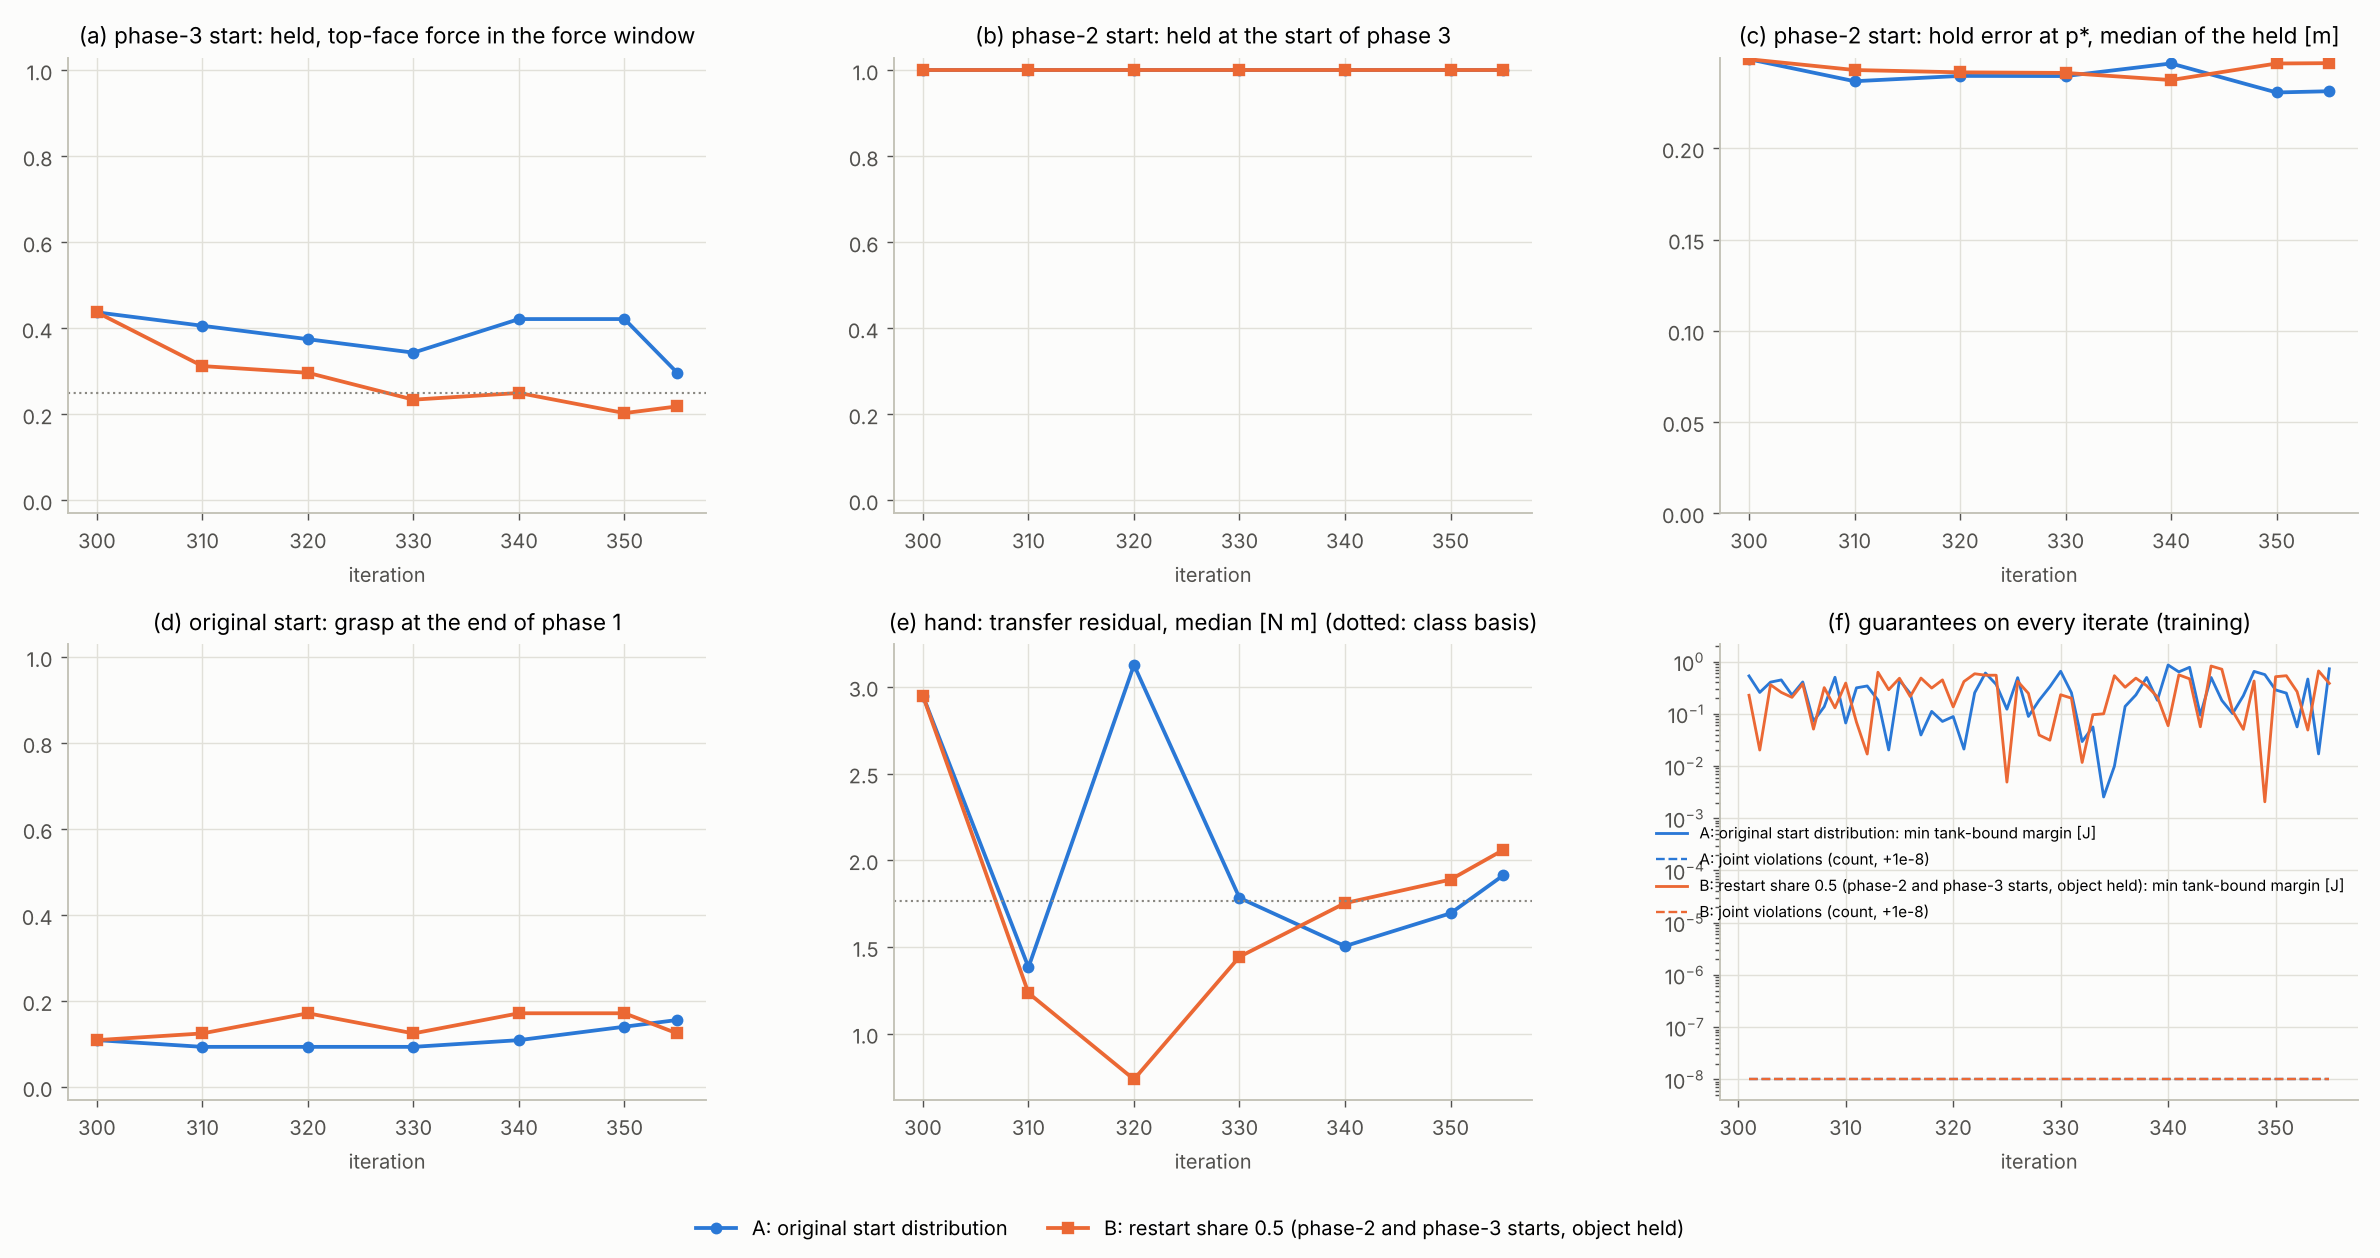
\includegraphics[width=\textwidth]{l2_pilotR.png}
\caption{Pilot R: restart start-state distribution against plain continuation}
\label{fig:l2pr}
\end{figure}

\textbf{결과 (반복 355, \Cref{fig:l2pr}).}
\begin{itemize}
\item \textbf{(P) 실패, 채택하지 않음.} $\mu_3$에서 정확히 누른 몫은 A 0.016(64개 가운데 1개), B 0이었다. (G0)는 성립했다. 잡기는 B 0.125, A 0.156이고, 최근접 거리의 중앙값은 B 0.0345 m, A 0.0313 m였다.
\item \textbf{뒤 단계.} $\mu_3$에서 윗면을 누른 몫은 0.438에서 A 0.297, B 0.219로 줄었고, 그 상대 힘 오차의 중앙값은 1.291에서 A 1.465, B 2.116이 되었다. $\mu_2$에서는 두 arm 모두 64개가 단계 3까지 들었고, 단계 2 끝의 유지 오차의 중앙값은 A 0.231 m, B 0.247 m였다(반복 300에 0.249 m).
\item \textbf{손.} 평가 여섯 번(반복 310--355)의 다른 자세로 옮긴 오차의 평균은 A 1.901 N\,m, B 1.520 N\,m였다. B가 낮지만 여섯 값의 범위가 0.738--3.126 N\,m로 넓다.
\item \textbf{보장.} 두 arm 모두 55 반복에서 관절 위반 0, 유한하지 않은 상태 0이고, tank 하한 여유의 최솟값은 A $2.6\cdot10^{-3}$ J, B $2.1\cdot10^{-3}$ J였다.
\end{itemize}

\textbf{분해 (결과를 본 뒤 더한 기술, 등록 밖).}
\begin{itemize}
\item \textbf{$\mu_3$에서의 행동 (결정적 정책).} 힘 구간에서 든 채 닿지 않은 episode는 36개(반복 300), 45개(A), 50개(B)였다. 그 손끝은 윗면보다 약 0.06 m 아래, $p_c$에서 옆으로 약 0.15 m, 즉 $p_c$ 위가 아니라 block 옆에 있었다. 닿은 경우의 힘은 중앙값 약 $3.5f^\star$였다. Goal 손끝의 높이를 $f/f^\star$에 회귀한 기울기는 $-0.004$, $-0.008$, $-0.014$로 양수가 아니어서, 힘에 따른 되먹임이 없다.
\item \textbf{놓기 (탐색 정책, 256 episode).} $\mu_3$에서 단계 3 안에 놓은 episode는 0.133(반복 300), 0.227(A), 0.445(B)였고, 든 단계-3 상태에서 여는 확률은 0.0025, 0.0048, 0.0130이었다. 반복 355의 두 arm에서 놓는 순간의 힘의 중앙값은 0이어서, 대부분의 놓기는 과힘의 순간에 일어나지 않았다.
\item \textbf{학습 신호 ($\mu_2$, $\mu_3$에서 시작, 512 episode).} 든 결정이 128 episode당 4{,}500--6{,}200개로 많아도, advantage와 목표 방향 goal 편차의 상관은 단계 2($p^\star$ 방향)에서 $-0.035$ $[-0.075,\ 0.008]$(반복 300), $-0.013$ $[-0.064,\ 0.034]$(A), $0.013$ $[-0.029,\ 0.054]$(B), 단계 3($p_c$ 방향)에서 $-0.008$ $[-0.041,\ 0.022]$, $-0.030$ $[-0.070,\ 0.009]$, $-0.003$ $[-0.039,\ 0.032]$였다. 목표 방향 편차의 표준편차는 0.012--0.016 m였다. 두 번째 시도의 반복 200에는 이 편차가 0.025--0.029 m였고 상관이 0.08로 양수였다(분해 1).
\end{itemize}

\textbf{해석.} 시작 상태 분포는 든 상태의 표본을 충분히 주었지만, 그 표본에 목표 쪽으로 가라는 신호가 없었다. 목표 방향 탐색이 1.2--1.6 cm로 줄어, 한 표본이 비용에 주는 차이가 advantage의 잡음에 묻힌다. 대신 B가 배운 것은 자기의 과힘 아래에서 단계 3을 든 채 보내지 않는 것, 즉 닿지 않거나 놓는 것이었다. 단계 1에도 같은 정밀도의 문제가 있다. 2 cm 안에 든 episode는 A 0.328, B 0.375인데 가장 가까운 순간에 잡을 만큼 느린 episode는 0.078, 0.109이고, 두 번째 시도의 반복 300에 결정적 goal 손끝은 잡는 점에서 0.089 m 떨어져 있었다. 세 단계 모두에서 뇌는 task 공간의 정밀한 목표(2 cm 안에서 멈추기, 0.25 m 옮기기, 몇 mm의 깊이로 힘 맞추기)와 그 방향의 탐색을 내야 하는데, 지금의 행동은 관절 상자 안의 절대 자세이다. 그래서 목표마다 역기구학을 배워야 하고, 탐색의 크기는 관절 공간의 표준편차로 간접적으로 정해진다. L1의 기준 뇌는 공칭 Jacobian으로 task 공간의 수정을 관절 목표에 더하는 구조로 과제를 풀었다(\Cref{sec:l1}).

\textbf{제안 (추가하지 않음, 승인 대기).} 뇌의 행동을 class 수준의 기구학을 쓰는 task 공간의 변위로 바꾼다.
\[
q_d=\Pi_{\mathcal B}\big(q+J_{\mathrm{nom}}(q)^{+}\,\Delta p\big),\qquad \Delta p=\delta_{\max}\tanh(u_{1:2})\in\R^2
\]
$\Pi_{\mathcal B}$는 관절 상자로의 사영, $J_{\mathrm{nom}}$은 공칭 길이의 Jacobian이고, 강성과 gripper는 그대로이다. 근거는 셋이다. (i) 공칭 기구학은 손의 공칭 prior와 같은 class 수준의 구조이며 instance 모형이 아니다. (ii) 정밀도와 탐색이 과제의 단위(m)로 정해지고, 관측에 이미 있는 상대 위치($o-p$, $p^\star-p$)에서 필요한 사상이 거의 항등이 된다. 힘은 $\Delta p_y$와 강성으로 직접 정해진다. (iii) Goal이 상자 안에 머무르므로 보장 장치(제약층, tank, guard)는 바뀌지 않는다. 채택 전에, 초기화에서 같은 seed로 두 arm(지금의 행동 대 task 공간의 행동, 둘 다 개정 15와 시작 상태 분포)을 돌려 뒤 단계의 학습 신호와 기술을 비교하는 결정 실험을 사전 등록해 돌리는 것을 제안한다.

\subsection{L2 pilot T: task 공간의 행동}
\label{sec:l2pt}

\textbf{질문.} Class 수준의 기구학을 쓰는 task 공간의 행동이, 같은 조건의 관절 공간 절대 자세에 비해 뇌에 뒤 단계(옮기기, 누르기)의 학습 신호와 기술, 그리고 정밀한 reaching을 주는가. \Cref{sec:l2pr}의 제안이며 2026년 11월 15일 사용자가 승인했다.

\textbf{행동 (\texttt{src/pairl/learn/l2.py}의 goal\_of).}
\[
q_d=\Pi_{\mathcal B}\big(q+J_{\mathrm{nom}}(q)^{+}\Delta p+n\,v_N\big),\qquad \Delta p=0.3\tanh(u_{1:2})\ \mathrm{m},\qquad n=0.3\tanh(u_3)\ \mathrm{rad}
\]
$J_{\mathrm{nom}}^{+}=J_{\mathrm{nom}}^\top(J_{\mathrm{nom}}J_{\mathrm{nom}}^\top+0.02^2I)^{-1}$이고 $v_N$은 $J_{\mathrm{nom}}$의 kernel의 단위 방향, $q$는 측정 자세이다. 강성, gripper, 관측, network는 두 방식에서 같다. 행동 0은 $q_d=q$를 준다. $\|\Delta p\|\le0.05$ m이면 공칭 손끝은 $\Delta p$만큼 움직이고 그 오차의 중앙값은 1.4 mm(95 백분위 4.8 mm)이다. Null 방향의 0.1 rad는 손끝을 0.5 mm 움직인다. 초기화에서 restart를 섞어 돌린 rollout은 관절 위반 0이었다. 처음 탐색은 task 공간에서 맞췄다. 관절 방식(처음 goal 표준편차 0.1)은 축마다 0.067 m, task 방식(0.22)은 0.063 m이다.

\textbf{구성 (사전 등록, \texttt{records/l2\_pilotT\_plan.md}).} 두 arm 모두 초기화에서 같은 seed로 100 반복을 돈다. 비용은 개정 15, role loss는 가중치를 쓰고, 시작 상태 분포는 \Cref{sec:l2pr}의 B와 같다. 판정은 반복 100에서 한다. (G) T의 잡기가 J보다 0.05 넘게 낮지 않고, (P1) $\mu_3$에서 정확히 누른 몫이 T에서 J보다 0.25 이상 크거나 (P2) $\mu_2$에서 T의 유지 오차가 J의 절반 이하이고 든 몫이 0.1 넘게 낮지 않으면, task 공간의 행동을 채택한다(개정 16).


\begin{figure}[H]
\centering
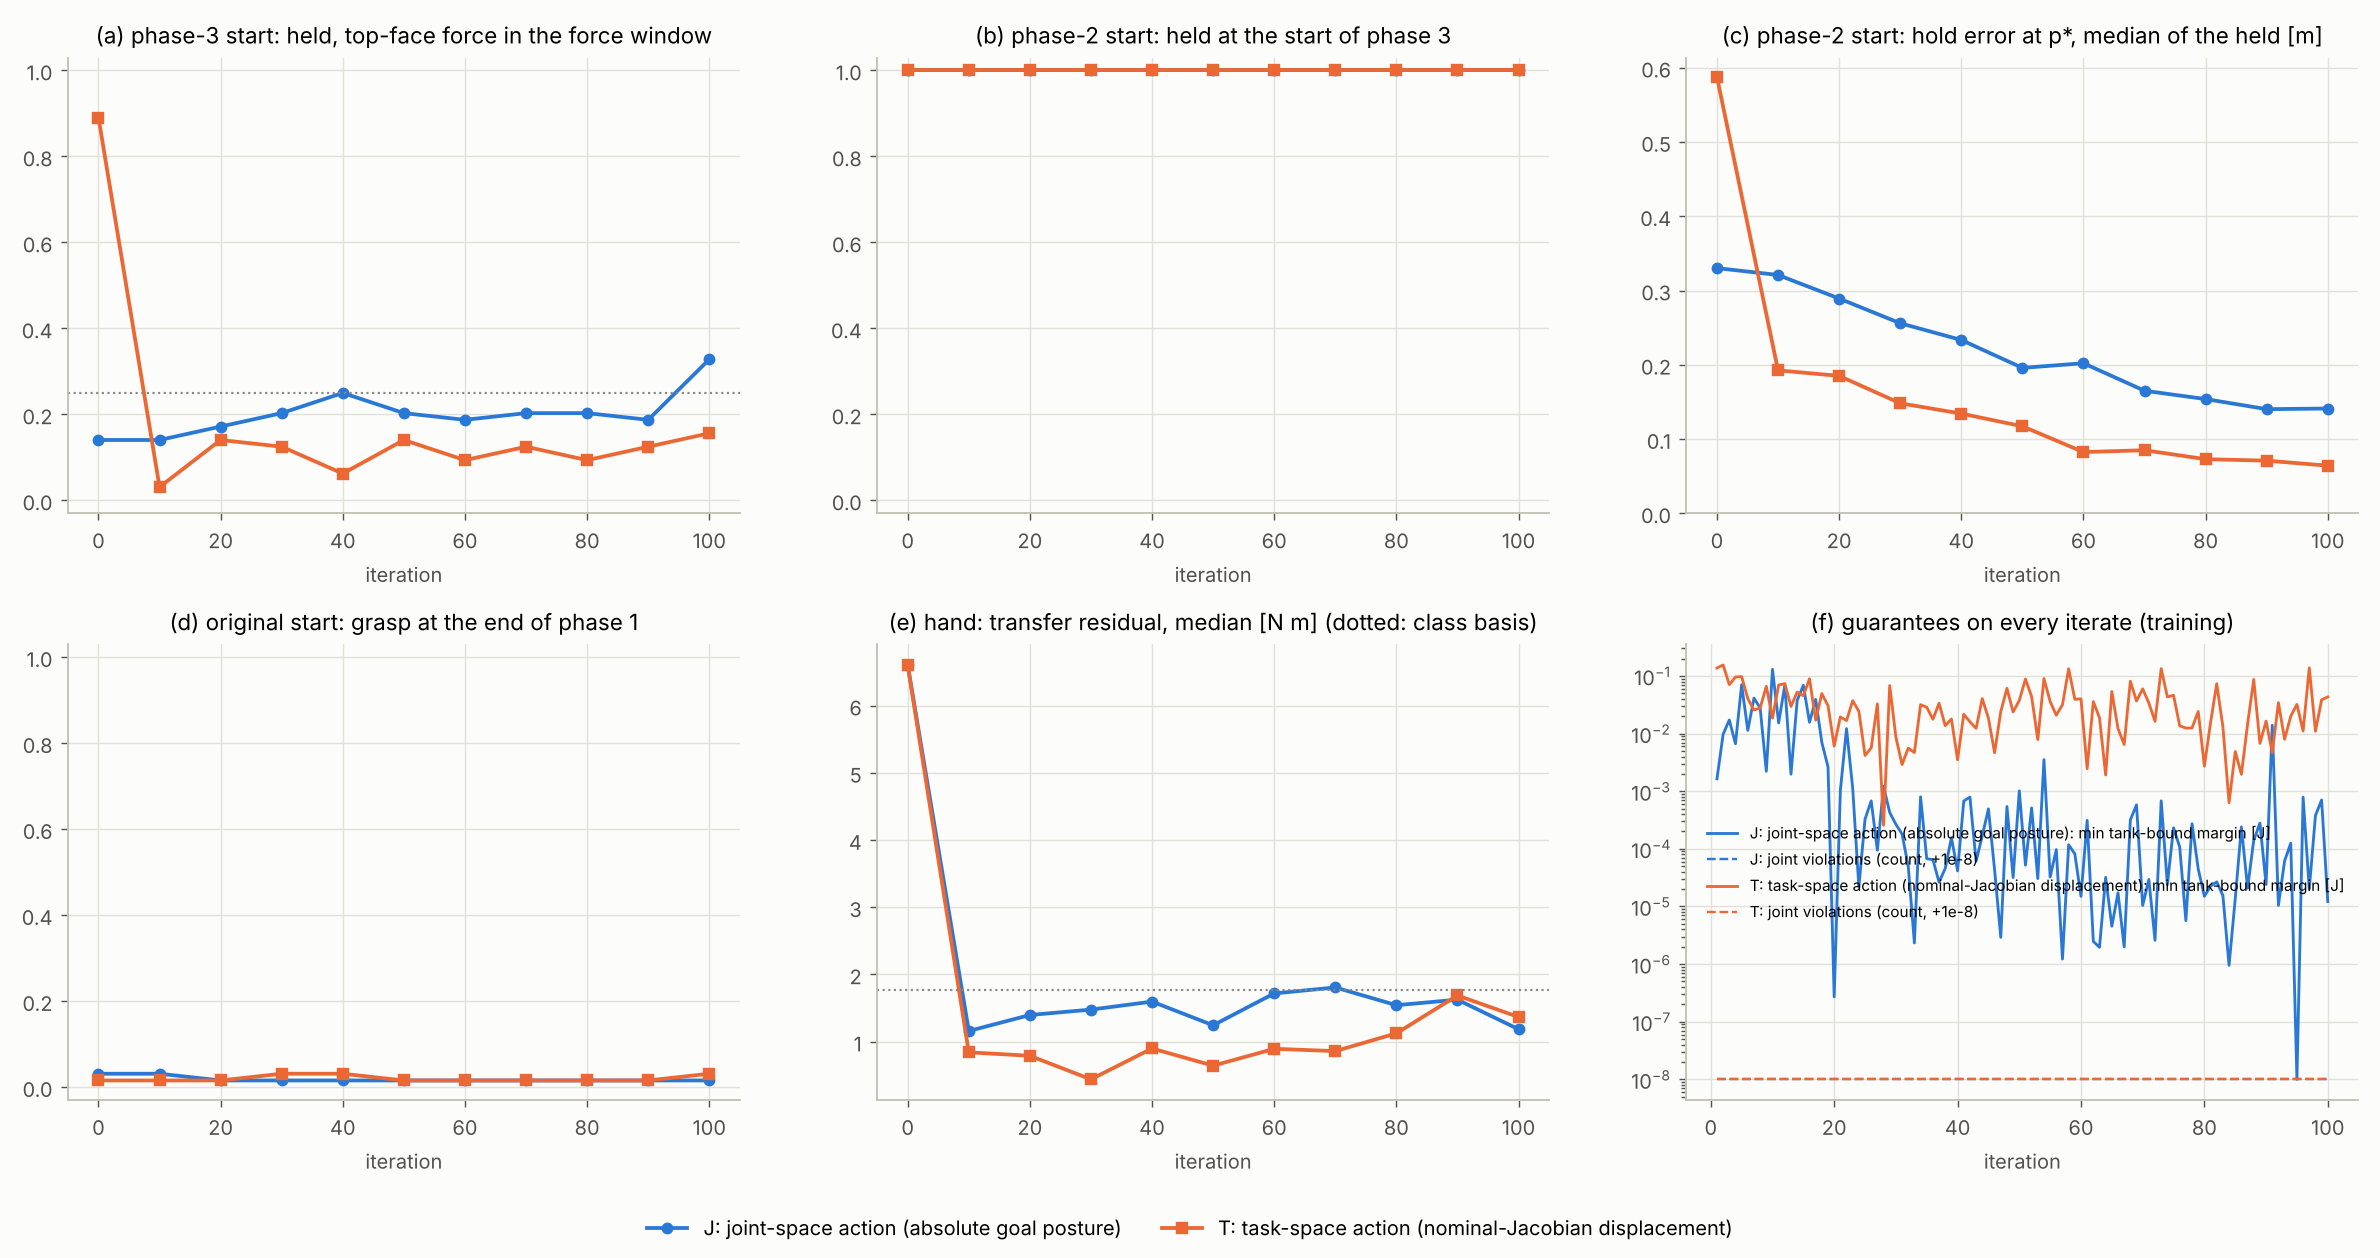
\includegraphics[width=\textwidth]{l2_pilotT.png}
\caption{Pilot T: task-space action against joint-space action}
\label{fig:l2pt}
\end{figure}

\textbf{결과 (반복 100, \Cref{fig:l2pt}).}
\begin{itemize}
\item \textbf{(P2) 성립, 채택(개정 16).} $\mu_2$에서 $p^\star$의 유지 오차는 T 0.0642 m로 J의 절반(0.0706 m) 아래였고, 두 arm 모두 64개가 단계 3까지 들었다. T의 오차는 반복 10부터 모든 평가에서 J보다 작았다(반복 100에 T 0.064 m, J 0.141 m). (G)도 성립했다(잡기 T 0.031, J 0.016). (P1)은 성립하지 않았다($\mu_3$에서 정확히 누른 몫 T 0.078, J 0.094).
\item \textbf{Reaching.} 단계 1의 최근접 거리의 중앙값은 T 0.0172 m, J 0.0868 m이고, 2 cm 안에 든 episode는 64개 가운데 T 35개, J 4개였다. 단계 1 끝의 goal 손끝은 잡는 점에서 T 0.067 m, J 0.172 m였다. 그러나 가장 가까운 순간에 잡을 만큼 느린 episode는 T 0.016, J 0.078이었다.
\item \textbf{학습 신호 ($\mu_2$, $\mu_3$에서 시작, 512 episode).} 단계 2($p^\star$ 방향)에서 T $0.096$ $[0.029,\ 0.149]$, J $0.021$ $[-0.016,\ 0.055]$이고, 단계 3($p_c$ 방향)에서 T $0.004$ $[-0.035,\ 0.046]$, J $0.038$ $[0.007,\ 0.074]$였다. 목표 방향 편차의 표준편차는 단계 2에서 T 0.0082 m, J 0.0145 m, 단계 3에서 T 0.0060 m, J 0.0155 m였다.
\item \textbf{손.} 평가 10--100의 다른 자세로 옮긴 오차의 평균은 T 0.954 N\,m, J 1.475 N\,m이고, 기준 뇌의 등급 결정은 T 0.969, J 0.891이었다.
\item \textbf{보장.} 두 arm 모두 100 반복에서 관절 위반 0, 유한하지 않은 상태 0이고, tank 하한 여유의 최솟값은 J $2.7\cdot10^{-9}$ J, T $2.6\cdot10^{-4}$ J였다.
\item \textbf{$\mu_3$에서의 행동 (기술).} T는 64개 가운데 54개에서 물체를 $p_c$ 위(옆으로 0.014 m, 윗면 위 0.069 m)에 든 채 누르지 않았고, 닿은 경우의 힘은 중앙값 $0.80f^\star$였다. J는 21개에서 닿았고(힘 중앙값 $1.28f^\star$), 43개는 윗면 위 0.029 m, 옆으로 0.081 m에 떠 있었다.
\end{itemize}

\textbf{해석.} Task 공간의 행동은 ``어디로''의 문제를 풀었다. 잡는 점에 손끝을 가져가는 정밀도(2 cm 안이 64개 가운데 4개에서 35개)와 $p^\star$로 옮기기가 좋아졌고, 옮기기에는 0이 아닌 학습 신호가 생겼다. 탐색 폭은 J보다 작았으므로(0.0082 대 0.0145 m), 이 신호는 탐색을 키워서 생긴 것이 아니다. 남은 문제는 ``어떻게''이다. 잡는 점에 닿아도 잡을 만큼 느리게 멈추지 못하고(0.016), $p^\star$ 위에서 내려가 누르지 않는다(단계 3의 목표 방향 탐색 0.6 cm). 둘 다 도착과 접촉의 속도와 힘이라는 과도 구간의 기술이다. 반복 100은 초기화에서의 예산으로 짧다(두 번째 시도는 반복 200이 넘어서야 잡기가 0.1에 이르렀다).

\textbf{제안 (승인 대기).} 채택한 구성(개정 15, 16, 시작 상태 분포 0.5)을 그대로 쓴 T의 run을 반복 300까지 이어 세 번째 시도로 삼는다. 같은 구성을 초기화에서 다시 돌리지 않으므로 반복 100만큼 아낀다. 사전 등록할 기준은 두 번째 시도의 (G), (H2), 중단 규칙에, (H1)을 마지막 다섯 평가의 평균으로 바꾼 것(\Cref{sec:l2a2}에서 한 평가의 값이 흔들렸다)과 $\mu_2$, $\mu_3$의 기술과 학습 신호를 더한다.

\subsection{L2 세 번째 시도: 채택한 구성으로 반복 300까지}
\label{sec:l2a3}

\textbf{구성 (사전 등록, \texttt{records/l2\_attempt3\_plan.md}).} 개정 15의 비용, 개정 16의 task 공간의 행동, 정정한 role loss의 가중치, 시작 상태 분포 0.5를 쓴다. 이것은 pilot T의 T와 같은 구성이므로, 반복 1--100은 T이고 101--300은 T의 반복 100 checkpoint에서 이어 돈다(2026년 11월 15일 사용자 승인). 이어 도는 시점에 optimizer 상태는 새로 시작한다(pilot T의 checkpoint에는 없다). 이 run부터는 checkpoint에 optimizer 상태도 저장한다.

\textbf{기준 (반복 300).}
\begin{itemize}
\item (G) 반복 1--300의 모든 iterate에서 (C1).
\item (H1) 손: 평가 260--300(다섯 번)의 다른 자세로 옮긴 오차의 중앙값의 평균이 1.768 N\,m 아래. 두 번째 시도에서 한 평가의 값이 두 배까지 흔들렸으므로 평균으로 바꿨다.
\item (H2) 손: 반복 300의 분해에서 기준 뇌를 학습된 손으로 돌린 등급 결정이 0.95 이상.
\item 뇌(기술): $\mu_0$의 잡기, 최근접 거리, 2 cm 안의 몫, 가장 가까운 순간에 잡을 만큼 느린 몫; $\mu_2$의 유지 오차; $\mu_3$의 정확히 누른 몫, 누른 몫, 힘의 비. 학습 신호는 반복 200과 300에서 잰다.
\item 중단 규칙: 반복 300에 $\mu_0$의 평가 episode 가운데 든 채 힘 구간에서 윗면을 누른 것이 25\% 미만이면 run을 멈추고 분해한다.
\end{itemize}

\begin{figure}[H]
\centering
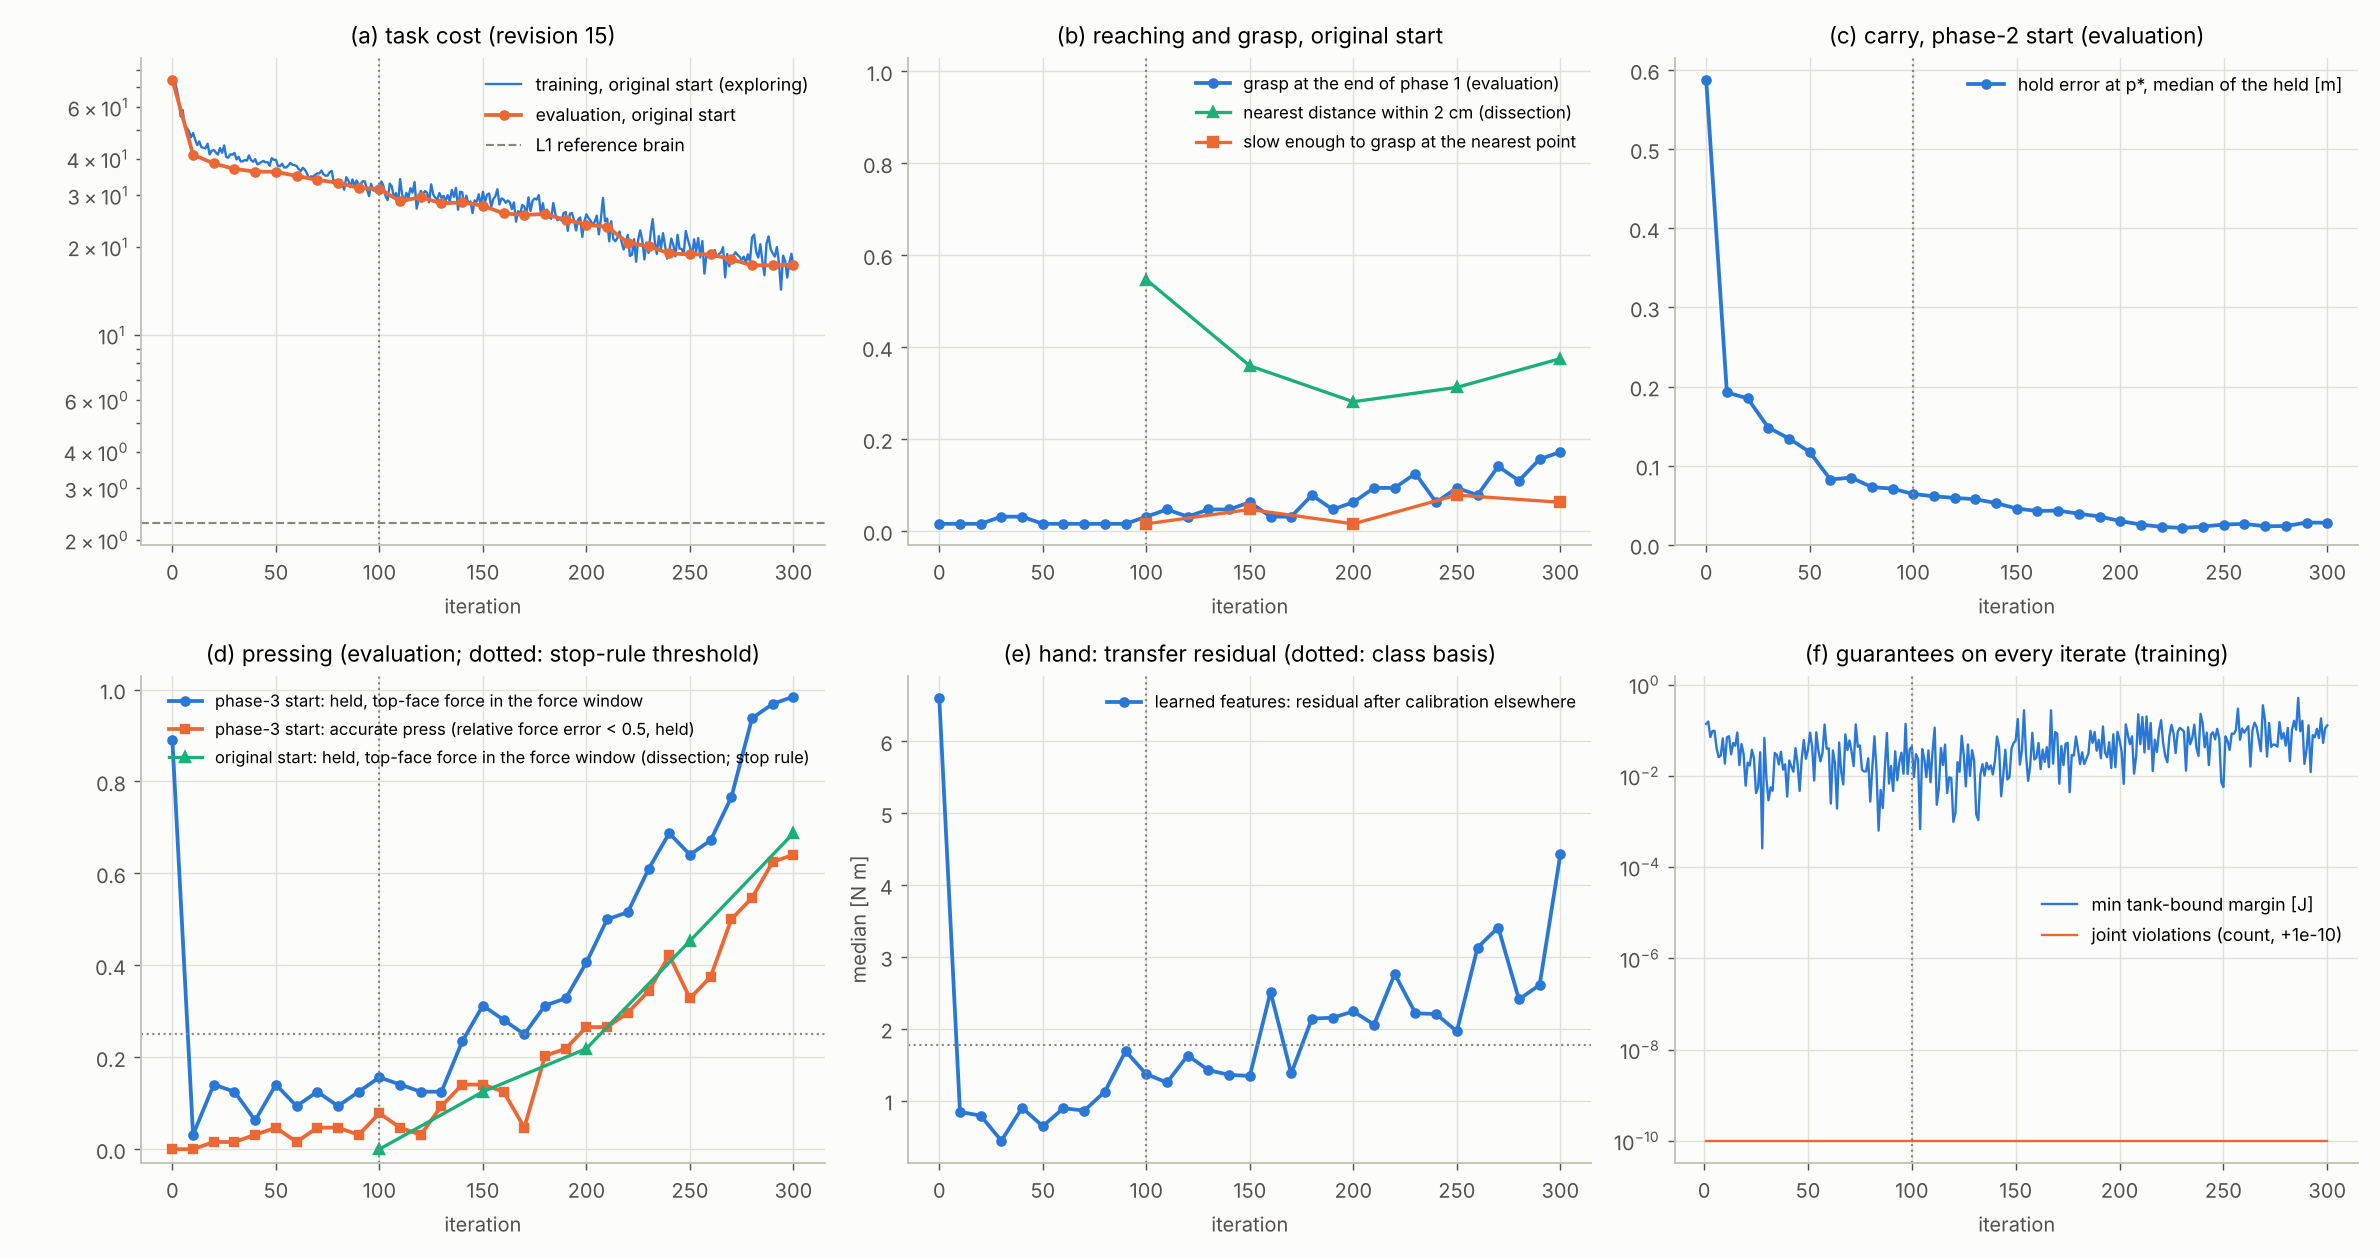
\includegraphics[width=\textwidth]{l2_attempt3.png}
\caption{L2 attempt 3: learning to iteration 300}
\label{fig:l2a3}
\end{figure}

\textbf{결과 (반복 300, \Cref{fig:l2a3}).}
\begin{itemize}
\item \textbf{(G) 충족.} 반복 1--300의 모든 iterate에서 관절 위반 0, 유한하지 않은 상태 0이고, tank 하한 여유의 최솟값은 $2.6\cdot10^{-4}$ J였다. $T_{\min}$ 아래로 포화한 episode는 없었다.
\item \textbf{(H1) 불충족.} 평가 260--300의 다른 자세로 옮긴 오차의 중앙값은 3.130, 3.408, 2.408, 2.609, 4.427 N\,m이고 평균은 3.196 N\,m였다(기준 1.768). 평가 110--150의 평균은 1.400이었다.
\item \textbf{(H2) 불충족.} 기준 뇌를 학습된 손으로 돌린 등급 결정은 0.922(64개 가운데 59개)였다. 반복 100, 150, 200, 250에는 0.969, 0.953, 0.938, 0.922였다.
\item \textbf{중단 규칙은 적용되지 않았다.} $\mu_0$의 평가 episode 가운데 든 채 힘 구간에서 윗면을 누른 것은 64개 가운데 44개(68.8\%)였다. 반복 100, 150, 200, 250에는 0, 12.5, 21.9, 45.3\%였다.
\item \textbf{뇌: 옮기기와 누르기.} $\mu_2$에서 $p^\star$의 유지 오차는 0.0278 m였고(반복 100, 150, 200, 250에 0.0642, 0.0458, 0.0300, 0.0256 m), 64개 모두 단계 3까지 들었다. $\mu_3$에서 정확히 누른 몫은 0.641이었고(0.078, 0.141, 0.266, 0.328), 64개 가운데 63개가 닿았으며 닿은 경우의 힘은 중앙값 $0.74f^\star$(90 백분위 $1.51f^\star$)였다.
\item \textbf{뇌: reaching.} $\mu_0$에서 단계 1 끝의 잡기는 0.172, 최근접 거리의 중앙값은 0.0291 m, 2 cm 안에 든 몫은 0.375, 가장 가까운 순간에 잡을 만큼 느린 몫은 0.062였다. 단계 3에 물체를 든 episode는 45개였다(단계 1 뒤의 잡기 포함).
\item \textbf{학습 신호 (512 episode).} 단계 2의 $p^\star$ 방향은 반복 200에 $0.024$ $[-0.024,\ 0.078]$, 300에 $0.075$ $[-0.006,\ 0.187]$이고, 단계 3의 $p_c$ 방향은 $-0.010$ $[-0.071,\ 0.046]$, $0.022$ $[-0.012,\ 0.057]$이었다. 네 구간 모두 0을 포함한다. 목표 방향 편차의 표준편차는 0.0052--0.0070 m였다.
\end{itemize}

\textbf{분해 1: 등급 결정 (기술, 등록하지 않음).} 반복 300에 닿은 episode의 등급 결정은 $\mu_2$에서 0.452(62개), $\mu_3$에서 0.460(63개), $\mu_0$에서 0.455(11개)로 우연 수준이었다. 장부에는 등급이 있었다. 평가 episode에서 단계 3의 마지막 든 결정의 장부 부하를 L1의 규칙(손끝 부하가 $M_{\mathrm{th}}g$보다 크면 무거움)으로 읽으면 45개 가운데 0.911이 맞았다(반복 100에는 11개 가운데 1.000, \texttt{records/l2\_ledger\_check.json}). 단계 3에서 장부의 질량은 참값보다 중앙값으로 0.13--0.19 kg 작았다. 뇌는 장부를 쓰지 않고 두 등급의 목표 사이의 힘으로 누른다. 이 결정의 값은 작다. L1에서 장부를 쓴 기준 뇌의 평균 비용은 2.290, 장부를 가린 기준 뇌는 2.520이었고(차이 0.230), 반복 300의 학습된 뇌의 평가 비용은 17.370이다.

\textbf{분해 2: 손 (사후 분석, 등록하지 않음).}
\begin{itemize}
\item \textbf{같은 data에서의 role loss.} 반복 200 뇌의 rollout(처음 시작 64개, 단계 3 시작 64개)을 손 100, 140, 200으로 replay하면, 가중 role loss는 처음 시작에서 1.153, 1.146, 1.188이고 단계 3 시작에서 0.747, 0.816, 0.647이었다(\texttt{records/l2\_hand\_replay.json}). 세 손의 다른 자세로 옮긴 오차는 1.366, 1.357, 2.241 N\,m이다. Role loss는 세 손을 거의 구별하지 않고, 옮김은 구별한다. 학습 중의 role loss가 반복 121--140의 평균 0.711에서 201--220의 0.927로 오른 것은 data가 바뀐 결과이다. 같은 구간에 단계 3에 든 episode가 닿은 몫은 0.342에서 0.633이 되었다. 단계 3 시작에서 닿은 step은 전체의 16\%이고, 가중 role loss의 37--40\%를 차지했다.
\item \textbf{오프라인 학습.} 반복 140의 손을 optimizer 상태와 함께 학습과 같은 방식(반복마다 Adam 16 step, 32 episode)으로 30 반복 더 학습했다. 반복마다 고정된 뇌로 새 batch를 만들고, 모든 변형이 같은 batch를 본다(\texttt{records/l2\_hand\_fresh\_b140.json}, \texttt{l2\_hand\_fresh\_b300.json}). 옮긴 오차는 시작에 1.357이었고, 5 반복마다 다음과 같았다.
\begin{itemize}
\item 반복 140 뇌의 data: 1.886, 2.291, 1.257, 2.092, 1.964, 2.111(평균 1.934).
\item 반복 300 뇌의 data: 2.935, 2.280, 2.491, 3.563, 3.103, 4.126(평균 3.083).
\item 반복 300 뇌의 data에서 닿은 step을 role loss에서 뺀 경우: 2.444, 1.839, 2.896, 2.702, 3.121, 5.111(평균 3.019).
\end{itemize}
고정된 6개 batch를 거듭 쓴 60 반복의 실험에서도 결과는 같았다. 옮긴 오차는 모든 step 3.691, 닿은 step을 뺀 경우 2.637, 접촉의 시작과 끝을 짐의 변화로 다룬 경우 3.095였다(\texttt{records/l2\_hand\_contact.json}).
\item \textbf{옮김을 시험하는 data.} 물체를 든 채 기억이 멈춘 상태로 마지막 정지 자세에서 0.2 rad 넘게 움직인 step이 role 가중치에서 차지하는 몫은, 반복 100, 140, 200, 300의 뇌에서 0.018, 0.028, 0.077, 0.025였다(\texttt{records/l2\_transfer\_exposure.json}). 움직이는 step 전체의 몫은 0.698, 0.645, 0.633, 0.506이었다.
\end{itemize}

\textbf{해석.} 채택한 구성에서 뇌는 옮기기와 누르기를 배웠다. 반복 100에 $p_c$ 위에 떠 있던 뇌가 반복 300에는 $\mu_3$의 64개 가운데 63개에서 눌렀다. 학습 신호 진단은 이 개선을 잡지 못했다. 이 진단은 목표 방향의 편차와 advantage의 상관만 보므로, 개선은 다른 경로로 일어났을 수 있다. 뇌는 등급 결정을 아직 배우지 않았다. 장부에 정보는 있지만, 이 결정의 값(L1에서 episode당 0.230)은 학습된 뇌의 평가 비용 17.370에 비해 작다.

손은 역할을 잃었다. Role loss는 rollout 안의 오차를 재고, 그 오차는 정지할 때마다 기억이 다시 맞추면 작아진다. 따라서 한 자세의 보정이 다른 자세로 옮겨 가는지는 role loss에 약하게만 걸린다. 같은 data에서 role loss가 거의 같은 세 손의 옮긴 오차는 1.36에서 2.24까지 달랐다. 반복 140 뇌의 data로 학습을 이어도 옮김은 나빠졌고, 반복 300 뇌의 data에서는 더 나빠졌다. 닿은 step을 빼도 표류는 그대로였으므로 접촉은 원인이 아니다. \Cref{sec:l2a1} 이후의 가중치는 기억이 지울 수 있었던 몫만 손에 묻는다. 그러나 옮김을 손의 몫으로 남긴다는 설계(\Cref{lem:restfloor}의 해석)는 loss에 따로 들어 있지 않고, 뇌의 행동이 만드는 data에 맡겨져 있었다. 각 parameter가 제 역할을 배우게 하는 학습 체계라는 이 연구의 질문에서, 이것이 지금 가장 큰 결함이다.

\textbf{제안 (추가하지 않음, 승인 대기).} 옮김을 손의 role loss에 명시한다. Replay의 한 episode 안에서 같은 짐을 든 두 자세 $q_a$, $q_b$를 뽑아, $q_a$에서 기억이 수렴했을 보정을 $q_b$로 옮긴 오차를 더한다.
\[
\mathcal L_{\mathrm{tr}}=\mathbb E_{a,b}\,\big\|G(q_b)^\top(\bar a+z_a^\star)-u^\star_b\big\|^2,\qquad z_a^\star=G(q_a)\big(G(q_a)^\top G(q_a)+\epsilon I\big)^{-1}\big(u^\star_a-G(q_a)^\top\bar a\big)
\]
$z_a^\star$는 정지한 기억의 고정점(최소 norm)이고, $u^\star$는 지금의 role loss가 이미 쓰는 privileged 신호이다. 새 정보나 instance 모형을 넣지 않고, 이미 선언한 손의 역할을 loss로 옮기는 것이다. 먼저 위의 오프라인 학습(반복 300 뇌의 새 data, 30 반복)으로 시험한다. 평가 쌍과, 학습에 쓰지 않은 자세 쌍에서 옮긴 오차가 1.768 아래에 머물고 role loss가 10\% 넘게 오르지 않으면, 반복 300에서 이어 도는 pilot으로 간다.

\subsection{반복 300의 학습 상태}
\label{sec:l2status}

\Cref{fig:l2status}와 아래 수치는 학습 없이 기록과 결정론적 rollout으로 얻었다(\texttt{records/l2\_traj\_check.json}, \texttt{l2\_never\_rest.json}).

\begin{figure}[H]
\centering
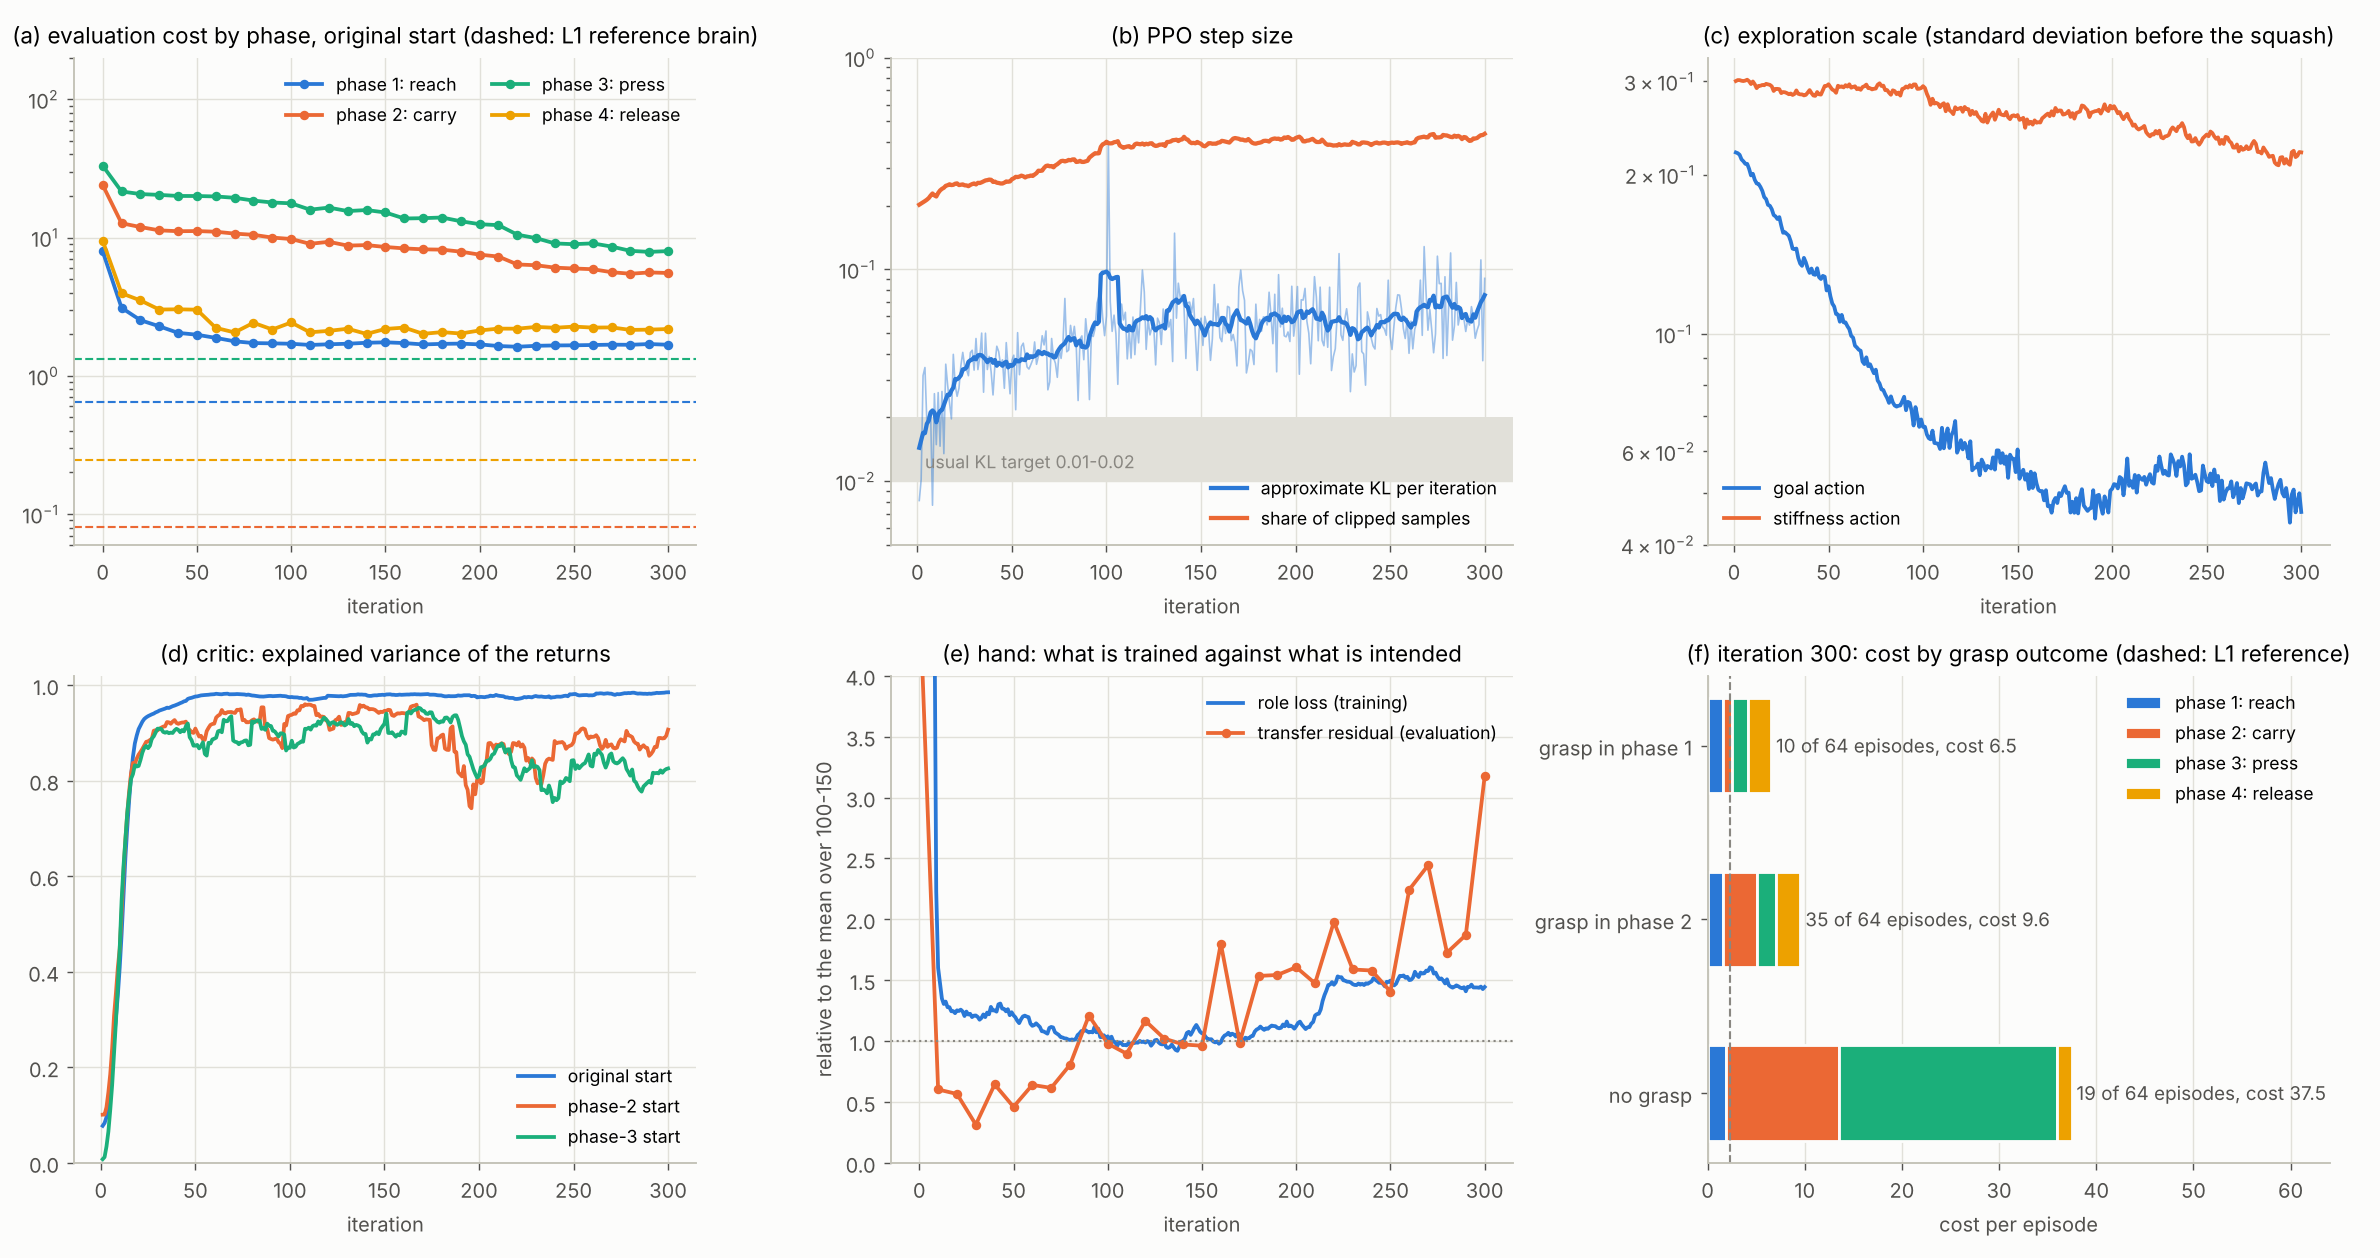
\includegraphics[width=\textwidth]{l2_status.png}
\caption{Learning status at the end of L2 attempt 3}
\label{fig:l2status}
\end{figure}

\textbf{최적화.}
\begin{itemize}
\item 평가 비용은 반복 0, 100, 300에 74.41, 31.55, 17.37이었고, L1의 기준 뇌는 2.290이다. 64개 평가 episode의 평균 비용의 표준오차는 1.69이다.
\item 훈련 비용의 반복당 기울기는 반복 101--200에 $-0.066$, 201--300에 $-0.057$, 251--300에 $-0.024$였다.
\item 반복 101--300의 반복당 approximate KL의 중앙값은 0.0555이고, clip된 표본의 몫은 중앙값 0.40이었다. 반복 1--10의 평균은 0.019와 0.217이었다.
\item 표준편차(squash 전)의 평균은 goal 행동이 반복 1--10의 0.211에서 261--300의 0.0507로, 강성 행동이 0.300에서 0.221로 줄었다.
\item Critic이 설명한 return의 분산은 반복 261--300에 처음 시작 0.983, 단계 2 시작 0.879, 단계 3 시작 0.821이었고, 단계 4의 결정에서는 0.650이었다.
\item L2의 모든 run은 같은 PPO hyperparameter(학습률 $3\cdot10^{-4}$, 5 epoch, minibatch 4096 결정, clip 0.2, entropy 계수 $10^{-3}$)와 반복당 128 episode를 썼다.
\end{itemize}

\textbf{잡기.} 잡은 시점에 따라 나눈 평균 비용은 단계 1에 잡은 10개가 6.539, 단계 2에 잡은 35개가 9.559(단계 2 시작 뒤 지연의 중앙값 0.5 s), 잡지 못한 19개가 37.460이었다.
\begin{itemize}
\item 잡지 못한 episode는 2 cm 안에 한 번이라도 든 몫이 0.158이고 최근접 거리의 중앙값이 0.0288 m였다. 잡는 점은 반경 0.733 m, 높이 0.275 m(중앙값)로, 단계 1에 잡은 episode의 0.482 m, 0.040 m보다 멀고 높았다.
\item 단계 1에서 잡는 점 2 cm 안에 있던 결정의 관절 속도는 중앙값 0.332 rad/s였고, 잡기의 속도 조건(0.1 rad/s)을 만족한 결정의 몫은 0.044였다. 2 cm 안에서 뇌가 명령한 이동 $\|\Delta p\|$의 중앙값은 0.0253 m였다.
\end{itemize}

\textbf{누르기.} 처음 시작에서 윗면에 힘을 낸 44개의 힘 구간 평균 힘 $\bar f$를 두 등급의 목표와 등급 항으로 회귀했다. $h\in\{0,1\}$은 무거운 등급의 표시이다.
\[
\bar f\approx-1.556+0.369\,f_{\mathrm{light}}+0.544\,f_{\mathrm{heavy}}-0.038\,h\,(f_{\mathrm{heavy}}-f_{\mathrm{light}})
\]
상대 오차의 중앙값은 0.370이고, 두 목표의 중간 힘으로 눌렀다면 0.330이다.

\textbf{놓기.} 단계 4에 물체를 든 45개 가운데 결정론적 평가(logit $>0$)에서 놓은 몫은 0.089였다. 같은 정책에서 gripper를 표본으로 뽑으면 1.000이 놓았고, 지연의 중앙값은 0.15 s였다. 단계 4에서 든 동안 여는 확률은 0.252이므로, 표본으로는 놓고 결정론적 평가에서는 놓지 않는다. 단계 4의 비용은 결정론적 평가에서 2.179, 표본에서 1.495였다.

\textbf{해석.} 남은 비용의 대부분은 잡기에서 온다. 잡지 못한 episode는 멀고 높은 물체에 몰려 있고, 잡은 episode도 잡는 점을 지나쳐 정지하지 못해 대부분 단계 2에 들어가서야 잡는다. 단계 1의 비용은 거리만 재고 속도를 재지 않으므로, 정지해야 한다는 신호는 잡은 뒤의 비용 차이로만 들어온다. 누르는 힘은 두 목표의 가중 평균이고 등급 항은 0에 가깝다. 장부를 쓰지 않는 정책이 낼 수 있는 한계에 가깝다. goal 행동의 탐색 표준편차가 약 4분의 1로 줄어든 뒤에도 학습률이 고정이어서 반복당 KL은 흔히 쓰는 목표(0.01--0.02)의 세 배에서 다섯 배가 되었고, 표본의 40\%가 clip되었다. 반복당 진전이 clip에 묶였을 가능성이 있으나 시험하지 않았다. 결정론적 평가는 놓기를 과소평가하므로 이 절 이전의 단계 4 비용은 정책의 수행보다 높게 기록되었다.

\textbf{다음 단계의 제안 (추가하지 않음, 승인 대기).}
\begin{enumerate}[label=(\arabic*)]
\item 계산 환경을 GPU로 옮기고, 반복 300의 평가를 재현한 뒤 batch 크기별 처리량을 잰다(\texttt{script/port\_check.py}).
\item 평가에 gripper를 표본으로 뽑는 평가를 병기하고, 판정용 평가의 episode 수를 늘린다.
\item 최적화를 짧은 pilot으로 시험한다: 반복당 episode 수, KL에 맞춘 학습률, entropy 계수.
\item 손의 role loss에 옮김 항을 넣고 오프라인으로 먼저 시험한다(\Cref{sec:l2a3}의 제안).
\item (3)의 결과를 본 뒤 잡기의 관문(단계 1 비용의 속도 항 또는 물체 근처의 시작 상태)과 장부의 task 공간 표현을 정한다.
\end{enumerate}

\subsection{접촉력 상한의 상수와 수치 확인}
\label{sec:contactnum}

\textbf{직관 (지금 구조로 닫히는가).} \Cref{thm:closure}의 상수를 Stage B의 plant class와 block 윗면($n=(0,1)$, 접촉점은 손끝)에 대해 표본으로 구했다. 상태는 $\overline{\mathcal X}$에서 뽑고, 손끝이 block 윗면이 놓일 수 있는 영역 $[0.20,0.90]\times[-0.30,0.30]$ m에 있는 것만 남겼다. 경우마다 표본은 200{,}000개이다. \Cref{tab:forceconst}의 값은 표본의 최솟값과 최댓값이므로 참값의 추정이며 증명이 아니다.

\begin{table}[H]
\centering\footnotesize
\caption{Sampled constants of the contact force bound for the Stage B structure}
\label{tab:forceconst}
\begin{tabular}{lcccc}
\toprule
 & \multicolumn{2}{c}{in distribution} & \multicolumn{2}{c}{out of distribution} \\
 & no object & object attached & no object & object attached \\
\midrule
states in the region & 87{,}088 & 87{,}074 & 87{,}147 & 86{,}588 \\
$\min n^\top\Upsilon n$ [1/kg] & 0.1541 & 0.1208 & 0.1332 & 0.1061 \\
$\min\theta$, $\bar\nu_e=0.5$ [1/kg] & 0.0587 & 0.0812 & 0.0240 & 0.0824 \\
$\min\theta$, $\bar\nu_e=0.8$ [1/kg] & $-0.0789$ & $-0.0127$ & $-0.1588$ & 0.0379 \\
share with $\theta\le0$, $\bar\nu_e=0.8$ & 0.00914 & 0.00003 & 0.01044 & 0 \\
$\max\|J_c\dot q\|$ [m/s] & 3.749 & 3.548 & 3.803 & 3.728 \\
$\max a_{\mathrm{in}}$ over $\tau\in\U$ [m/s$^2$] & 243.2 & 195.3 & 317.6 & 161.6 \\
$\max a_{\mathrm{in}}$ under relief, $\|J_c\dot q\|\le0.5$ m/s [m/s$^2$] & $-60.5$ & $-22.1$ & $-44.9$ & $-11.1$ \\
\bottomrule
\end{tabular}
\end{table}

``Under relief''는 $J_c^\top n$ 방향으로 입력 상자에 포화된 torque를 줄 때의 $a_{\mathrm{in}}$이다.

\textbf{지금 구조의 상한.} 분포 안의 class에서 두 하중 경우 중 불리한 값을 쓰면 $\bar\nu_e=0.5$에서 $\underline\theta=0.0587$ kg$^{-1}$, $\bar v_c=3.749$ m/s, $\bar a_{\mathrm{in}}=243.2$ m/s$^2$이다. $\bar\delta_e=5$ s/m에서 \Cref{thm:closure}의 상한은 다음과 같다.
\[
\frac{\bar a_{\mathrm{in}}}{\underline\theta}=4144.6\ \mathrm N,\qquad \sqrt{\bar k_e\,\bar v_c^2/\underline\theta}=2188.8\ \mathrm N\ \ (\bar k_e=2\times10^4\ \mathrm{N/m}),
\]
\[
\bar f_n=1.744\times10^5\ \mathrm N\ \ (\bar k_e=2\times10^4\ \mathrm{N/m}),\qquad \bar f_n=2.411\times10^5\ \mathrm N\ \ (\bar k_e=2\times10^5\ \mathrm{N/m}) .
\]
\Cref{thm:r1}의 (B3)를 인증한 힘은 60 N이므로 조건 $\bar f_n<\bar f_B$는 성립하지 않는다. 원인은 둘이다. 지금 구조가 주는 속도의 상한은 제약층의 gauge에서 나오는 값뿐이고, 접촉 중 구동의 상한은 입력 상자뿐이다. 구동의 상한이 입력 상자이면 $2\bar a_{\mathrm{in}}/\underline\theta$가 이미 60 N을 넘으므로 어떤 속도 한도로도 닫히지 않는다.

\textbf{결정 (2026년 11월 17일).} Contact-permitting constraint를 요구 사항에 넣는다 (R17). 표면의 class는 강성 $2\times10^5$ N/m까지 넓히고 $10^6$ N/m까지도 대상으로 본다. 마찰 계수는 0.8까지 class에 둔다. 힘의 한도는 60 N보다 올린다. 아래 세 문단은 이 결정이 구조에 요구하는 것이다.

\textbf{힘의 한도와 (B3).} \Cref{thm:closure}의 $\bar f_B$는 (B3)가 성립하는 힘이어야 한다. \Cref{sec:envcheck}의 표본(경우마다 40{,}000개, $\nu_e\le0.8$)에서 힘의 한도만 바꾸어 (B3)를 다시 계산했다. 60 N에서는 여유 27.46과 7.40 rad/s$^2$가 재현되고, 100 N에서는 $-125.95$와 $-176.49$ rad/s$^2$로 조건이 깨진다. 표본에서 (B3)가 성립하는 가장 큰 법선 힘 $F^\star$는 \Cref{tab:authority}와 같다. 가속도가 접촉력에 대해 affine이므로 $F^\star$는 표본마다의 값의 최솟값으로 정확히 계산된다.

\begin{table}[H]
\centering\footnotesize
\caption{Largest normal force at which the sampled condition (B3) holds}
\label{tab:authority}
\begin{tabular}{lcccc}
\toprule
 & \multicolumn{2}{c}{margin without contact [rad/s$^2$]} & \multicolumn{2}{c}{$F^\star$ [N]} \\
$\bar u$ [N\,m] & in distribution & out of distribution & in distribution & out of distribution \\
\midrule
(120, 60, 25) & 27.86 & 18.03 & 79.20 & 71.79 \\
(150, 75, 40) & 40.53 & 27.57 & 100.59 & 101.04 \\
(180, 90, 50) & 53.20 & 37.11 & 120.07 & 119.81 \\
(240, 120, 60) & 78.53 & 56.19 & 157.89 & 157.37 \\
\bottomrule
\end{tabular}
\end{table}

지금의 입력 상자 $(120,60,25)$ N\,m에서 $F^\star$는 분포 안 79.20 N, 분포 밖 71.79 N이다. 힘을 접촉 영역의 표본에만 주어도 79.20 N과 73.43 N으로 거의 같다. 접촉 자세에서 torque $J_c^\top n\,f$가 입력 상자에 드는 가장 큰 법선 힘은 최소 100.0 N, 중앙값 138.3 N이다. 따라서 힘의 한도는 입력 상자가 정한다. 지금의 actuator로는 약 72 N까지이고, 입력 상자를 $(240,120,60)$ N\,m로 키워도 157 N이다.

\textbf{필요한 속도 한도.} \Cref{tab:forcespeed}는 \Cref{cor:reaction}의 상한이 힘의 한도와 같아지는 접촉점의 속도 한도이다. 상수는 분포 안 class의 가장 불리한 자세의 값($\underline\theta=0.0587$, $a_r=22.14$ m/s$^2$, $\bar\delta_e=5$ s/m)이고, $t_d$는 제어 주기 둘(4 ms)과 하나(2 ms)이다. \Cref{fig:forcespeed}는 $t_d=4$ ms에서 상한을 속도 한도에 대해 그린 것이다.

\begin{table}[H]
\centering\footnotesize
\caption{Speed limit of the contact point [m/s] that keeps the force bound at a force limit}
\label{tab:forcespeed}
\begin{tabular}{lcccccc}
\toprule
 & \multicolumn{2}{c}{force limit 60 N} & \multicolumn{2}{c}{100 N} & \multicolumn{2}{c}{200 N} \\
$\bar k_e$ [N/m] & $t_d=4$ ms & 2 ms & 4 ms & 2 ms & 4 ms & 2 ms \\
\midrule
$2\times10^4$ & 0.191 & 0.216 & 0.246 & 0.273 & 0.342 & 0.370 \\
$2\times10^5$ & 0.048 & 0.067 & 0.069 & 0.091 & 0.109 & 0.134 \\
$10^6$ & 0.013 & 0.022 & 0.021 & 0.033 & 0.037 & 0.054 \\
\bottomrule
\end{tabular}
\end{table}

\begin{figure}[H]
\centering
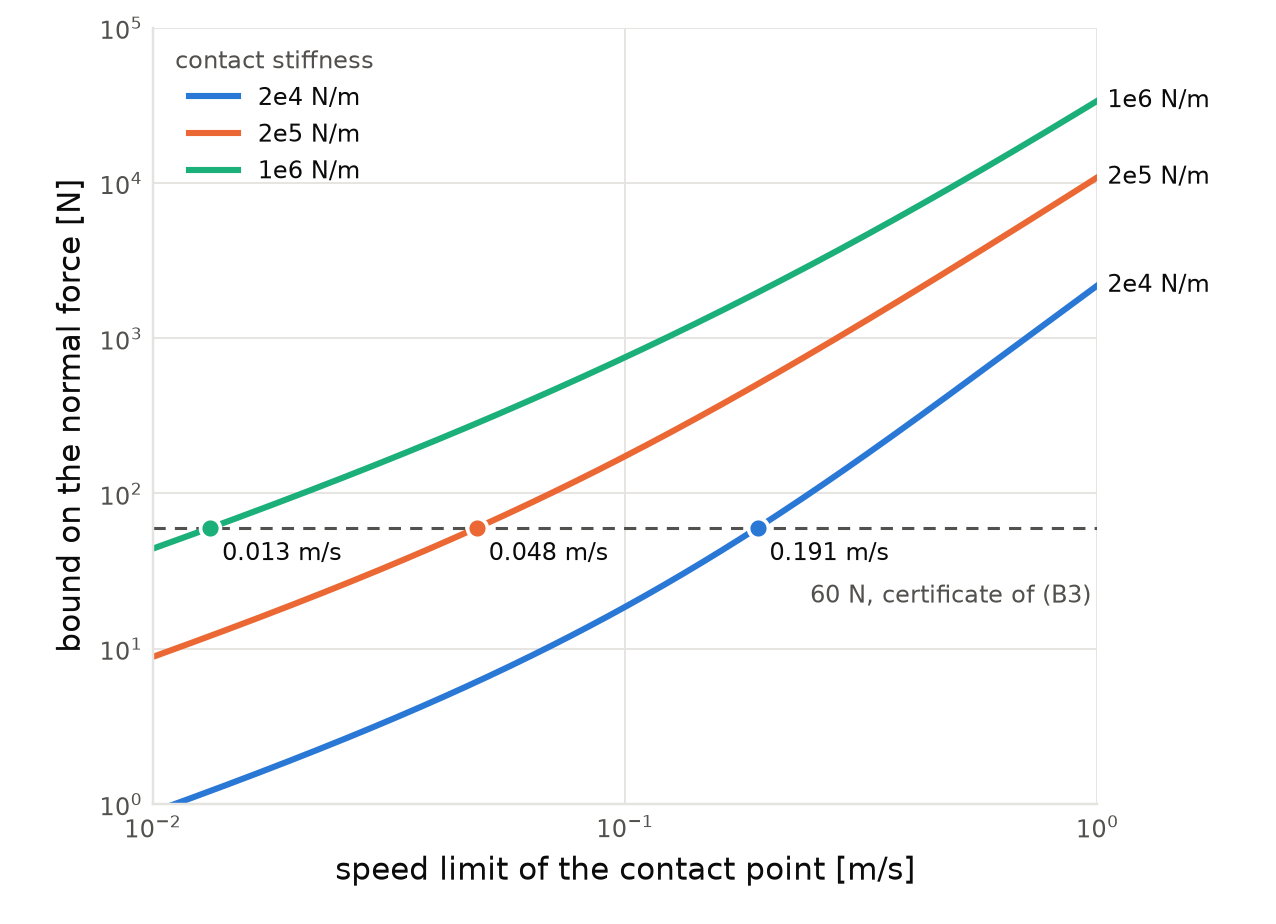
\includegraphics[width=0.72\textwidth]{force_speed_design.png}
\caption{Force bound against the speed limit of the contact point}
\label{fig:forcespeed}
\end{figure}

강성 $2\times10^5$ N/m를 60 N으로 지키는 속도 한도는 0.048 m/s이고 $10^6$ N/m에서는 0.013 m/s로, 과제를 하기 어려운 값이다. 이때 한도를 정하는 것은 감지 지연 동안의 침투 $\bar k_e\,\bar v\,t_d$이다. 힘의 한도를 200 N으로 올려도 0.109 m/s와 0.037 m/s이며, 그 힘은 지금의 입력 상자에서 (B3)를 깨뜨린다. 속도 한도를 과제에 쓸 수 있는 크기로 두는 수단은 접촉점의 강성을 구조가 제한하는 것이다. 접촉점에 강성 $k_p$의 탄성 요소가 직렬로 있으면 탄성 표면과의 합성 강성은 $k_pk_e/(k_p+k_e)\le k_p$이므로, 표면의 강성이 얼마이든 $\bar k_e$의 자리에 $k_p$가 들어간다. $k_p=2\times10^4$ N/m이면 60 N에서 0.191 m/s이다. 이 요소는 torque sensing과 같이 plant class에 넣는 구조이며, 표면의 소산 $\delta_e$가 직렬로 놓일 때의 힘 법칙은 \Cref{def:surface}의 형태가 아니어서 그 경우의 증명은 없다.

\textbf{마찰 계수 0.8.} $\bar\nu_e=0.8$에서 $\theta(q)$는 분포 안에서 물체를 들지 않은 자세의 0.914\%, 든 자세의 0.003\%에서 0 이하여서 (F1)이 class 전체에서는 성립하지 않는다. $\theta$의 1\%, 5\%, 50\% 분위는 들지 않은 자세에서 0.0035, 0.1004, 0.3937 kg$^{-1}$이고 든 자세에서 0.0908, 0.1480, 0.2993 kg$^{-1}$이다. 5\% 분위의 값으로 계산한 속도 한도는 60 N, $t_d=4$ ms에서 0.193, 0.049, 0.013 m/s로 \Cref{tab:forcespeed}와 거의 같다. 곧 $\theta$가 그 값 이상인 자세에서는 마찰 계수 0.8이 속도 한도를 바꾸지 않는다. $\theta\le0$인 자세에는 \Cref{prop:energyforce}만 적용된다. 힘의 한도 $\bar f_c=60$ N에 해당하는 표면의 에너지 $\bar f_c^2/(2\bar k_e)$는 강성 $2\times10^4$, $2\times10^5$, $10^6$ N/m에서 0.09, 0.009, 0.0018 J이다. Gauge 집합에서 팔의 운동 에너지는 최대 9.361 J(물체를 들면 16.852 J)이고, 손끝 속도가 0.5 m/s 이하인 상태로 한정해도 2.576 J과 2.454 J이다. 손끝의 속도 한도만으로는 팔 전체의 운동 에너지가 제한되지 않는다.

\textbf{해석 (세 결정이 요구하는 것).} 힘의 한도는 입력 상자에 묶여 있어 지금의 actuator로는 약 72 N이 끝이다. 단단한 표면을 class에 넣는 것은 접촉점의 탄성 요소 없이는 속도 한도를 수 cm/s로 떨어뜨린다. 마찰 계수 0.8은 $\theta$가 5\% 분위 이상인 자세에서 속도 한도를 바꾸지 않지만, $\theta\le0$인 자세에서는 법선 방향의 논증이 서지 않고 에너지 형태의 상한이 팔 전체의 운동 에너지와 접촉 중 tank의 지불을 제한할 것을 요구한다. 그래서 정할 것은 셋이다. (i) 힘의 한도를 약 70 N에 두고 입력 상자를 유지할지, 입력 상자를 키워 한도를 올릴지. (ii) 접촉점의 탄성 요소를 plant class에 넣을지와 그 강성 $k_p$. (iii) $\theta\le0$인 자세를 관절 속도의 한도와 접촉 중 tank 지불의 한도로 다룰지, 그 자세를 제외하는 regional 결과로 둘지.

\textbf{결정 (2026년 11월 17일, 위 계산을 본 뒤).} (i) 입력 상자 $(120,60,25)$ N\,m를 유지하고 힘의 한도를 $\bar f_c=70$ N으로 둔다. 이 값은 표본의 $F^\star$보다 작다. (ii) 접촉점에 강성 $k_p=2\times10^4$ N/m의 탄성 요소를 두고 plant class에 넣는다. (iii) $\theta\le0$인 자세는 우선 제외한 regional 결과로 두고, 관절 속도의 한도와 접촉 중 tank 지불의 한도로 닫는 것은 다음 단계로 둔다. 세 결정은 아직 구현과 인증에 반영되지 않았다. Stage B의 plant와 학습은 바뀌지 않았고, 속도 한도와 밀어내는 요소, 탄성 요소가 있는 접촉 법칙은 Stage B3에서 넣는다.

\textbf{수치 확인 (부등식).} \Cref{lem:scalar}와 \Cref{thm:force}의 부등식을 임의의 구동에서 확인했다. 합격 기준은 실행 전에 파일로 고정했다(\texttt{records/contact\_bound\_check\_plan.md}, hash 72d4e1cd; 위의 상수는 \texttt{records/contact\_class\_plan.md}, hash a7186461). 비는 관측한 최댓값을 상한으로 나눈 값이며, 1 이하이면 부등식이 성립한다.
\begin{itemize}
\item \textbf{한 자유도.} 질량 0.5--10 kg, 강성 $2\times10^3$--$2\times10^5$ N/m, 구동의 한도 0--100 N, 접촉 시작 속도 0.01--1 m/s에서 구동의 종류마다 2{,}000개를 적분했다. 일정한 구동에 $\delta_e=0$이면 깊이의 비는 중앙값과 최댓값이 소수 여섯 자리까지 1.000000으로, 깊이가 \Cref{thm:force}(a)의 상한에 도달한다. $\delta_e>0$인 일정한 구동과 $\dot d_c$의 부호를 따라 바뀌는 구동에서는 깊이의 비가 최대 0.999634, 힘의 비가 최대 0.998700이었고, 2 ms마다 무작위로 바뀌는 구동에서는 0.967673과 0.943886이었다.
\item \textbf{Stage B plant.} \Cref{sec:envcheck}에서 검증된 plant 모형에 임의의 torque를 넣고 평평한 표면과 부딪히게 했다. 궤적은 3{,}000개이고(분포 안의 몸 2{,}000개, 분포 밖 1{,}000개, 절반은 물체를 든 상태), 표면의 강성은 $2\times10^3$--$2\times10^5$ N/m, torque는 표면 아래의 점을 향한 feedback과 무작위 torque의 두 종류이다. Contact interval마다 그 구간에서 실현된 $\underline\theta$, $\bar a_{\mathrm{in}}$, $V_0$로 상한을 계산했다. Contact interval 13{,}181개 모두에서 $\underline\theta>0$이었고, 깊이의 비는 최대 0.962396, 힘의 비는 최대 0.936738이었다(\Cref{fig:forcecheck}). 관측된 법선 힘은 최대 3822.2 N이다. $\theta\le0$인 구간은 표본에 없었으므로, (F1) 밖의 거동은 이 확인이 다루지 않는다.
\end{itemize}

\begin{figure}[H]
\centering
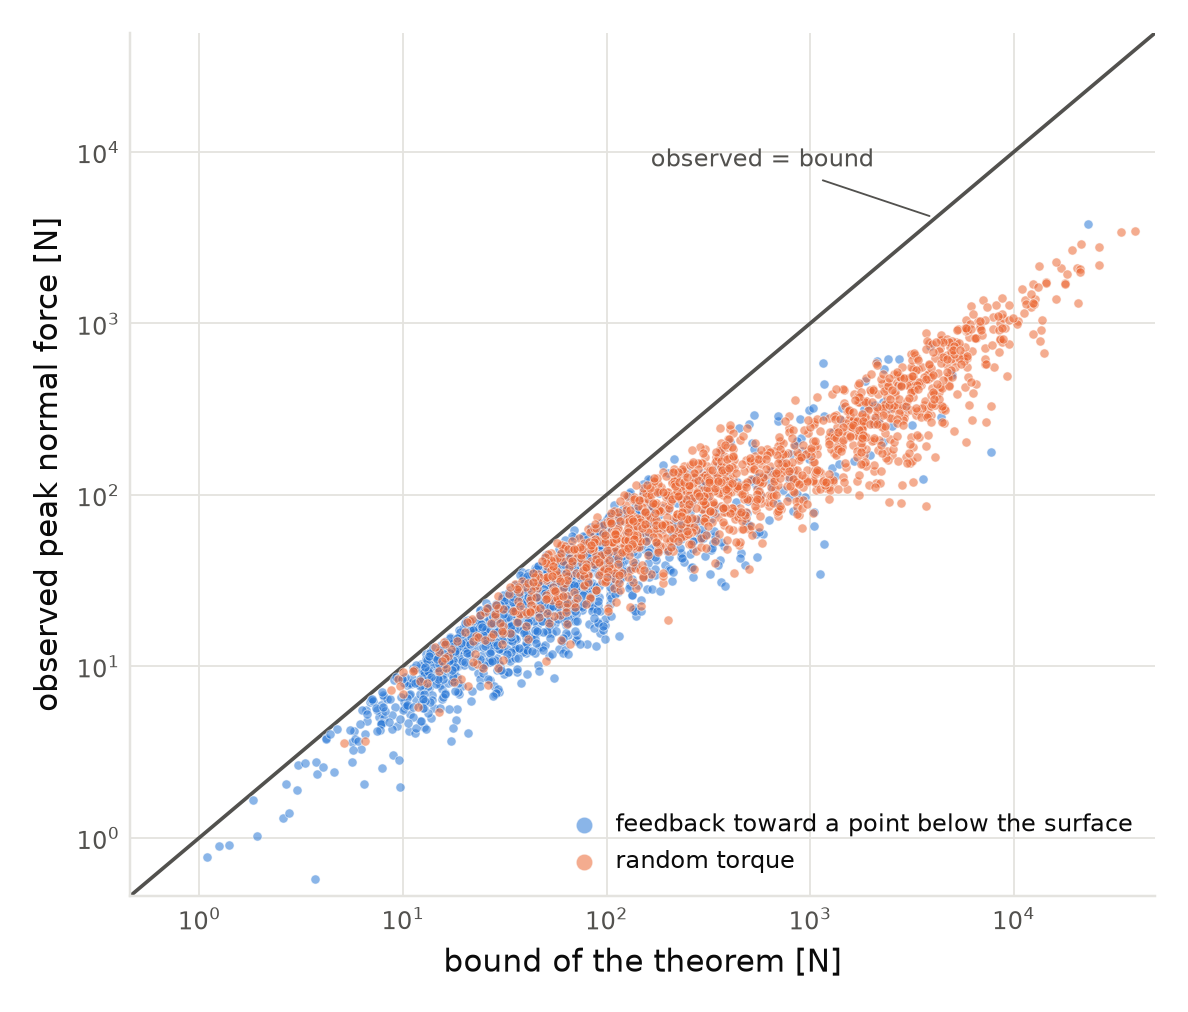
\includegraphics[width=0.62\textwidth]{contact_bound_check.png}
\caption{Observed peak normal force against the bound}
\label{fig:forcecheck}
\end{figure}

\textbf{학습된 정책의 첫 접촉.} 세 번째 시도의 반복 300 checkpoint를 평가 episode 64개에서 결정론적으로 돌려, 첫 접촉 뒤 0.3 s 안의 최대 법선 힘을 쟀다(\Cref{tab:forcepeak}). 단계 3 시작에서 접촉한 63개 가운데 5개가 60 N을 넘었고 최댓값은 106.92 N으로, $F^\star$도 넘는다. 같은 평가에서 관절 위반은 0이었다. (B2)는 충분조건이므로 두 사실은 모순이 아니지만, 그 episode들에서 관절 제약은 \Cref{thm:r1}의 조건 밖에서 지켜진 것이다.

\begin{table}[H]
\centering\footnotesize
\caption{First-contact peak normal force of the learned policy [N]}
\label{tab:forcepeak}
\begin{tabular}{lccccc}
\toprule
start & episodes with contact & median & 90\% & max & share above 60 N \\
\midrule
original & 43 & 14.66 & 32.11 & 57.07 & 0 \\
phase 2 & 60 & 14.24 & 30.35 & 39.88 & 0 \\
phase 3 & 63 & 16.19 & 54.95 & 106.92 & 0.079 \\
\bottomrule
\end{tabular}
\end{table}

\textbf{상태와 남은 것.} \Cref{lem:scalar}, \Cref{thm:force}, \Cref{cor:reaction}, \Cref{prop:energyforce}는 증명되었고, \Cref{thm:closure}는 조건부로 증명되었으나 지금 구조는 그 조건 $\bar f_n<\bar f_B$를 만족하지 않는다. 구조에 없는 것은 둘이다. 접촉점의 속도 한도 (F0)과, 감지된 접촉 뒤에 밀어내는 torque (F2$'$)이다. 두 요소의 형태와, 입력 saturation, 감지 문턱, 잡음, 지연 아래에서 (F0)과 (F2$'$)가 성립한다는 증명이 남아 있다. 속도 한도의 후보는 속도가 한도에 가까워질수록 커지는 감쇠 torque $\tau_v$이며, $\dot q^\top\tau_v\le0$이면 \Cref{def:fulltank}의 수지에서 tank 수준을 줄이지 않는다. 그 밖에 block의 모서리와 옆면, 여러 점의 동시 접촉, sampled-data 구현이 남아 있다. 물체가 표면과 닿는 과제에서는 접촉점이 물체 위의 점으로 바뀐다. \Cref{thm:force}는 접촉점의 $J_c$만 쓰므로 그대로 적용되고 \Cref{tab:forceconst}의 상수만 다시 구하면 된다.

\section{요구 사항}
\label{sec:requirements3}

\textbf{Tier 1: 구성에 의해 성립해야 하는 것.}
\begin{itemize}
\item[\textbf{(R1)}] (\Cref{thm:r1}, under (B1)--(B3)) (Joint constraint) $q(t)\in\mathcal C_q$ $\forall t$.
\item[\textbf{(R2)}] (Input constraint) $\tau(t)\in\U$ $\forall t$.
\item[\textbf{(R3)}] (Gate) $\alpha=0$ whenever $T\le T_{\min}$; hence the hand exchanges no power, $\alpha\,\dot q^\top\tau_h=0$.
\item[\textbf{(R4)}] (Contact passivity) \Cref{thm:fulltank}: the energy identity for every hand, and $T\ge T_{\min}-\bar U_b$ when the saturation is inactive below $T_{\min}$.
\item[\textbf{(R5)}] (Bounded fast weights) $z(t)\in\mathcal Z_0$ $\forall t$.
\item[\textbf{(R6)}] (Learning invariance) (R1)--(R5) for every weight and every iterate of \Cref{def:coupled}; (C1) of \Cref{sec:novelty3} rests on (R1)--(R6).
\end{itemize}

\textbf{Tier 2: 증명할 것.}
\begin{itemize}
\item[\textbf{(R7)}] The tank bound of (R4) with saturation active below $T_{\min}$; the active constraint layer alone is covered by \Cref{lem:barrier}.
\item[\textbf{(R8)}] (Steady-state accuracy) Convergence of the rest calibration of \Cref{def:hand} in closed loop, with the hybrid rest indicator.
\item[\textbf{(R9)}] (Liveness) $T(0)-T_{\min}$ exceeds the task energy, estimated before deployment.
\item[\textbf{(R10)}] (Sampled data) Discrete-time tank, gate and memory that keep (R3)--(R5).
\item[\textbf{(R11)}] (Inexact representation) A bound of the residual supply $\dot q^\top\delta$ by the tank.
\item[\textbf{(R15)}] (Contact force bound) An upper bound of the contact force that does not rely on the energy budget; the static part is \Cref{prop:static}.
\item[\textbf{(R17)}] (Contact-permitting constraint) $\|f_e(t)\|\le\bar f_c$ $\forall t$ for every surface of the class of \Cref{def:surface}, impact included. Proven in terms of the onset speed and the inward drive under (F1) and (F2) (\Cref{thm:force}), with a speed limit and a delayed relief (\Cref{cor:reaction}), and jointly with (R1) when the bound is below the force of (B3) (\Cref{thm:closure}). Open: the elements that give (F0) and (F2$'$), and the configurations with $\theta(q)\le0$.
\end{itemize}

\textbf{Tier 3: 사전 등록해 실험으로 시험할 것.}
\begin{itemize}
\item[\textbf{(R12)}] (Coupling) The coupled framework learns faster and reaches higher success than its ablations.
\item[\textbf{(R13)}] (Contact stability) Stable contact on test stiffness outside the training range.
\item[\textbf{(R14)}] (Performance) Return not below the baselines of \Cref{sec:eval} at zero violations.
\item[\textbf{(R16)}] (Role fidelity) The thresholds of \Cref{def:rvp} are met.
\end{itemize}

\section{평가 사양}
\label{sec:eval}

\textbf{비교 대상 (Stage B).}
\begin{enumerate}[label=(\arabic*)]
\item v3 전체 (\Cref{def:coupled});
\item 뇌가 장부를 보지 못하는 v3;
\item 모든 weight를 하나의 return으로 학습한 v3;
\item 분리 학습: 손을 일반 reference로 먼저 학습해 고정한 뒤 뇌를 학습;
\item 기억이 없는 v3 (impedance, tank, 제약층);
\item 뇌와 같은 결정 주기의 torque 정책 (tank, gate, 제약층을 거침);
\item 제어 주기의 torque 정책 (참고);
\item 내부 기억을 가진 torque 정책 (parameter를 무작위화해 학습);
\item 정해진 뇌 (L1의 상한).
\end{enumerate}

\textbf{예측 후보 (L2의 사전 등록에서 확정).}
\begin{itemize}
\item[\textbf{(P1)}] 분포 밖의 무게와 몸에서 (1)의 과제 오차는 분포 안의 값의 정해진 배수 안에 머물고, (5), (6), (8)은 그 배수를 넘는다. 몸은 \Cref{tab:stageB}대로 질량과 링크 길이를 함께 바꾸고, 원인은 분석에서 나눈다: 질량만 또는 길이만 바뀐 하위 조건, 손의 몫(torque 불일치, 등급 결정)과 뇌의 기구학 몫(손끝 오차). 뇌는 기구학 오차를 비례 보정으로만 줄이므로(\Cref{fact:noint}) 길이가 바뀐 몸에서는 (8)이 (1)보다 작은 위치 오차를 낼 수 있고, 그 결과도 그대로 보고한다.
\item[\textbf{(P2)}] 잡기와 놓기 직후 (1)의 PRI는 문턱 이하이고 (3)의 PRI는 그보다 크다.
\item[\textbf{(P3)}] 누르기 단계에서 (1)은 질량 등급에 맞는 목표 힘을 고르고, 그 힘 오차와 비용은 (2)보다 작다. 예산 episode에서는 장부의 가치를 주장하지 않고 gate의 작동만 확인한다(\Cref{sec:l1pilot}).
\item[\textbf{(P4)}] 학습 범위보다 단단한 block에서 (1)의 접촉 직후 최대 힘과 진동 에너지는 기준 이하이고, (7)은 그렇지 않다.
\item[\textbf{(P5)}] (1)은 (4)보다 적은 학습량으로 (9)의 성능의 정해진 비율에 도달한다.
\end{itemize}
판정 규칙: 관문 L0과 L1을 통과한 뒤에만 L2를 실행한다. 기각된 예측에 딸린 주장은 버리고, 지지된 주장만으로 계속한다. 수치 범위, seed 수, 학습 예산, 문턱은 L2의 사전 등록 파일에서 정한다. Stage A에서의 결과(M1, M2)는 \Cref{sec:m1,sec:m2,sec:m2audit}에 있다.

\section{현재 상태}
\label{sec:status3}

{\footnotesize
\begin{longtable}{p{4.3cm}p{2.6cm}p{7.6cm}}
\caption{Status of the v3 components}\label{tab:status3}\\
\toprule
항목 & 상태 & 비고 \\
\midrule
\endfirsthead
\toprule
항목 & 상태 & 비고 \\
\midrule
\endhead
Passivity, port-Hamiltonian, energy tank의 기본 lemma & 증명 (표준) & \Cref{sec:prelim} \\
손의 에너지 균형 & 증명, 부록으로 이동 & 개정 7의 속도 구동 기억에 대한 결과 (\Cref{app:oldmem}) \\
접촉 port의 passivity & 증명 (범위 제한) & 에너지 항등식은 모든 손에 대해; tank 하한은 $T<T_{\min}$에서 saturation이 없을 때 (\Cref{thm:fulltank,lem:barrier}) \\
작동 중인 제약층과 saturation 아래의 passivity (R7) & 부분 & 제약층은 저장 함수로 포함 (\Cref{lem:barrier}); $T<T_{\min}$에서의 saturation은 미해결 \\
제약층 (R1) & 증명 & gauge 형태, 방향 authority 조건 아래, 잡기 사건 포함 (\Cref{thm:r1}) \\
정상 상태 정확도와 passivity의 양립 (R8) & 부분 & 측정된 mismatch에 의한 calibration; M1에서 정상 상태 mismatch 0.0090 Nm 이하; 수렴 증명은 미해결 \\
접촉 힘 상한 (R15) & 부분 & 정적 상한 (\Cref{prop:static}) 증명, 감지된 접촉에서 $\tau_{\max}$와 mismatch로 제한; 동적 부분은 (R17) \\
Contact-permitting constraint (R17) & 조건부 증명, 조건 미성립 & 접촉력의 상한 (\Cref{thm:force,cor:reaction}), 마찰과 무관한 에너지 형태 (\Cref{prop:energyforce}), 관절 상자와의 결합 (\Cref{thm:closure}). 지금 구조의 상한은 $1.744\times10^5$ N으로 (B3)를 인증한 60 N을 넘음. 속도 한도와 밀어내는 요소가 구조에 없음. (B3)가 성립하는 힘은 71.79 N까지 (\Cref{sec:contactnum}) \\
역할 학습과 검증 (R16) & 정의됨 & \Cref{def:rvp} \\
Torque sensing과 접촉 guard & 정의됨 & 잘못된 calibration의 정상 상태 접촉 torque 12.314--12.449 Nm가 0.605--4.150 Nm로 (수치) \\
구현, 학습, 검증 계획 & 정의됨 & \Cref{sec:plan} \\
M1 기구 검증 & 수정된 구성으로 통과, 반영됨 & 적대적 뇌의 접촉 torque 5.971--6.002 Nm, 최소 tank 1.0467 J (\Cref{sec:m1}) \\
M2 Stage A 결합 학습 & 과제와 보장 성립, 역할 학습 일부 실패 & spring 한도와 치우친 기억을 쓰는 해법; 과제와 검증이 아이디어를 시험하지 못함 (\Cref{sec:m2,sec:m2audit}) \\
과제와 검증의 재설계 & 승인; 접점과 Stage B 반영 & 과제 A$'$, 분포 밖 시험 (\Cref{sec:m2audit}) \\
Stage B 과제 & 정의됨 & 평면 3관절 팔, 잡기 명령, 네 단계, 다시 잡기 허용 (\Cref{sec:stageB}) \\
장부 & 정의됨 & $(T,\bar\lambda,\hat u_{\mathrm{load}})$, 뇌가 계산할 수 있는 항목 제외 (\Cref{def:ledger}) \\
L0 부품 시험 & 고친 구성으로 통과, 반영됨 & 정규화된 기억 갱신, tank 수준 gate, 상수 (\Cref{sec:l0}) \\
L1 pilot & 완료, 제안 승인, 반영됨 & 뇌의 관측에서 $q_d$, $K$ 제외, 예산 $\Delta T+\rho E_{\mathrm{task}}$, 질량 등급의 목표 힘 (\Cref{sec:l1pilot}) \\
L1 과제 타당성 & 사전 등록(hash 5abe91f5), 13개 기준 모두 통과 & 상한, 기억과 장부의 필요성, 보장 장치의 작동; 분포 밖의 몸은 길이에서 실패 (\Cref{sec:l1}) \\
Stage B 환경 & 구현, 검증 통과 & 독립 기준 둘과 대조, 18개 항목 통과; (B3) 표본 여유 27.46(분포 안), 7.40(분포 밖) rad/s$^2$ (\Cref{sec:envcheck}) \\
진행 보장 (R9) & 재정식화 & task energy로 표현, 예산에 중력에 대한 일 포함 \\
결합 학습 framework & 개정 14, 두 번째 시도 완료 & role loss에 정지 시간 가중치 $w$ (\Cref{def:coupled,lem:restfloor}) \\
L2 첫 시도 & 반복 100에서 중단, 진단 완료 & 손의 역할 학습과 장부 경로 작동, 보장은 190 반복 모두 성립; 비용의 결함(놓기 유인, 옆면의 평평한 영역)과 role loss의 귀속 결함 (\Cref{sec:l2a1}) \\
L2 두 번째 시도 & 반복 300에서 중단 규칙 적용, 분해 완료 & (G)와 (H2) 충족, (H1) 미충족(2.947 N\,m); 누르기 0\%; 놓기 유인 없어짐; 두 구성요소의 data 범위가 뇌의 실력에 묶임; 시작 상태 분포의 pilot 제안 (\Cref{sec:l2a2}) \\
과제 비용 (개정 15) & 승인, 반영됨 & 물체의 진척 구조와 누르기 항의 상한 (\Cref{prop:costprog}), V17과 V18로 확인, L1 판정 불변 \\
L2 세 번째 시도 & 완료, (G) 충족, (H1)과 (H2) 불충족 & 옮기기와 누르기를 배움, 손의 옮김이 무너지고 뇌는 장부를 쓰지 않음 (\Cref{sec:l2a3}) \\
L2 pilot T & 완료, task 공간의 행동 채택(개정 16) & 옮기기 오차 T 0.064 m 대 J 0.141 m, 2 cm 안 35개 대 4개(64개 가운데); 느린 도착과 누르기는 미해결; T를 300까지 잇는 세 번째 시도 제안 (\Cref{sec:l2pt}) \\
L2 pilot R & 완료, 채택하지 않음 & 시작 상태 분포 대 그대로; (P) 실패, 뒤 단계의 학습 신호 없음(목표 방향 탐색 1.2--1.6 cm), 손의 오차는 B가 낮음; task 공간 행동의 결정 실험 제안 (\Cref{sec:l2pr}) \\
과제와 평가 & 정의됨 & 수치는 사전 등록에서 \\
Universal approximation (v3) & 미해결 & 뇌의 행동이 impedance setpoint로 제한; 후보는 tank 안의 학습된 반사 torque \\
7-DOF 검증 & 계획됨 & Stage C, (M4) \\
문헌 대조 & 일부 & Zhang 등 전문, Zanella 등 전문 앞부분 확인; Michel 등과 Zhang, Li, Figueroa는 미확인 \\
v2 설계 & 중단 & v2 사양, 제약 노트, 학습 비교 노트 \\
\bottomrule
\end{longtable}
}

\section{기존 연구와 새로움}
\label{sec:novelty3}

\textbf{가장 가까운 연구 (전문).} Zhang, Solak, Hjorth, Ajoudani(2025)는 Cartesian 가변 impedance 제어에 RL을 결합했다. 정책은 end-effector 변위와 강성을 출력하고, passivity는 budget과 flow 제한을 가진 energy tank로 다룬다. 학습 중에는 tank의 budget과 flow 조건을 constrained MDP의 제약으로 넣어 safety critic이 passivity 위험을 배우게 하고, 배치 때는 정책 출력에 passivity layer를 둔다. 정책과 safety critic의 상태는 F/T sensor의 wrench와 end-effector 위치로 정의되어 있고, 하위 impedance controller는 고정이며 온라인 적응은 없다. 저자들은 filter가 정책에게 환경의 일부로 보여 같은 action의 결과가 filter 변수에 따라 달라지는 투명성 문제를 지적한다.

\textbf{그 밖의 관련 연구.} Zanella, Palli, Stramigioli, Califano(2024)는 학습과 추론 모두에서 RL 정책을 energy tank로 passivize한다(초록). Sacerdoti, Benzi, Secchi(2024)는 RL로 tank의 크기를 조절한다(제목). Michel, Saveriano, Lee(2024)는 control barrier function에 기반한 safety-aware tank를 제시한다(제목). Zhang, Li, Figueroa(2024)는 관절 제약을 만족시키며 실행 가능할 때 passive한 상호작용 제어를 증명한다(초록). Shahriari 등(2019)은 tank의 budget만으로는 passivity에 부족하고 flow 제한이 필요함을 보인다(제목과 Zhang 등의 서술).

\textbf{추가 확인 (전문).} Zanella 등(2024)은 임의의 제어 입력을 energy tank로 passivize하고, 과제를 passive하게 끝내는 데 필요한 최소 tank 에너지인 task energy를 정책을 돌려 추정하며, 일정한 torque 아래에서 tank의 에너지 감소를 정확히 계산하는 이산 시간 방법을 쓴다. 또 tank가 정책의 환경을 비Markov로 만든다는 점을 지적하고, tank 상태를 agent의 상태에 넣거나 고갈 시 episode를 끝내는 두 해법을 든다. 따라서 tank 상태를 정책에 관측으로 주는 것은 새롭지 않다. 접촉 제어 문헌에는 tank 에너지를 사람의 의도를 나타내는 지표로 쓰는 예(초록)와, 상호작용 parameter의 적응을 tank로 허용하는 예(초록), task energy 추정으로 tank parameter를 적응시키는 예(Benzi 등 2022, 초록)도 있다. 반면 미지 동역학(부하)을 온라인으로 배우는 적응 기억을 passivity 장부 안에 둔 학습 구조는 찾지 못했다.

\textbf{판정.} 에너지를 인식하고 passivity를 보장하는 RL은 새롭지 않다. 제약과 passivity의 결합도 부분적으로 있다. 우리 구조의 부품도 대부분 기존에 있으므로, 현재 구조를 부품의 조합으로 내세우면 새로움이 약하다.

\textbf{확인된 범위 안에서 남는 차이.}
\begin{enumerate}[label=(\alph*)]
\item 하위 controller 자체가 학습되고 온라인으로 적응하며, 그 적응이 passivity 장부 안에 있다. 위 연구들의 하위 controller는 고정된 impedance이다.
\item 투명성: 위 연구들은 tank를 제약이나 filter로 쓰고, Zhang 등의 상태 정의에는 tank 상태가 없다. 우리는 장부를 정책의 관측으로 주고, 하위층에도 역할 신호를 준다.
\item 양방향성: 뇌의 의도(목표와 강성)가 손의 응답과 calibration의 속도를 정하고, 손의 장부가 뇌의 관측에 들어간다.
\end{enumerate}

\textbf{손의 calibration 법칙과 고전 결과.} 자유 공간에서 gate가 열려 있고 제약층과 saturation이 작동하지 않으면 $\hat m=Ke_q+D_W\dot q-n$이므로(\Cref{fact:mhat}), 정지 상태의 갱신은 impedance 오차에 대한 적분 동작이다. 이는 적응 중력 보상을 가진 PD 제어(Tomei 1991)와 같은 종류이다. 다른 점은 regressor가 학습된다는 것, 감지된 접촉 torque를 빼서 접촉 중에도 같은 신호를 쓴다는 것, 갱신을 정지 상태로 제한한다는 것이다. 따라서 calibration 법칙 자체는 새로움의 근거가 아니다.

\textbf{제안하는 핵심 주장.} 보장을 주는 양(에너지 장부)이 학습된 두 모듈 사이의 투명한 interface가 되는 계층 학습이다. 이를 세 개의 검증 가능한 주장으로 둔다.
\begin{itemize}
\item[\textbf{(C1)}] (Guarantee invariance) (R1)--(R6) for every parameter value and every learning iterate (\Cref{thm:fulltank,prop:static}).
\item[\textbf{(C2)}] (Coupling) With identical guarantees, a brain that observes the ledger beyond the tank level and is trained jointly with a role-trained hand learns faster than a brain behind a passivity filter only and than separated training, and its modules pass the role verification of \Cref{def:rvp}.
\item[\textbf{(C3)}] (Adaptation) Under unknown and changing payloads, the adaptive hand with rest calibration retains task accuracy outside the training range, where a fixed impedance with a tank and a domain-randomized policy degrade (\Cref{sec:m2audit}).
\end{itemize}
실험에서 기각된 주장은 버린다.

\textbf{아직 확인하지 않은 것.} Zanella 등의 전문(정책 관측에 tank 상태가 있는지), Michel 등(2024)과 Zhang, Li, Figueroa(2024)의 전문, 적응 impedance 제어와 energy tank를 결합한 문헌.

\section{지시 사항과의 대응}
\label{sec:trace3}

\textbf{직관 (의도 대비 점검).} 아래 표는 프로젝트 기록에 남은 의도 각각이 현재 설계의 어디에서 다루어지는지와, 그 판정이다. 판정은 증명이나 수치 확인으로 뒷받침되는 범위만 충족으로 적는다.

\begin{table}[H]
\centering\footnotesize
\caption{Intent, location and status}
\label{tab:trace3}
\begin{tabular}{p{4.6cm}p{4.2cm}p{5.6cm}}
\toprule
의도 & 위치 & 판정 \\
\midrule
보장이 학습의 최적성과 무관 & \Cref{thm:fulltank}, \Cref{prop:static}, \Cref{thm:r1} & 충족. 접촉력의 상한 (R17)은 조건부이며 지금 구조는 그 조건을 만족하지 않음 \\
닿아도 되는 표면은 접근 속도가 아니라 접촉력으로 제약 & \Cref{sec:contactcons}, \Cref{sec:contactnum} & 부분. 상한은 표면의 위치와 무관하게 증명됨. 이를 주는 학습되지 않는 요소(속도 한도, 밀어내는 torque)는 미정 \\
적응 제어 철학이 NN에 내재, 단순 접합이 아님 & 손의 기억, \Cref{def:coupled} & 부분. 보장이 학습되지 않는 tank와 제약층에서 나와 filter형 구조에 가까워짐 \\
NN이 정책 자체이고 자기 parameter 일부가 온라인 적응 & 손의 fast weight $z$ & 결정: 뇌와 손을 합친 전체를 정책으로 본다 \\
NN 비선형성 유지 & 뇌, $G_W$, $D_W$ network & 충족 \\
Universal approximation 보존 & \Cref{sec:plan}의 표현력 시험 & 미충족, 시험 후 판단 \\
Instance model 금지 & 학습되는 feature, 특권 신호는 학습에만 & 충족 \\
State 제약 포함 & \Cref{thm:r1} & 충족, 방향 authority 조건 (B3) 아래 \\
층 사이 정보 교환과 역할 인지, 학습 중에도 & \Cref{def:ledger}, \Cref{def:guard}, \Cref{def:coupled} & 부분. 학습된 손의 장부로 기준 뇌가 등급을 정함(첫 시도 0.984, \Cref{sec:l2a1}; 두 번째 시도 0.969, \Cref{sec:l2a2}). 학습된 뇌는 힘 구간에 접촉하지 못해, 장부로 등급을 정하는지 시험하지 못함. 든 단계 3에서 장부의 짐을 가리면 goal이 0.084 rad 움직임 \\
역할대로 학습되게 하는 학습 체계와 평가 & \Cref{sec:roles}, \Cref{def:rvp}, \Cref{sec:plan} & 적용. 두 번째 시도에서 두 구성요소의 data 범위가 뇌의 실력에 묶이는 한계가 드러남 (\Cref{sec:l2a2}) \\
로봇(7-DOF 포함) 적용과 검증 & Stage A, B, C, (H1)--(H5) & 계획됨 (Stage C) \\
새로움의 정확한 확인 & \Cref{sec:novelty3} & 부분. 부품은 기존, 통합과 역할 검증에 가능성; 전문 대조 남음 \\
지나치게 보수적이지 않을 것 & tank 예산, 제약층 & 위험. 예산에 중력에 대한 일 포함, 보수성 미측정 \\
Output feedback은 미룸 & 측정된 $q,\dot q,\hat\tau_{\mathrm{ext}}$ & 충족 \\
\bottomrule
\end{tabular}
\end{table}

\textbf{결정 (2026년 11월 13일).} 보장의 출처(tank와 제약층)와 적응의 위치(손)는 유지한다. 정책은 뇌와 손을 합친 전체이다. Universal approximation은 표현력 시험의 결과를 본 뒤 판단하고, 그때까지 반사 torque를 추가하지 않는다. (R1)은 증명한다(\Cref{thm:r1}). 7-DOF 단계를 계획에 넣는다. 부품은 줄이되, 역할별 학습과 검증은 첫 단계부터 적용한다.

\section{유도와 실험 순서}
\label{sec:roadmap3}

\Cref{sec:plan}의 (M1)--(M6)를 따른다. 그와 별도로 남은 증명은 (R17)에서 (F0)과 (F2$'$)를 주는 학습되지 않는 요소의 설계와 입력 saturation 아래의 증명, $\theta(q)\le0$인 자세의 처리, 그리고 정지 상태 calibration에서 기억의 수렴이다.

\appendix

\section{대체된 회계 방식}
\label{app:oldtank}

개정 4와 5의 회계 방식은 가상 spring에 들어가는 요구의 일률만 지불하고 손 내부의 storage로 passivity를 보였다. \Cref{sec:r8r9}의 이유로 full-power tank로 대체되었으며, 정의와 결과를 기록으로 남긴다.

\subsection*{요구의 gating}

\begin{definition}[Energy gate]
\label{def:gate}
Let $(q_d^p,K^p)$ be the brain's proposal and $\Lambda_q,\Lambda_K\succ0$ diagonal. The nominal rates and their demand are
\[
\dot q_d^{\mathrm{nom}}:=\Lambda_q(q_d^p-q_d),\quad \dot K^{\mathrm{nom}}:=\Lambda_K(K^p-K),\qquad P^{\mathrm{nom}}:=\tfrac12e_q^\top\dot K^{\mathrm{nom}}e_q-e_q^\top K\dot q_d^{\mathrm{nom}} .
\]
The realized rates are $\dot q_d=\gamma\,\dot q_d^{\mathrm{nom}}$ and $\dot K=\gamma\,\dot K^{\mathrm{nom}}$ with
\[
\gamma:=\begin{cases}1,&P^{\mathrm{nom}}\le0,\\ \min\big\{1,\max\{0,(T-T_{\min})/\Delta T\}\big\},&P^{\mathrm{nom}}>0,\end{cases}
\]
for a constant $\Delta T>0$; the tank of \Cref{def:tank} is driven by $P_{\mathrm{dem}}=\gamma P^{\mathrm{nom}}$ and $P_{\mathrm{diss}}:=\dot q^\top D_W\dot q+\nabla_{z_f}H_W^\top R_W\nabla_{z_f}H_W$.
\end{definition}

\begin{theorem}[Passivity at the contact port]
\label{thm:passive3}
Under the conditions of \Cref{lem:handbalance}, with the gate of \Cref{def:gate} and $T(0)\ge T_{\min}$, for every weight and every proposal:
\begin{enumerate}[label=(\alph*)]
\item $T(t)\ge T_{\min}$ $\ \forall t$;
\item $W:=E+S_W+T$ satisfies $\dot W\le-\dot q^\top F_v\dot q+v_c^\top f_e\le v_c^\top f_e$;
\item for every passive environment, $W+S_{\mathrm{env}}$ is nonincreasing.
\end{enumerate}
The scope is the regime of \Cref{lem:handbalance}; the active constraint layer, saturation and inexact representation are outside it.
\end{theorem}

\begin{proof}
(a) $T=T_{\min}$인 시각에서 $P^{\mathrm{nom}}>0$이면 $\gamma=0$이고, 그렇지 않으면 $P_{\mathrm{dem}}\le0$이다.
\[
T=T_{\min}\ \Longrightarrow\ \dot T=\phi\,P_{\mathrm{diss}}-\gamma P^{\mathrm{nom}}\ge0 .
\]
(b) \Cref{lem:handbalance}의 식은 \Cref{lem:tank}의 가정을 $P_{\mathrm{diss}}$보다 큰 소산 $\dot q^\top(D_W+F_v)\dot q+\nabla_{z_f}H_W^\top R_W\nabla_{z_f}H_W$로 만족한다.
\[
\dot W=-\dot q^\top F_v\dot q-(1-\phi)P_{\mathrm{diss}}+v_c^\top f_e .
\]
(c) 환경의 부등식을 더한다.
\[
\dot W+\dot S_{\mathrm{env}}\le v_c^\top f_e-v_c^\top f_e=0 .
\]
\end{proof}

\textbf{해석 (예산으로서의 tank).} 뇌가 목표를 옮기거나 강성을 올리면 그 일률이 tank에서 빠지고, 손의 감쇠와 기억의 소산이 tank를 채운다. 예산이 바닥에 가까우면 요구는 늦춰지지만 멈춘 요구는 소산이 다시 채운 만큼 진행된다. 따라서 $T$는 뇌가 지금 얼마나 공격적인 요구를 할 수 있는지를 알려 주는 지표이며, 이 지표가 \Cref{thm:passive3}의 보장을 만드는 바로 그 양이다.


\begin{theorem}[Passivity with the constraint layer and saturation]
\label{thm:r7}
Let the representation be exact and the projection inactive, let the realized torque be $\tau=\sigma(\tau_h+\tau_b)$ of \Cref{def:cons3}, and route the \textbf{\emph{debt power}}
\[
P_\Delta:=\dot q^\top(\tau-\tau_h)
\]
through the tank, $\dot T=\phi P_{\mathrm{diss}}-P_{\mathrm{dem}}-P_\Delta$, with the gate of \Cref{def:gate} and $T(0)\ge T_{\min}$. Then, for every weight and every proposal:
\begin{enumerate}[label=(\alph*)]
\item on every interval on which $T>0$, $\ \dfrac{d}{dt}\big(E+S_W+T\big)=-\dot q^\top F_v\dot q-(1-\phi)P_{\mathrm{diss}}+v_c^\top f_e\le v_c^\top f_e$;
\item $P_\Delta=0$ whenever $a_i=0$ $\forall i$ and $\lambda=1$;
\item $T(t)\ge T_{\min}-\displaystyle\int_0^t\max\{P_\Delta,0\}\,ds$ $\ \forall t$;
\item $|P_\Delta|\le\|\dot q\|\,\big(\|\tau\|+\|\tau_h\|\big)$.
\end{enumerate}
Consequently the contact port is passive on $[0,t]$ whenever $\int_0^t\max\{P_\Delta,0\}\,ds<T_{\min}$, and (R1)--(R2) rest on the authority condition and the saturation alone, independently of the tank.
\end{theorem}

\begin{proof}
(a) \Cref{lem:handbalance}의 운동 에너지 단계에 실현된 입력 $\tau=\tau_h+(\tau-\tau_h)$를 넣으면 우변에 $P_\Delta$가 더해진다.
\[
\frac{d}{dt}\big(E+S_W\big)=-\dot q^\top(D_W+F_v)\dot q-\nabla_{z_f}H_W^\top R_W\nabla_{z_f}H_W+v_c^\top f_e+P_{\mathrm{dem}}+P_\Delta .
\]
$\dot T$를 더하면 $P_{\mathrm{dem}}$과 $P_\Delta$가 사라진다. (b) 제약층과 saturation이 모두 작동하지 않으면 $\tau=\tau_h$이다. (c) $T(t)<T_{\min}$이면 $T(\bar t)=T_{\min}$인 마지막 시각 $\bar t<t$를 잡는다. $(\bar t,t]$에서 gate는 $P_{\mathrm{dem}}\le0$을 주고 $\phi P_{\mathrm{diss}}\ge0$이다.
\[
\dot T\ge-P_\Delta\ge-\max\{P_\Delta,0\}\quad\text{on }(\bar t,t] .
\]
이를 $\bar t$부터 $t$까지 적분한다. (d) Cauchy--Schwarz 부등식이다.
\end{proof}

\textbf{해석 (debt와 우선순위).} 제약층과 saturation은 손이 계획한 torque와 다른 torque를 실제로 가하고, 그 차이가 한 일이 debt이다. 관절 한계 근처에서 멀어지는 방향으로 미는 복원 torque와, 감속을 saturation이 줄이는 경우가 양의 debt를 만든다. 제약은 언제나 우선하므로 tank가 debt 지불을 거부할 수는 없다. 대신 passivity는 tank가 비기 전까지 정확히 성립하고, 고갈은 장부에 그대로 보이므로 뇌가 debt를 만드는 상태를 피하도록 배울 수 있다. 위치만의 함수인 barrier potential $V_b(q)$와 감쇠로 제약층을 만들면 saturation이 없는 구간의 debt는 storage $V_b$로 옮겨져 사라지지만, saturation 아래의 제약 보장은 따로 보여야 한다.

\textbf{수치 확인.} 한 관절 arm(미지 payload와 마찰, 관절 한계, 강성 500 또는 5{,}000의 passive 벽, 입력 한계, 제약층, gate, 상태 5개의 port-Hamiltonian 기억)에서 5초 동안 29개 경우를 RK4(간격 $10^{-4}$)로 적분했다. (a)의 항등식 오차는 최대 $1.8\times10^{-7}$였다. 입력 한계가 중력 부하보다 큰 28개 경우에는 제약층이나 saturation이 시간의 0.000--0.498 동안 작동했지만 양의 debt는 0이었고, 관절 위반이 없었으며, $T$의 최솟값은 0.5000($=T_{\min}$)이었다. 중력 부하(17.27 Nm)가 입력 한계(15 Nm)보다 큰 경우에는 authority 조건이 깨져 누적 debt가 52.1, $T$가 -16.31까지 내려갔고 관절이 한계를 넘었다($q_{\min}=-0.984<-0.2$). 벽 뒤를 목표로 준 12개 경우 중 8개에서는 $T$가 $T_{\min}$에 머물러 gate가 목표를 멈추었고 팔이 벽에 닿지 못했다. 이는 (R9)의 교착이 실제로 일어남을 보여 준다. 기록은 \texttt{records/r7\_check.json}에 있다.


\section{대체된 적응 기억}
\label{app:oldmem}

개정 7까지의 기억은 입력 $-\dot q$로 구동되는 port-Hamiltonian system이었다. M2 점검(\Cref{sec:m2audit})에서 속도 구동 항이 운동 중의 calibration과 함께 기억을 치우치게 하는 경로로 확인되어, 정지 상태에서만 갱신되는 기억(\Cref{def:hand})으로 대체되었다. 이 부록의 정의와 결과는 \Cref{def:hand7}의 손에 대한 것이다.

\begin{definition}[Hamiltonian class]
\label{def:hclass}
Let $n_z:=n_a+n_f$ and fix $\varepsilon_H>0$. For $z=(z_a,z_f)\in\R^{n_a}\times\R^{n_f}$,
\[
H_W(z):=\tfrac12\,z^\top\big(L_WL_W^\top+\varepsilon_HI_{n_z}\big)z+\omega_W^\top\tanh\big(A_Wz+b_W\big),
\]
with weights $L_W\in\R^{n_z\times n_z}$, $A_W\in\R^{n_h\times n_z}$ and $b_W,\omega_W\in\R^{n_h}$, $\tanh$ applied componentwise.
\end{definition}

\begin{fact}[Properties of the Hamiltonian class]
\label{fact:hclass}
For every weight:
\begin{enumerate}[label=(\alph*)]
\item $H_W\in C^\infty$ and $\nabla H_W$ is globally Lipschitz;
\item $H_W(z)\ge\tfrac{\varepsilon_H}{2}\|z\|^2-\|\omega_W\|_1$ $\ \forall z$;
\item $\forall\,c\in\R^{n_a}$, the function $z\mapsto H_W(z)-c^\top z_a$ attains its minimum on $\R^{n_z}$.
\end{enumerate}
\end{fact}

\begin{proof}
(a) Gradient와 Hessian을 쓴다($s:=\tanh(A_Wz+b_W)$, $\odot$는 성분별 곱).
\[
\nabla H_W=(L_WL_W^\top+\varepsilon_HI)z+A_W^\top\big(\omega_W\odot(1-s\odot s)\big).
\]
\[
\nabla^2H_W=L_WL_W^\top+\varepsilon_HI-2A_W^\top\operatorname{diag}\big(\omega_W\odot s\odot(1-s\odot s)\big)A_W .
\]
$|s_i(1-s_i^2)|\le1$이므로 Hessian이 유계이다. (b) $|\tanh|\le1$에서 다음이 나온다.
\[
\big|\omega_W^\top\tanh(A_Wz+b_W)\big|\le\|\omega_W\|_1 .
\]
(c) (b)를 쓴다.
\[
H_W(z)-c^\top z_a\ge\tfrac{\varepsilon_H}{2}\|z\|^2-\|c\|\,\|z\|-\|\omega_W\|_1\ \longrightarrow\ \infty\quad(\|z\|\to\infty),
\]
연속 함수가 coercive하므로 최솟값에 도달한다.
\end{proof}

\begin{definition}[Hand, revision 7]
\label{def:hand7}
Given the realized goal $q_d\in\mathcal C_q$ and stiffness $K=\operatorname{diag}(k)$, $k\in[k_{\mathrm{lo}},k_{\mathrm{hi}}]^m$, with $e_q:=q-q_d\in\R^m$, the \textbf{\emph{hand}} outputs
\[
\tau_h:=u_{\mathrm{ad}}-s\big(K\,e_q\big)-D_W(q,\dot q)\,\dot q\in\R^m,
\]
where
\begin{itemize}
\item the spring torque is limited in sensed contact: $s(v):=v$ if $\|\hat\tau_{\mathrm{ext}}\|\le\tau_{\mathrm{th}}$ and $s(v):=v/\max\{1,\|v\|/\tau_{\max}\}$ otherwise, with a contact threshold $\tau_{\mathrm{th}}>\bar n$ and a limit $\tau_{\max}>\tau_{\mathrm{th}}$;
\item the damping $D_W(q,\dot q)\in\R^{m\times m}$, $D_W=D_W^\top\succeq0$, is a network (storage-free);
\item the \textbf{\emph{adaptive memory}} has fast weights $z=(z_a,z_f)\in\R^{n_a}\times\R^{n_f}$, the Hamiltonian $H_W$ of \Cref{def:hclass}, a feature network $G_W(q)\in\R^{n_a\times m}$, an internal port $G_{f,W}\in\R^{n_f\times m}$, $J_W=-J_W^\top$, $R_W=R_W^\top\succeq0$ and a prior $\bar a_W\in\R^{n_a}$, with
\[
\dot z_a=-G_W\big(\dot q+\kappa\lambda_sK^{-1}\hat m\big),\qquad \dot z_f=(J_W-R_W)\nabla_{z_f}H_W(z)-G_{f,W}\,\dot q,
\]
\[
u_{\mathrm{ad}}:=G_W^\top\big(\bar a_W+\nabla_{z_a}H_W(z)\big)+G_{f,W}^\top\nabla_{z_f}H_W(z),
\]
and a projection onto a compact set $\mathcal Z_0$;
\item the calibration intensity $\kappa\in[0,1]$ is requested by the brain, $\lambda_s>0$, and the \textbf{\emph{measured mismatch}} is $\hat m:=u_{\mathrm{ad}}-\tau-\hat\tau_{\mathrm{ext}}$ with the applied input torque $\tau$; at rest $\hat m=u_{\mathrm{ad}}-u^\star-n$ with $u^\star:=g-d$;
\item the modulation $\beta$, an output of the brain, selects $(D_W,J_W,R_W,G_{f,W})$ within these sets.
\end{itemize}
The representation is \textbf{\emph{exact}} if $\exists\,c^\star\in\R^{n_a}$ with $u^\star(q)=G_W(q)^\top c^\star$ on $\mathcal C_q$.
\end{definition}

\begin{definition}[Adaptation storage]
\label{def:storage3}
With $c_a:=c^\star-\bar a_W$,
\[
S_W(z):=H_W(z)-c_a^\top z_a-\min_{z'}\big\{H_W(z')-c_a^\top z'_a\big\}\ \ge0 .
\]
\end{definition}

\begin{lemma}[Energy balance of the hand]
\label{lem:handbalance}
Let $\tau=\tau_h$ (constraint layer inactive, no saturation), $\kappa\equiv0$, the representation exact and the projection inactive. With
\[
E:=\tfrac12\,\dot q^\top M(q)\,\dot q+\tfrac12\,e_q^\top Ke_q,\qquad P_{\mathrm{dem}}:=\tfrac12\,e_q^\top\dot K\,e_q-e_q^\top K\,\dot q_d,
\]
every solution satisfies, for every weight,
\[
\frac{d}{dt}\big(E+S_W\big)=-\dot q^\top(D_W+F_v)\dot q-\nabla_{z_f}H_W^\top R_W\nabla_{z_f}H_W+v_c^\top f_e+P_{\mathrm{dem}} .
\]
\end{lemma}

\begin{proof}
운동 에너지를 미분하고 $\dot M-2C$의 skew 성질과 $\tau=\tau_h$를 쓴다.
\[
\frac{d}{dt}\tfrac12\dot q^\top M\dot q=\dot q^\top\big(\tau-g-F_v\dot q+d+J_c^\top f_e\big)=\dot q^\top(u_{\mathrm{ad}}-u^\star)-\dot q^\top Ke_q-\dot q^\top(D_W+F_v)\dot q+v_c^\top f_e .
\]
가상 spring의 에너지를 미분한다.
\[
\frac{d}{dt}\tfrac12e_q^\top Ke_q=e_q^\top K(\dot q-\dot q_d)+\tfrac12e_q^\top\dot Ke_q .
\]
기억은 입력 $-\dot q$, 출력 $u_{\mathrm{ad}}-u^\star$의 port-Hamiltonian system이다(v2 사양의 Lemma (The fast-weight dynamics are port-Hamiltonian)과 같은 계산).
\[
\dot S_W=-\nabla_{z_f}H_W^\top R_W\nabla_{z_f}H_W-\dot q^\top(u_{\mathrm{ad}}-u^\star) .
\]
세 식을 더하면 $\dot q^\top Ke_q$와 mismatch 항이 상쇄된다.
\end{proof}

\textbf{역할.} \Cref{lem:handbalance}는 접촉 passivity가 아니라, calibration이 꺼진 동안 기억이 유계로 남고 수렴하는 근거로 쓰인다. 접촉 passivity는 \Cref{thm:fulltank}이 준다.

\section{참고문헌과 확인 범위}
\label{app:refs3}

\textbf{전문을 읽음.} H. Zhang, G. Solak, S. Hjorth, A. Ajoudani, ``Passivity-centric safe reinforcement learning for contact-rich robotic tasks,'' arXiv:2503.00287v2, 2025. R. Das, P. Jagtap, arXiv:2507.01426v2. J. Ni, X. Huang, G.~A. Rovithakis, Y. Yan, arXiv:2609.00827. T. Berger, IEEE TAC 69(8), 2024, arXiv:2202.05494. C.~K. Verginis, arXiv:2409.04767.

\textbf{초록 또는 다른 논문의 서술만 확인함.} (Zanella 등 2024는 이번에 전문의 앞부분을 읽었다.)
\begin{itemize}
\item R. Zanella, G. Palli, S. Stramigioli, F. Califano, ``Learning passive policies with virtual energy tanks in robotics,'' IET Control Theory \& Applications 18(5):541--550, 2024, arXiv:2301.12759.
\item D. Sacerdoti, F. Benzi, C. Secchi, ``A reinforcement learning-based control strategy for robust interaction of robotic systems with uncertain environments,'' IEEE ICRA, 2024 (title only).
\item Y. Michel, M. Saveriano, D. Lee, ``A novel safety-aware energy tank formulation based on control barrier functions,'' IEEE RA-L 9(6):5206--5213, 2024 (title only).
\item E. Shahriari, L. Johannsmeier, E. Jensen, S. Haddadin, ``Power flow regulation, adaptation, and learning for intrinsically robust virtual energy tanks,'' IEEE RA-L 5(1):211--218, 2019 (title only).
\item Z. Zhang, T. Li, N. Figueroa, ``Constrained passive interaction control: leveraging passivity and safety for robot manipulators,'' 2024 (arXiv number not checked).
\item B.~M. Maschke, A.~J. van der Schaft, ``Port-controlled Hamiltonian systems: modelling origins and system-theoretic properties,'' IFAC Proceedings Volumes 25(13):359--365, 1992.
\item F. Ferraguti, C. Secchi, C. Fantuzzi, ``A tank-based approach to impedance control with variable stiffness,'' IEEE ICRA, 2013.
\item F. Califano, R. Rashad, C. Secchi, S. Stramigioli, ``On the use of energy tanks for robotic systems,'' arXiv:2211.17033.
\item R. Rashad et al., ``Energy aware impedance control of a flying end-effector in the port-Hamiltonian framework,'' IEEE Transactions on Robotics 38(6):3936--3955, 2022.
\item ``Learning variable impedance skills from demonstrations with passivity guarantee,'' arXiv:2306.11308.
\item S. Kumar, R. Prakash, ``Safe and optimal variable impedance control via certified reinforcement learning,'' arXiv:2511.16330.
\item M. Zakwan, G. Ferrari-Trecate, arXiv:2411.10096.
\item M. O'Connell et al., ``Neural-Fly enables rapid learning for agile flight in strong winds,'' Science Robotics 7(66), 2022, arXiv:2205.06908.
\item F. Benzi, M. Brunner, M. Tognon, C. Secchi, R. Siegwart, ``Adaptive tank-based control for aerial physical interaction with uncertain dynamic environments using energy-task estimation,'' IEEE RA-L, 2022 (abstract).
\item A. Kumar et al.~cited below; also: ``Admittance control parameter adaptation for physical human-robot interaction,'' arXiv:1702.08376 (summary only).
\item A.~M. Annaswamy, A. Guha, Y. Cui, S. Tang, P.~A. Fisher, J.~E. Gaudio, ``Integration of adaptive control and reinforcement learning for real-time control and learning,'' IEEE TAC 68(12), 2023, DOI 10.1109/TAC.2023.3290037 (abstract and numerical studies read).
\item K.~H. Hunt, F.~R.~E. Crossley, ``Coefficient of restitution interpreted as damping in vibroimpact,'' ASME J. Applied Mechanics 42(2), 1975 (cited from memory, not re-read).
\item P. Tomei, ``Adaptive PD controller for robot manipulators,'' IEEE Trans. Robotics and Automation 7(4), 1991 (cited from memory, not re-read).
\item S.~M. Richards, N. Azizan, J.-J. Slotine, M. Pavone, ``Adaptive-control-oriented meta-learning for nonlinear systems,'' RSS 2021, arXiv:2103.04490.
\item A. Kumar, Z. Fu, D. Pathak, J. Malik, ``RMA: rapid motor adaptation for legged robots,'' RSS 2021, arXiv:2107.04034.
\item H. Markgraf et al., ``Safe reinforcement learning using action projection: safeguard the policy or the environment?'' arXiv:2509.12833.
\item A. Agarwal, S.~M. Kakade, J.~D. Lee, G. Mahajan, ``On the theory of policy gradient methods: optimality, approximation, and distribution shift,'' JMLR 22(98):1--76, 2021, arXiv:1908.00261 (Definition 3.1과 Theorem 4.1은 요약으로만 확인).
\item I. Popov, N. Heess, T. Lillicrap, R. Hafner, G. Barth-Maron, M. Vecerik, T. Lampe, Y. Tassa, T. Erez, M. Riedmiller, ``Data-efficient deep reinforcement learning for dexterous manipulation,'' arXiv:1704.03073, 2017 (Section VII은 요약으로만 확인).
\end{itemize}

\textbf{접촉력의 상한에서 인용함 (서지 정보만 확인, 본문은 읽지 않음).}
\begin{itemize}
\item ISO/TS 15066:2016, \emph{Robots and robotic devices --- Collaborative robots}, International Organization for Standardization, 2016.
\item A.~R. Champneys, P.~L. V\'arkonyi, ``The Painlev\'e paradox in contact mechanics,'' arXiv:1601.03545, 2016.
\item S. Haddadin, A. De Luca, A. Albu-Sch\"affer, ``Robot collisions: A survey on detection, isolation, and identification,'' IEEE Transactions on Robotics, 2017.
\end{itemize}

\textbf{알려진 것, 다시 열어 보지 않음.} J.~E. Colgate, N. Hogan, coupled stability of robots interacting with passive environments (1988). J.~C. Willems, dissipative dynamical systems (1972). V.~M. Popov, hyperstability; I.~D. Landau, model reference adaptive systems.

\end{document}
